\documentclass[11pt]{report}

\usepackage{fullpage}
%\usepackage[top=1in, bottom=1in]{geometry}
\usepackage{amsfonts}
%for math symbols, Ex: \mathbb{N}
\def\Definition{what does something mean}
\usepackage{graphicx}
\usepackage[hidelinks]{hyperref}
\usepackage{pdfpages}
\usepackage{float}
\usepackage{subcaption}
\usepackage{listings}
%\AtBeginDocument{\renewcommand{\bibname}{References}}

\begin{document}

%\title{PIV Data Analysis : Supersonic jet from circular nozzle}
%\author{Raghuvir reddy Jonnagiri}
%\date{\today}
%\maketitle
%\thispagestyle{empty}
%\vfill

\begin{titlepage}
	\centering
	
\includegraphics[width=0.3\textwidth]{images/uclogo.png}\par\vspace{1cm}
	\vspace{1cm}
	{\scshape\Large Graduate course project\par}
	\vspace{1.5cm}
	{\huge\bfseries PIV Data Analysis : Supersonic jet from circular nozzle\par}
	\vspace{2cm}
	{\Large\itshape Raghuvir reddy Jonnagiri\par}
	\vfill
	Professor\par
	Dr. Ephraim Gutmark\par
    \vspace{2cm}
 	Project Guide \par
	Florian Baier   
	\vfill

% Bottom of the page
	{\large \today\par}
\end{titlepage}

\clearpage

\tableofcontents
\thispagestyle{empty}

\setcounter{page}{0}
%\documentclass{report}
%\usepackage{fullpage}
%%\usepackage[top=1in, bottom=1in]{geometry}
%\usepackage{amsfonts}
%%for math symbols, Ex: \mathbb{N}
%\def\Definition{what does something mean}
%\usepackage{graphicx}
%\usepackage[hidelinks]{hyperref}
%\usepackage{pdfpages}
%\usepackage{float}
%\begin{document}

\chapter{Introduction}

Jet noise has been the subject of intensive research since the dawn of jet engine. Most of the research in the early decades had been focussed on subsonic noise \cite{lighthill}. But, as the technology improved and our ambitions widened, more  resources have been dedicated to understand noise generated at high speeds. Surprisingly, It has not been as difficult as expected to garner information from supersonic noise mechanisms owing to their characteristic nature \cite{tam1}. 

\section{Supersonic noise mechanism}

Supersonic noise comprises of mainly three components (fig \ref{fig:noise}).\\ 

\begin{figure}[H]
	\centering
	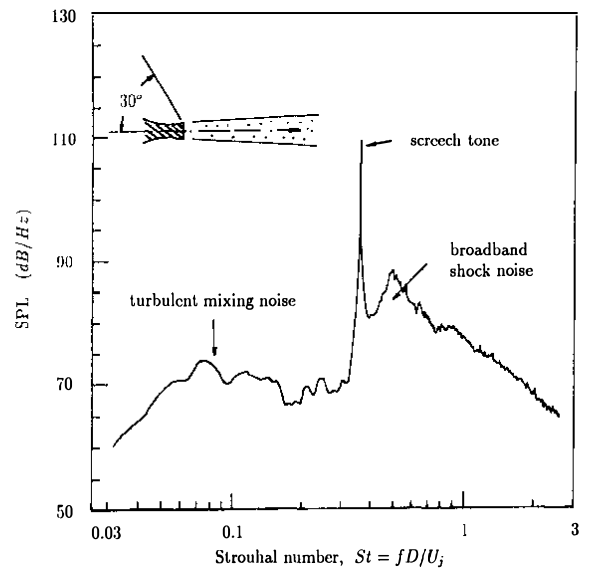
\includegraphics[width=3in]{images/noise.png}
	\caption{Supersonic jet noise spectrum, Seiner 1984, as published in Tam\cite{tam3}}
	\label{fig:noise}
\end{figure} 

\noindent
Turbulent mixing noise is predominantly due to large turbulent structures moving at supersonic speeds leading to phenomenon like mach wave radiation. Although fine turbulent structures also contribute to what is considered background noise, they are not as dominant as they are in subsonic flows. This noise is high at lower angles to jet and decreases as we move upstream.\\
\par\par

\noindent
Broadband shock noise (BBSN) is due to the interaction between turbulent structures and quasi periodic shock cells in the flow. Perfectly expanded flow is ideally not expected to encounter this noise since there should be no shocks/expansions to be 
reflected by mixing layer. Since the shocks cells are very well defined, the directivity and strength of this noise is much easier to formulate analytically unlike subsonic noise. This noise dominates at higher angles upstream\\ 
\par

\noindent
Screeching noise, easiest to notice in the fig \ref{fig:noise}, is considered to be a special case of broadband shock noise. When the turbulent structures interact with shock cell, acoustic waves are generated. These waves, of certain frequency band, travel outside jet and interact with lip region which inturn affects the generation of turbulent structures completing a feedback loop. It is important to note that the peaks of broadband shock noise and turbulent mixing noise vary with the observation angle (angle with respect to jet axis, 0 being along the jet). But the frequency of screech tone is same for all observation points. More interestingly, its frequency  always forms lower bound of broadband shock peak and they tend to merge as the angle increases. Infact, if we use angle $180^0$ in the formula to calculate the peak frequency of BBSN, we get the frequency value of screech tone \cite{tam1}.\\
\par 
As we have seen, frequency analysis of pressure data goes a long way to explain noise mechanisms. This report is to use similar techniques to study various scales of velocity and TKE data from steady PIV. Since we don't have time data, wavelength analysis has been done and compared with analytical shock cell information. 

%\end{document}
%\documentclass{report}
%\usepackage{fullpage}
%%\usepackage[top=1in, bottom=1in]{geometry}
%\usepackage{amsfonts}
%%for math symbols, Ex: \mathbb{N}
%\def\Definition{what does something mean}
%\usepackage{graphicx}
%\usepackage[hidelinks]{hyperref}
%\usepackage{pdfpages}
%\usepackage{float}
%\usepackage{subcaption}
%
%\begin{document}

\chapter{Methodology}

\section{Setup}

All the experimental data has been collected by Pablo et.al\cite{pablo}. Heated Jet Noise Rig, dual CCD cameras, dual pulse Nd:YAG Laser, 1.0$\mu$ Aluminium Oxide as particle seeds, Olive oil as ambient seed,  C-D conical nozzle of diameter($D_e$) 0.813in and design mach number 1.5, 12 equally distributed chevrons with length 0.2D and spacing 0.08D have been used for the setup. Each of the four images taken are of resolution 130*170(w*h) with spacing of about 2mm (0.01$D_e$) and then merged to form complete domain. \\

\begin{figure}[H]
\begin{subfigure}{.5\textwidth}
	\centering
	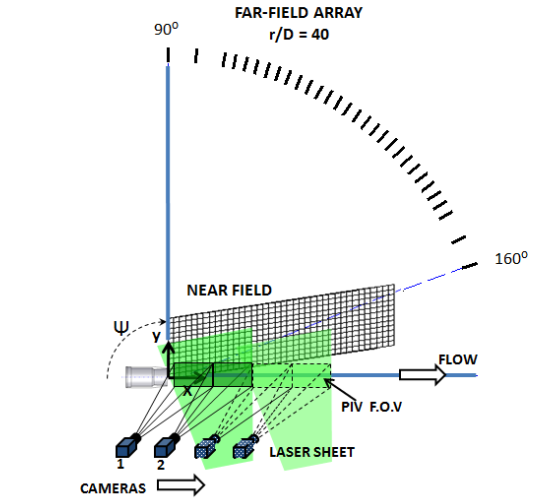
\includegraphics[width=3in]{images/setup.png}
	\caption{Experimental setup}
	\label{fig:setup1}
\end{subfigure}%
\begin{subfigure}{.5\textwidth}
	\centering
	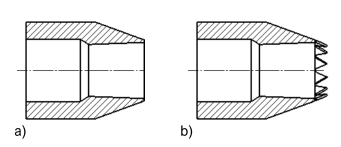
\includegraphics[width=3in]{images/nozzles.png}
	\caption{Nozzles with and without chevrons}
	\label{fig:setup2}
\end{subfigure}
\caption{Nozzles and Experimental setup by Pablo Mora et.al.,}
\label{fig:setup}
\end{figure}

\par\par
Python3.6 has been used to convert experimental column data into array form and create all the plots. Complete code\footnote{ Code and \LaTeX \ files can also be accessed on https://github.com/ravirejo/PIVAnalysis.} is included in the appendix. The only steps to be taken to run the code is to ensure that exit diameter(dia), temperature ratio (NTR) and pressure (NPR) are updated manually in the code (\textit{TRPR }array) and the centre of jet has to be adjusted according to the experimental data. Input files expected are B0001up, B0001Down for \textit{$V_x$}; B0002up, B0002Down for \textit{$V_y$}; B0004up, B0004Down for \textit{TKE} with \_ntr\_npr added to their names where ntr, npr are numerical values in the form of 1p0, 3p6 etc.,

\begin{figure}[H]
\begin{subfigure}{.5\textwidth}
	\centering
	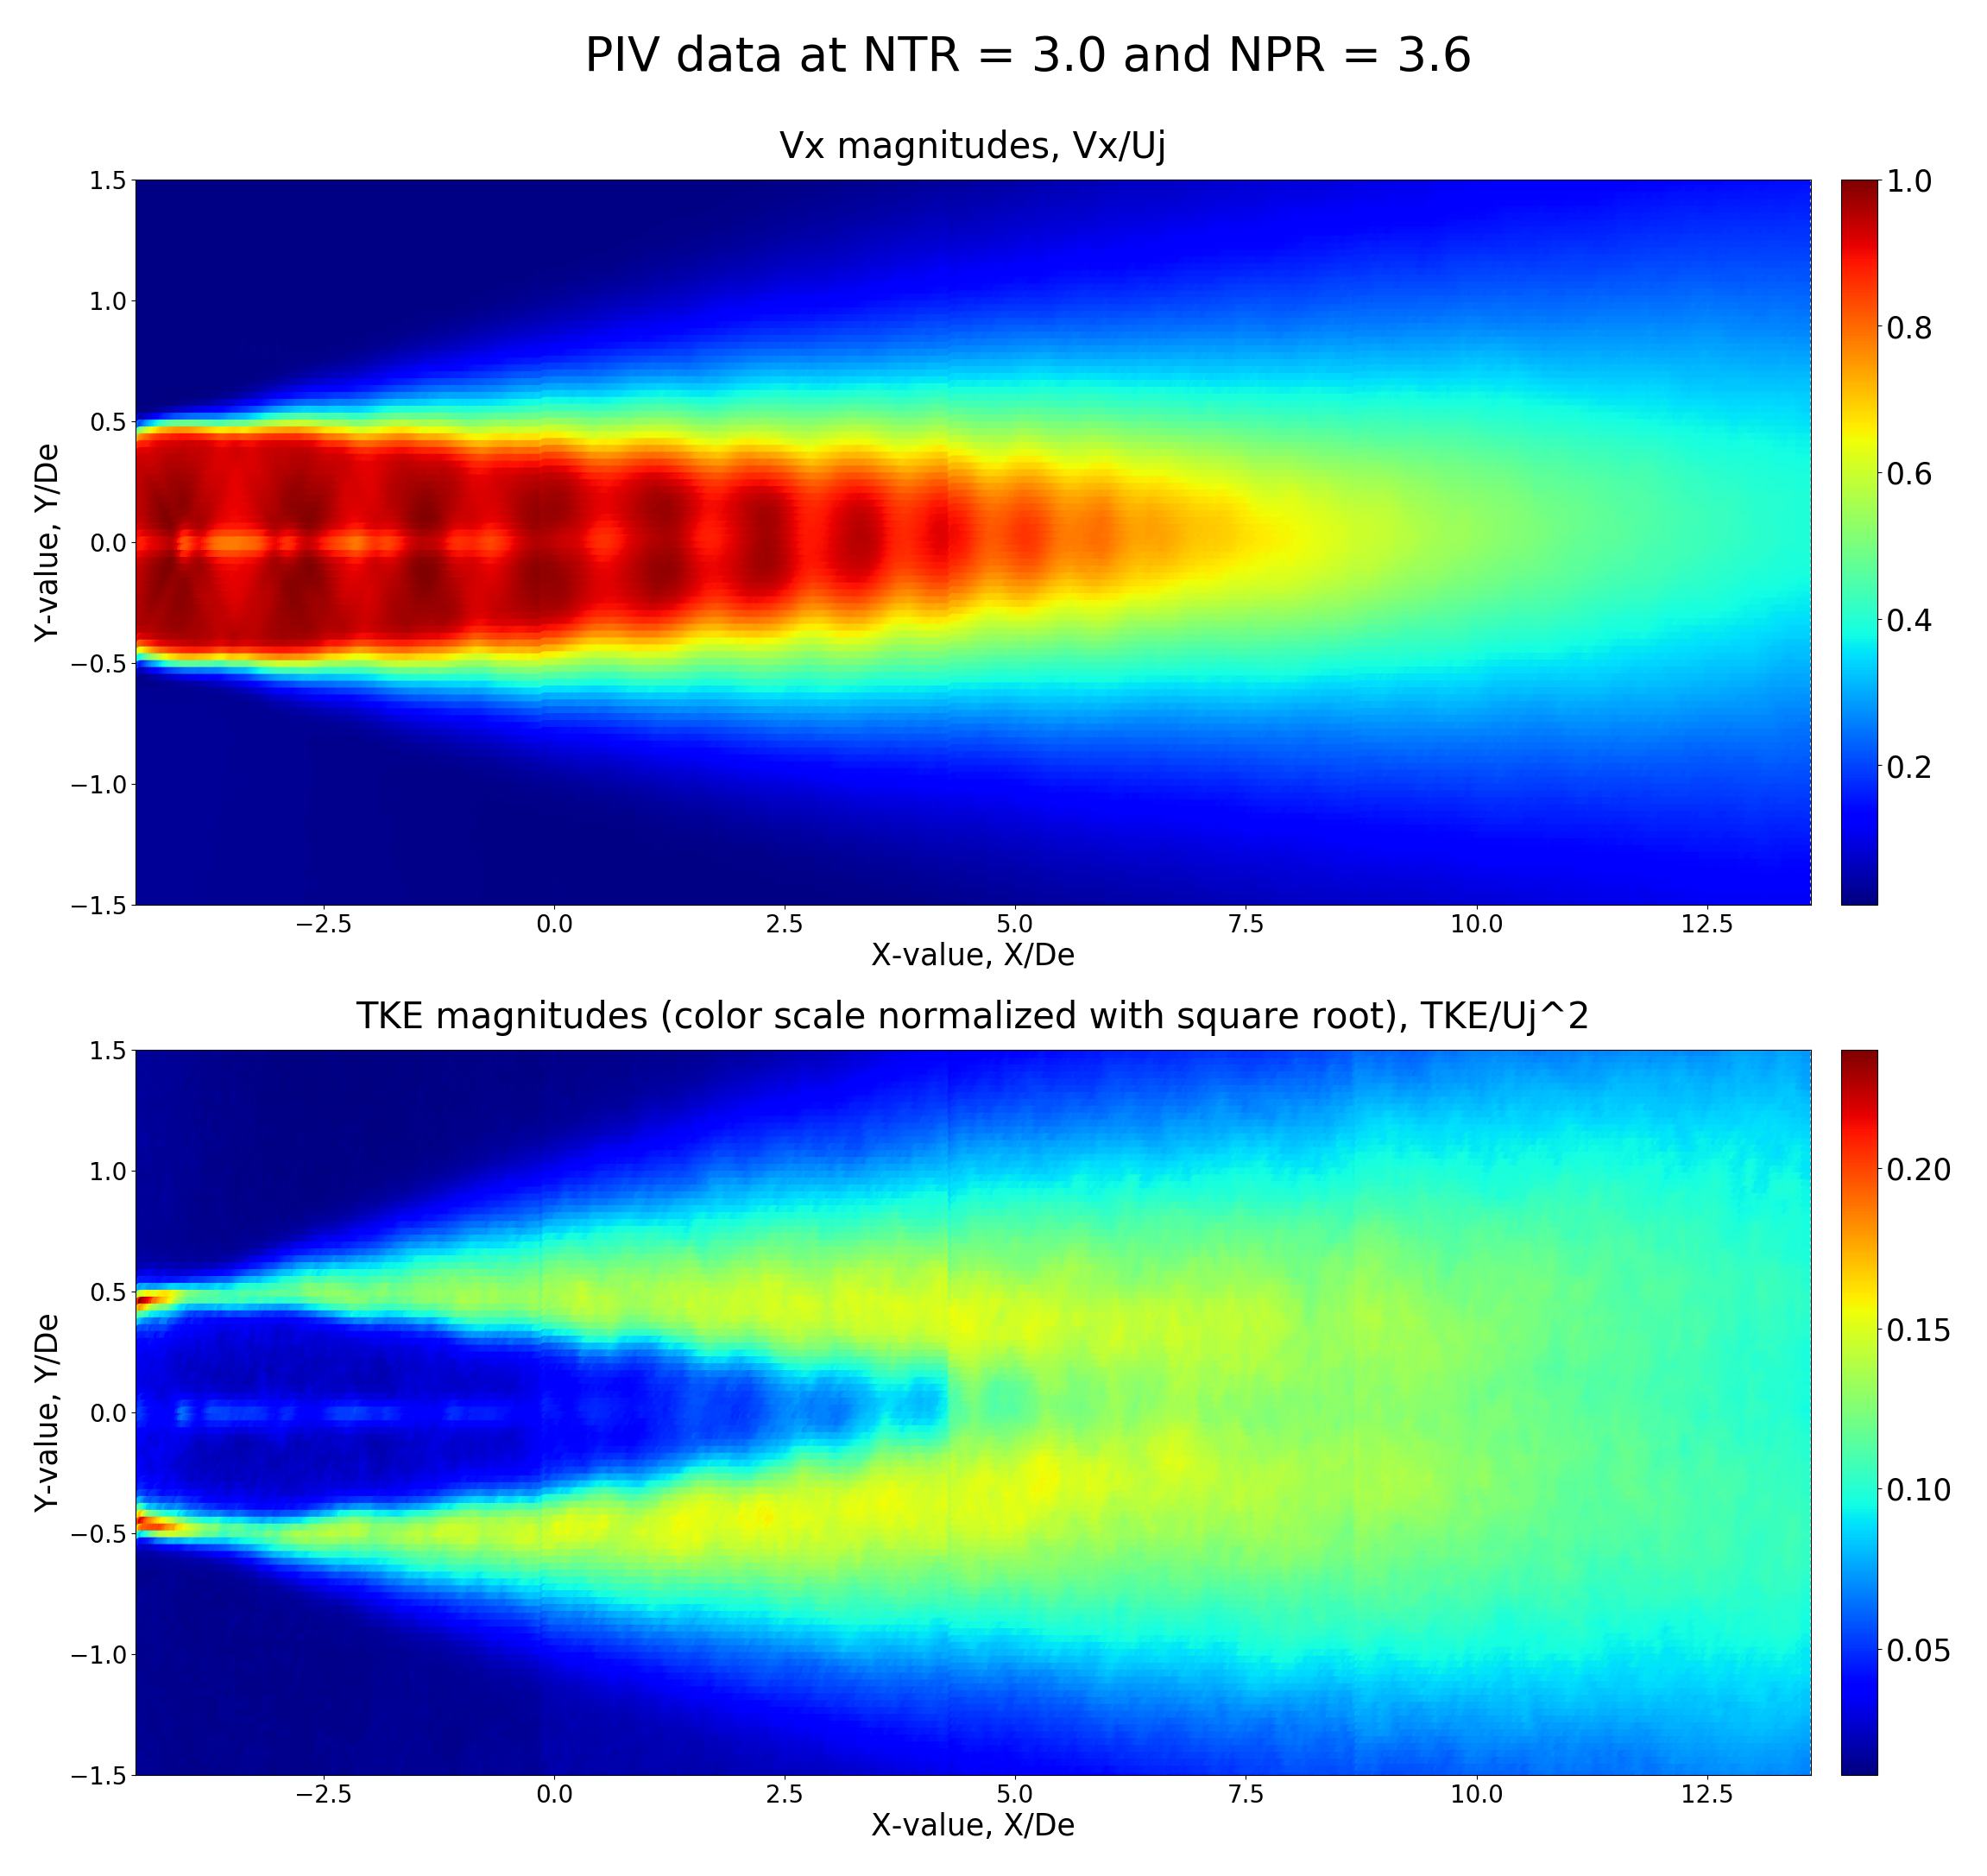
\includegraphics[width=3in]{images/2dsample.png}
	\caption{TKE and Vx at NTR 3.0, NPR 3.6}
	\label{fig:2dsample}
\end{subfigure}%
\begin{subfigure}{.5\textwidth}
	\centering
	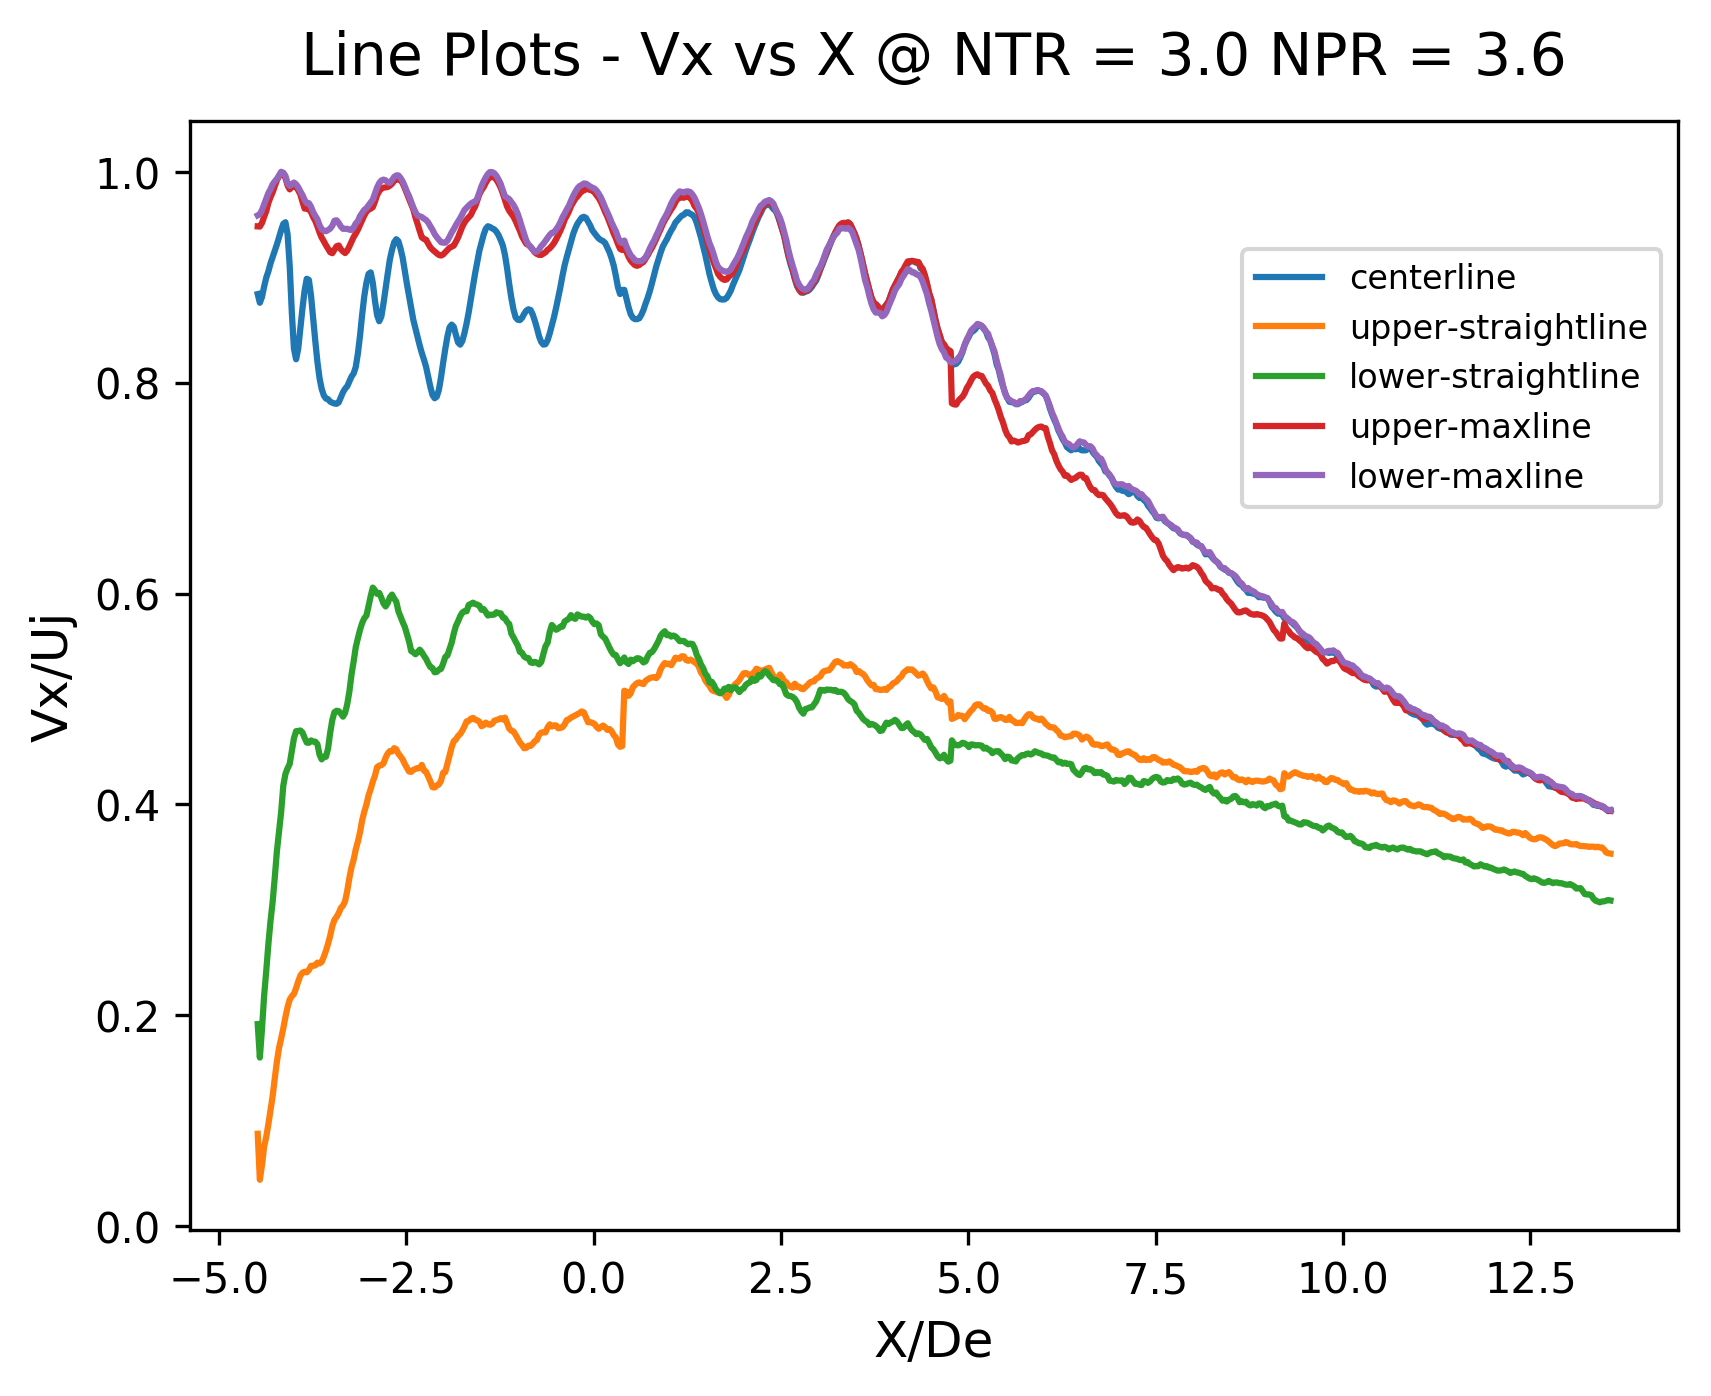
\includegraphics[width=3in]{images/lineplotsample.png}
	\caption{Lineplot of Vx at NTR 3.0, npr 3.6}
	\label{fig:lineplotsample}
\end{subfigure}
\caption{ Domain plot for TKE and Vx, Lineplot for Vx at NTR3.0, NPR3.6.}
\label{fig:2d&lineplot}
\end{figure}

\section{2D image reconstruction}
Both Velocity and Turbulent Kinetic Energy (TKE) (fig \ref{fig:2dsample}) have been normalized with $U_j$ and $U_j^2$ where $U_j$ is jet velocity i.e., max velocity at the exit of nozzle. 

\section{Lineplots}
Lineplots (fig \ref{fig:lineplotsample}) have been drawn for Vx, Vy and TKE for five lines; Centreline is along the centre of jet. Upper and lower straight lines are along the straight lines at lips of jet. Upper and lower maxlines are curves of maximum values above and below centreline. Due to the complexity of experimental setup, exact position of jet centre is not usually at origin and hence has to be accounted manually in the code. But slight discrepancy in vertical position should not be an issue in the present context, since we are more interested in length scales along X.

\begin{figure}[H]
\begin{subfigure}{.5\textwidth}
	\centering
	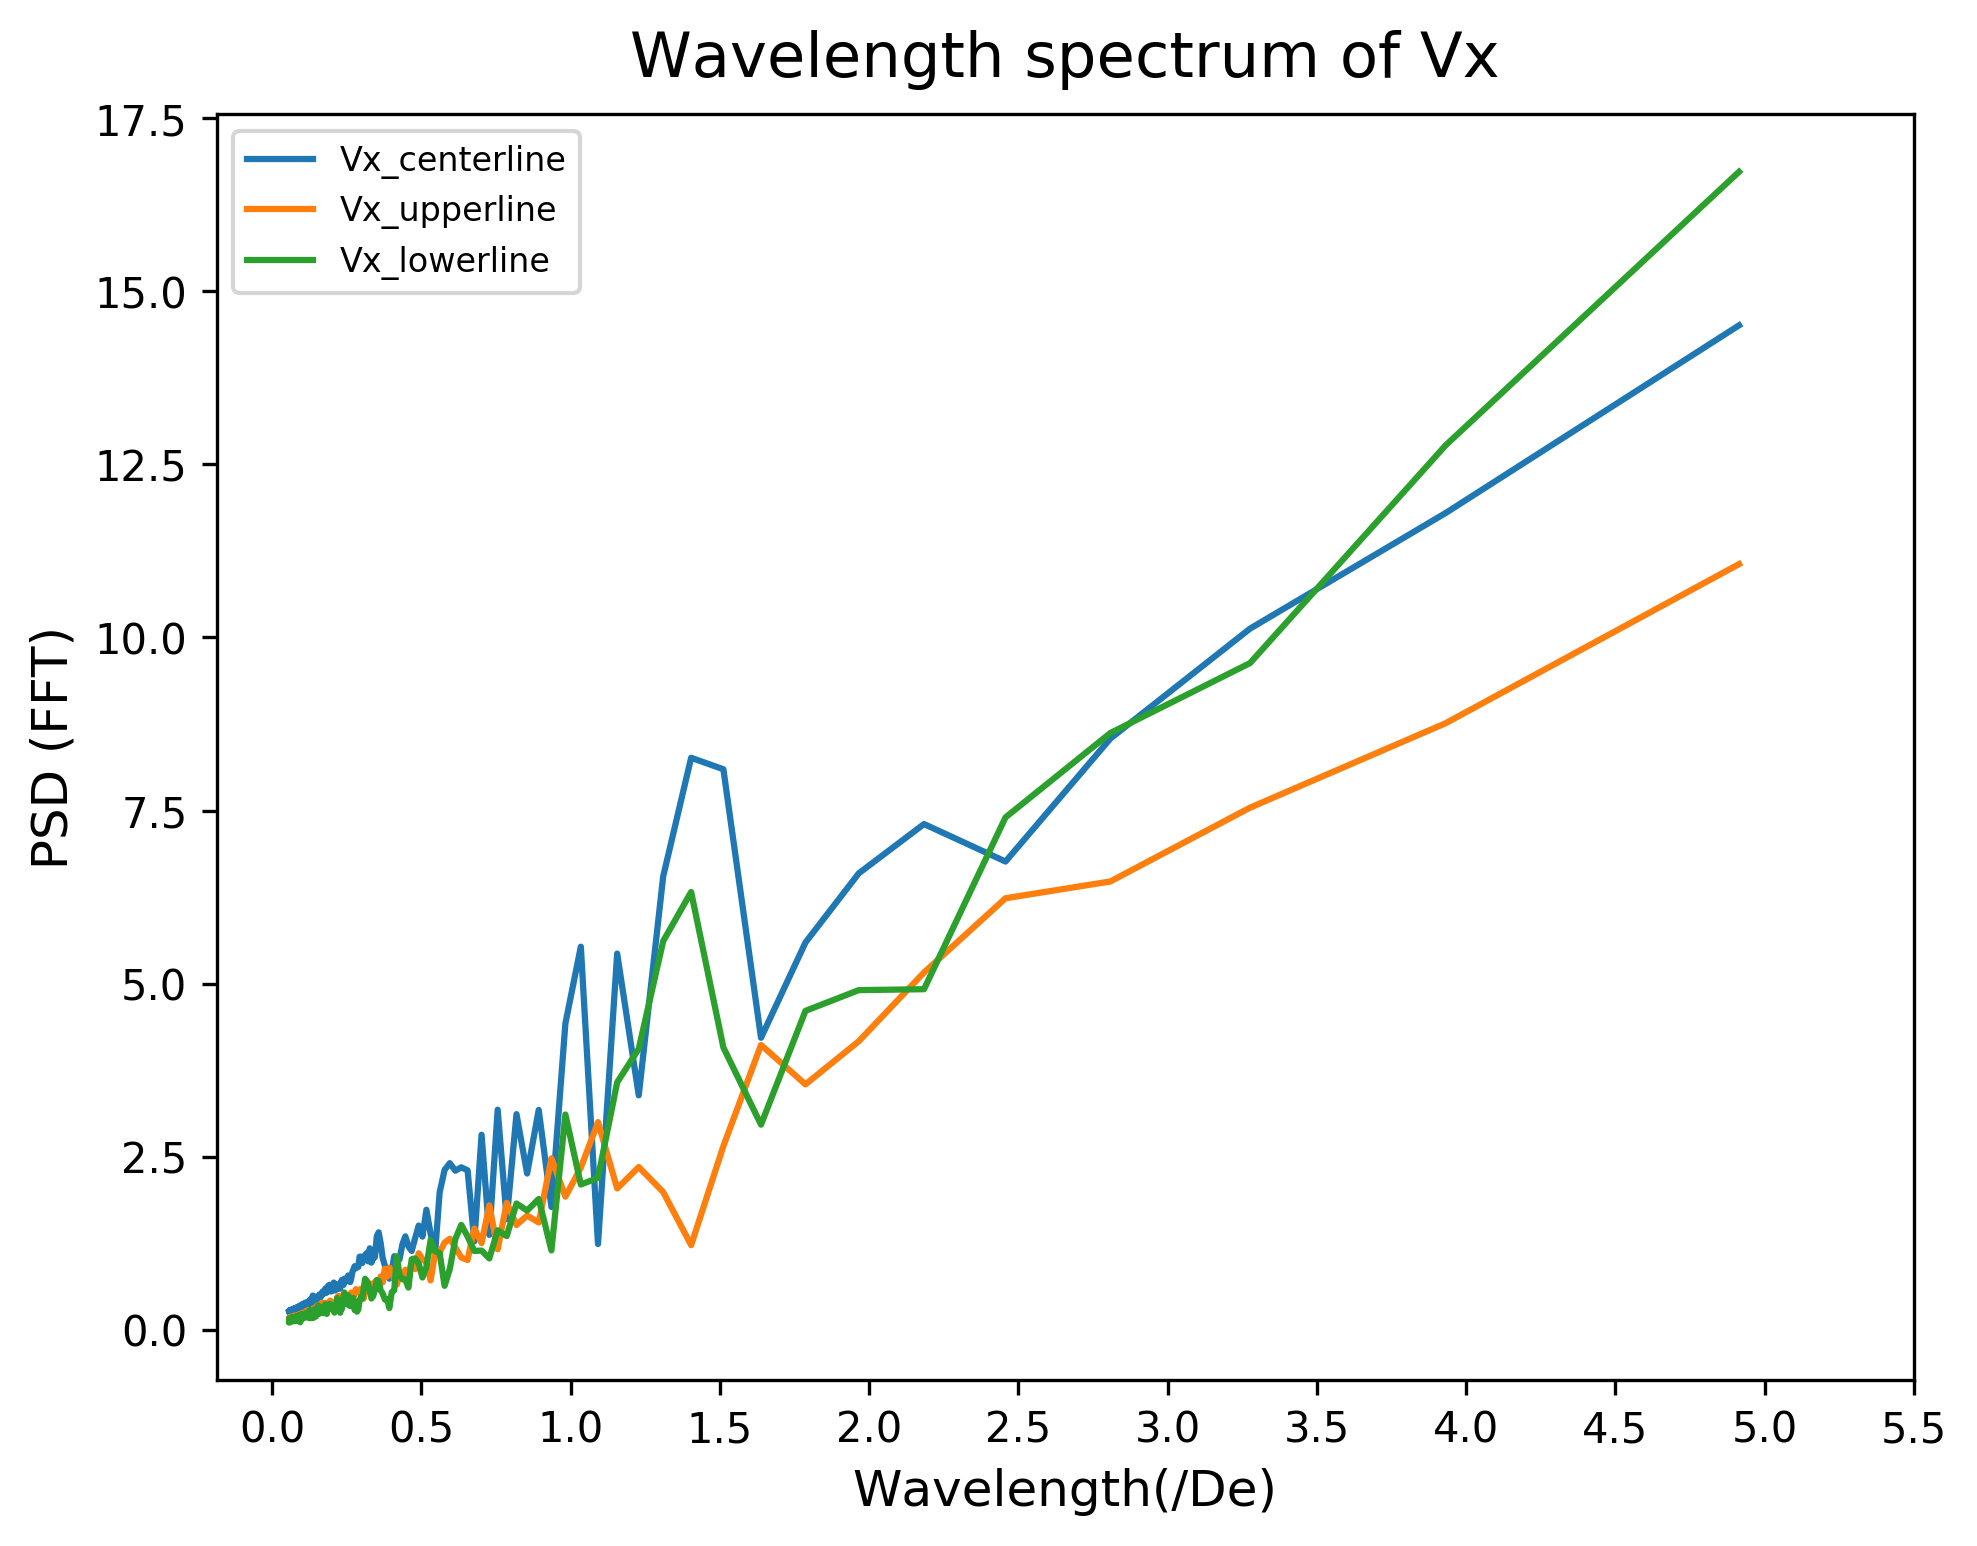
\includegraphics[width=1.5in]{images/fftsample.png}
	\caption{wavelength analysis for Vx at NTR 3.0, NPR 3.6}
	\label{fig:fftsample}
\end{subfigure}%
\begin{subfigure}{.5\textwidth}
	\centering
	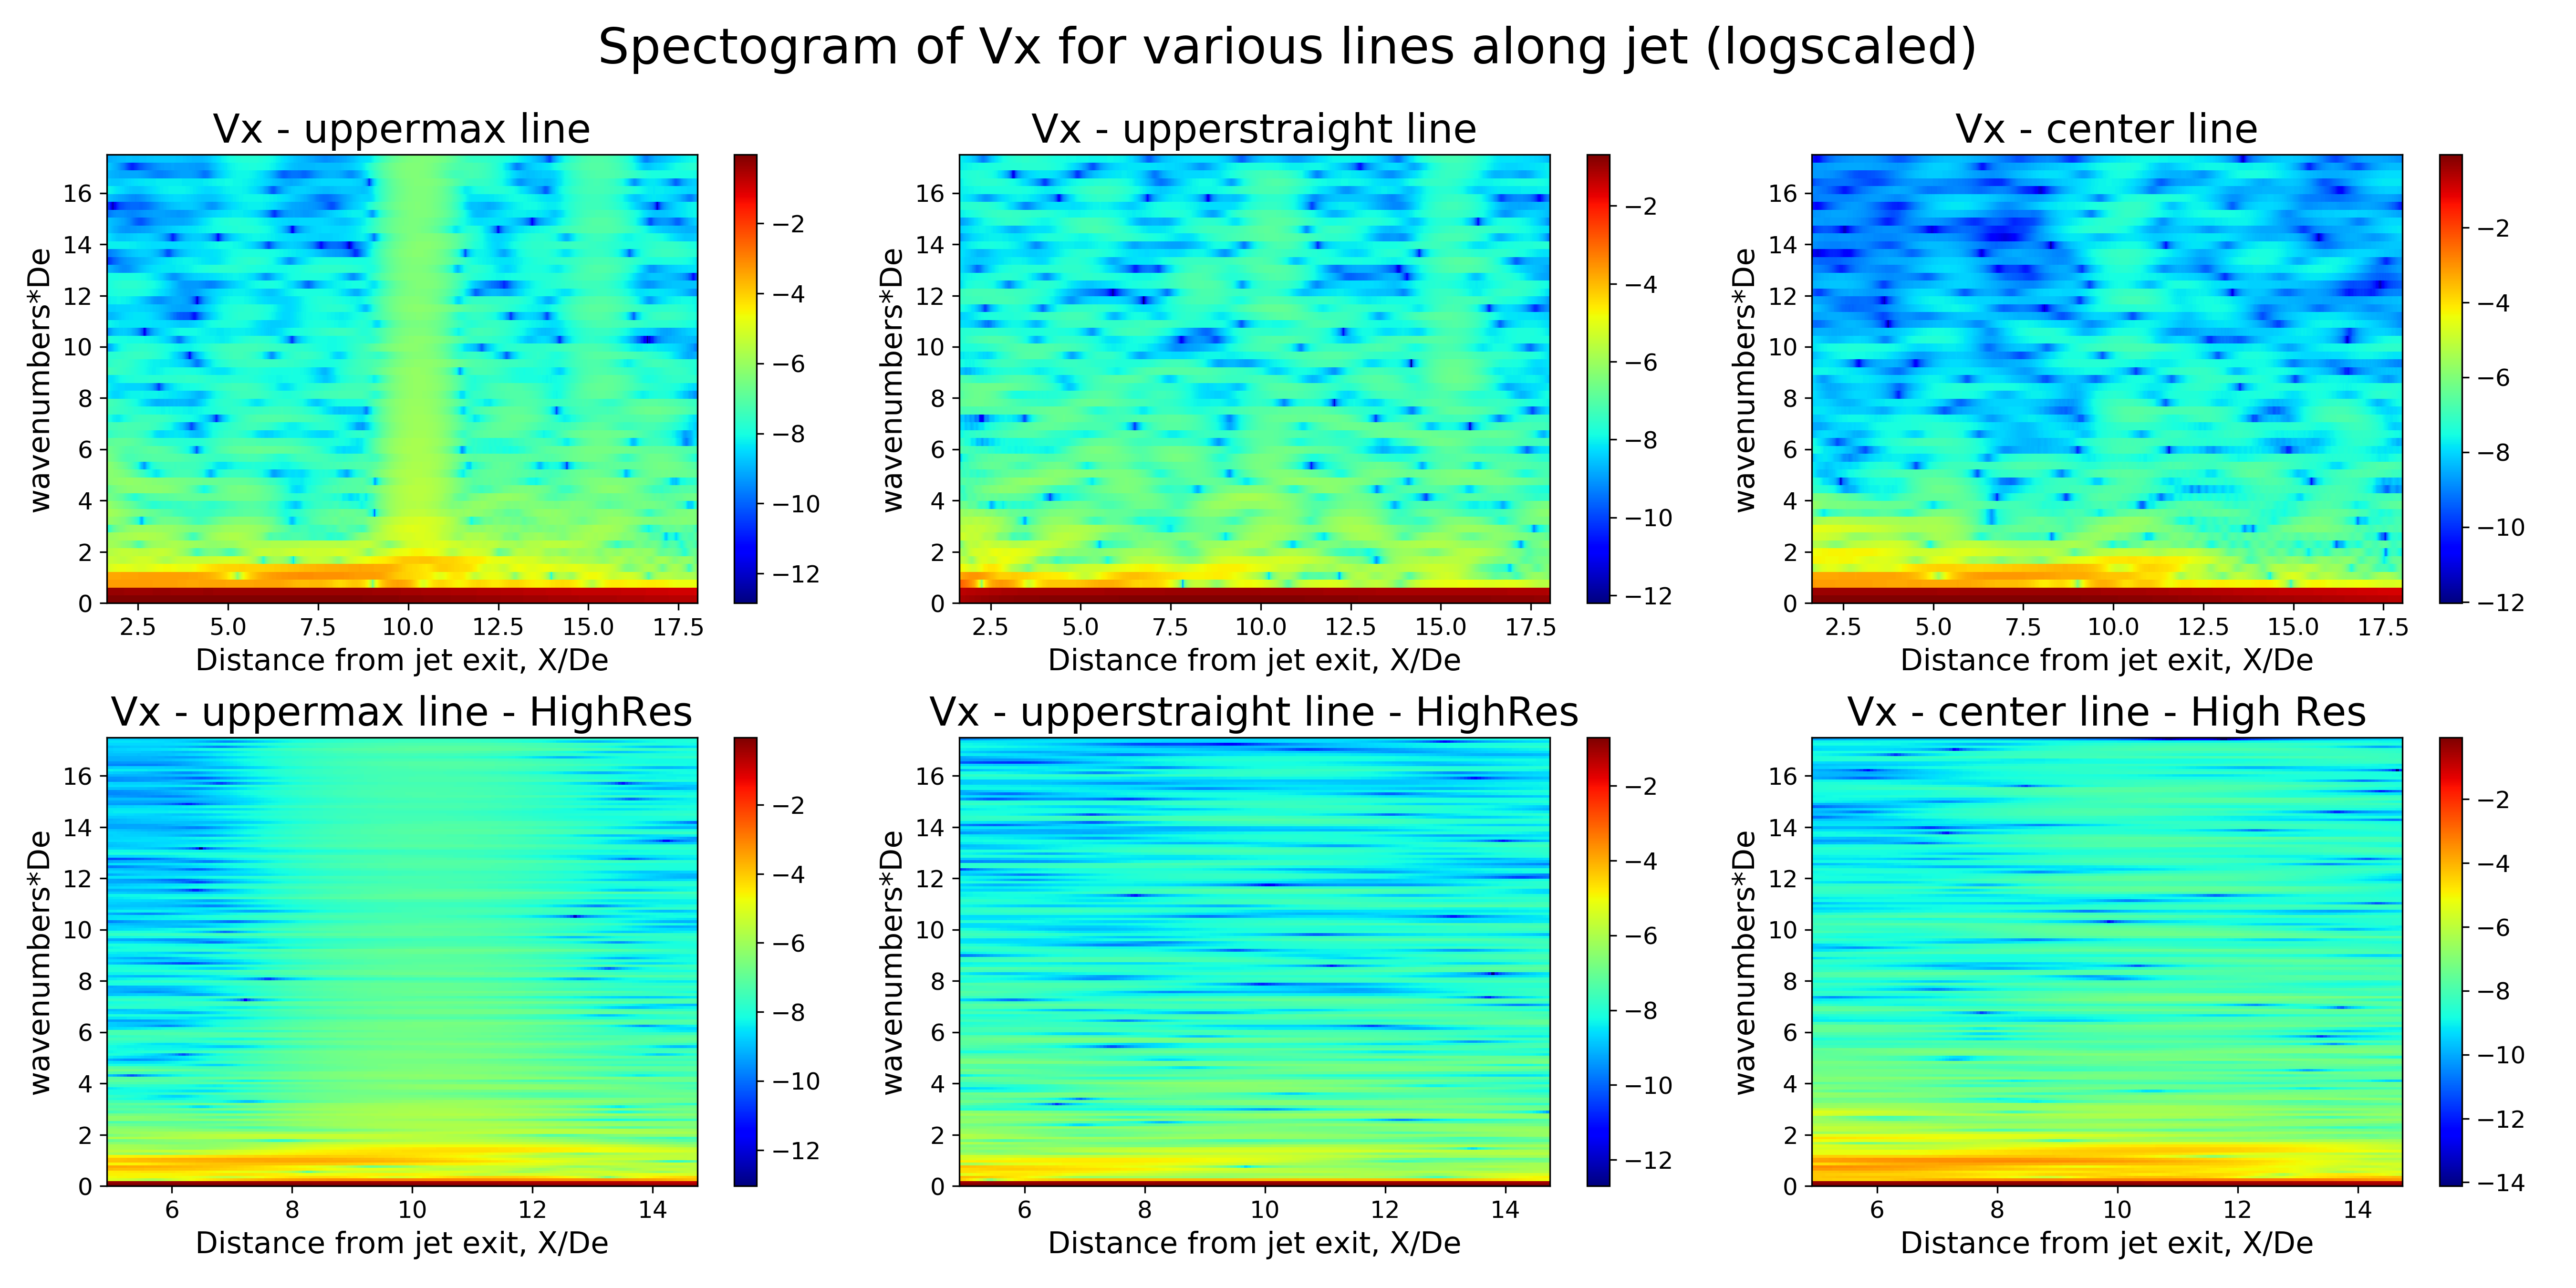
\includegraphics[width=2.5in]{images/spectogramsample.png}
	\caption{Spectogram of TKE at NTR 3.0, npr 3.6}
	\label{fig:spectogramsample}
\end{subfigure}
\caption{ Spectogram for TKE at NTR3.0, NPR3.6.}
\label{fig:fft&spectogram}
\end{figure}

\section{Spatial FFT}
Fast Fourier Transform (FFT) (fig \ref{fig:fftsample}) is a widely used technique to analyse various frequency components in an audio signal. Since we are restricted to steady state analysis for this report, we do not have time data. But we can still apply FFT to the line plot data and obtain velocity scale spectrum ( Power Spectral Density Vs Wavelengths). This can be used to study shock cell lengths and positions with a perspective different from previous methods. FFT has been calculated for three lineplots; centre, upper and lower straightlines. Resolution in x direction is about $1/40^{th}$ of $D_e$. After giving some margin, sampling interval is chosen as $1/35$. Linear increase in psd with wavelength could be detrended as we are only interested in the characteristic wavelengths, but has been ignored.

\section{Spectogram}
FFT is a great tool for component analysis but it does not give information at a specific time instant, or specific position in this context. Spectogram (fig \ref{fig:spectogramsample}) can be used for this purpose. Essentially, spectogram is short FFT taken over a chosen window of fragments of input signal and averaged if fragments are overlapping. So, we have spectrum at centre point of every fragment. Shorter the fragment, higher the resolution in x direction but we have to ensure the fragment is sufficiently longer than length of shock cell to ensure that the relevant wavelength is captured. Higher the overlap between fragments, smoother the transition. Resolution seems to increase in y (wavenumber) direction as observed in \ref{fig:spectogramsample}. But the output to input domain ratio is far less than 1 since the spectogram starts only from the centre of first fragment. Moreover, precision decreases in the direction of x as the signal is smeared because of high overlap. 

\section{Shockcell Length}
Shockcell length has been calculated from the analytical equation derived by Tam et.al \cite{tam1}.

\begin{equation}\label{eq:1}
L_s \approx \ \pi \sqrt{(M_j^2-1)} D_j/\mu, \ where \ \mu \ = \ 2.40483
\end{equation}

$D_j$, diameter of jet along the flow, is higher or lower than $D_e$ depending on whether the flow is underexpanded or overexpanded. $M_j$, mach number at the jet centre, generally decreases along the jet as expected. 

%\end{document}
%\documentclass{report}
%\usepackage{fullpage}
%%\usepackage[top=1in, bottom=1in]{geometry}
%\usepackage{amsfonts}
%%for math symbols, Ex: \mathbb{N}
%\def\Definition{what does something mean}
%\usepackage{graphicx}
%\usepackage[hidelinks]{hyperref}
%\usepackage{pdfpages}
%\usepackage{float}
%\usepackage{subcaption}
%
%\begin{document}

\chapter{Analysis}

2D plots for velocity and TKE (fig \ref{fig:2dplots}) are a great way to get a qualitative view of the whole domain. But often they require careful scaling and tend to have overwhelming information in some cases. We can look to other methods to get more specific observations.

\begin{figure}[H]
\begin{subfigure}{.5\textwidth}
	\centering
	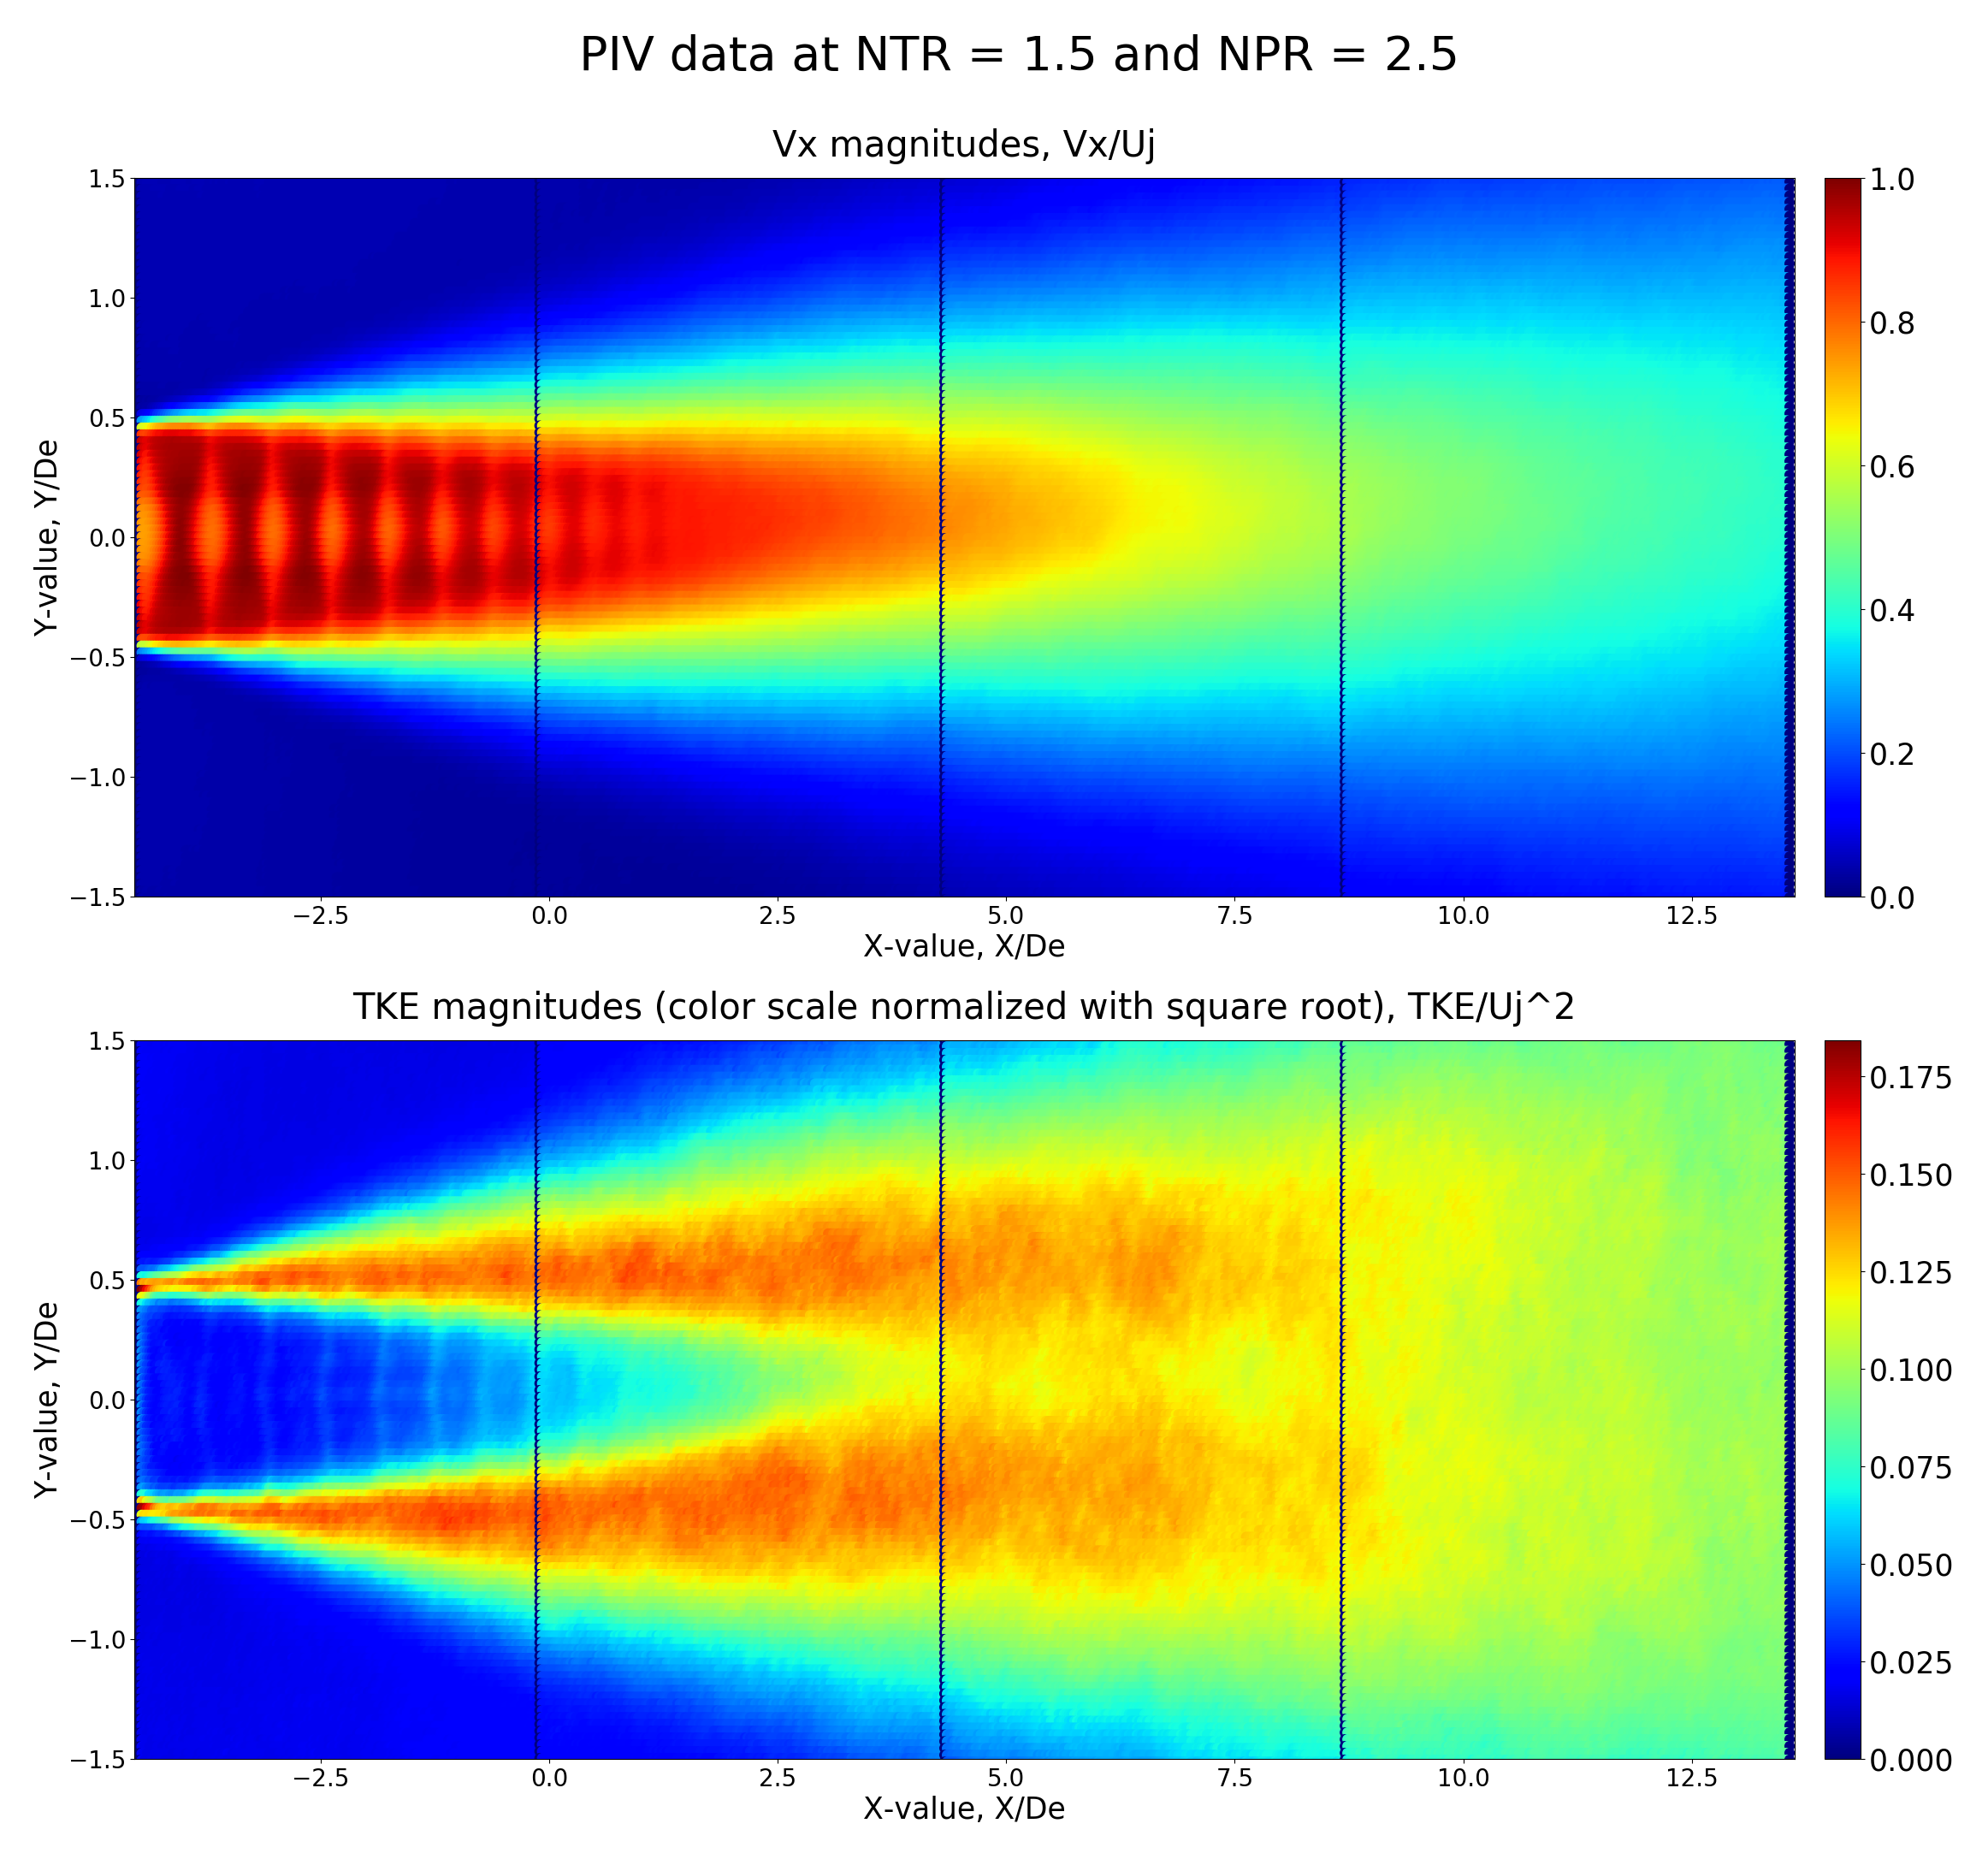
\includegraphics[width=2.3in]{images/PIV_NTR1p5_NPR2p5.png}
	\caption{NTR:1p5 NPR:2p5 }
	\label{fig:2dplots1p52p5}
\end{subfigure}%
\begin{subfigure}{.5\textwidth}
	\centering
	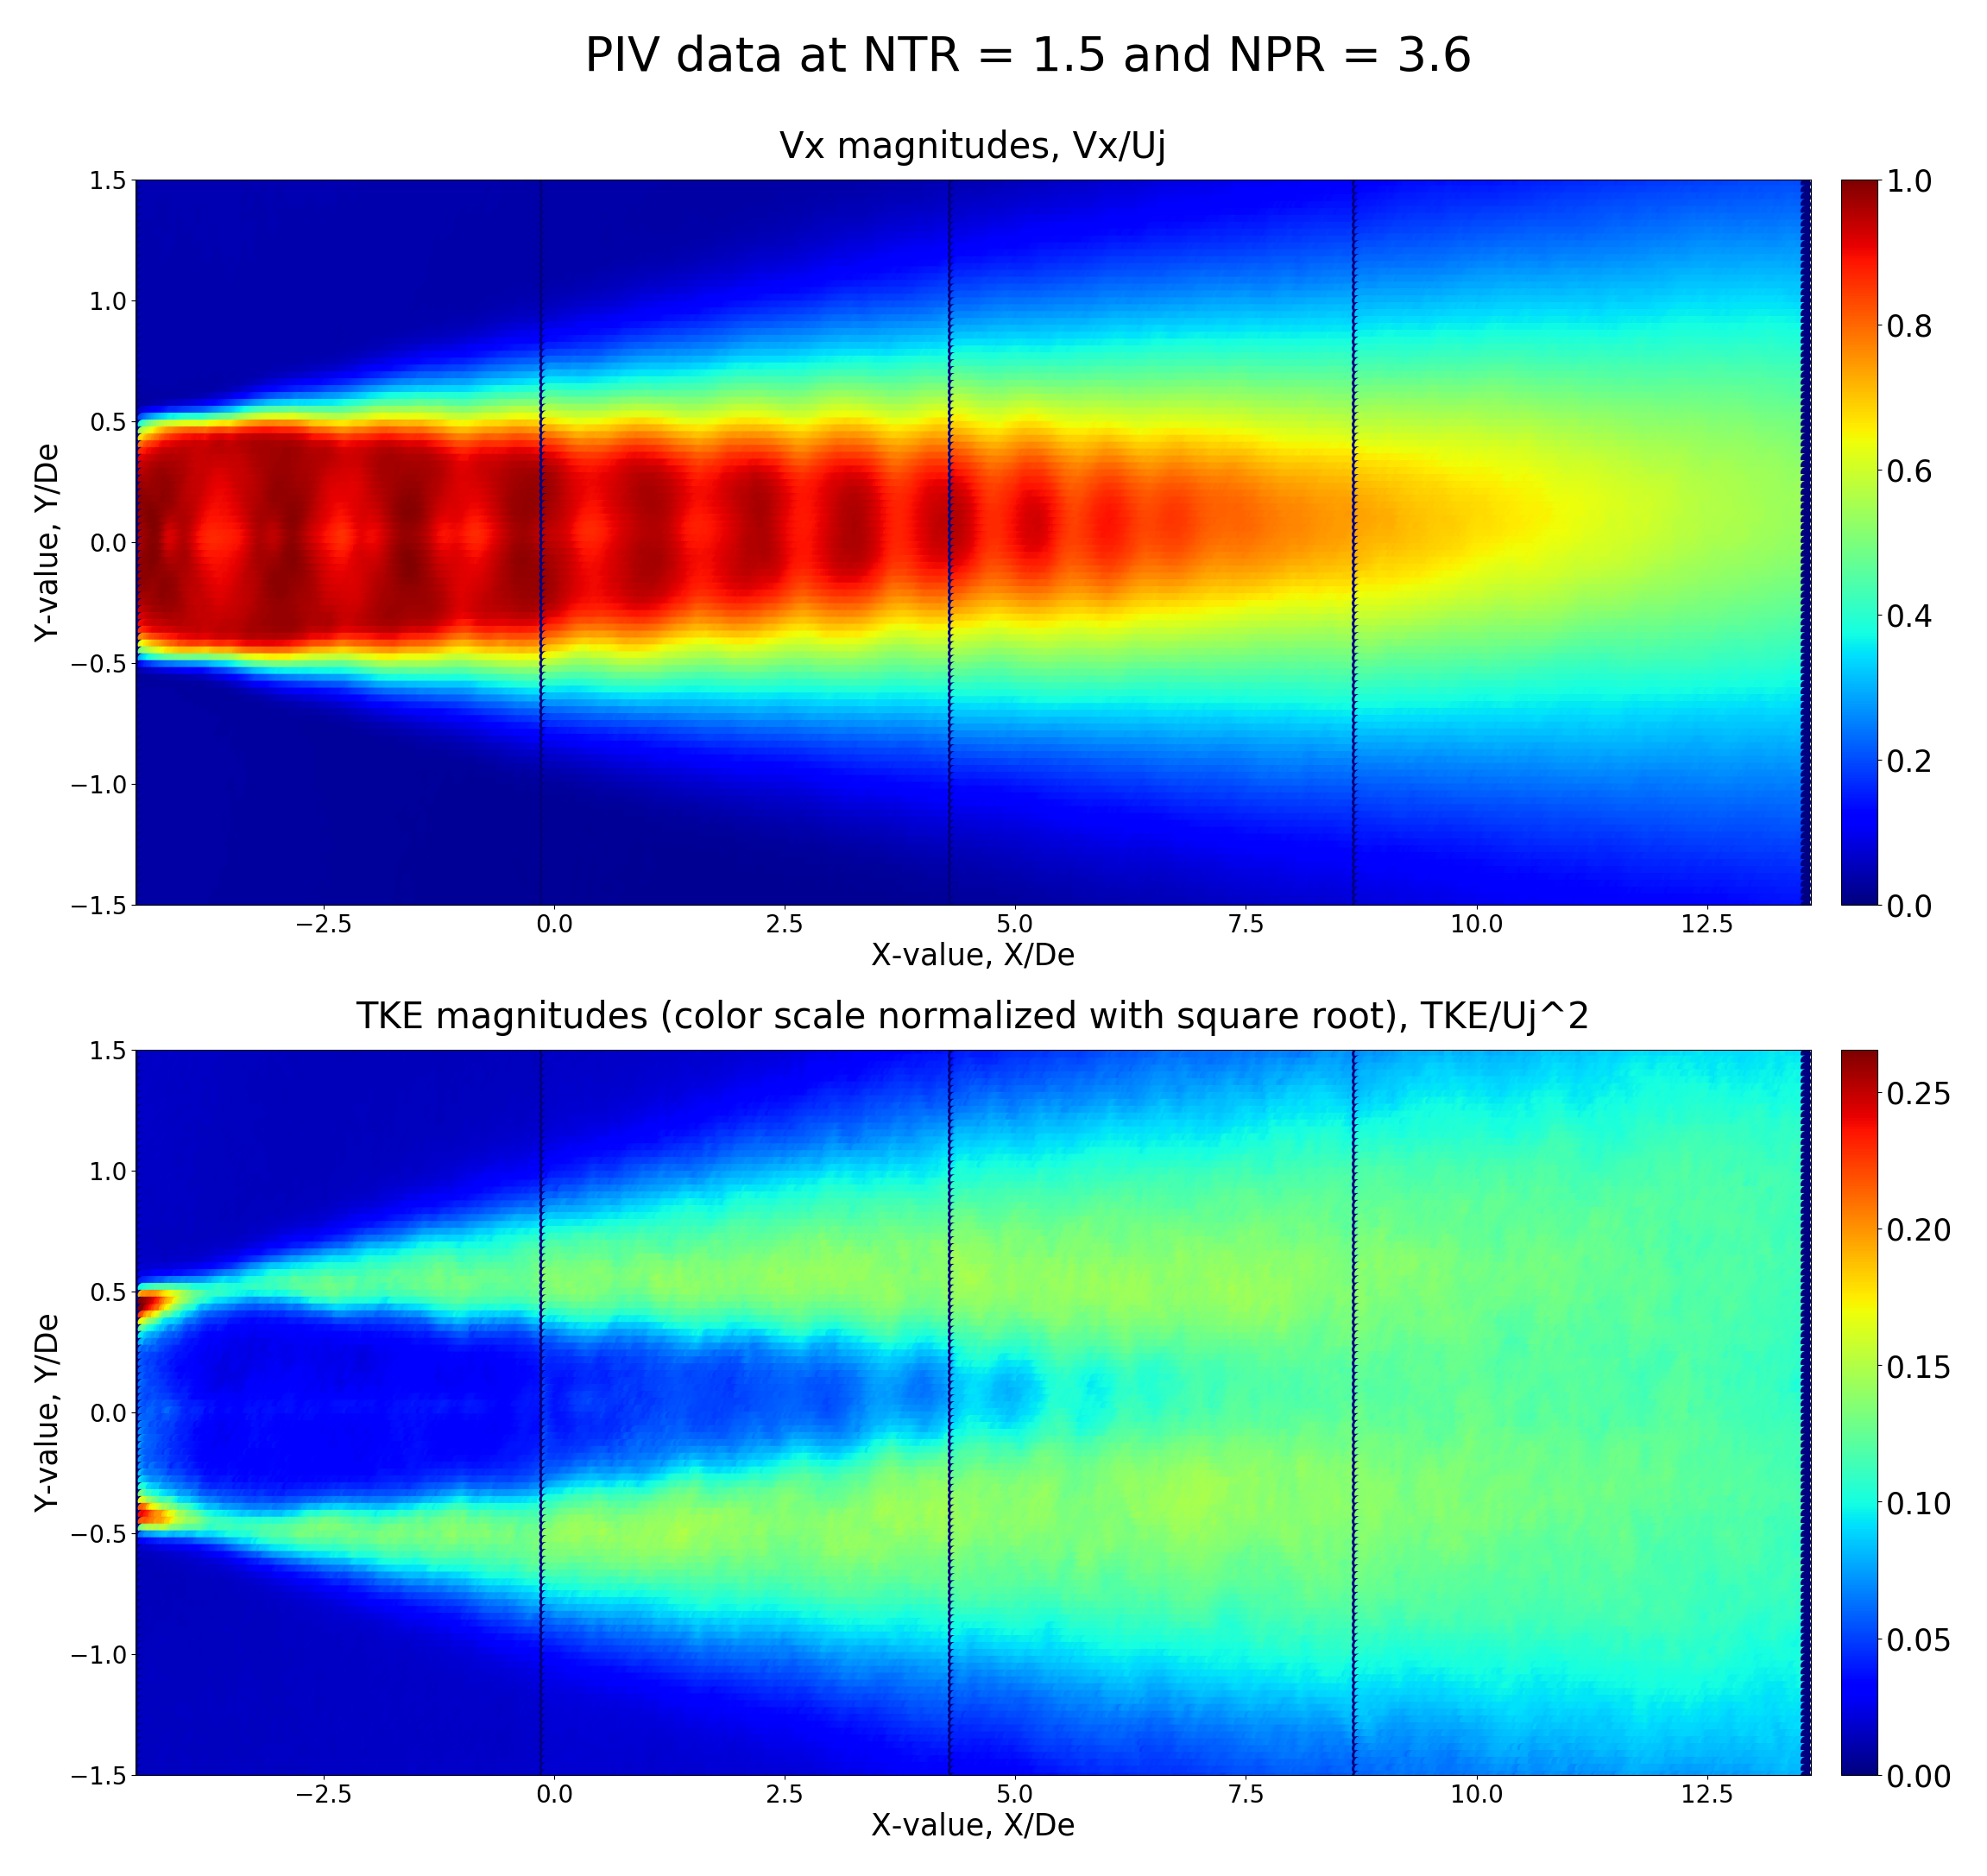
\includegraphics[width=2.3in]{images/PIV_NTR1p5_NPR3p6.png}
	\caption{NTR:1p5 NPR:3p6 }
	\label{fig:2dplots1p53p6}
\end{subfigure}
\begin{subfigure}{1.0\textwidth}
	\centering
	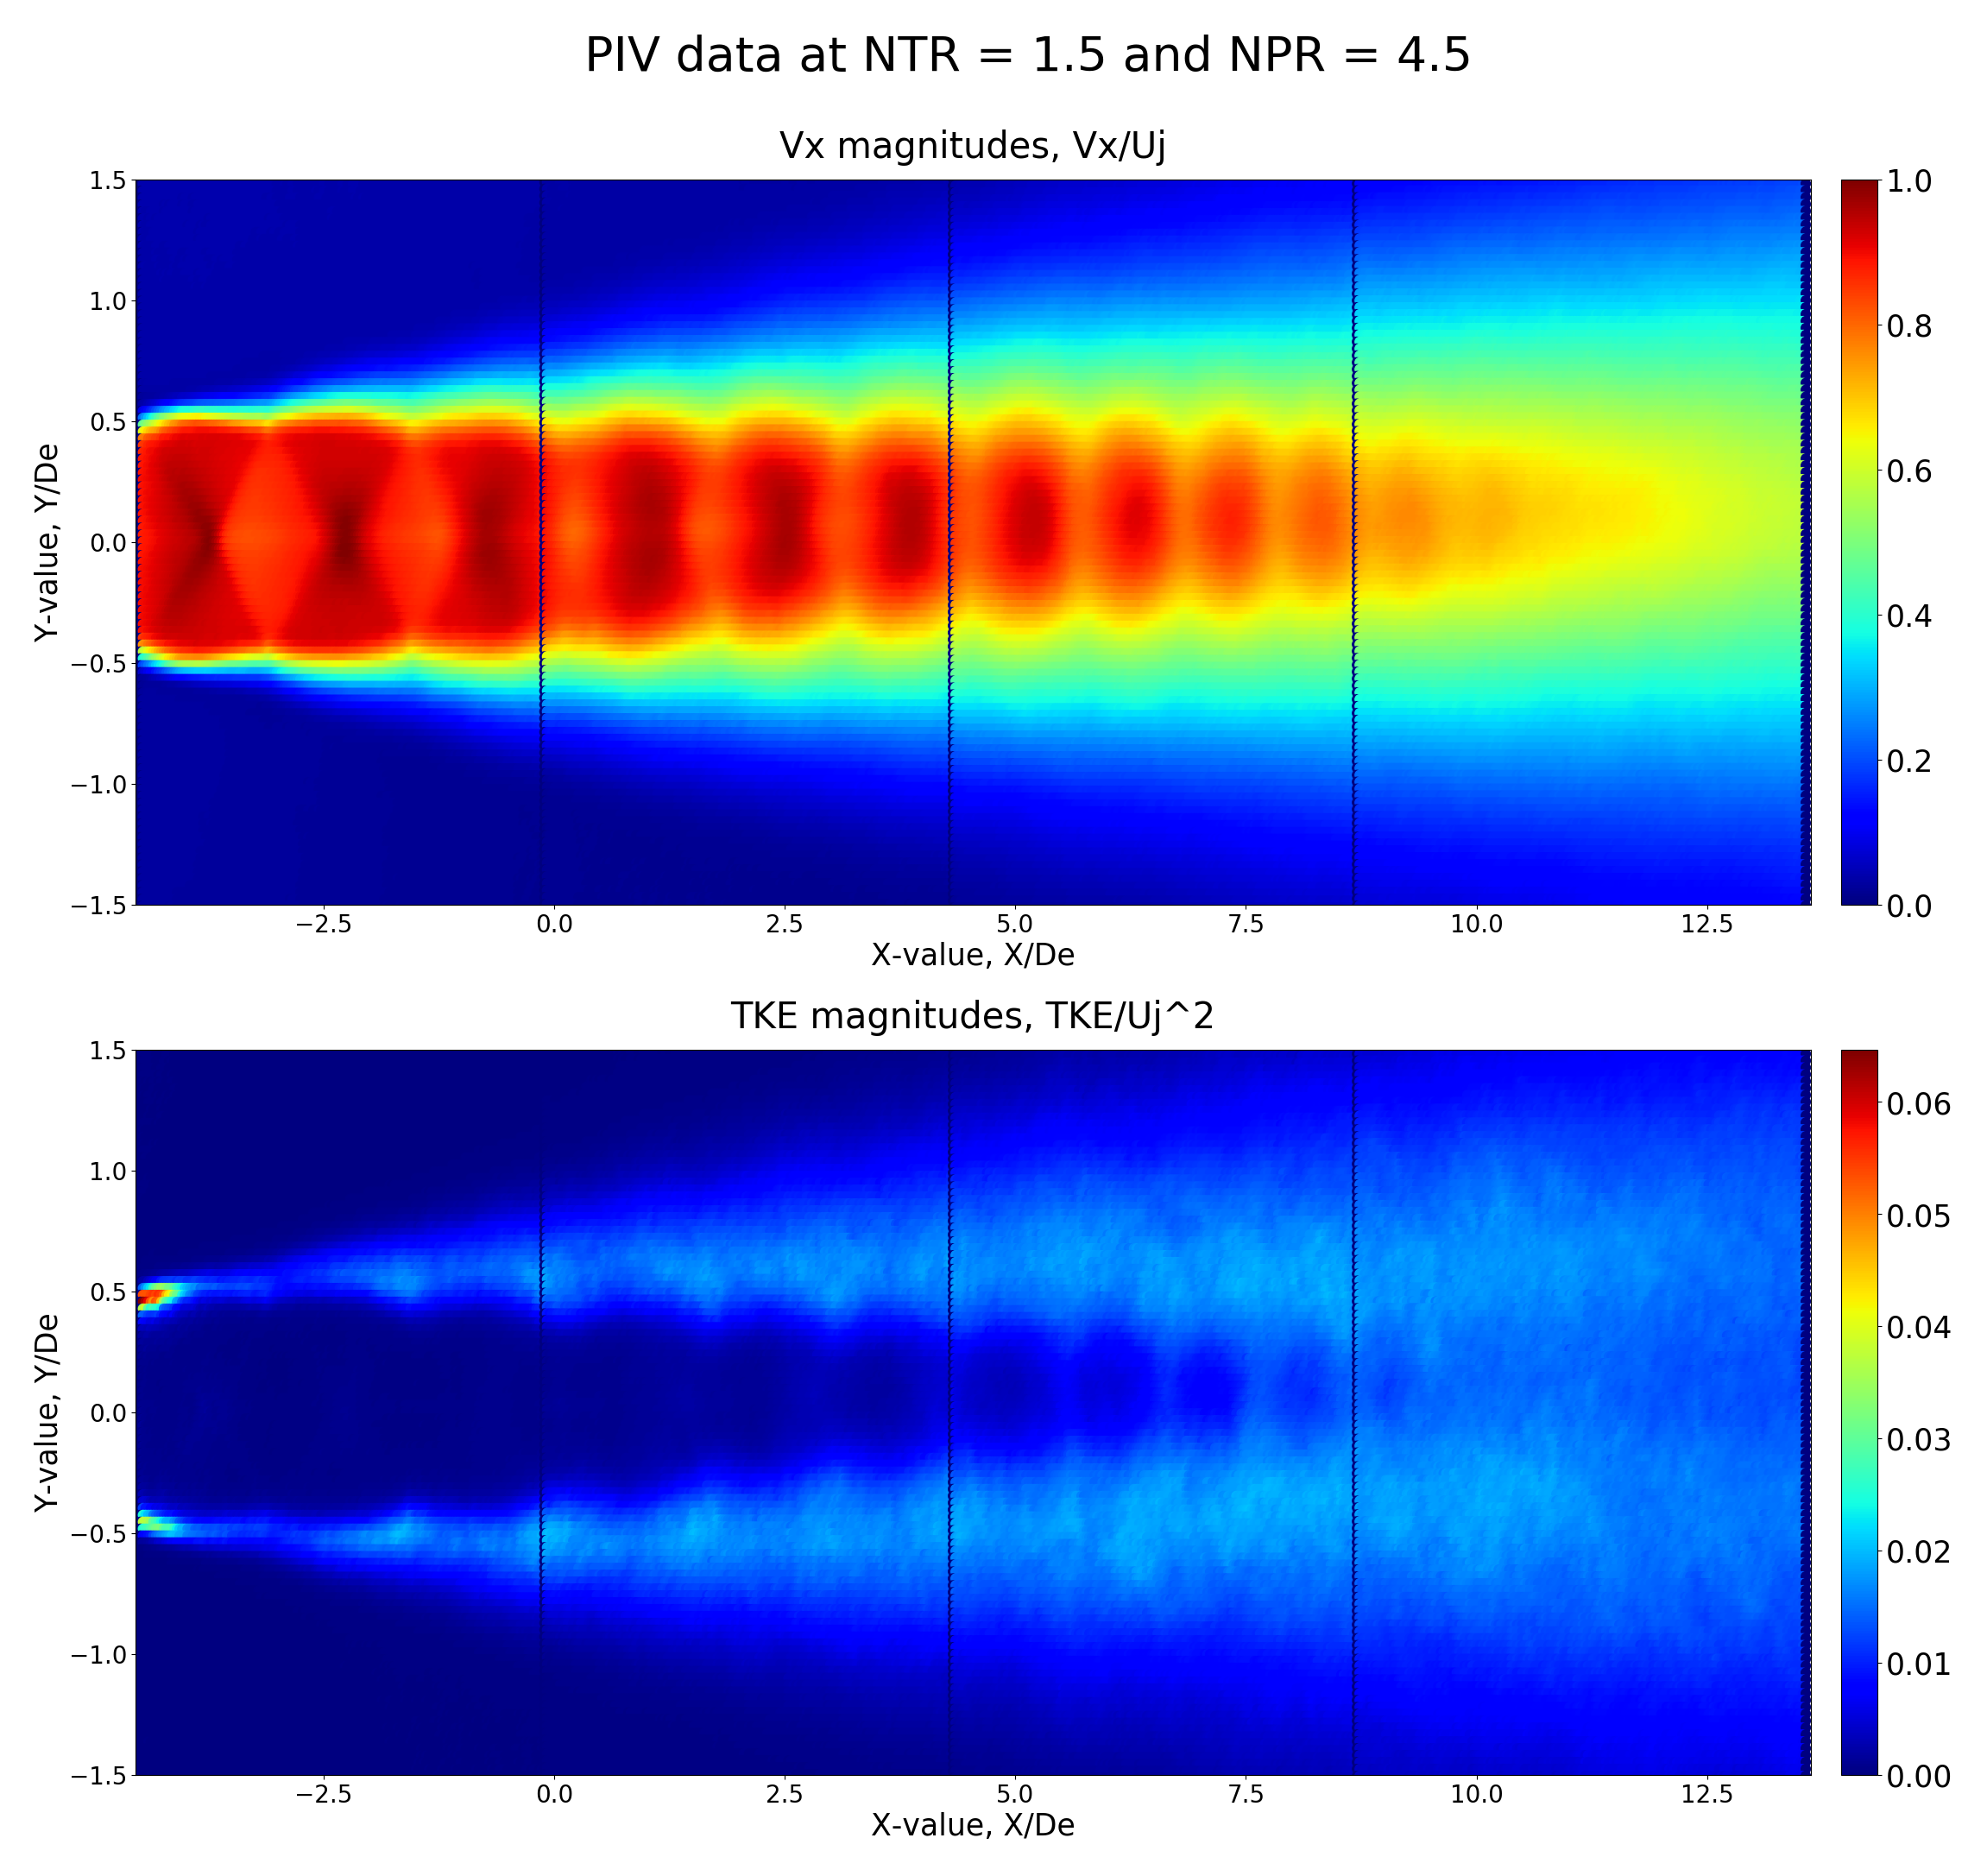
\includegraphics[width=2.3in]{images/PIV_NTR1p5_NPR4p5.png}
	\caption{NTR:1p5 NPR:4p5 }
	\label{fig:2dplots1p544p5}
\end{subfigure}
\caption{$V_x$, TKE without chevrons at $M_d$ 1.5 }
\label{fig:2dplots}
\end{figure}

\section{Shock cell length}
For an ideally expanded flow; assuming $D_j$, $M_j$ same as $D_e$,$M_d$; shock cell length can be calculated from equation \ref{eq:1}  to be 1.46$D_e$. It is expected to be higher for underexpanded flow and lower for overexpanded flow because of the differences in $D_j$ and $D_e$. Since $M_j$ decreases along the flow, this shock length is usually among the highest of all the wavelengths seen in the spectrum.\\ 

\begin{figure}[H]
\begin{subfigure}{.5\textwidth}
	\centering
	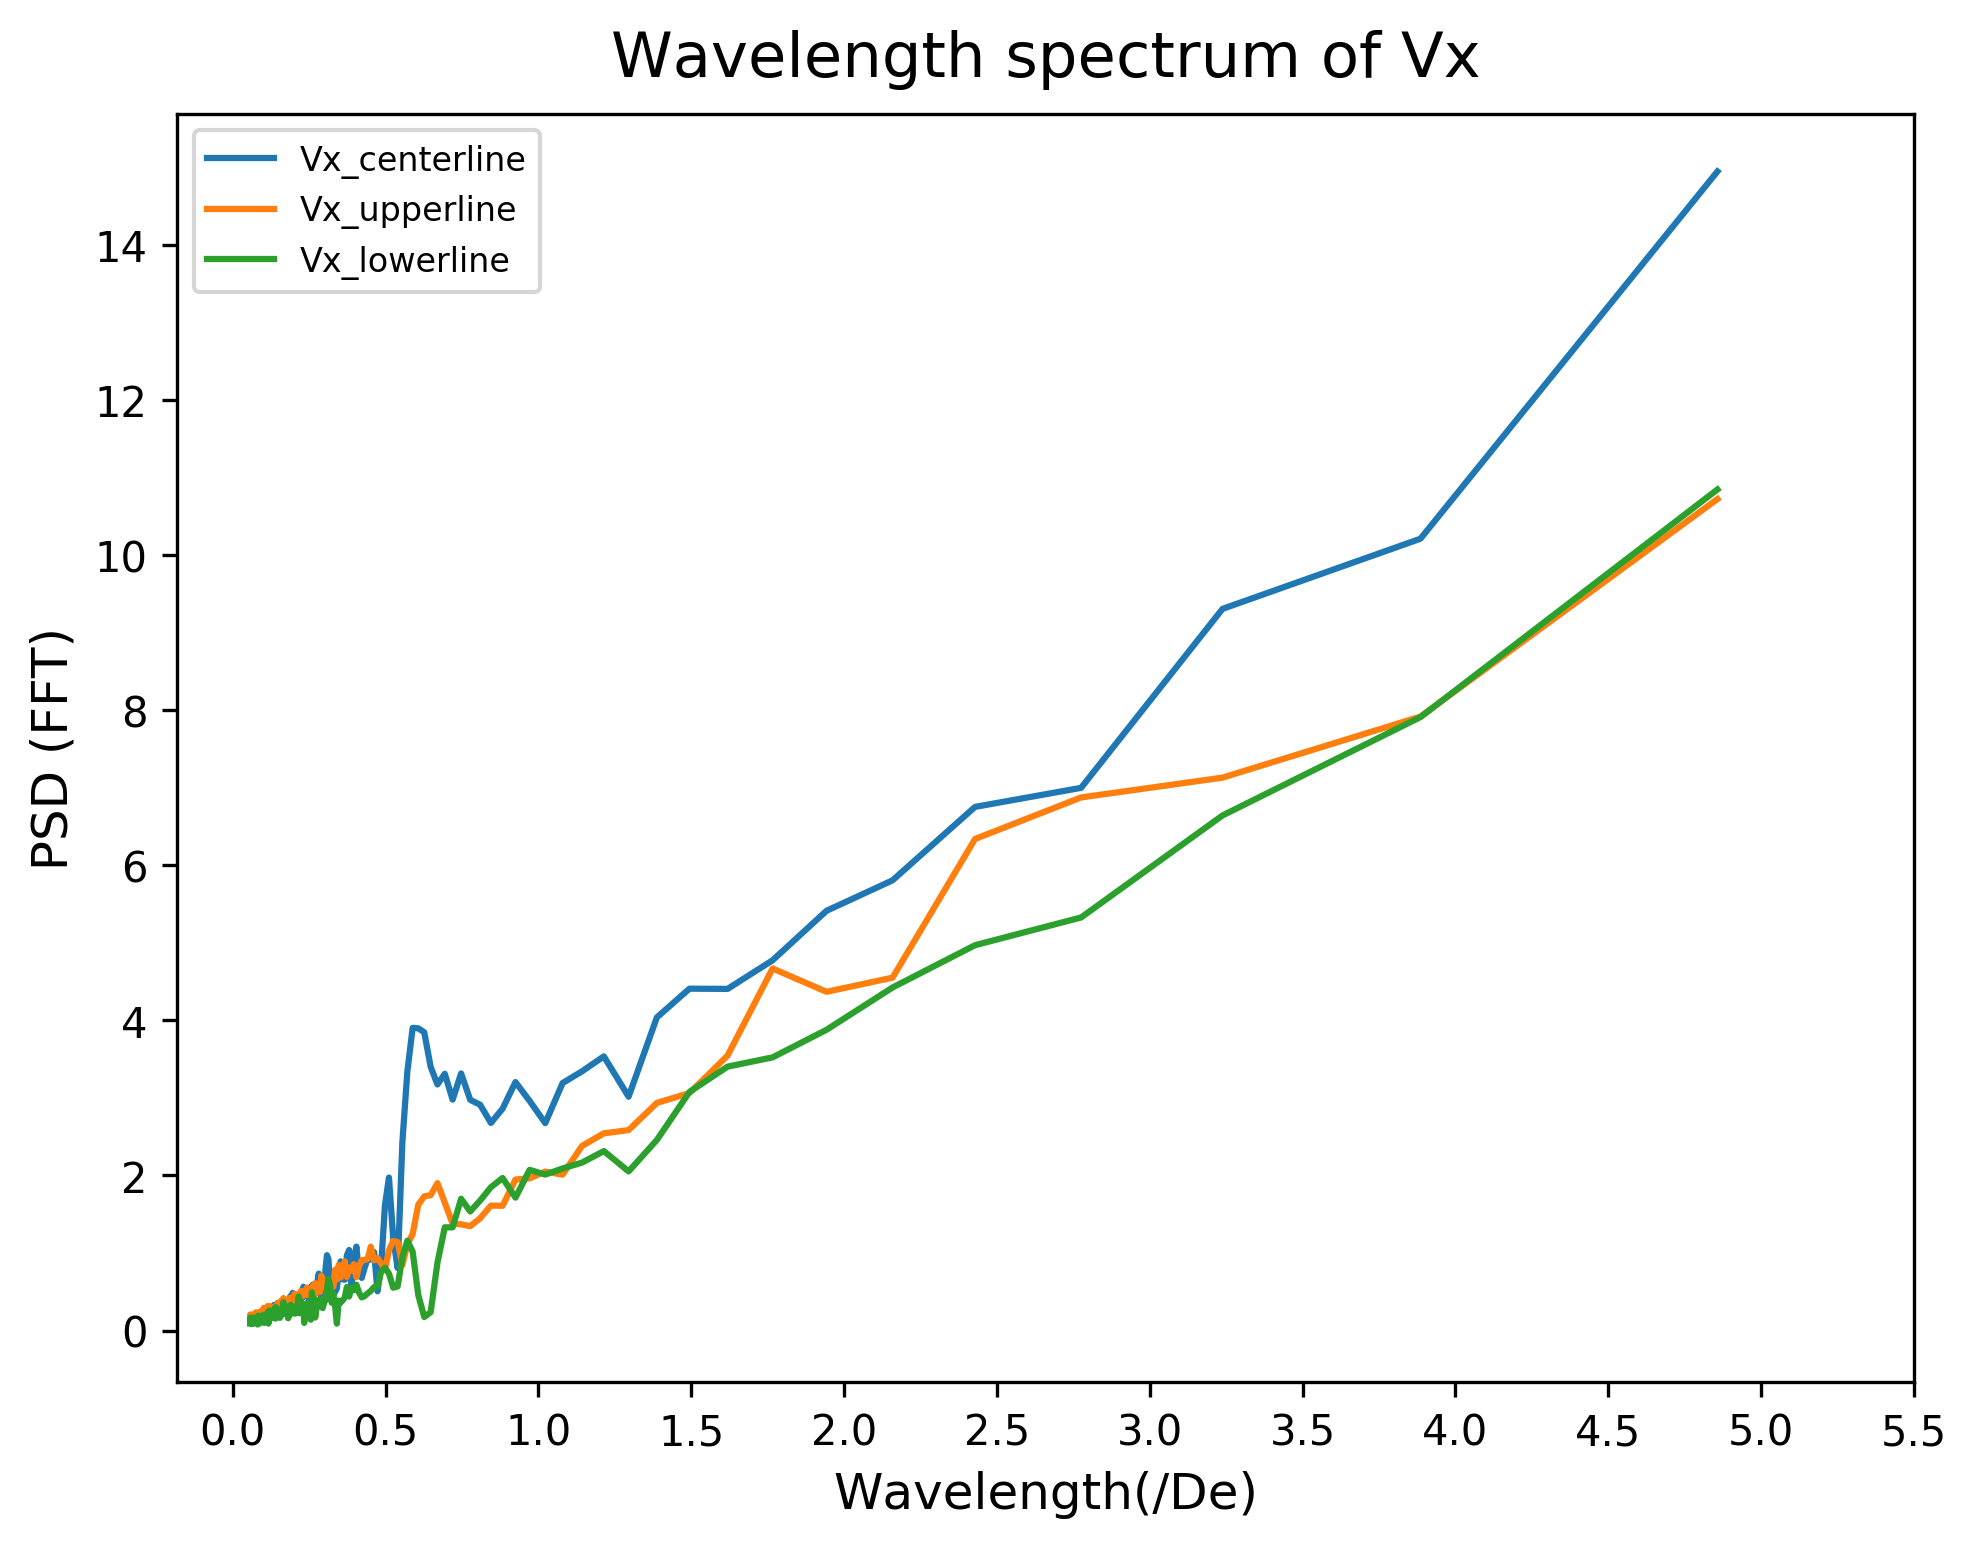
\includegraphics[width=2.5in]{images/Fft_Vx_NTR1p5_NPR2p5.png}
	\caption{NTR:1p5 NPR:2p5 }
	\label{fig:fftplots1p52p5}
\end{subfigure}%
\begin{subfigure}{.5\textwidth}
	\centering
	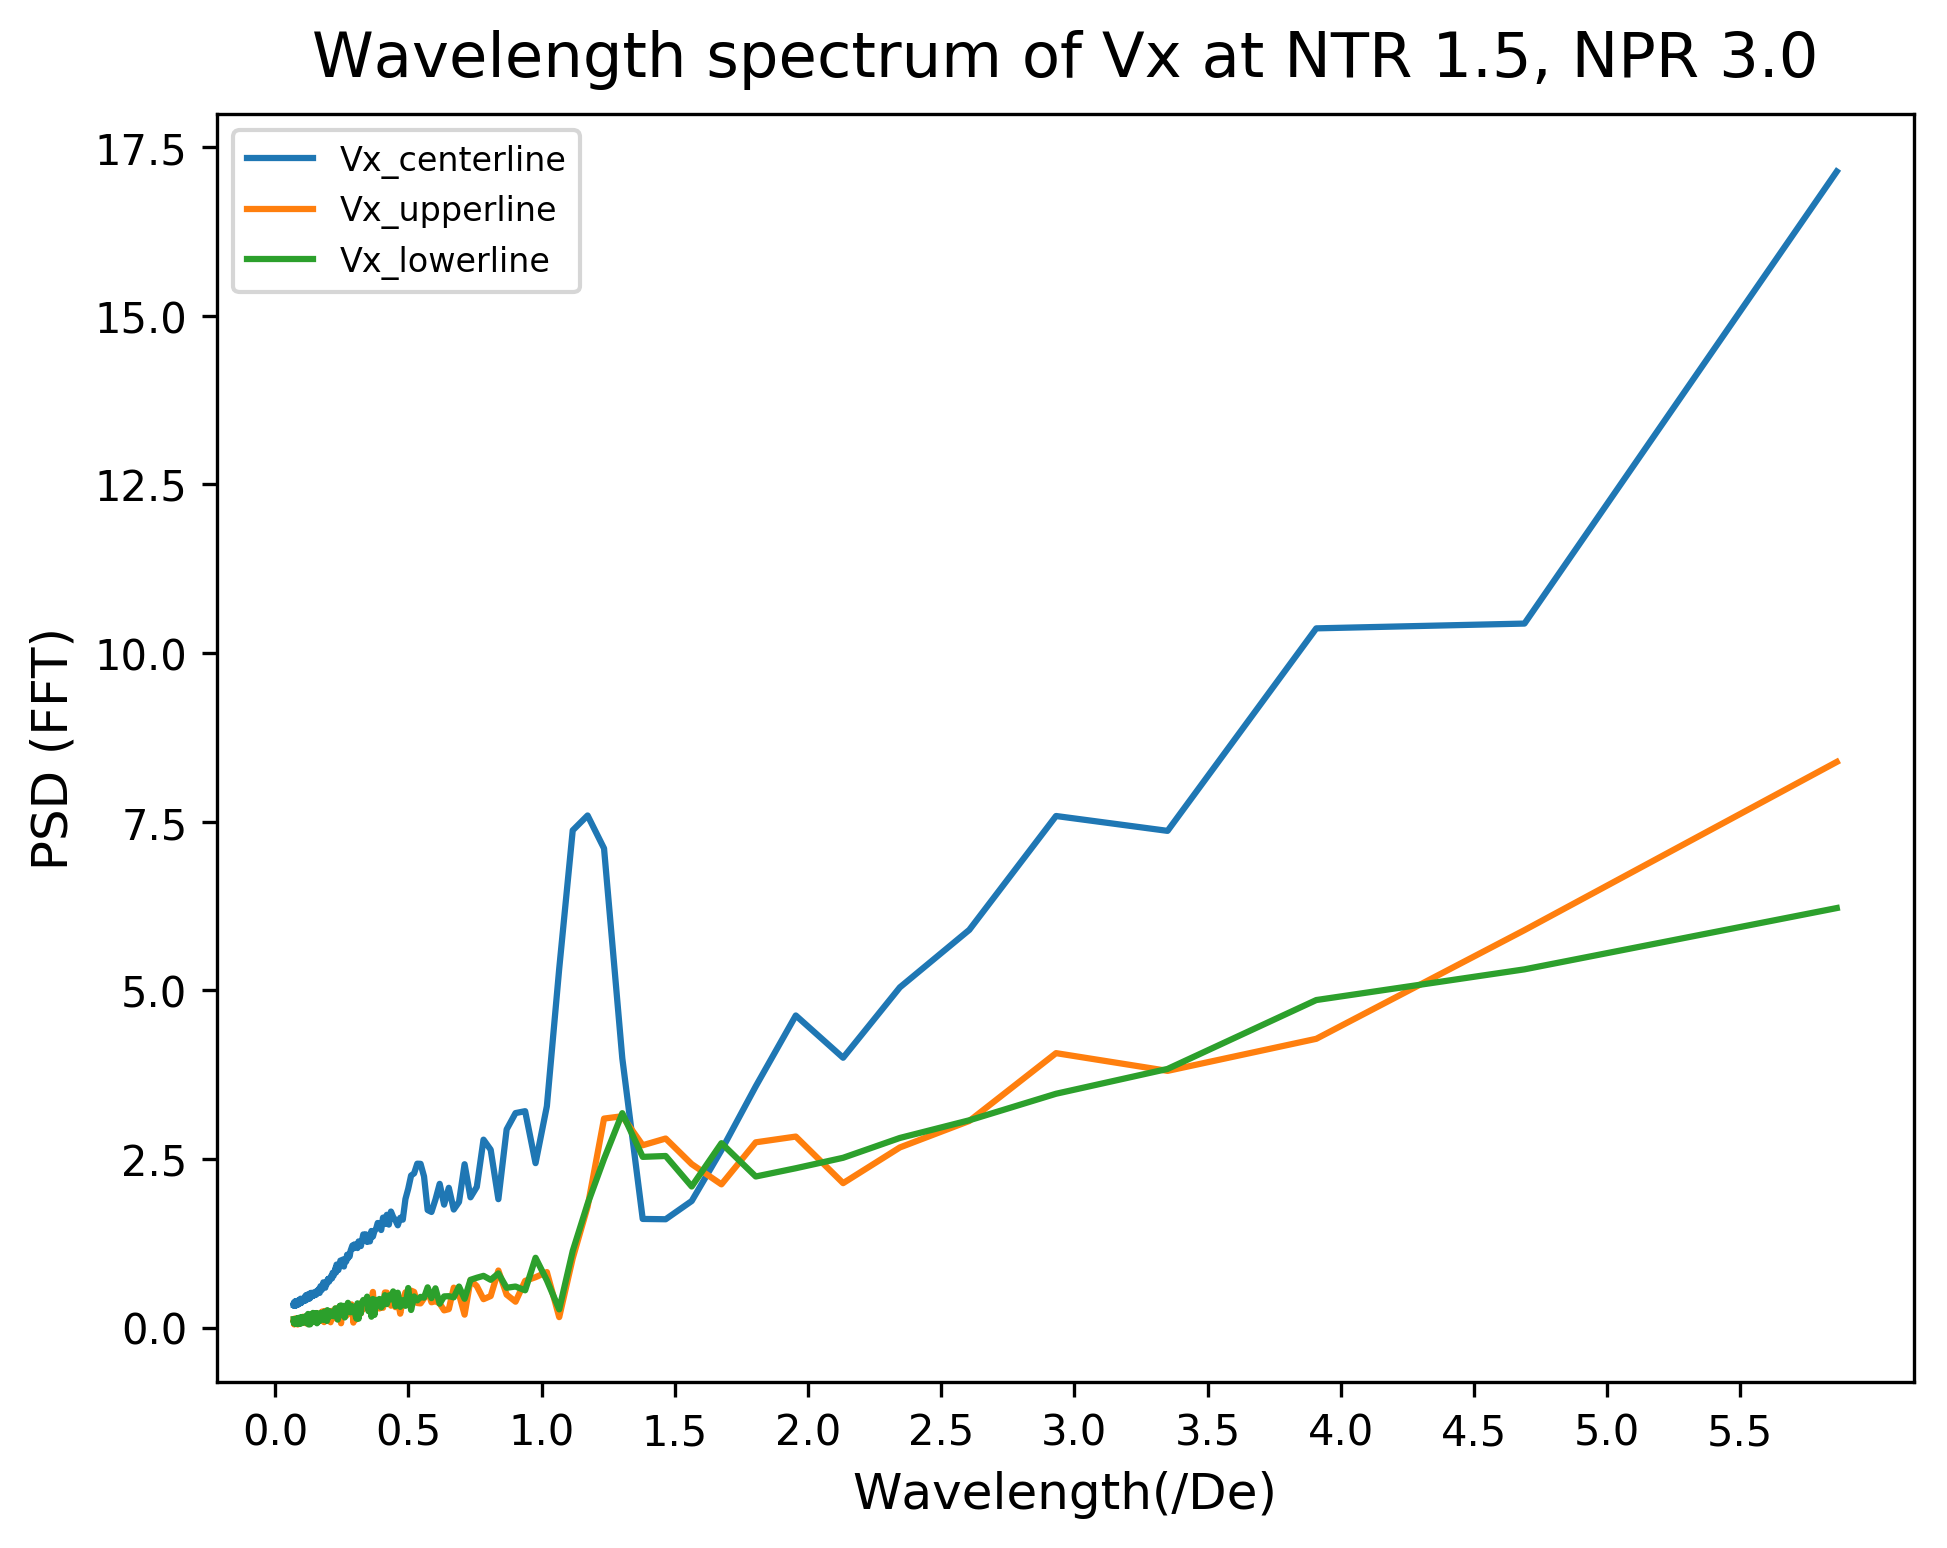
\includegraphics[width=2.5in]{images/Fft_Vx_NTR1p5_NPR3p0.png}
	\caption{NTR:1p5 NPR:3p0 }
	\label{fig:fftplots1p53p0}
\end{subfigure}
\begin{subfigure}{0.5\textwidth}
	\centering
	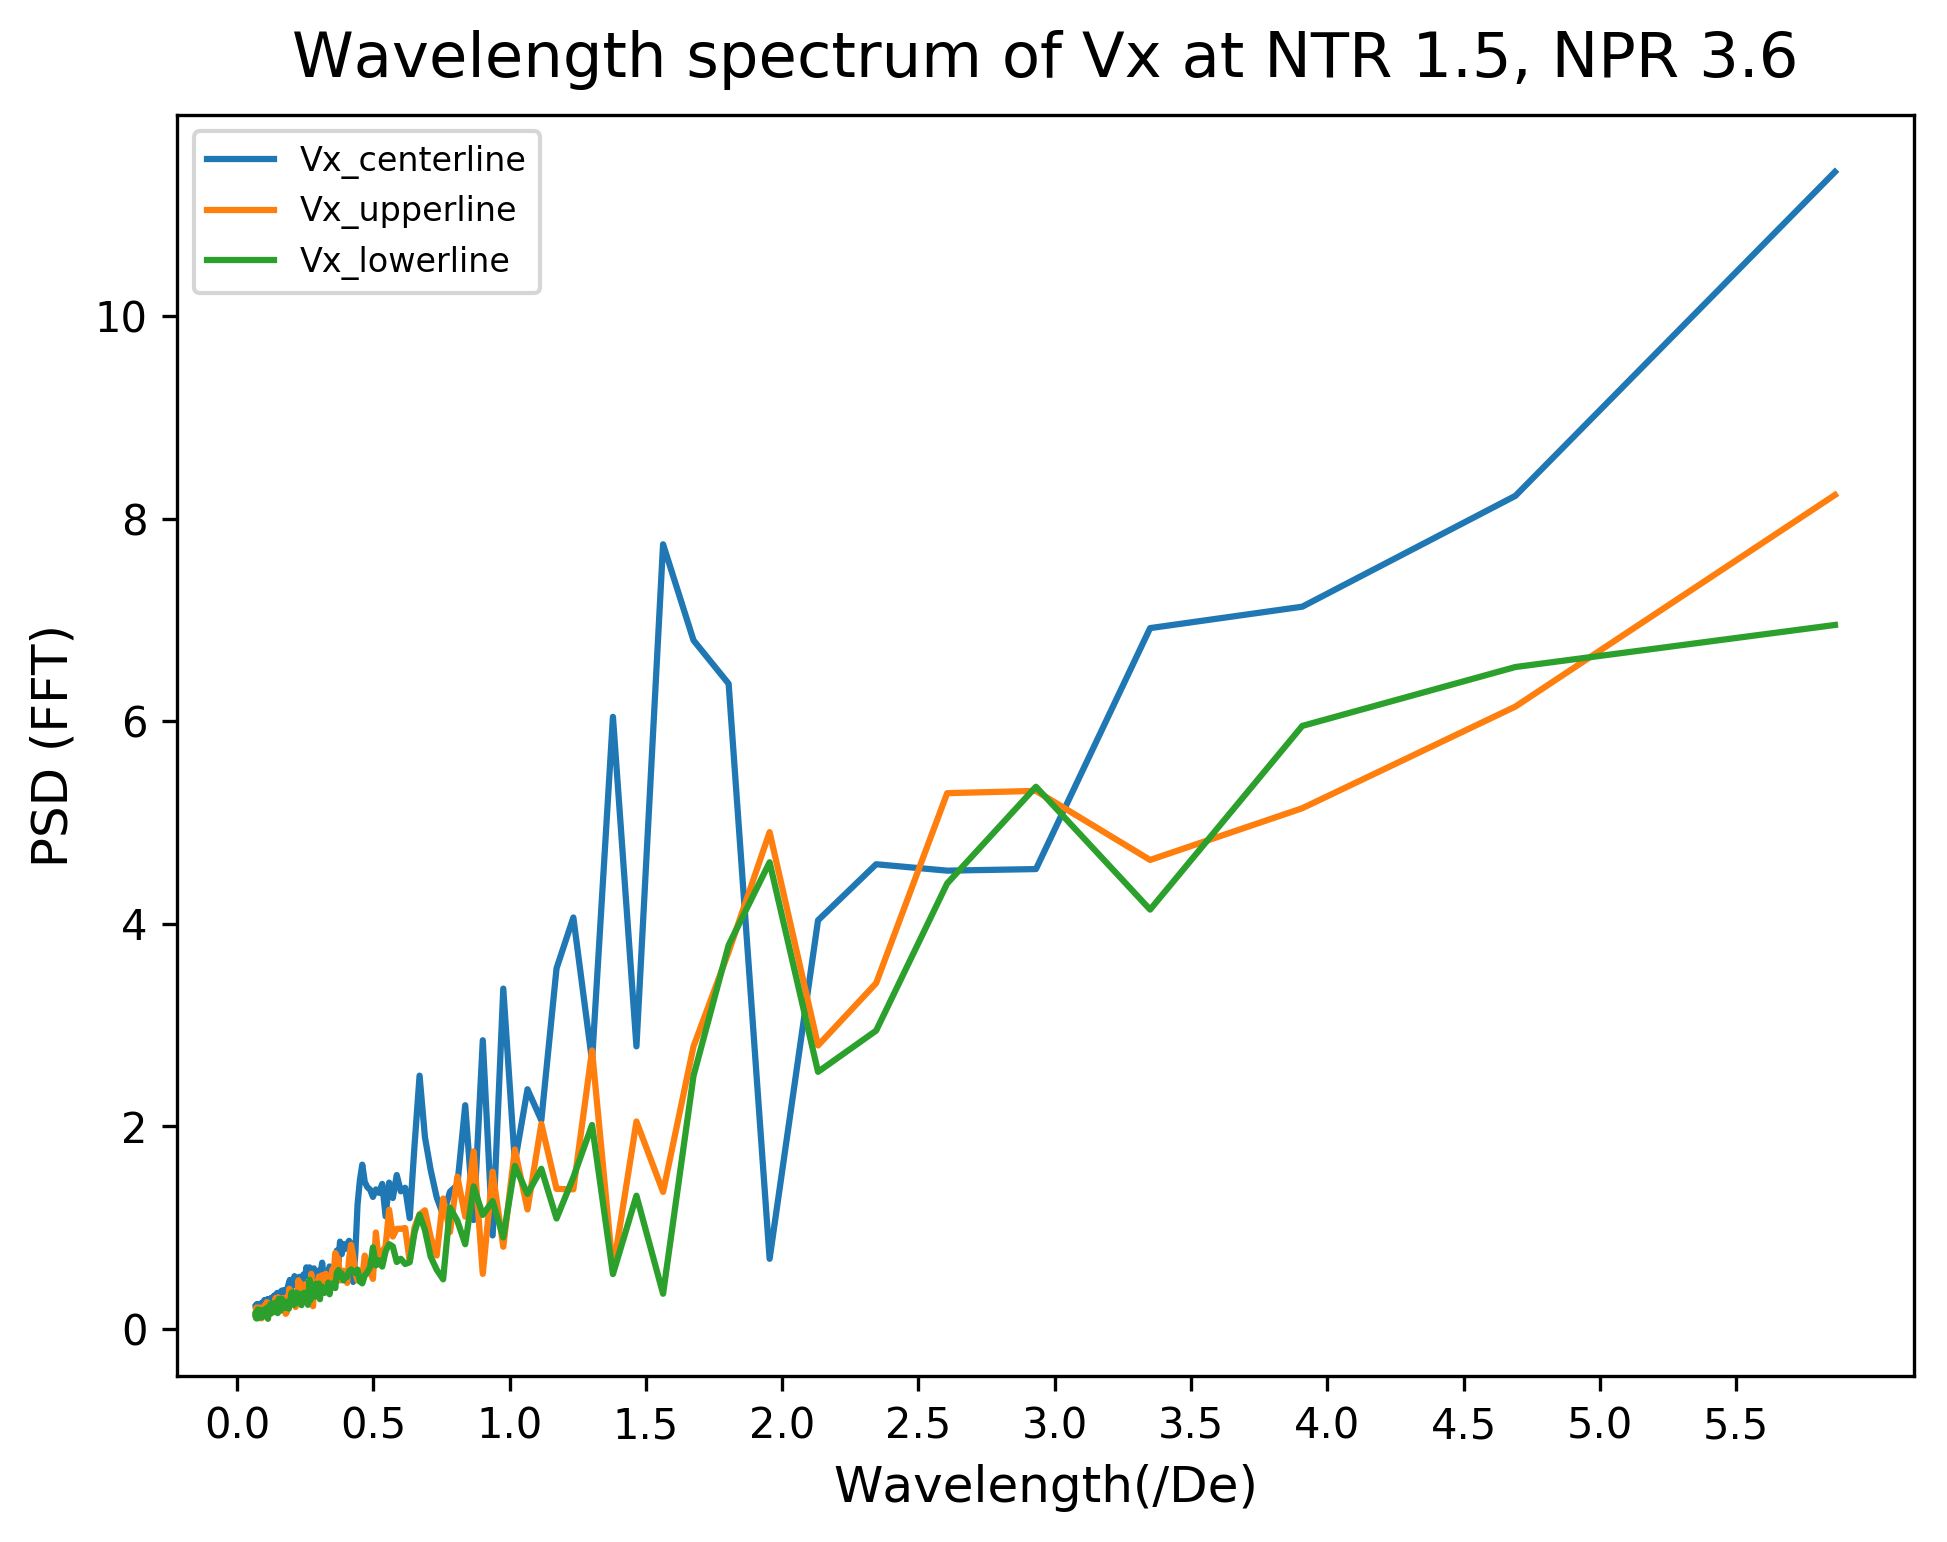
\includegraphics[width=2.5in]{images/Fft_Vx_NTR1p5_NPR3p6.png}
	\caption{NTR:1p5 NPR:3p6 }
	\label{fig:fftplots1p53p6}
\end{subfigure}
\begin{subfigure}{0.5\textwidth}
	\centering
	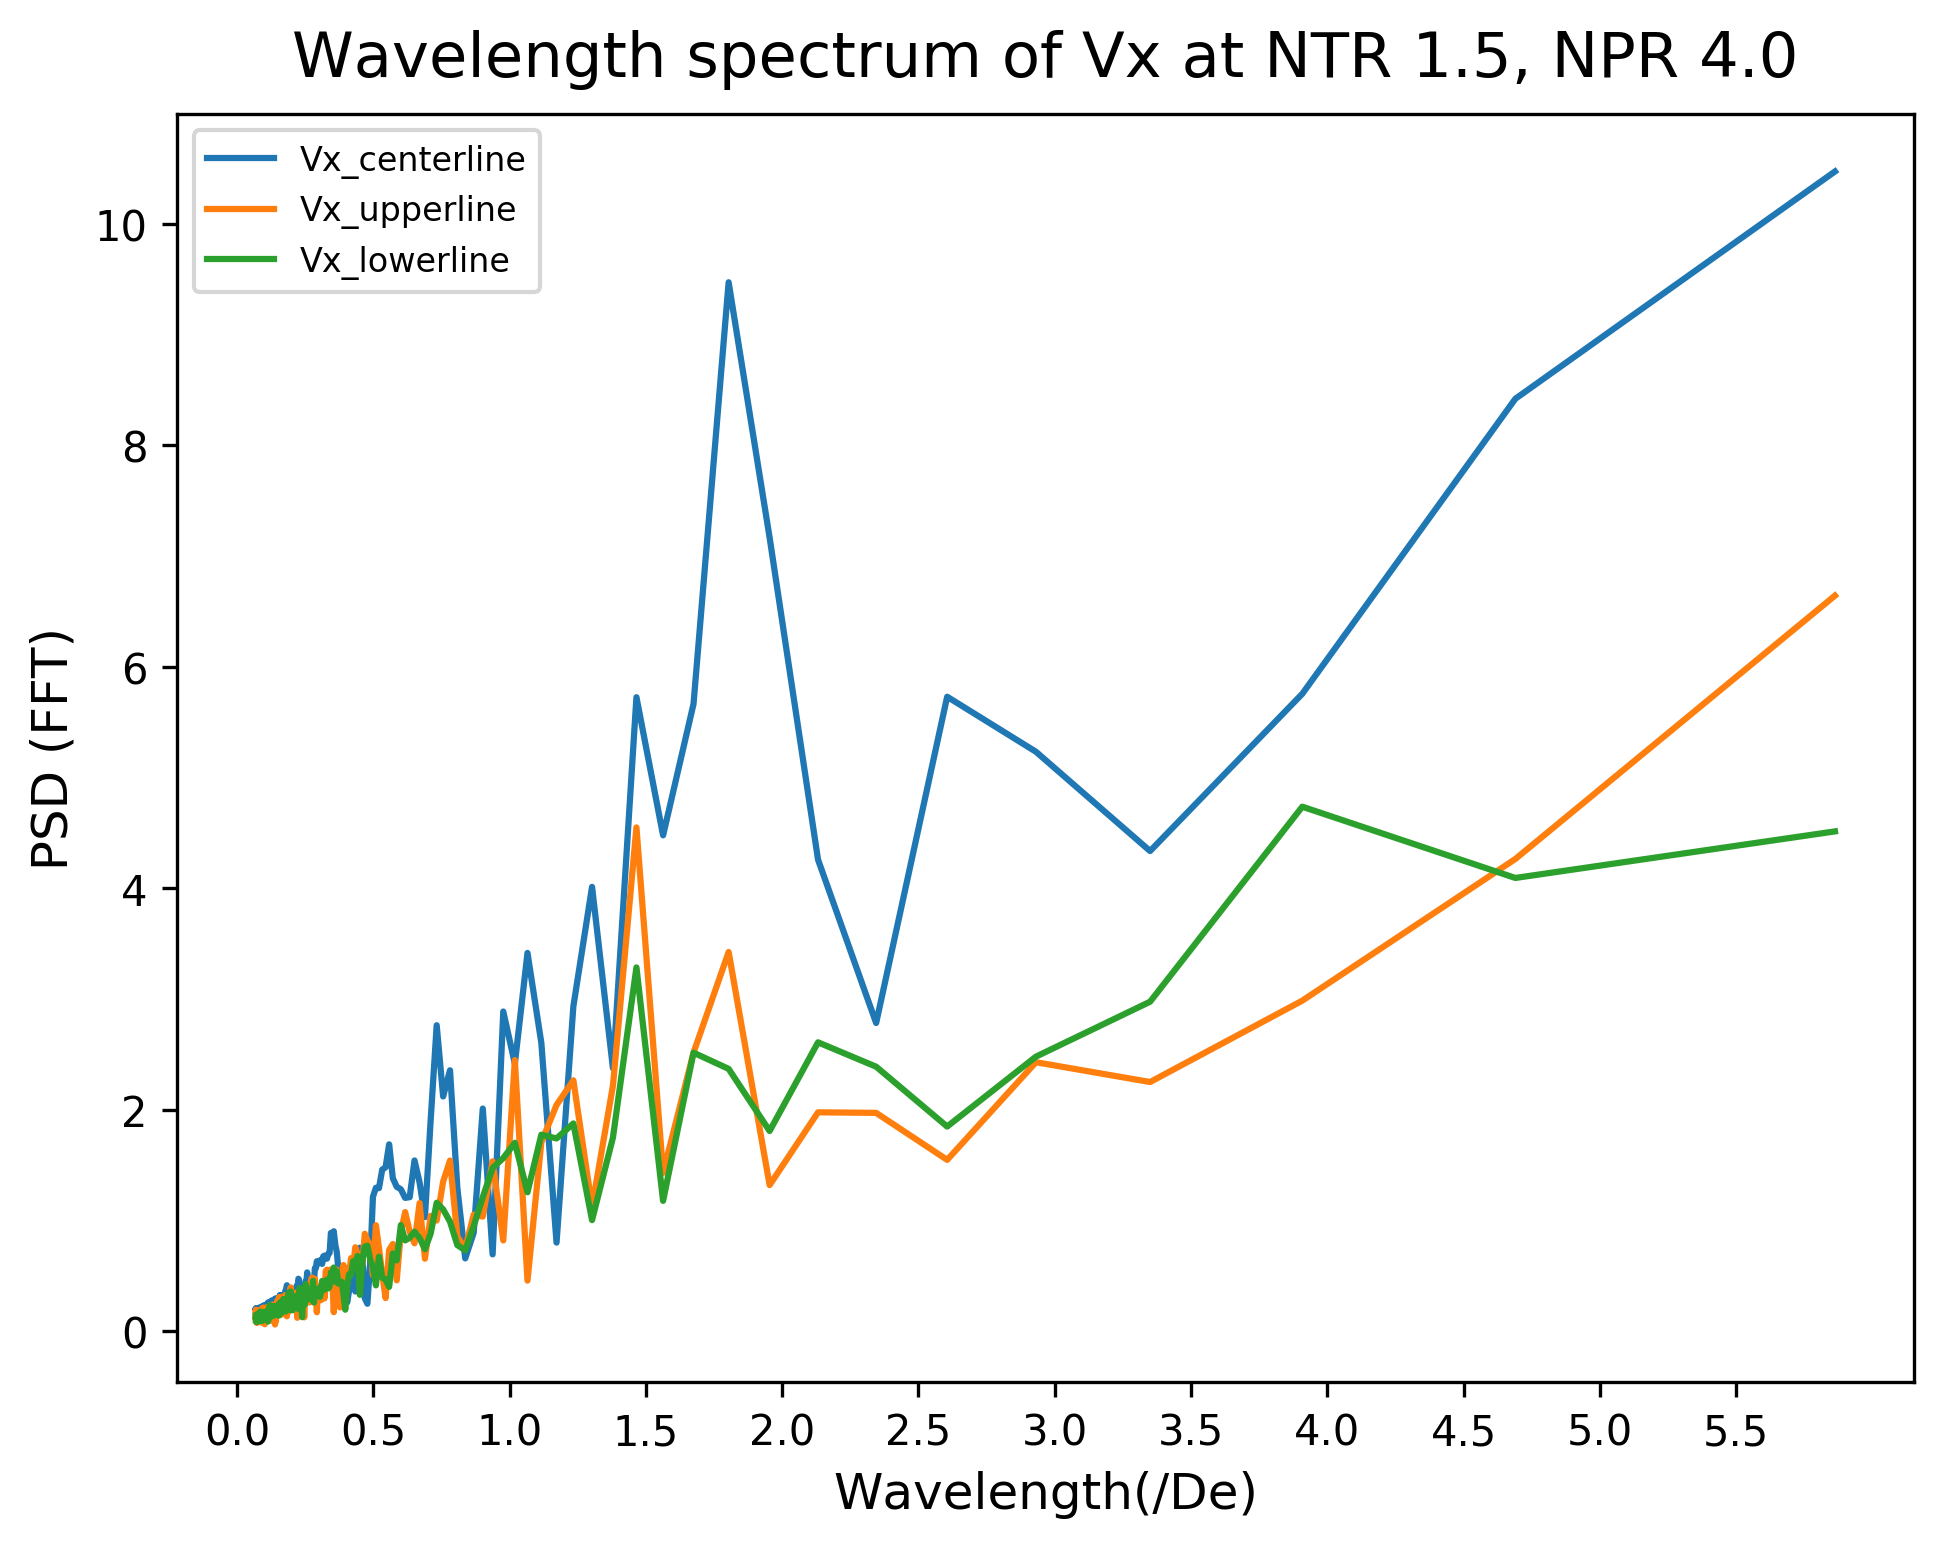
\includegraphics[width=2.5in]{images/Fft_Vx_NTR1p5_NPR4p0.png}
	\caption{NTR:1p5 NPR:4p0 }
	\label{fig:fftplots1p54p0}
\end{subfigure}
\begin{subfigure}{1.0\textwidth}
	\centering
	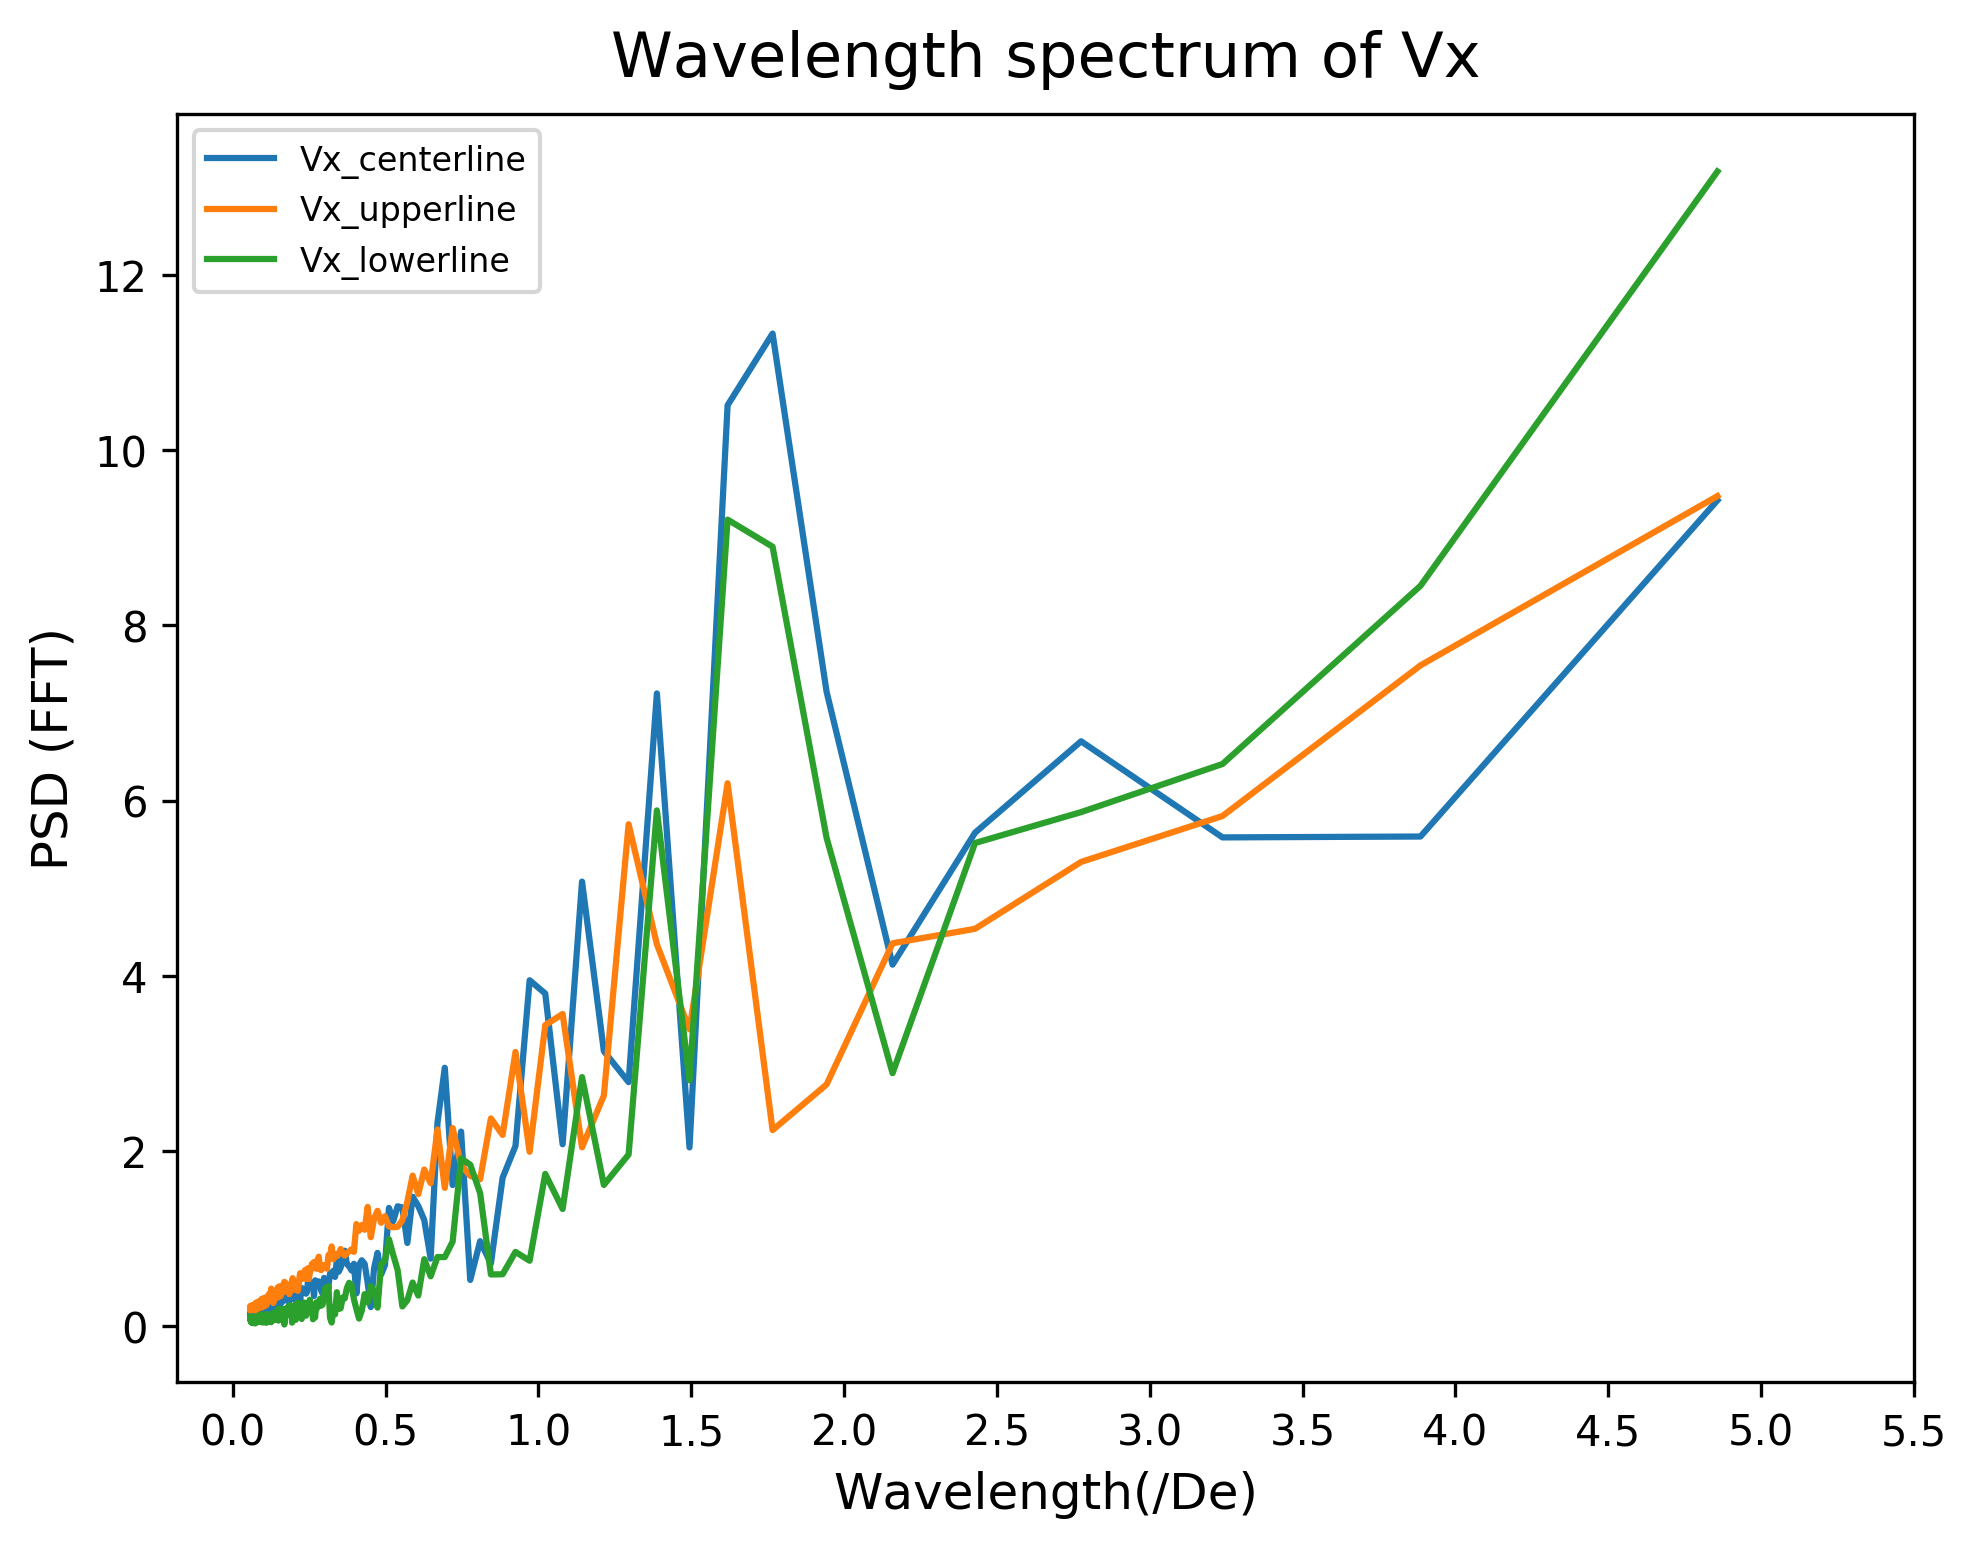
\includegraphics[width=2.5in]{images/Fft_Vx_NTR1p5_NPR4p5.png}
	\caption{NTR:1p5 NPR:4p5 }
	\label{fig:fftplots1p54p5}
\end{subfigure}
\caption{Wavelength spectrum using FFT for $V_x$ centreline data without chevrons}
\label{fig:fftplots}
\end{figure}

As we see in the FFT plots (fig \ref{fig:fftplots}), for ideally expanded flow, shock cell wavelength is close to the value earlier calculated. As the pressure increases, wavelength with maximum psd increases.This We can notice that in 2d plots too(fig \ref{fig:2dplots}). But the huge change in shock cell length from underexpanded to overexpanded can not be explained by the Tam's equation since change in $D_j$ is small relatively. This shows that the equation, as it is, has limitations in the range of its application.  It is also interesting to note that the wavelengths are well defined for underexpanded flows because of the few oblique shocks. For overexpanded flows, since the shocks are due to the large number of reflected expansion waves, the wavelength pattern is more rugged. So is the case for near perfectly expanded flow.\\

Inlet temperature doesn't seem to have major effect on wavelength pattern. Although when the NTR is 3.0, wavelength is clearly subdued. This shows that the shocks are not as intense as of colder flows \\

\section{Merging of shocks and shear layers}
If we carefully observe in the fig \ref{fig:2dplots}, two shocks exist at the lip forming double delta pattern which merge later in the jet wake. Although NPR was close to perfect expansion which should give only shocks reflected inside the nozzle, imperfections in equipment might be the reason for multiple shock structures. TKE at the lips seems to be highest, which shows the importance of screech tone generation. It is easier to notice the shocks merging in lineplots of $V_x$ (fig \ref{fig:lineplotsVx}) when compared to 2D plots. Shocks originated before jet exit seem to run slower than the ones generated after, finally merging with the shear layer shocks.\\ 
 
\begin{figure}[H]
\begin{subfigure}{.5\textwidth}
	\centering
	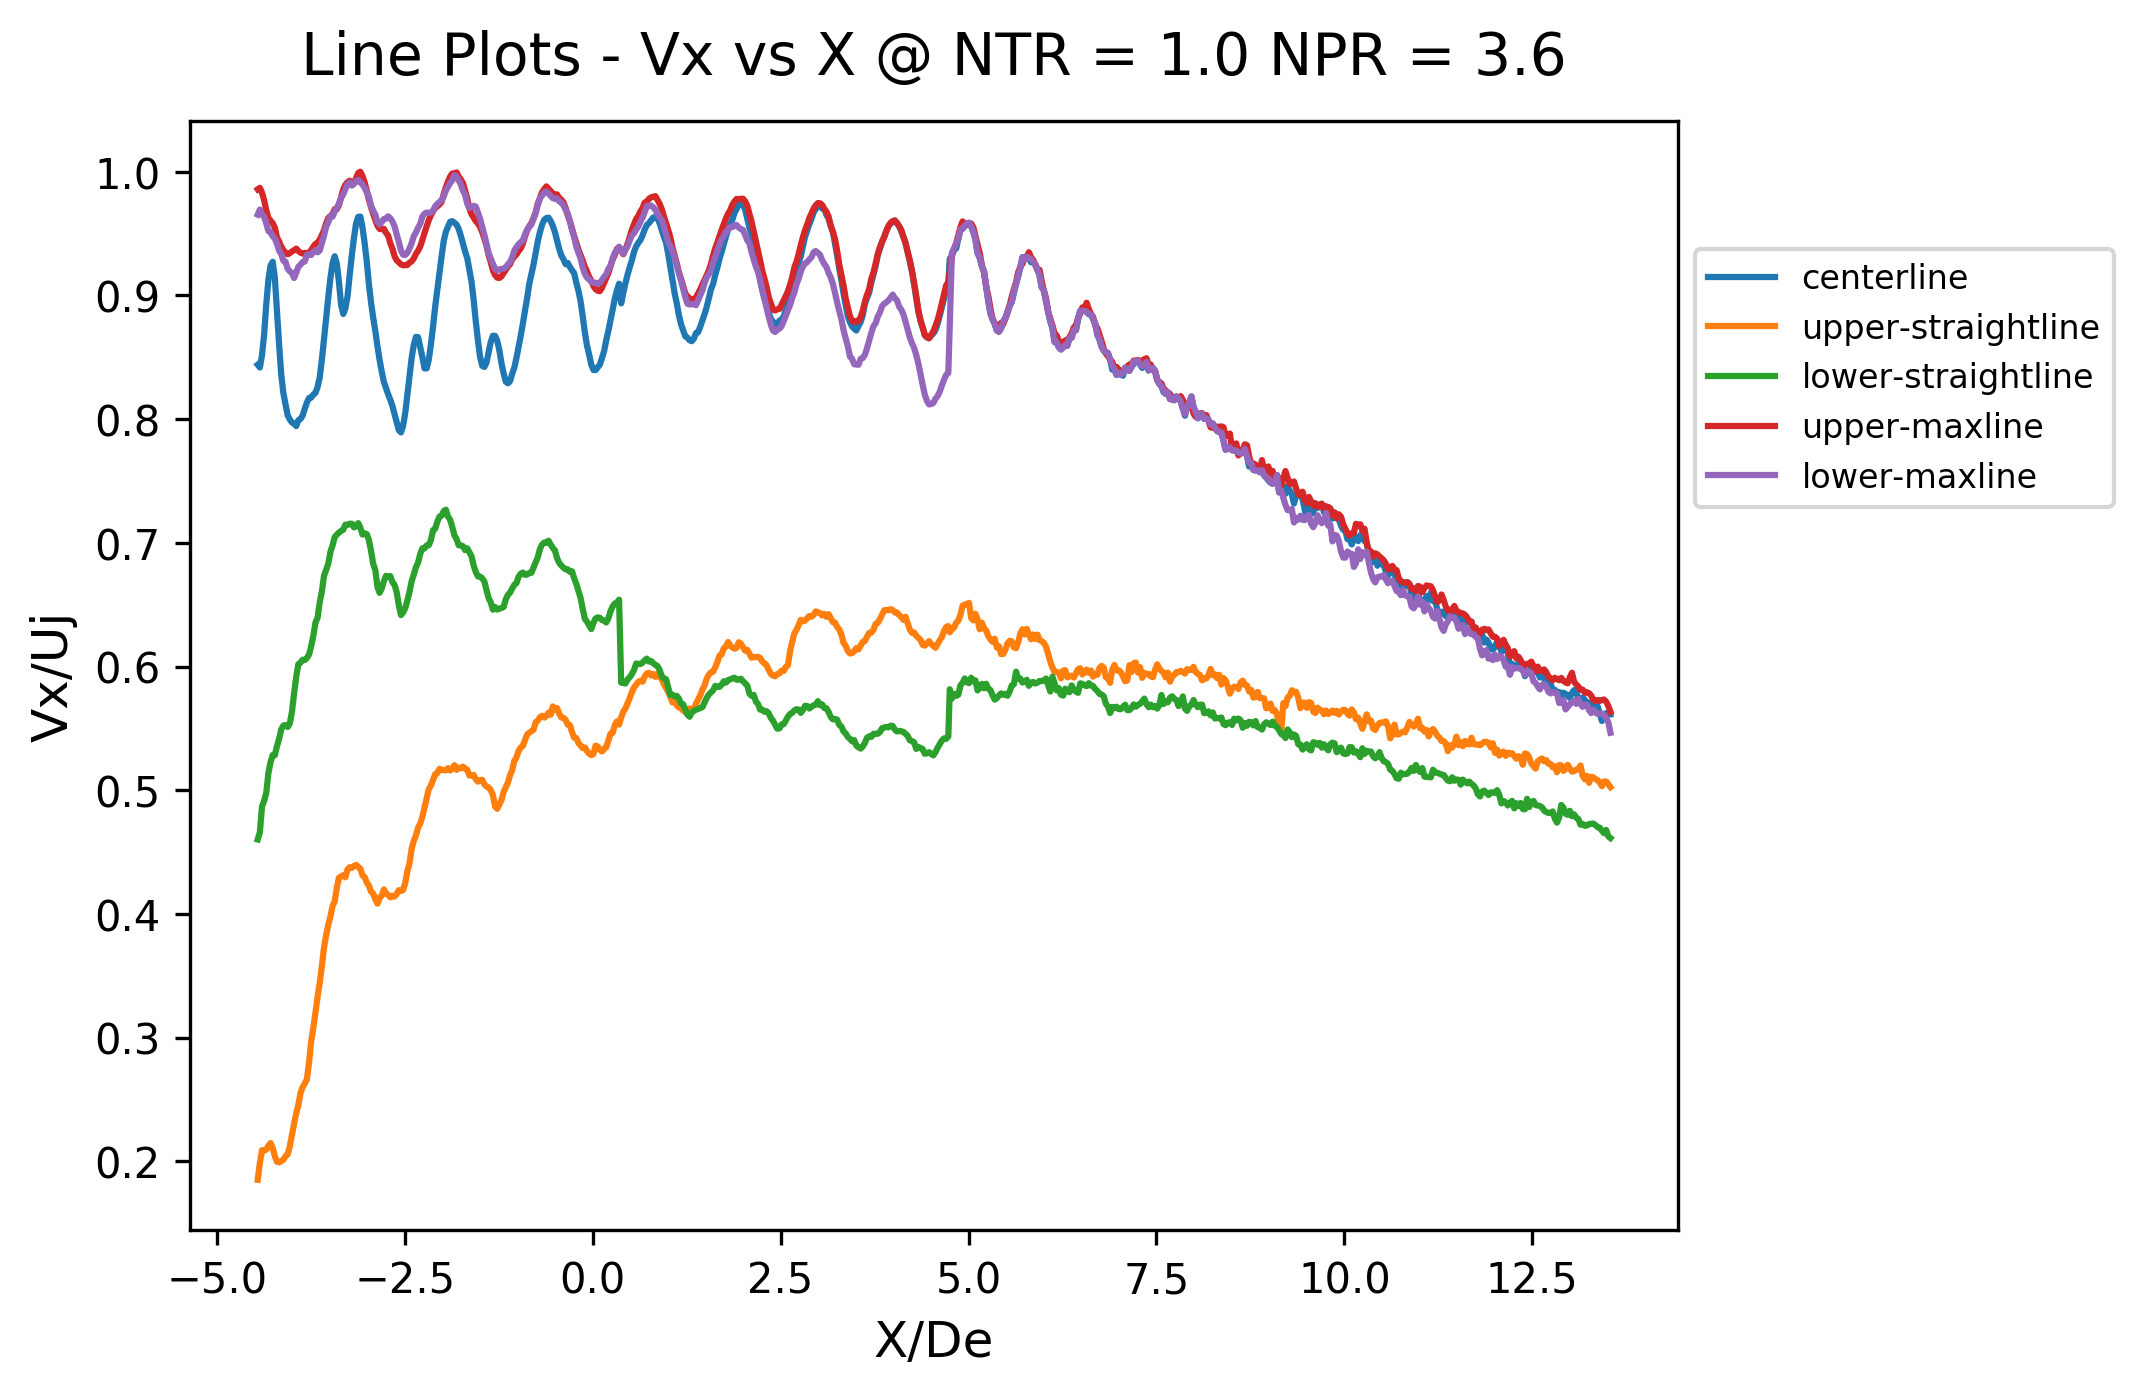
\includegraphics[width=3in]{images/LinePlots_Vx_NTR1p0_NPR3p6.png}
	\caption{NTR:1p0 NPR:3p6 }
	\label{fig:lineplotsVx1p03p6}
\end{subfigure}%
\begin{subfigure}{.5\textwidth}
	\centering
	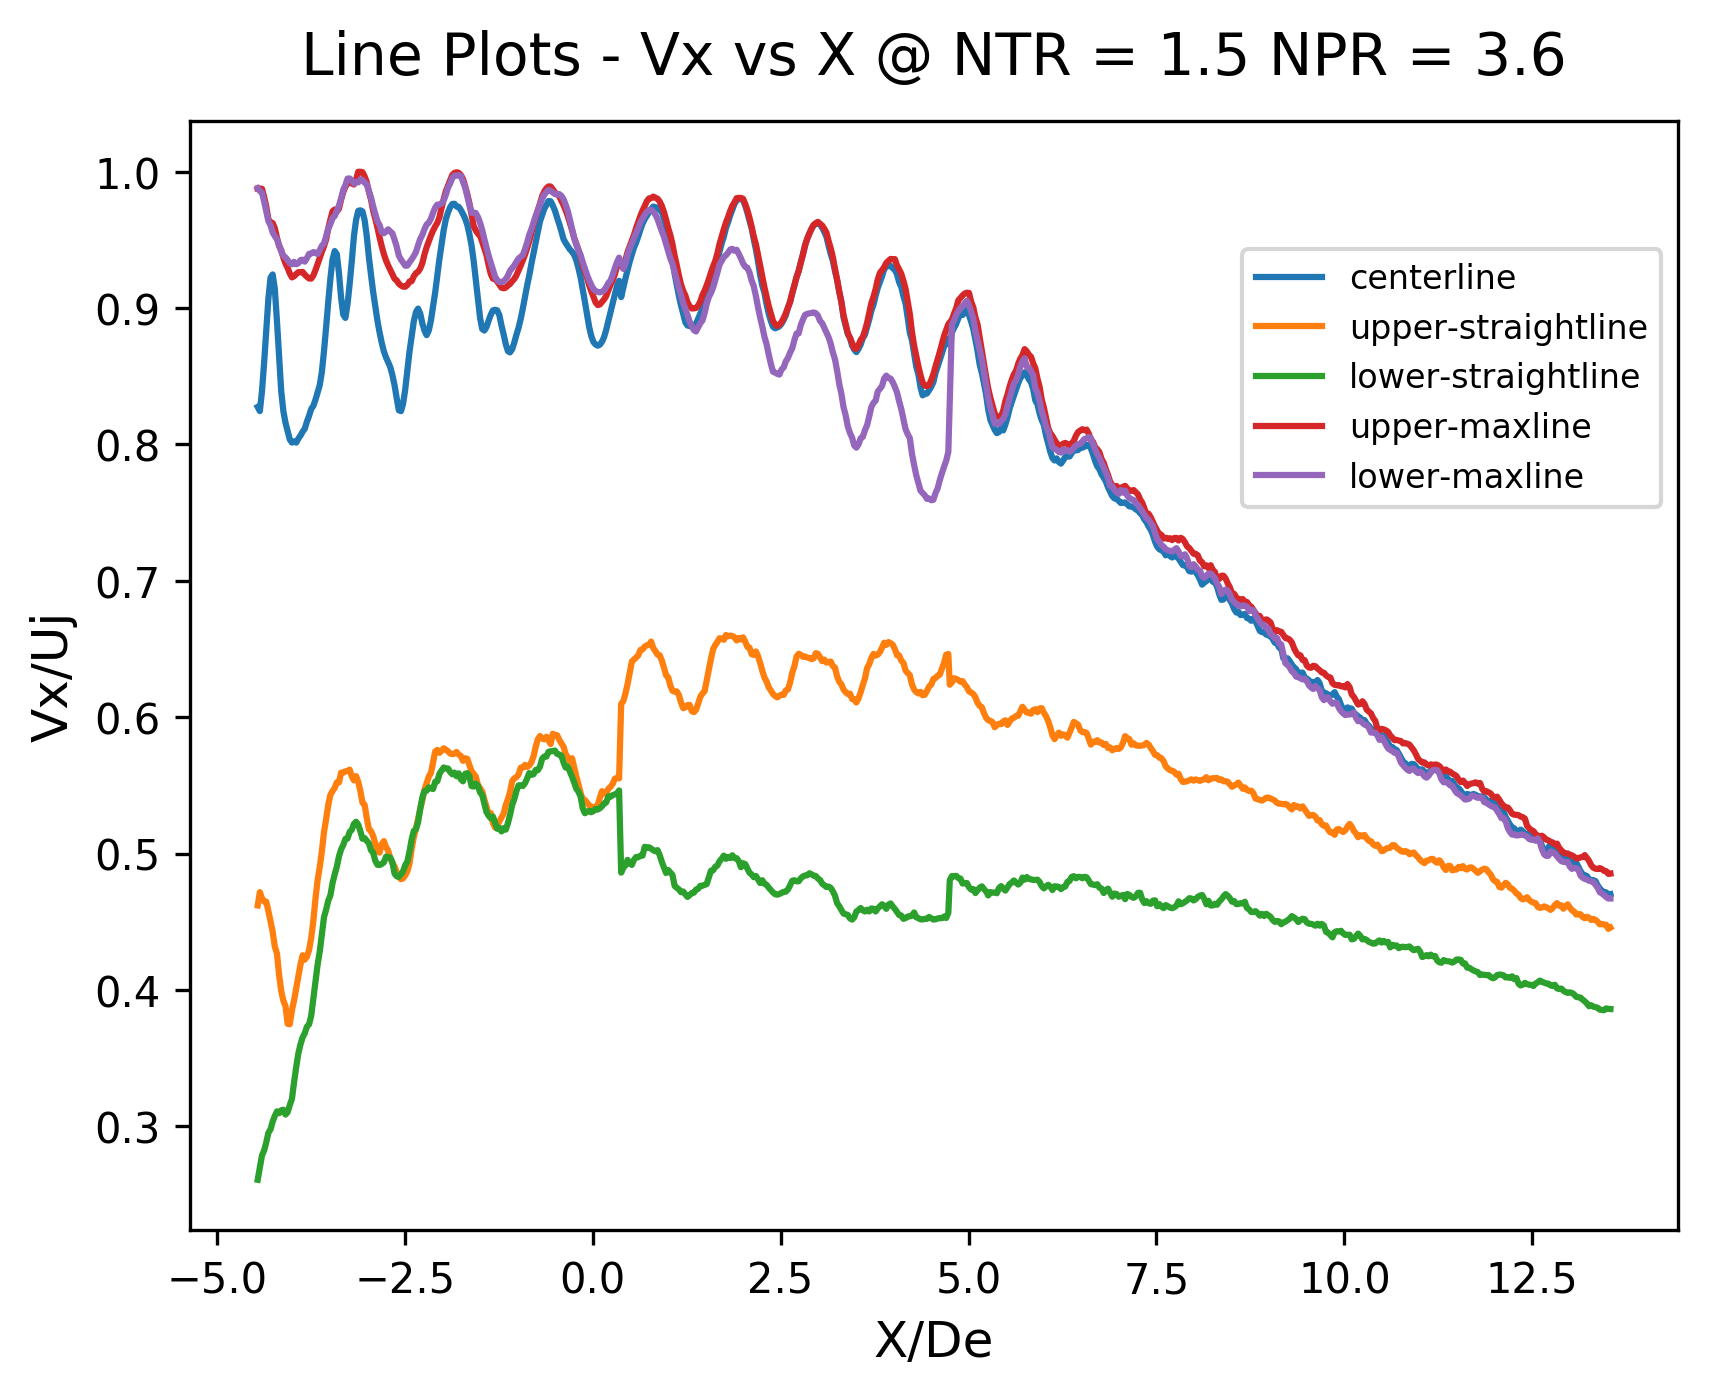
\includegraphics[width=2.5in]{images/LinePlots_Vx_NTR1p5_NPR3p6.png}
	\caption{NTR:1p5 NPR:3p6 }
	\label{fig:lineplotsVx1p53p6}
\end{subfigure}
\caption{centreline plots for $V_x$ without chevrons }
\label{fig:lineplotsVx}
\end{figure} 

Spectograms are another way to interpret lineplots data. From fig \ref{fig:spectogramVx}, most of the spectrum seem to be around the wavenumber (1/wavelength) that we calculated analytically and also noticed in FFT plots(fig \ref{fig:fftplots}). Precision is not high as the sampling data is small, but it gives an idea of spectrum at every point along jet. Multiple wavenumbers merging to form a single broad smudge shows merging of shocks and decrease substantially showing the end of potential core because of merging of shear layers. 

\begin{figure}[H]
\begin{subfigure}{0.5\textwidth}
	\centering
	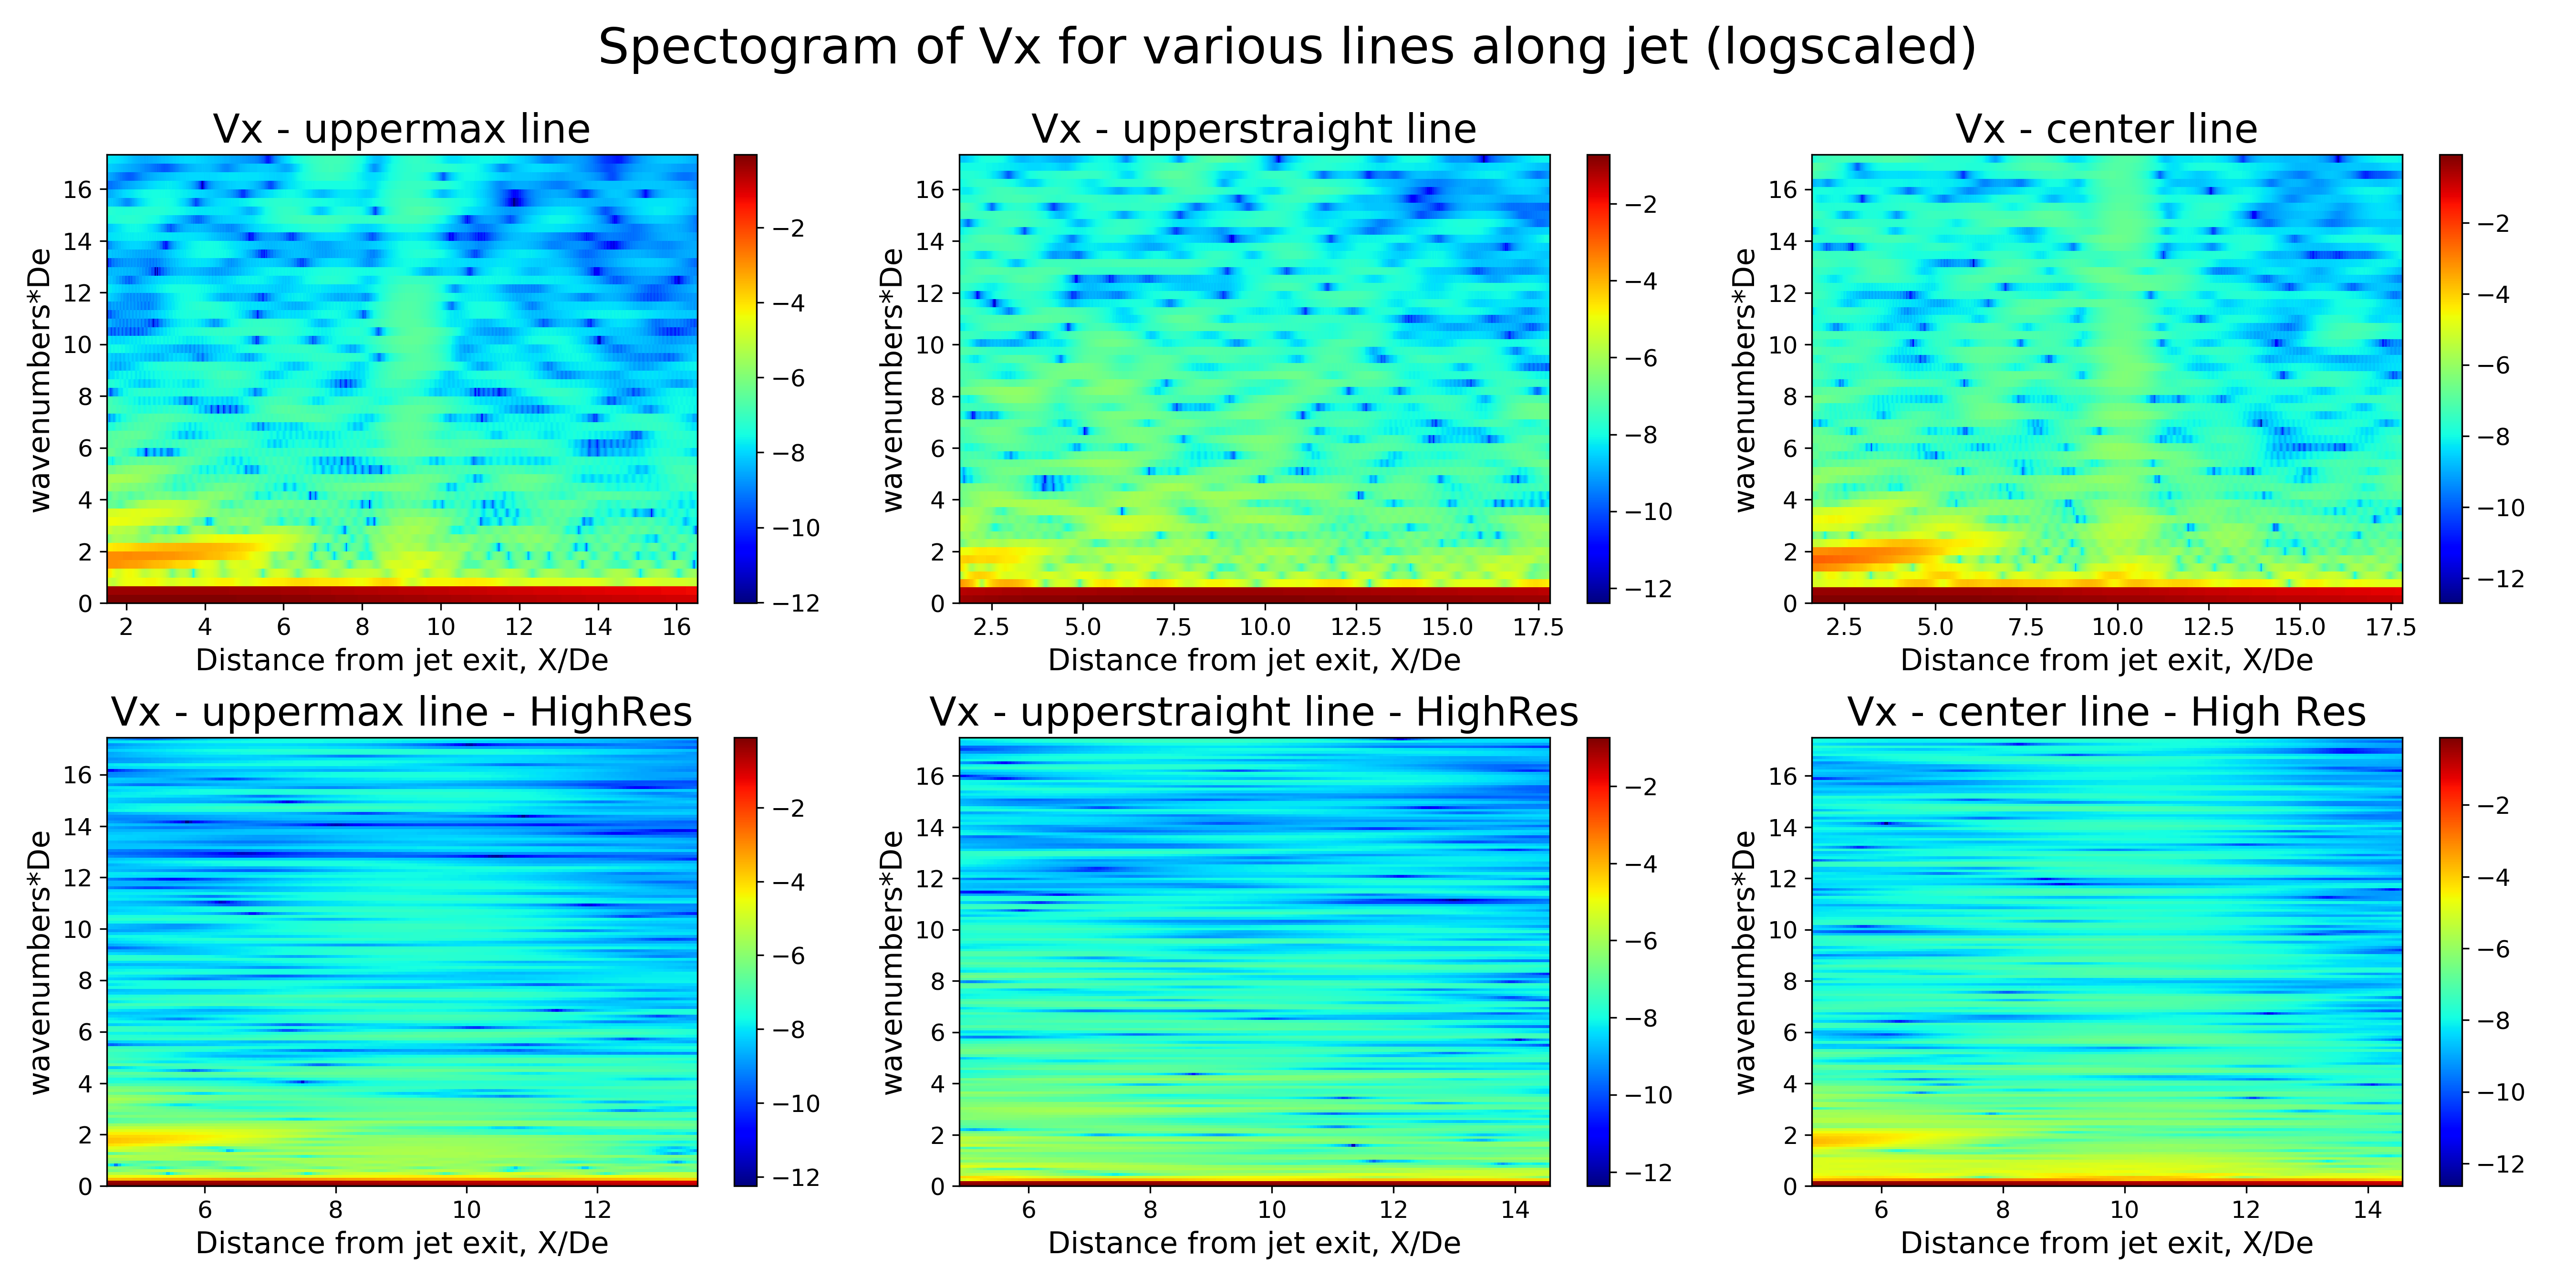
\includegraphics[width=3in]{images/Spectogram_Vx_NTR2p5_NPR2p5.png}
	\caption{NTR:2p5 NPR:2p5 }
	\label{fig:spectogramVx2p52p5}
\end{subfigure}%
\begin{subfigure}{0.5\textwidth}
	\centering
	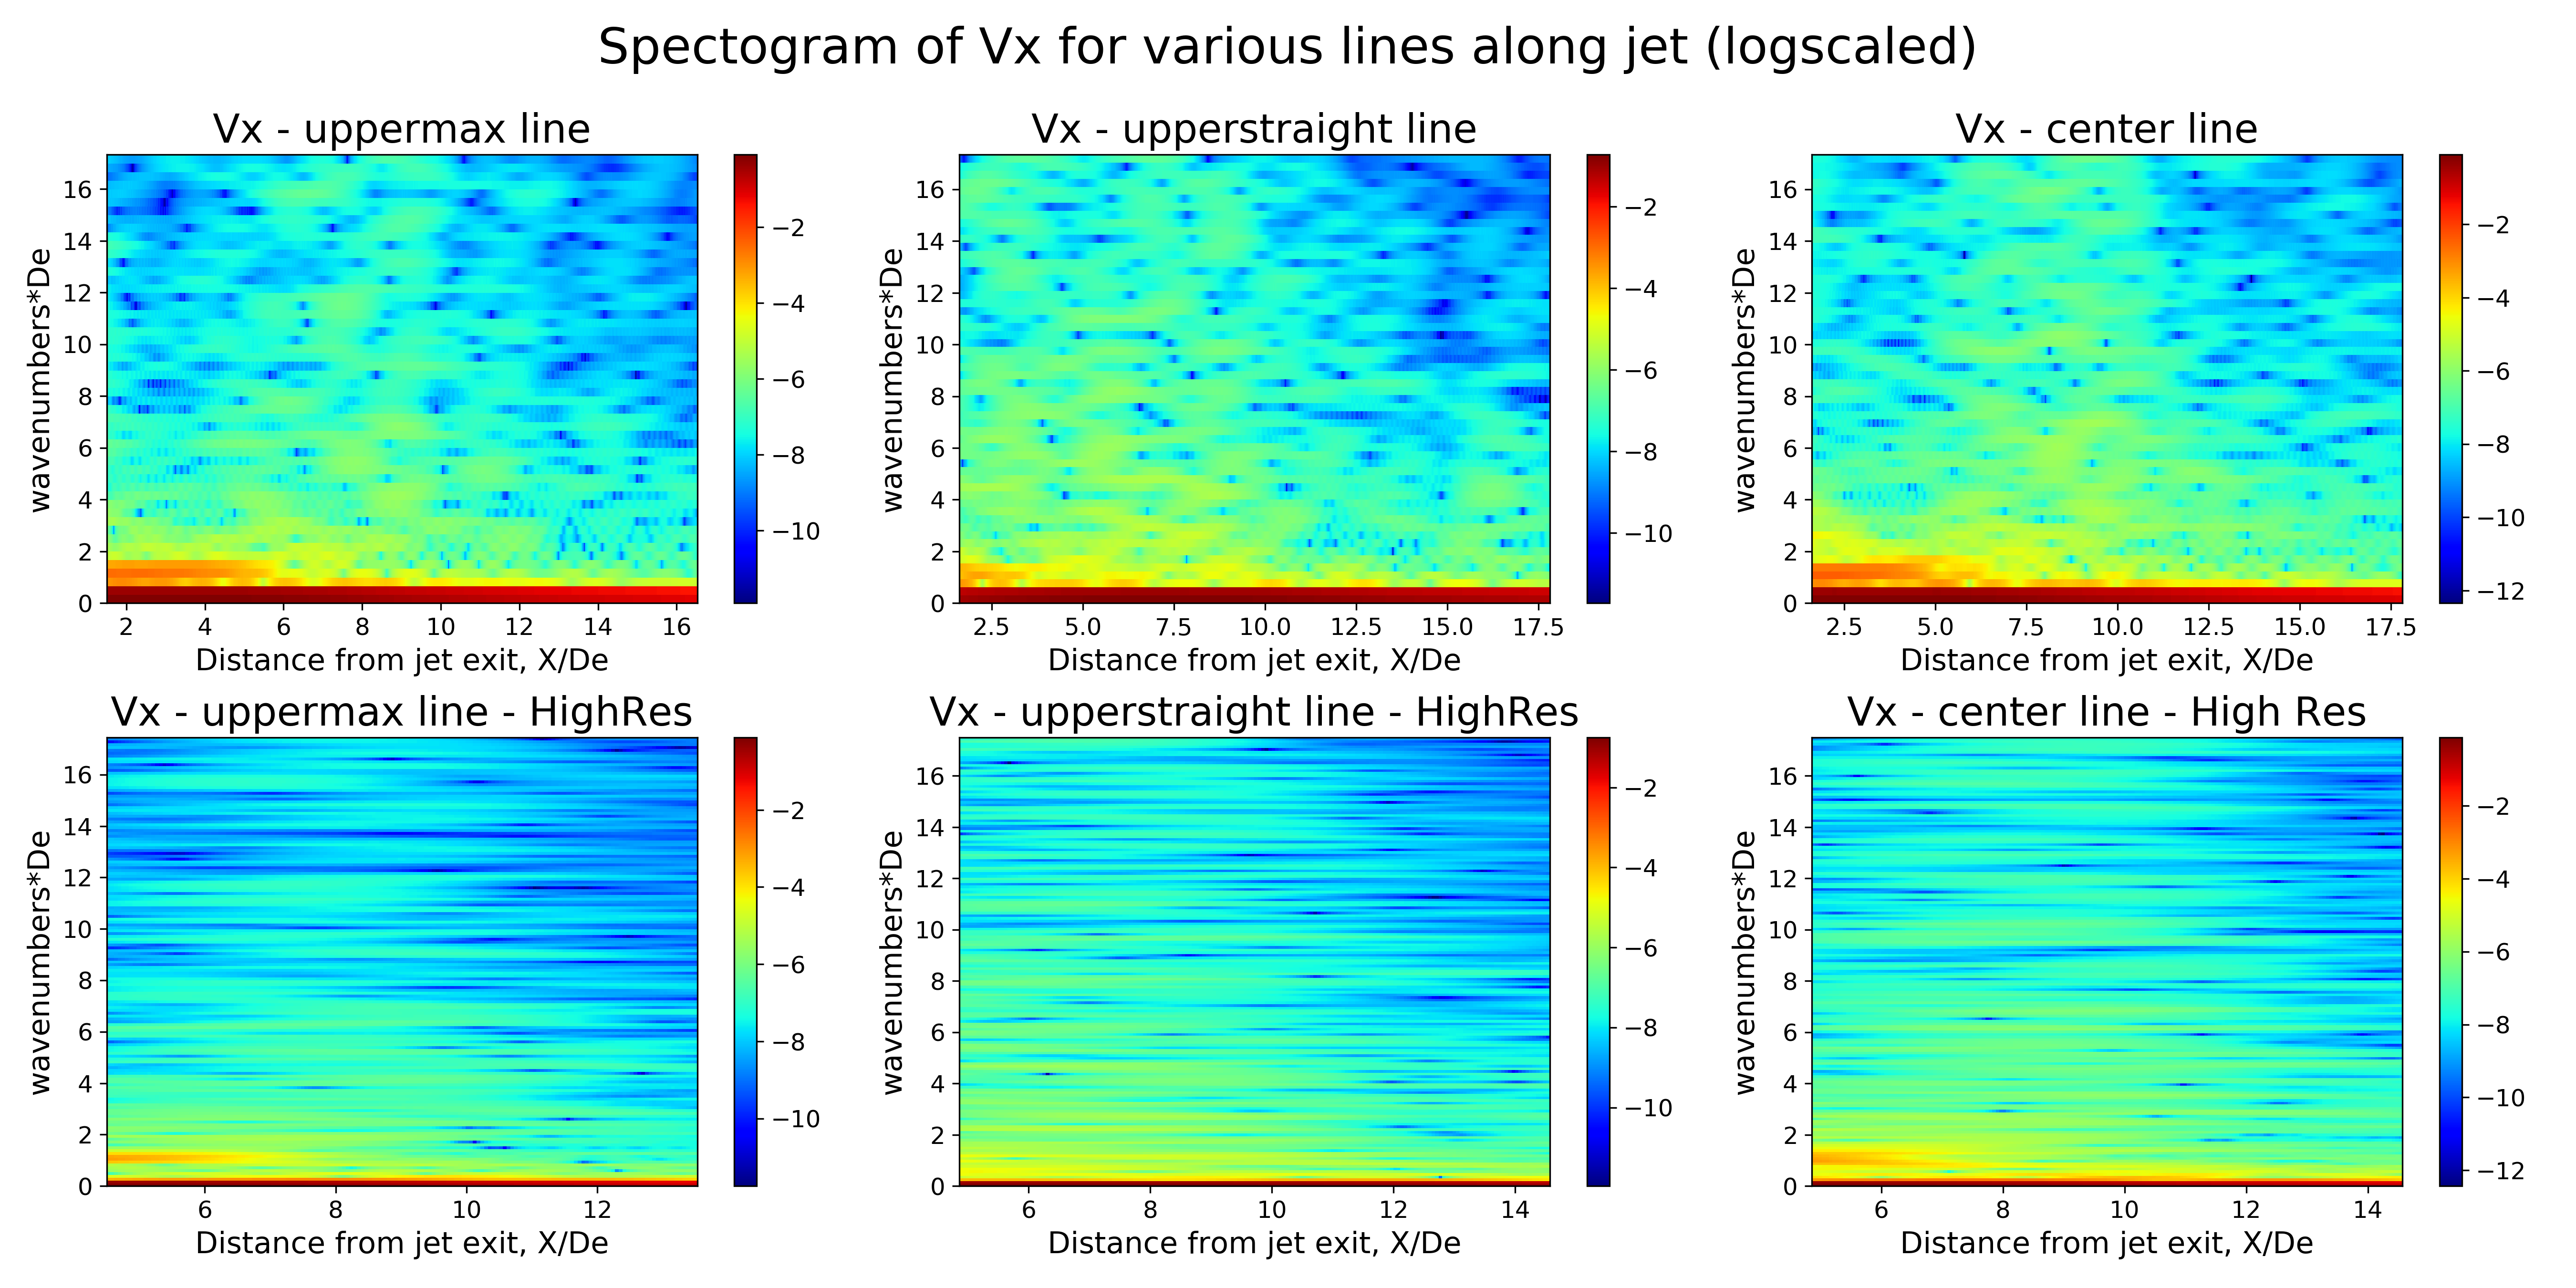
\includegraphics[width=3in]{images/Spectogram_Vx_NTR2p5_NPR3p0.png}
	\caption{NTR:2p5 NPR:3p0 }
	\label{fig:spectogramVx2p53p6}
\end{subfigure}\\
\begin{subfigure}{0.5\textwidth}
	\centering
	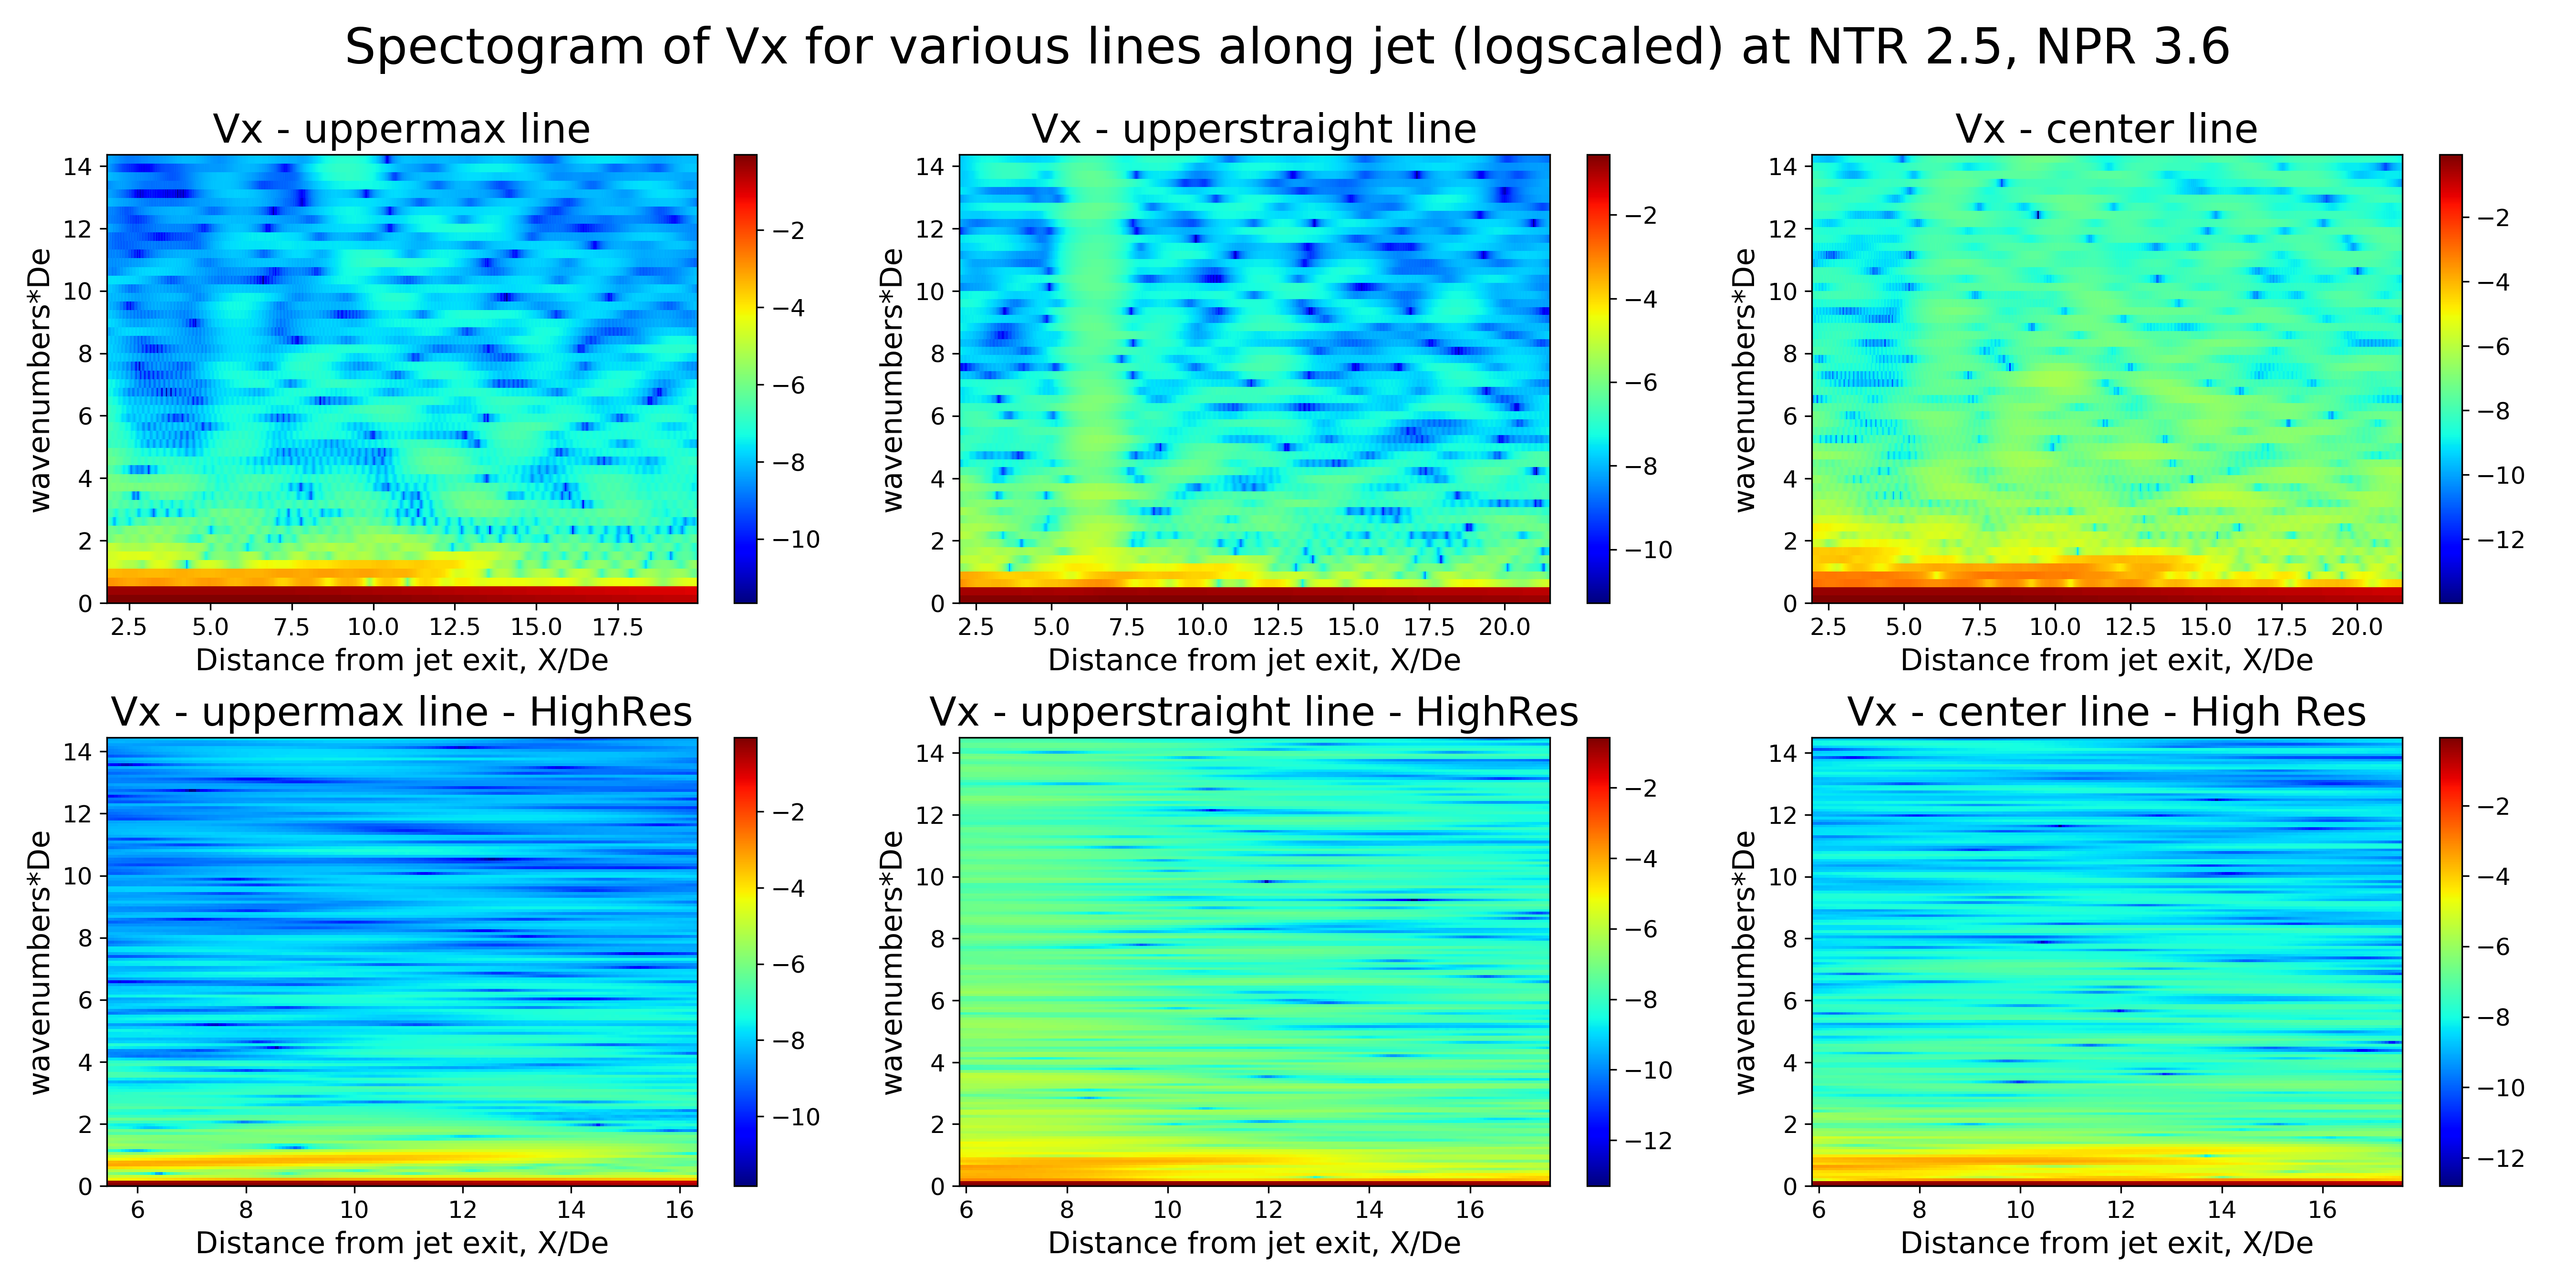
\includegraphics[width=3in]{images/Spectogram_Vx_NTR2p5_NPR3p6.png}
	\caption{NTR:2p5 NPR:3p6 }
	\label{fig:spectogramVx2p52p5}
\end{subfigure}%
\begin{subfigure}{0.5\textwidth}
	\centering
	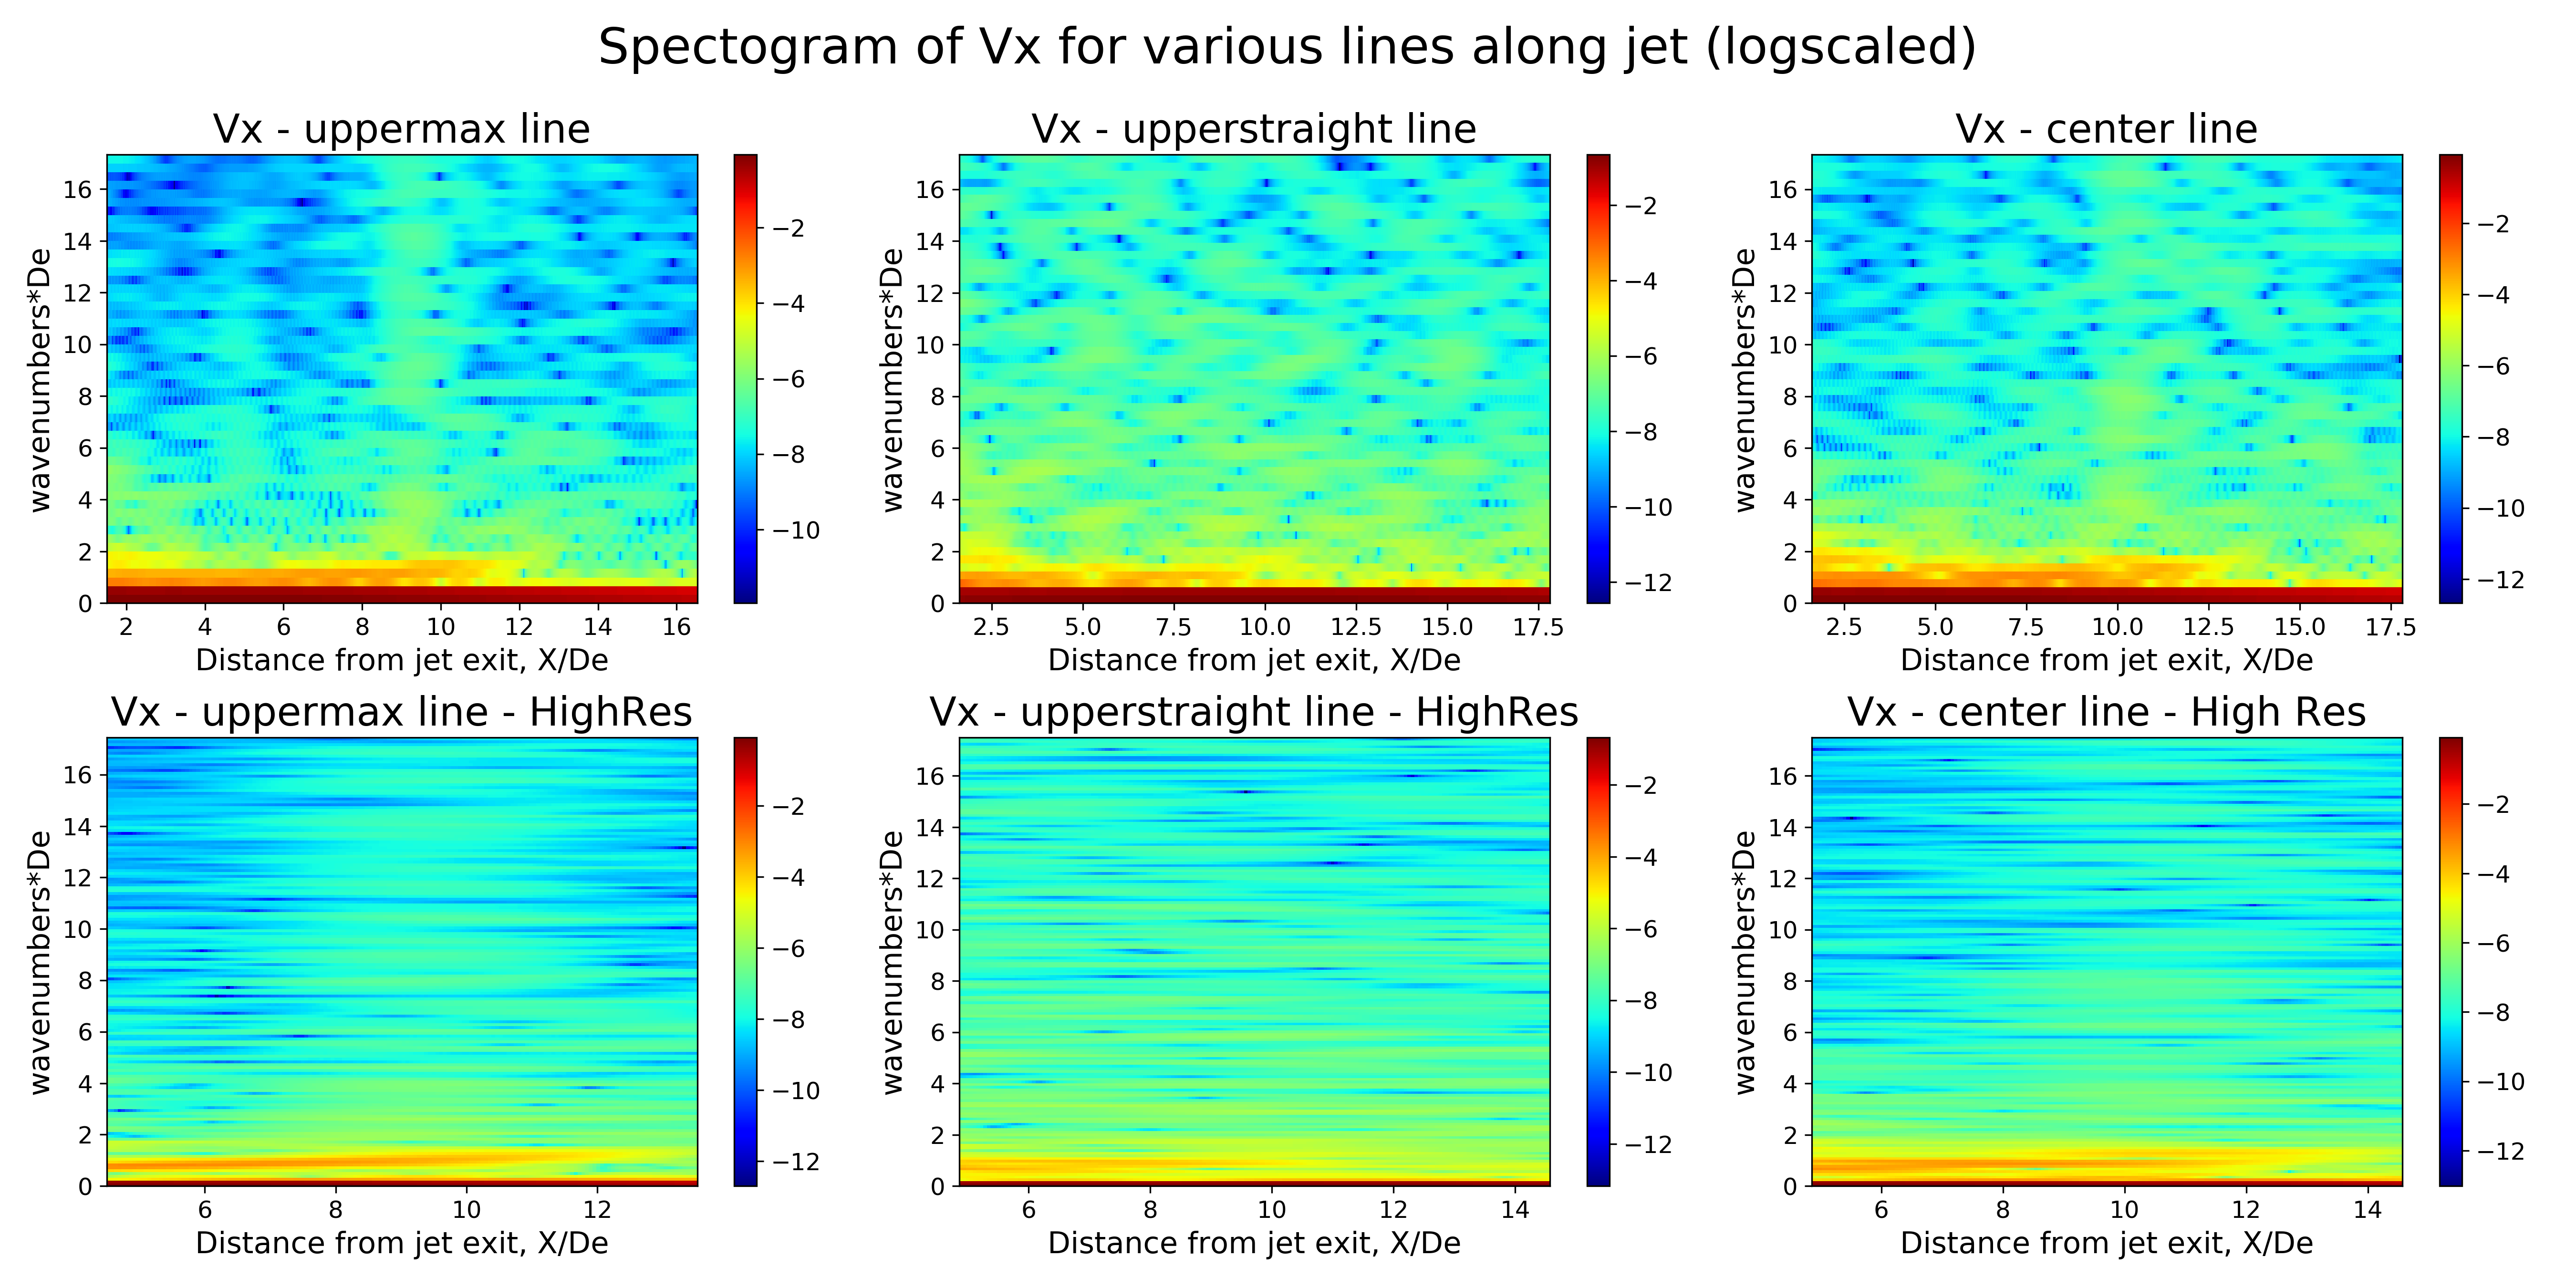
\includegraphics[width=3in]{images/Spectogram_Vx_NTR2p5_NPR4p0.png}
	\caption{NTR:2p5 NPR:4p0 }
	\label{fig:spectogramVx2p53p6}
\end{subfigure}
\caption{Spectogram plots for centreline $V_x$ without chevrons }
\label{fig:spectogramVx}
\end{figure} 

\begin{figure}[H]
\begin{subfigure}{0.5\textwidth}
	\centering
	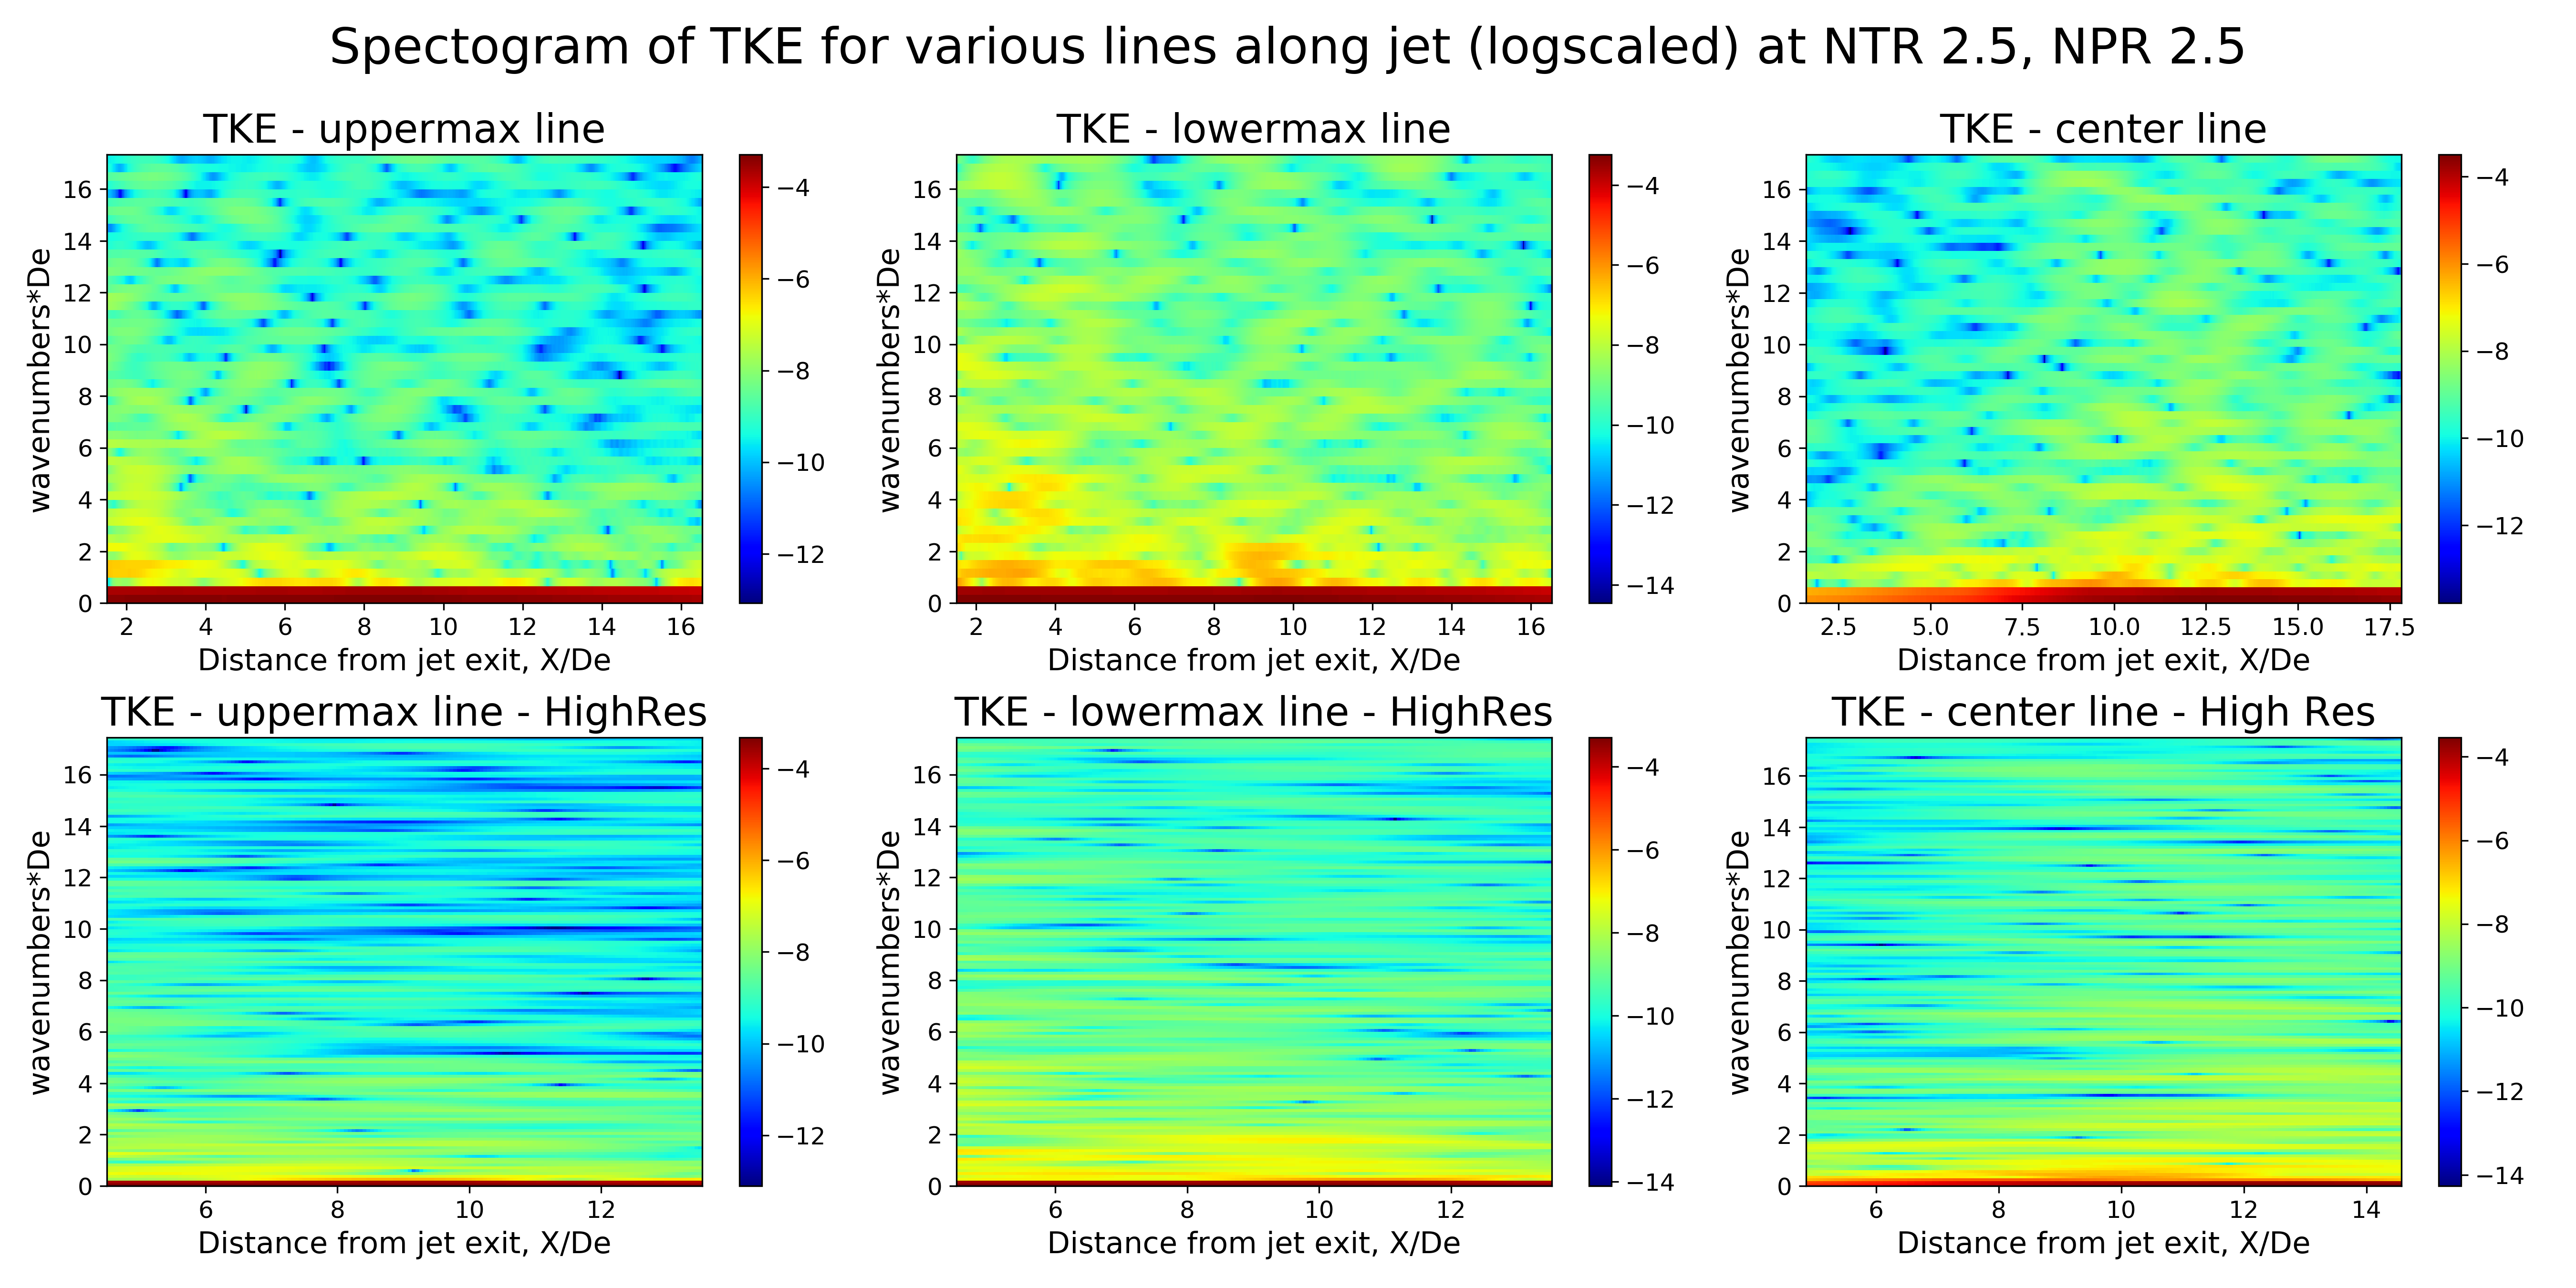
\includegraphics[width=3in]{images/Spectogram_TKE_NTR2p5_NPR2p5.png}
	\caption{NTR:2p5 NPR:2p5 }
	\label{fig:spectogramTKE2p52p5}
\end{subfigure}%
\begin{subfigure}{0.5\textwidth}
	\centering
	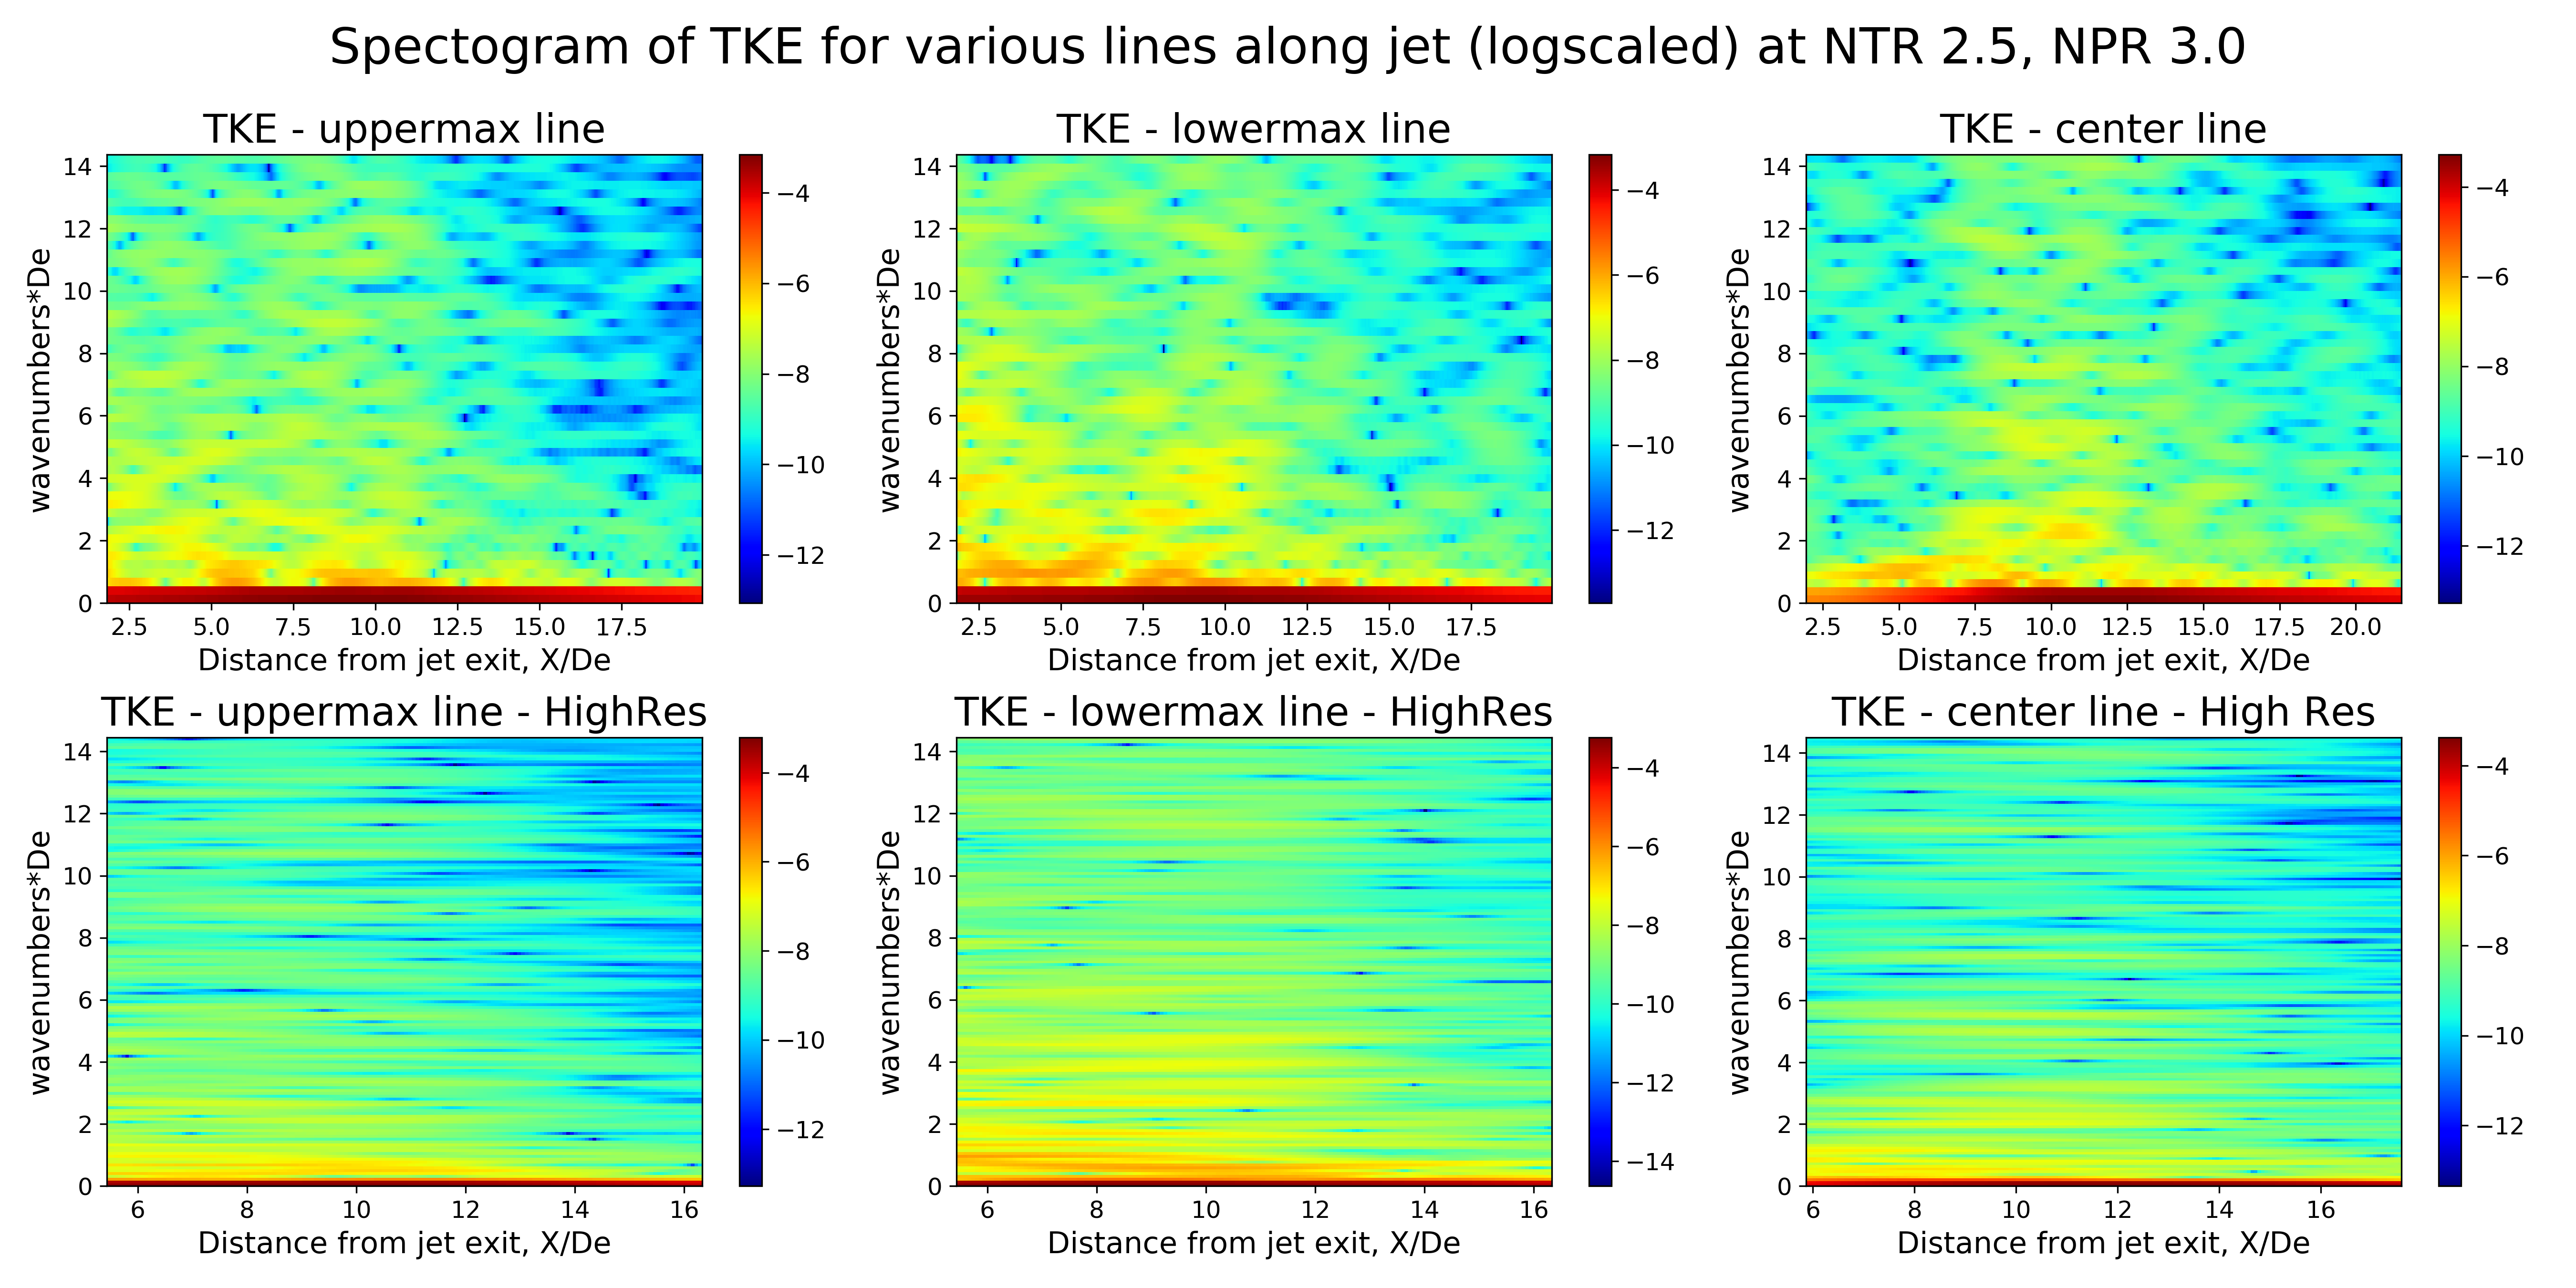
\includegraphics[width=3in]{images/Spectogram_TKE_NTR2p5_NPR3p0.png}
	\caption{NTR:2p5 NPR:3p6 }
	\label{fig:spectogramTKE2p53p0}
\end{subfigure}\\
\begin{subfigure}{0.5\textwidth}
	\centering
	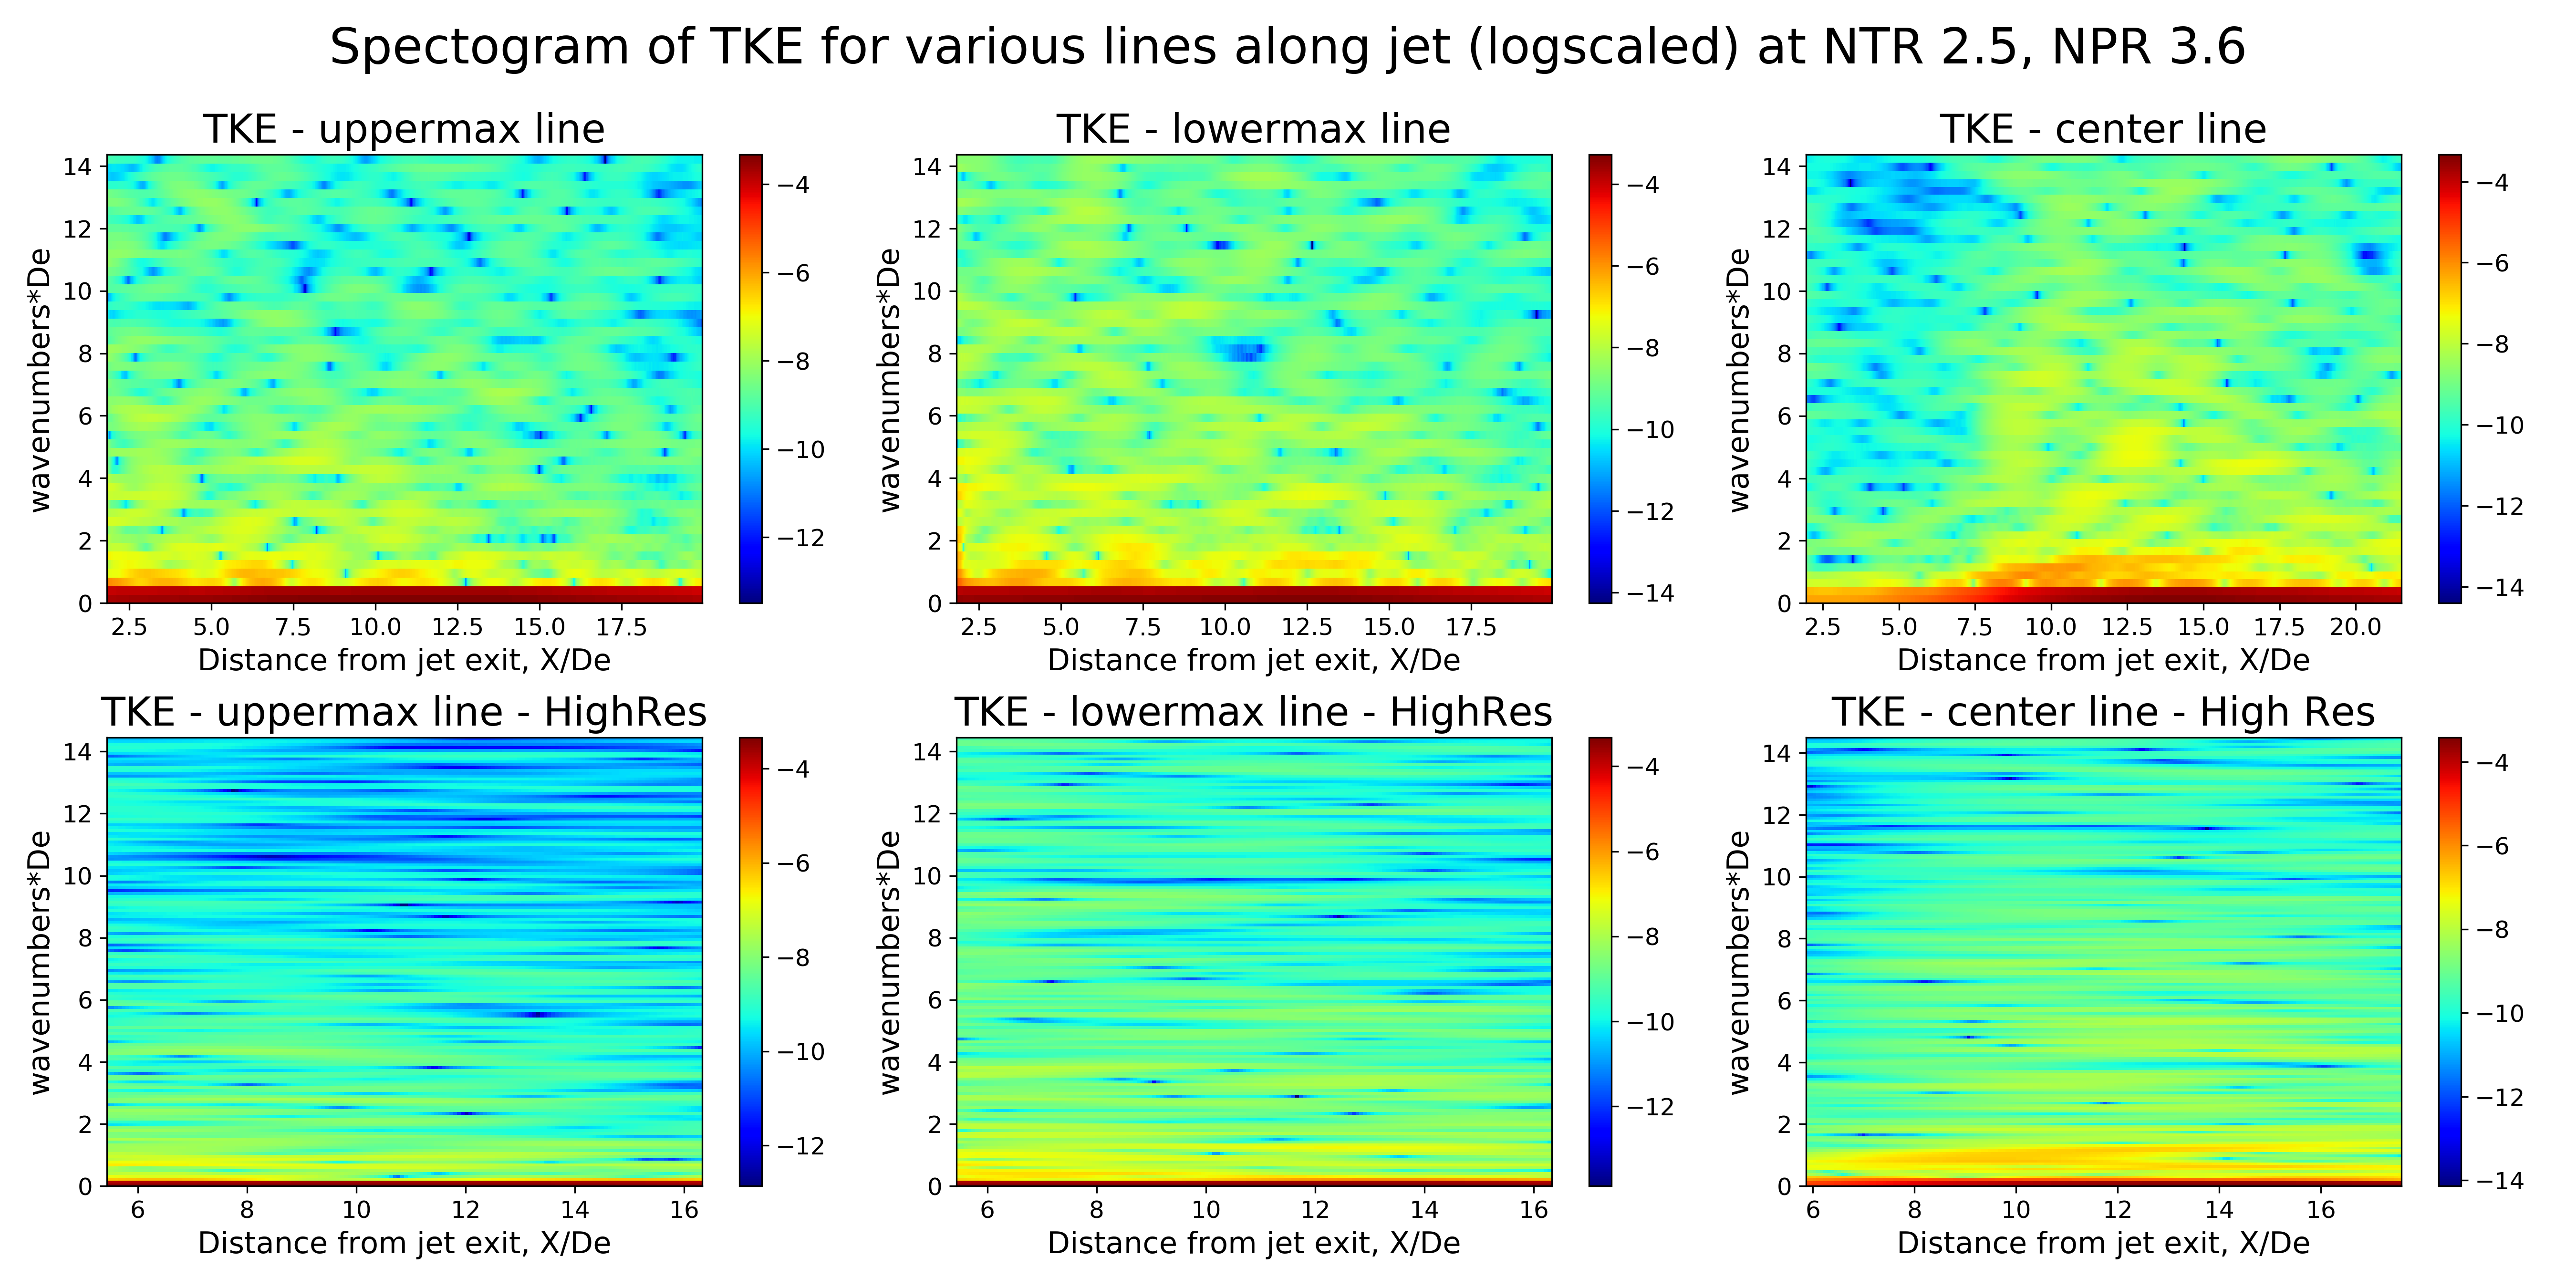
\includegraphics[width=3in]{images/Spectogram_TKE_NTR2p5_NPR3p6.png}
	\caption{NTR:2p5 NPR:2p5 }
	\label{fig:spectogramTKE2p53p6}
\end{subfigure}%
\begin{subfigure}{0.5\textwidth}
	\centering
	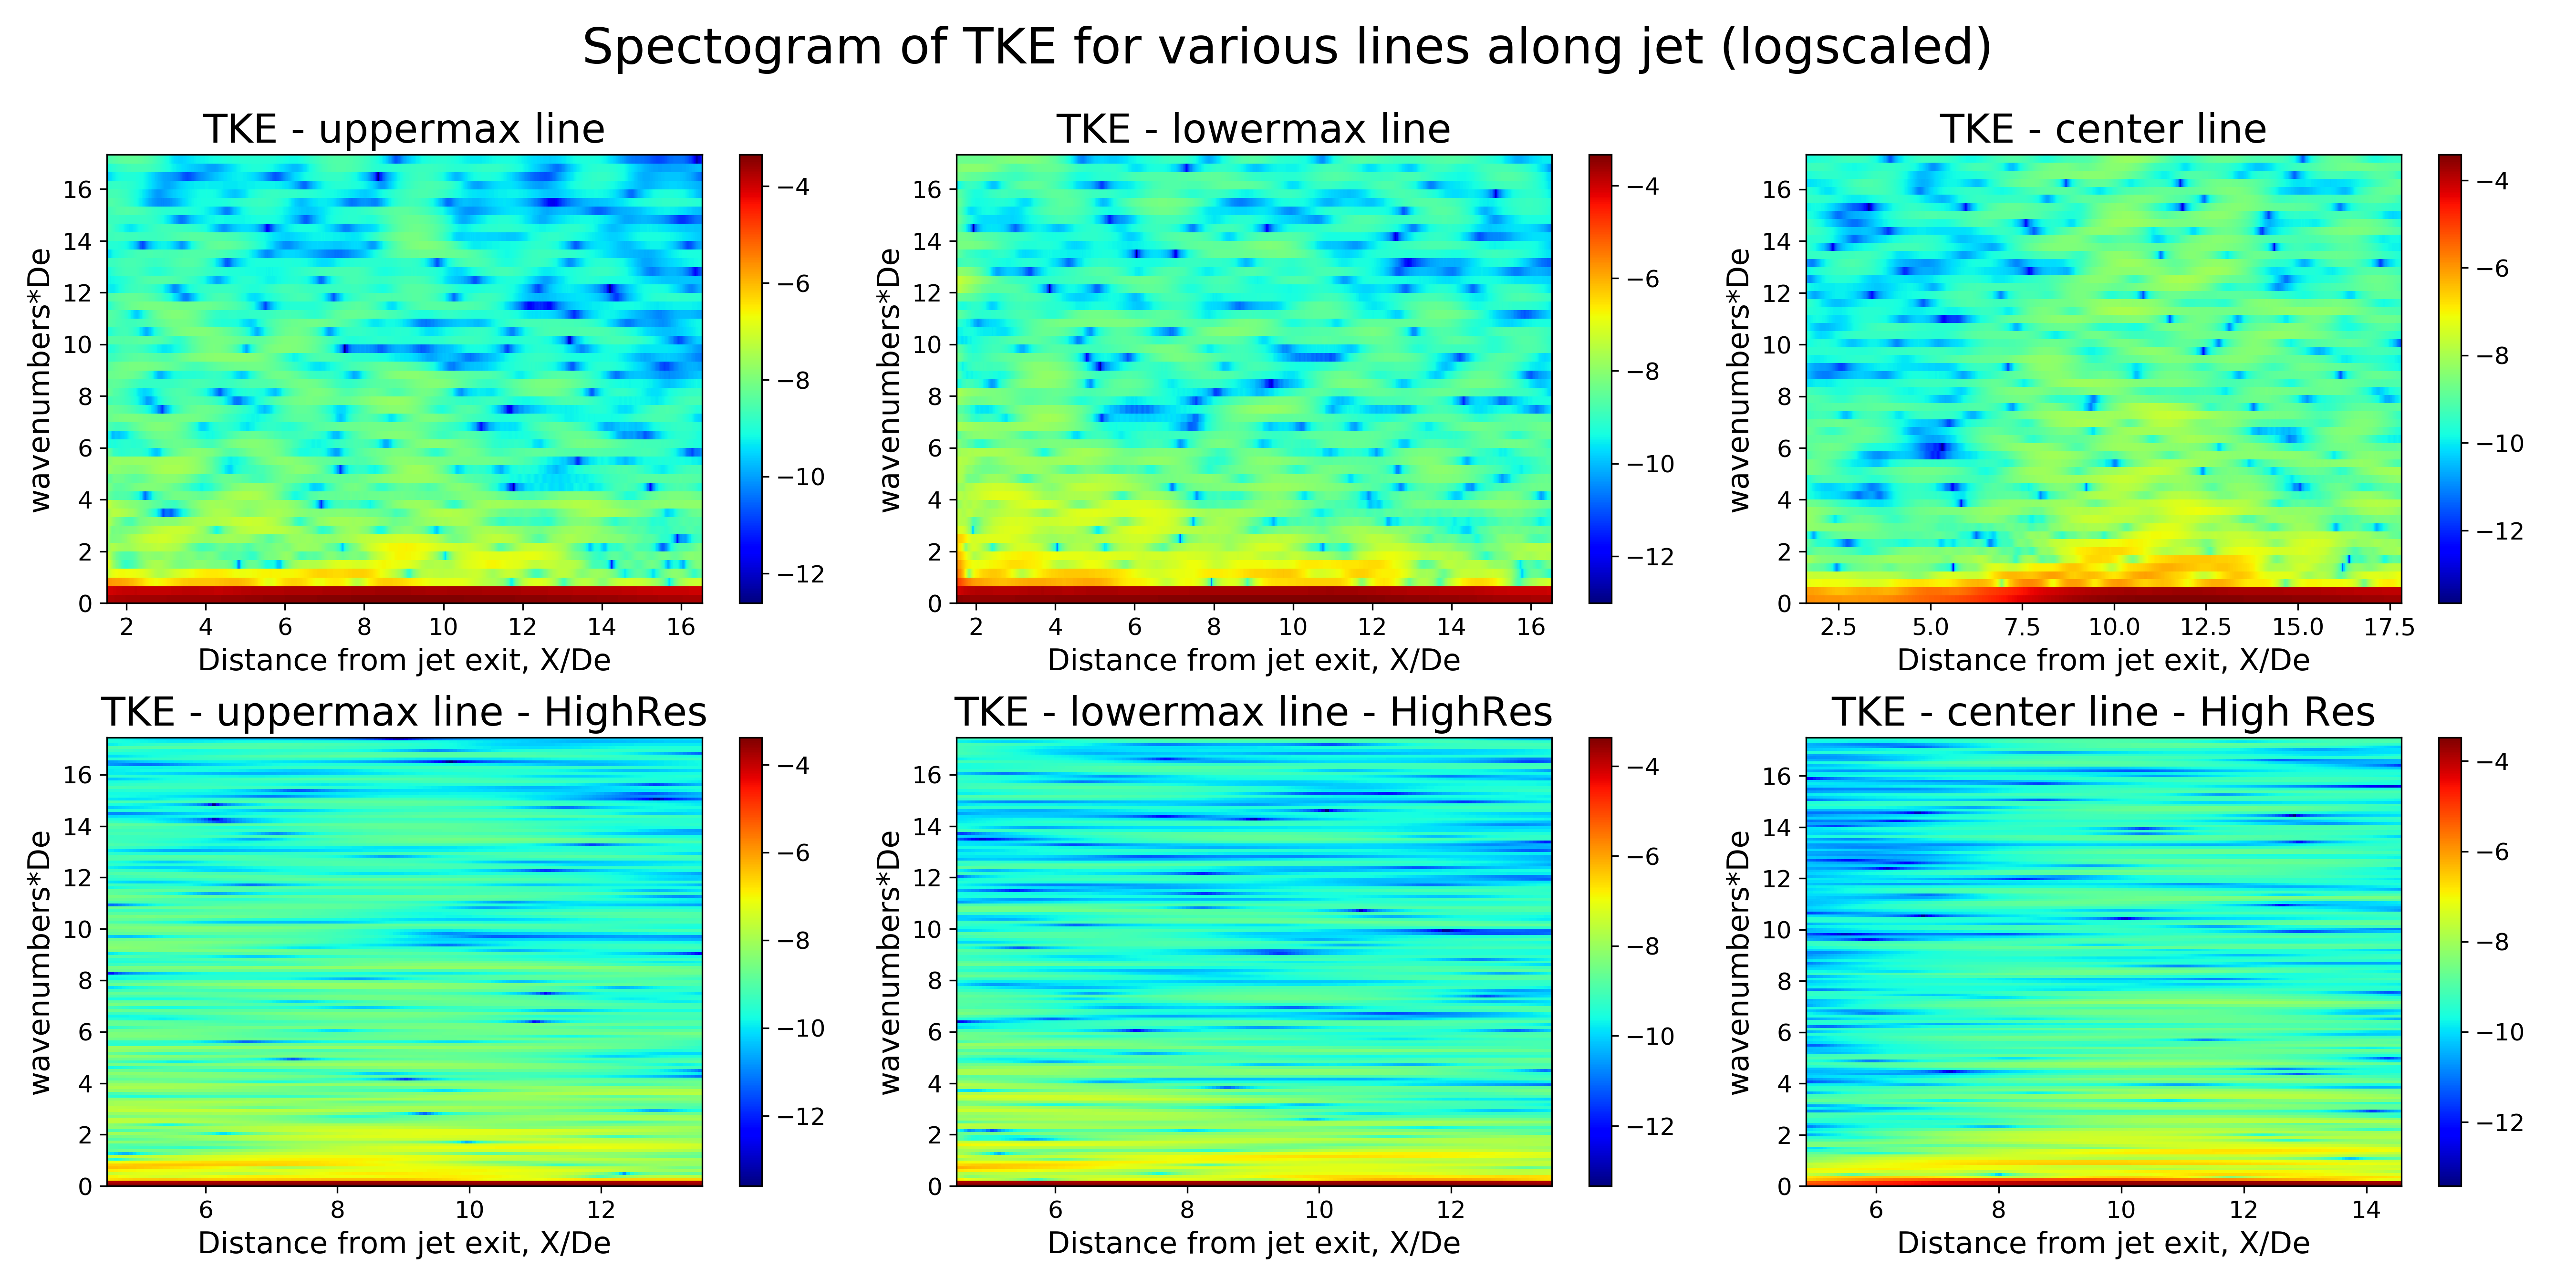
\includegraphics[width=3in]{images/Spectogram_TKE_NTR2p5_NPR4p0.png}
	\caption{NTR:2p5 NPR:3p6 }
	\label{fig:spectogramTKE2p54p0}
\end{subfigure}
\caption{Spectogram plots for centreline TKE without chevrons }
\label{fig:spectogramTKE}
\end{figure} 

Spectogram of TKE(fig \ref{fig:spectogramTKE}) can also be similarly used to estimate the end of potential core. This wavelength spectrum could also be helpful for modelling acoustic sources along the jet. \\ 

\section{Effect of Chevron}  

Only three cases, all perfectly expanded flows for different temperatures, have been studied with chevrons. Fig shows that the temperature doesn't affect the wavelength value but clearly reducing the intensity of pattern as seen before without chevrons. Also, we can notice that now the wavelength is about 25-30\% less than the values obtained without chevrons. This shows that chevrons are decreasing the length of shock cells, perhaps by increasing mixing between layers. This is as expected from the discussion in Heeb et.al.\cite{heeb} which is the reason BBSN tends to shift towards higher frequency. From fig \ref{fig:lineplotsTKE}, Point of merging of centreline plots  with lines at lips is closer to exit at each temperature implying the decrease in potential core length. Also, increase in temperature decreases potential core length for both with and without chevrons. 

\begin{figure}[H]
\begin{subfigure}{.5\textwidth}
	\centering
	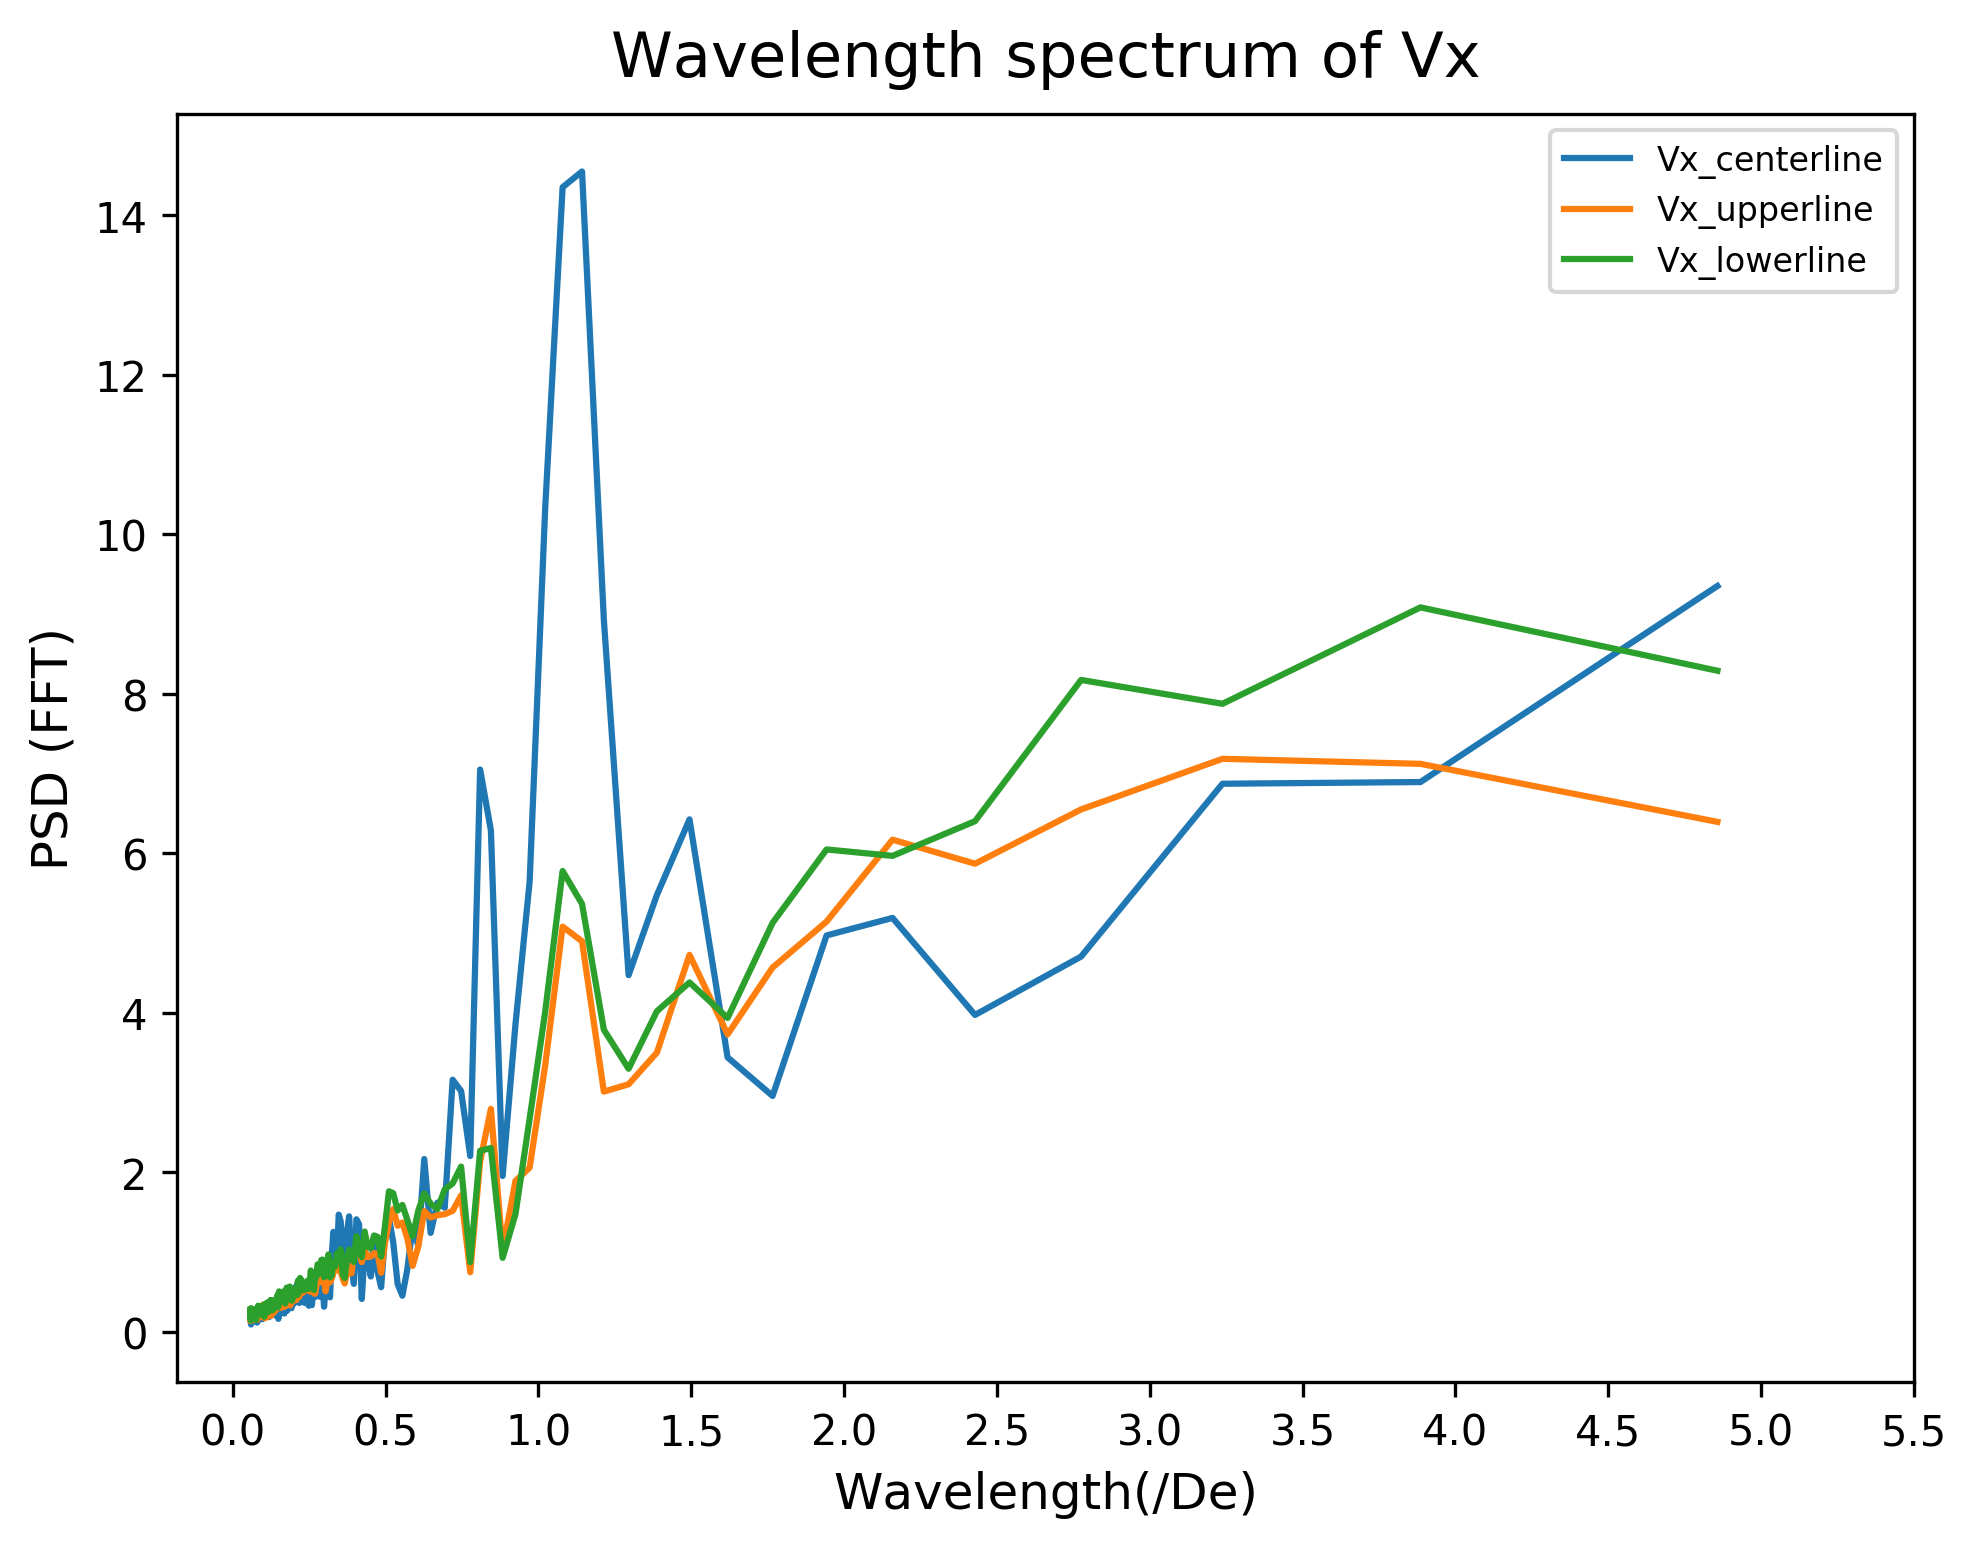
\includegraphics[width=2.5in]{images/Fft_Vx_NTR1p0_NPR3p6c.png}
	\caption{NTR:1p0 NPR:3p6 with chevrons }
	\label{fig:fftplotsc1p03p6}
\end{subfigure}%
\begin{subfigure}{.5\textwidth}
	\centering
	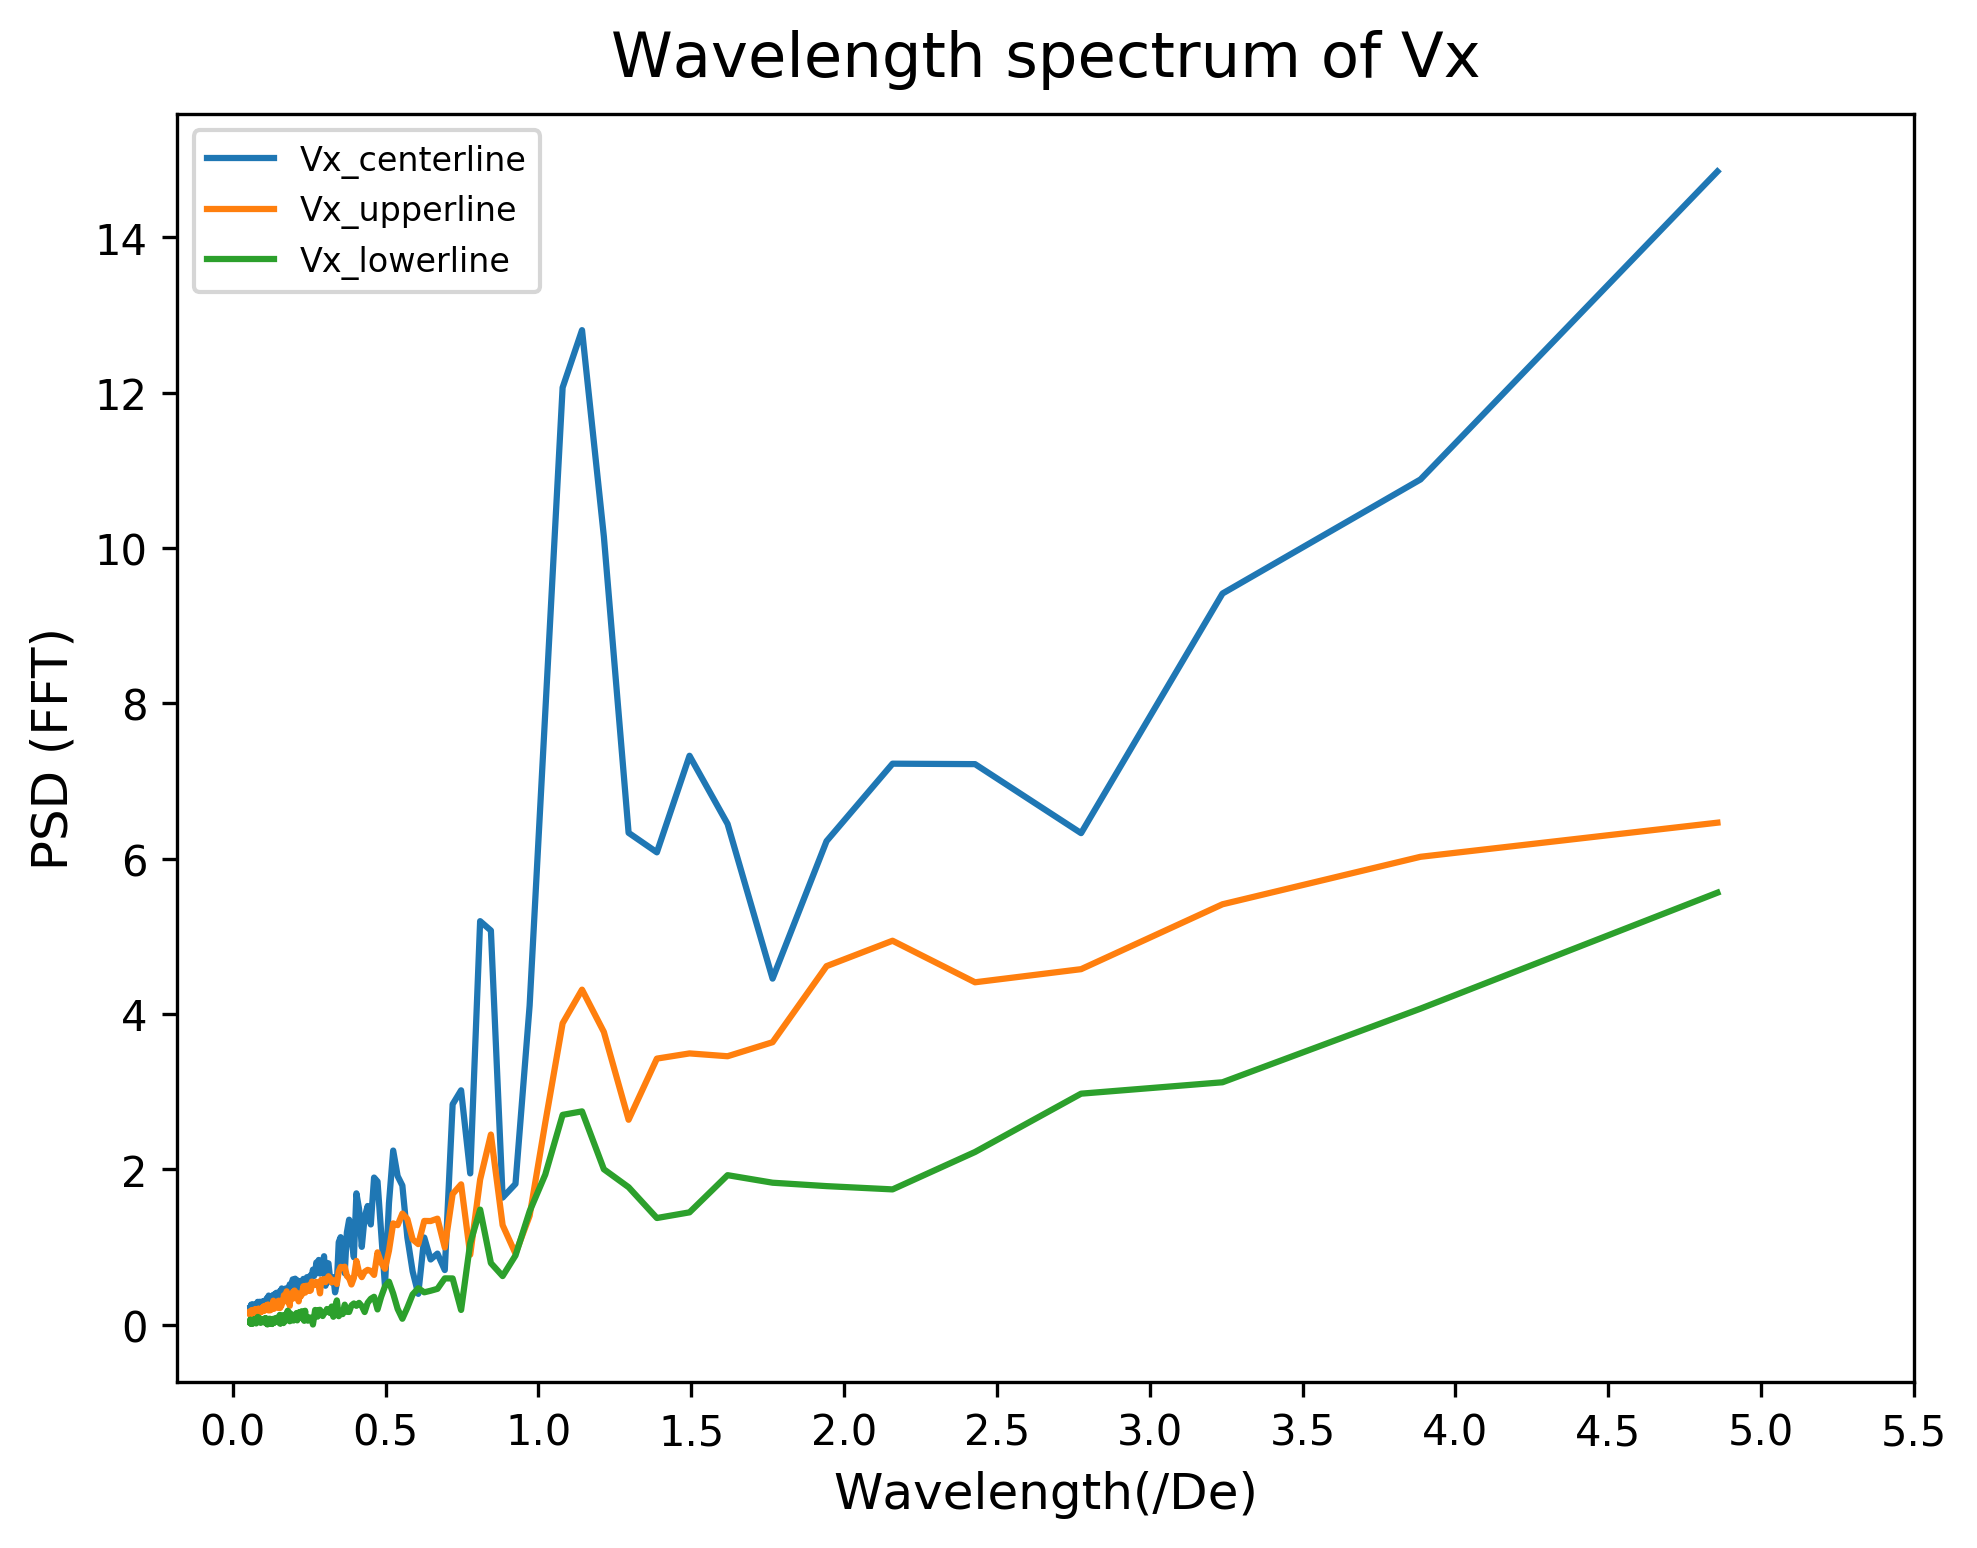
\includegraphics[width=2.5in]{images/Fft_Vx_NTR2p0_NPR3p6c.png}
	\caption{NTR:2p0 NPR:3p6 with chevrons}
	\label{fig:fftplotsc2p03p6}
\end{subfigure}
\begin{subfigure}{1.0\textwidth}
	\centering
	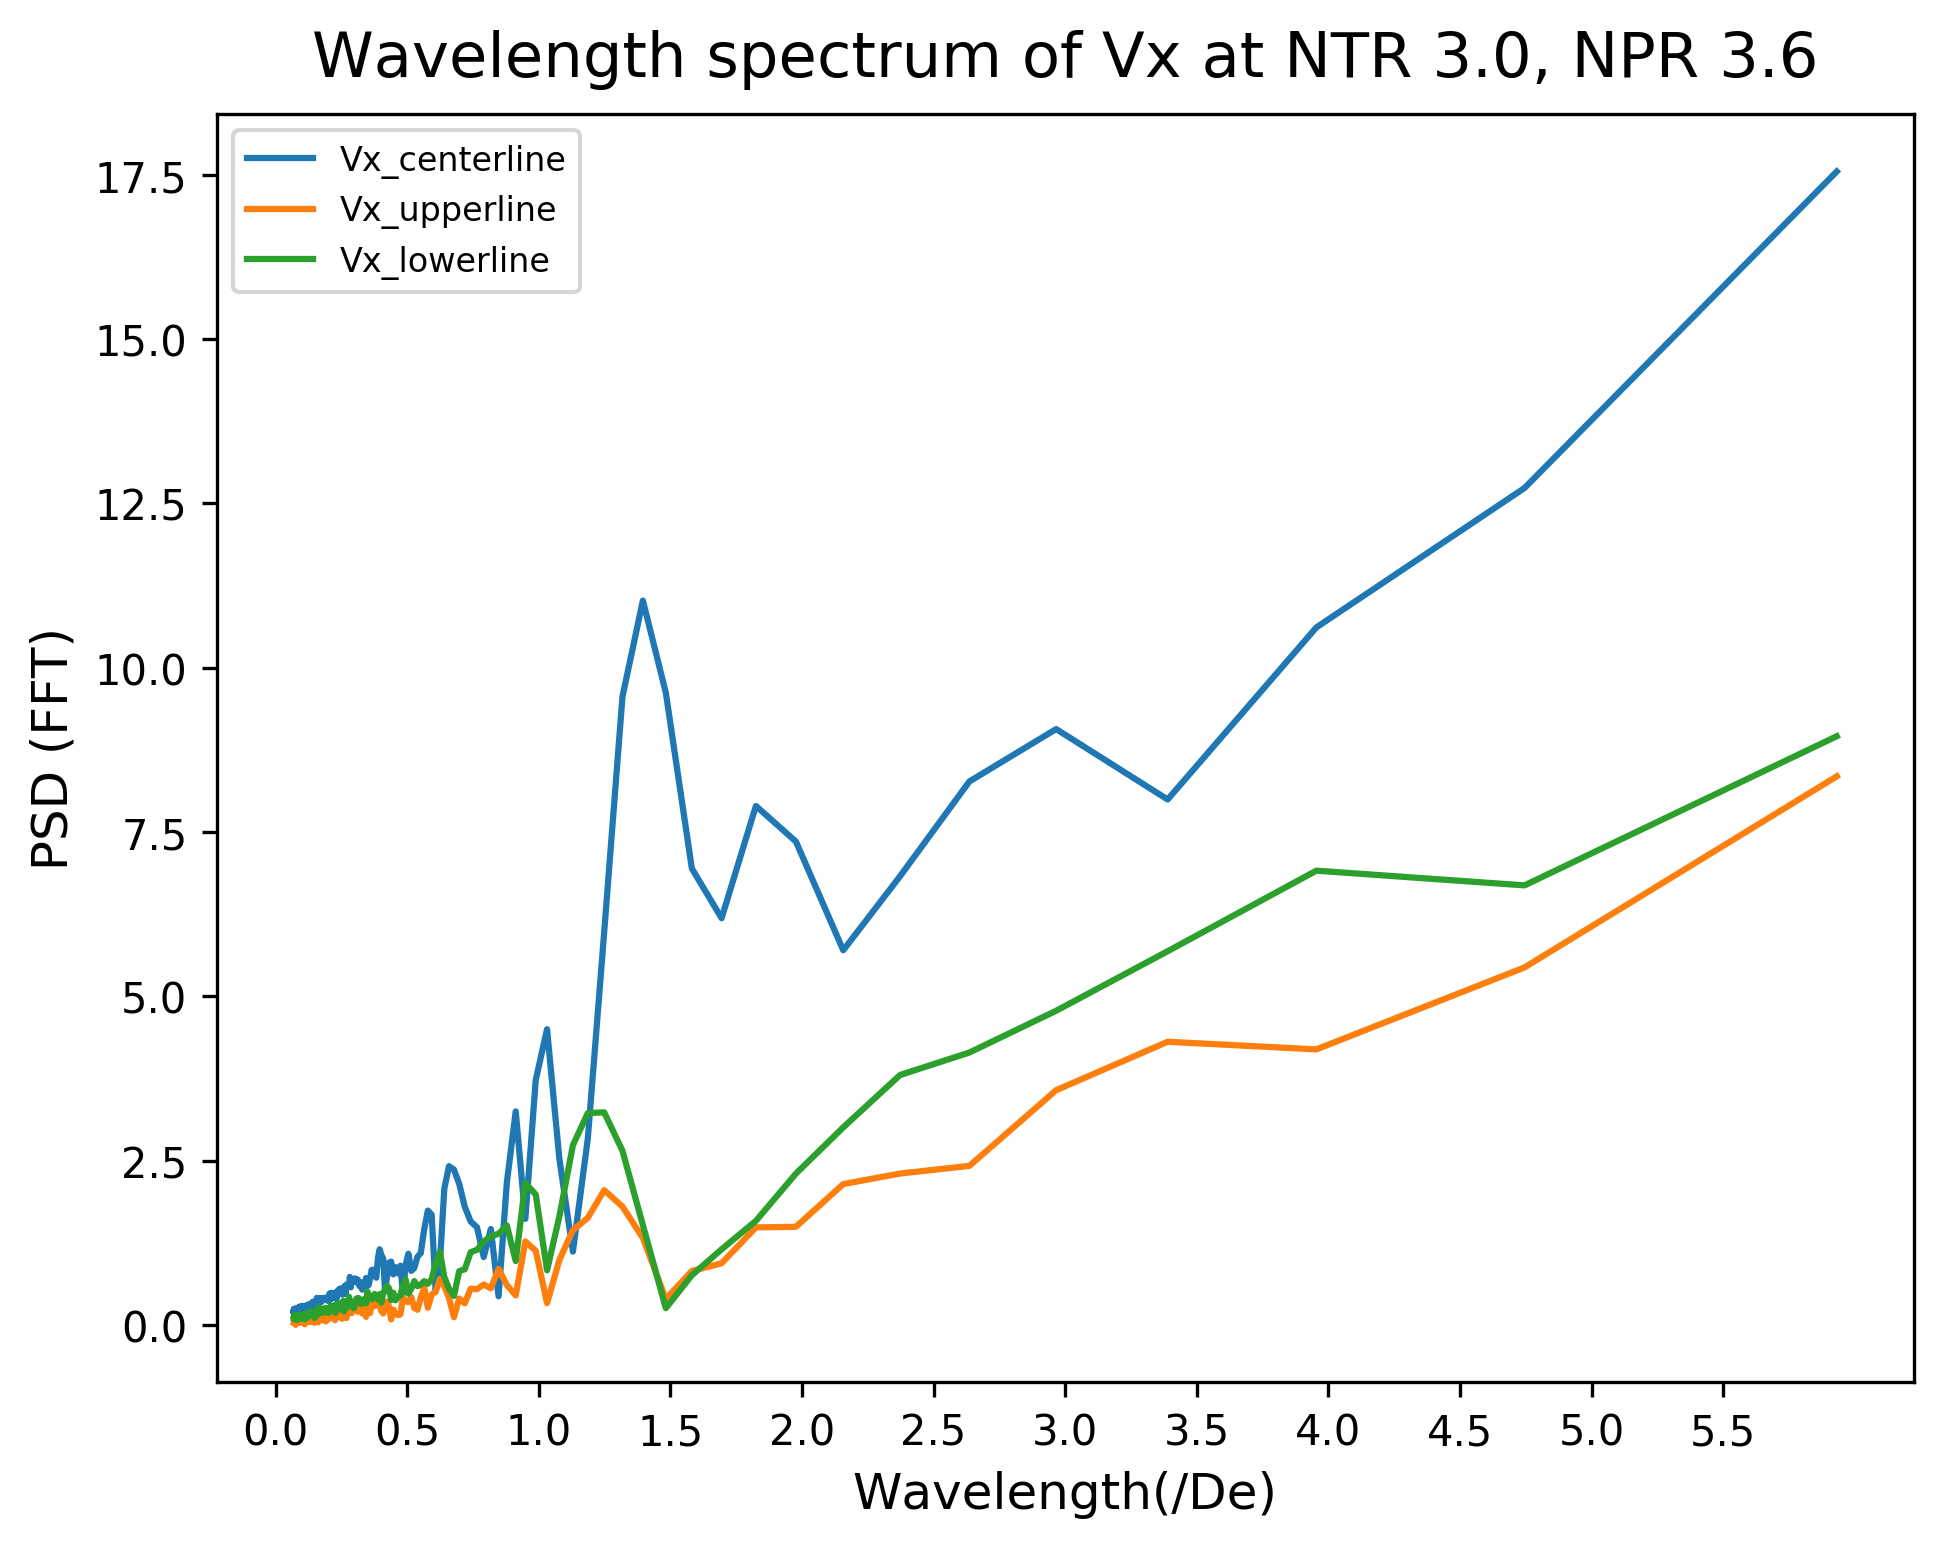
\includegraphics[width=2.5in]{images/Fft_Vx_NTR3p0_NPR3p6c.png}
	\caption{NTR:3p0 NPR:3p6 with chevrons}
	\label{fig:fftplotsc3p03p6}
\end{subfigure}%
\caption{wavelength spectrum using FFT for centreline $V_x$ with  chevrons }
\label{fig:fftplotsc}
\end{figure}

Another interesting observation (fig \ref{fig:lineplotsTKE}) is considerable increase in TKE fluctuations on centreline because of chevrons although TKE at lips of jet is not affected much. Reduction in screech tone with chevrons, widely observed, can still be explained with possible increase in difference between frequencies of acoustic waves exciting thin shear layer and flow structure-shock interaction. But reduction in BBSN amplitude as reported in Heeb et.al.\cite{heeb} is counterintuitive with what is being observed here and shows that influence of chevrons on BBSN needs more attention. 

\begin{figure}[H]
\begin{subfigure}{.5\textwidth}
	\centering
	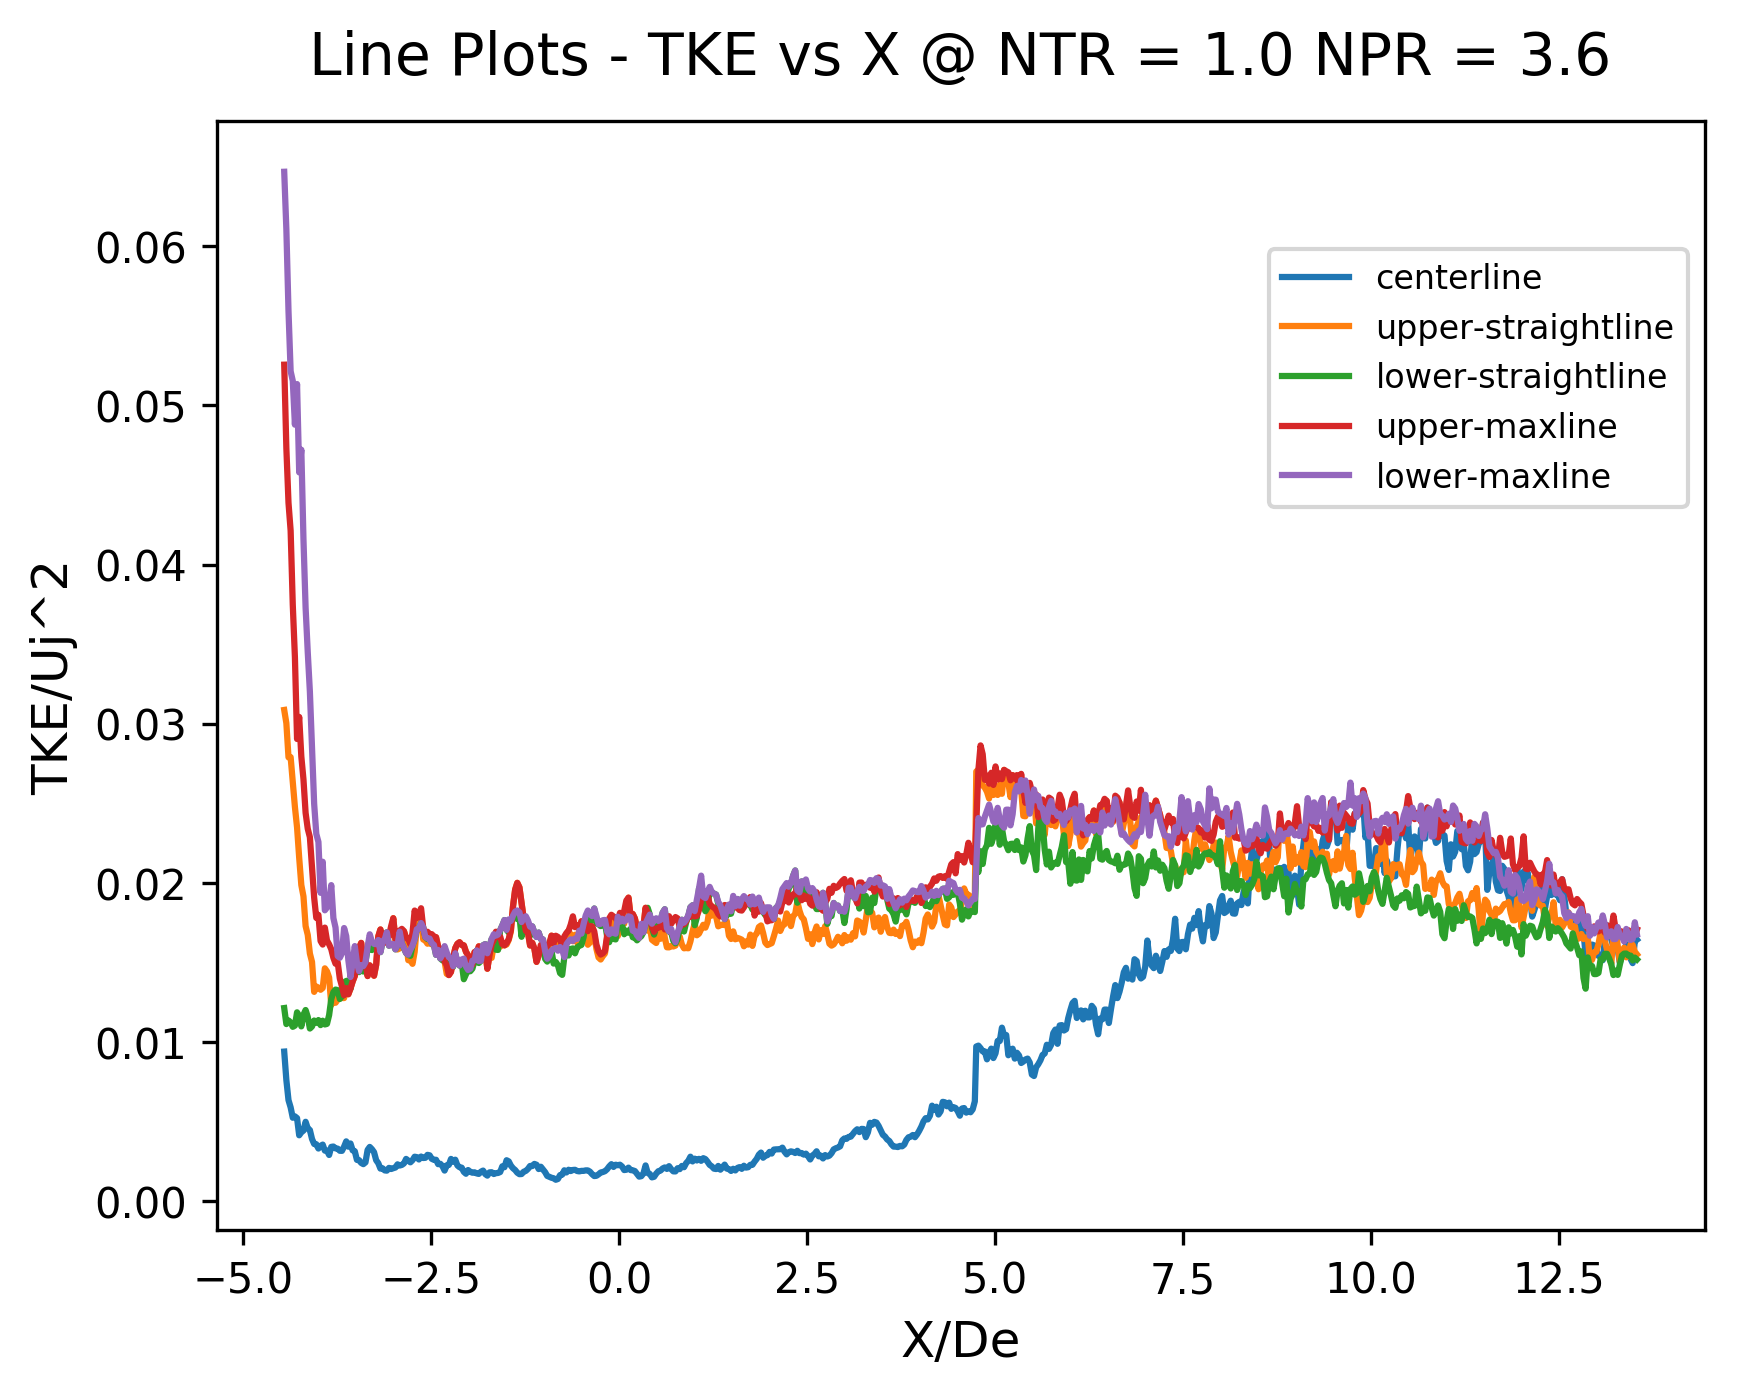
\includegraphics[width=2.5in]{images/LinePlots_TKE_NTR1p0_NPR3p6.png}
	\caption{NTR:1p0 NPR:3p6 without chevrons }
	\label{fig:lineplotsTKE1p03p6}
\end{subfigure}%
\begin{subfigure}{.5\textwidth}
	\centering
	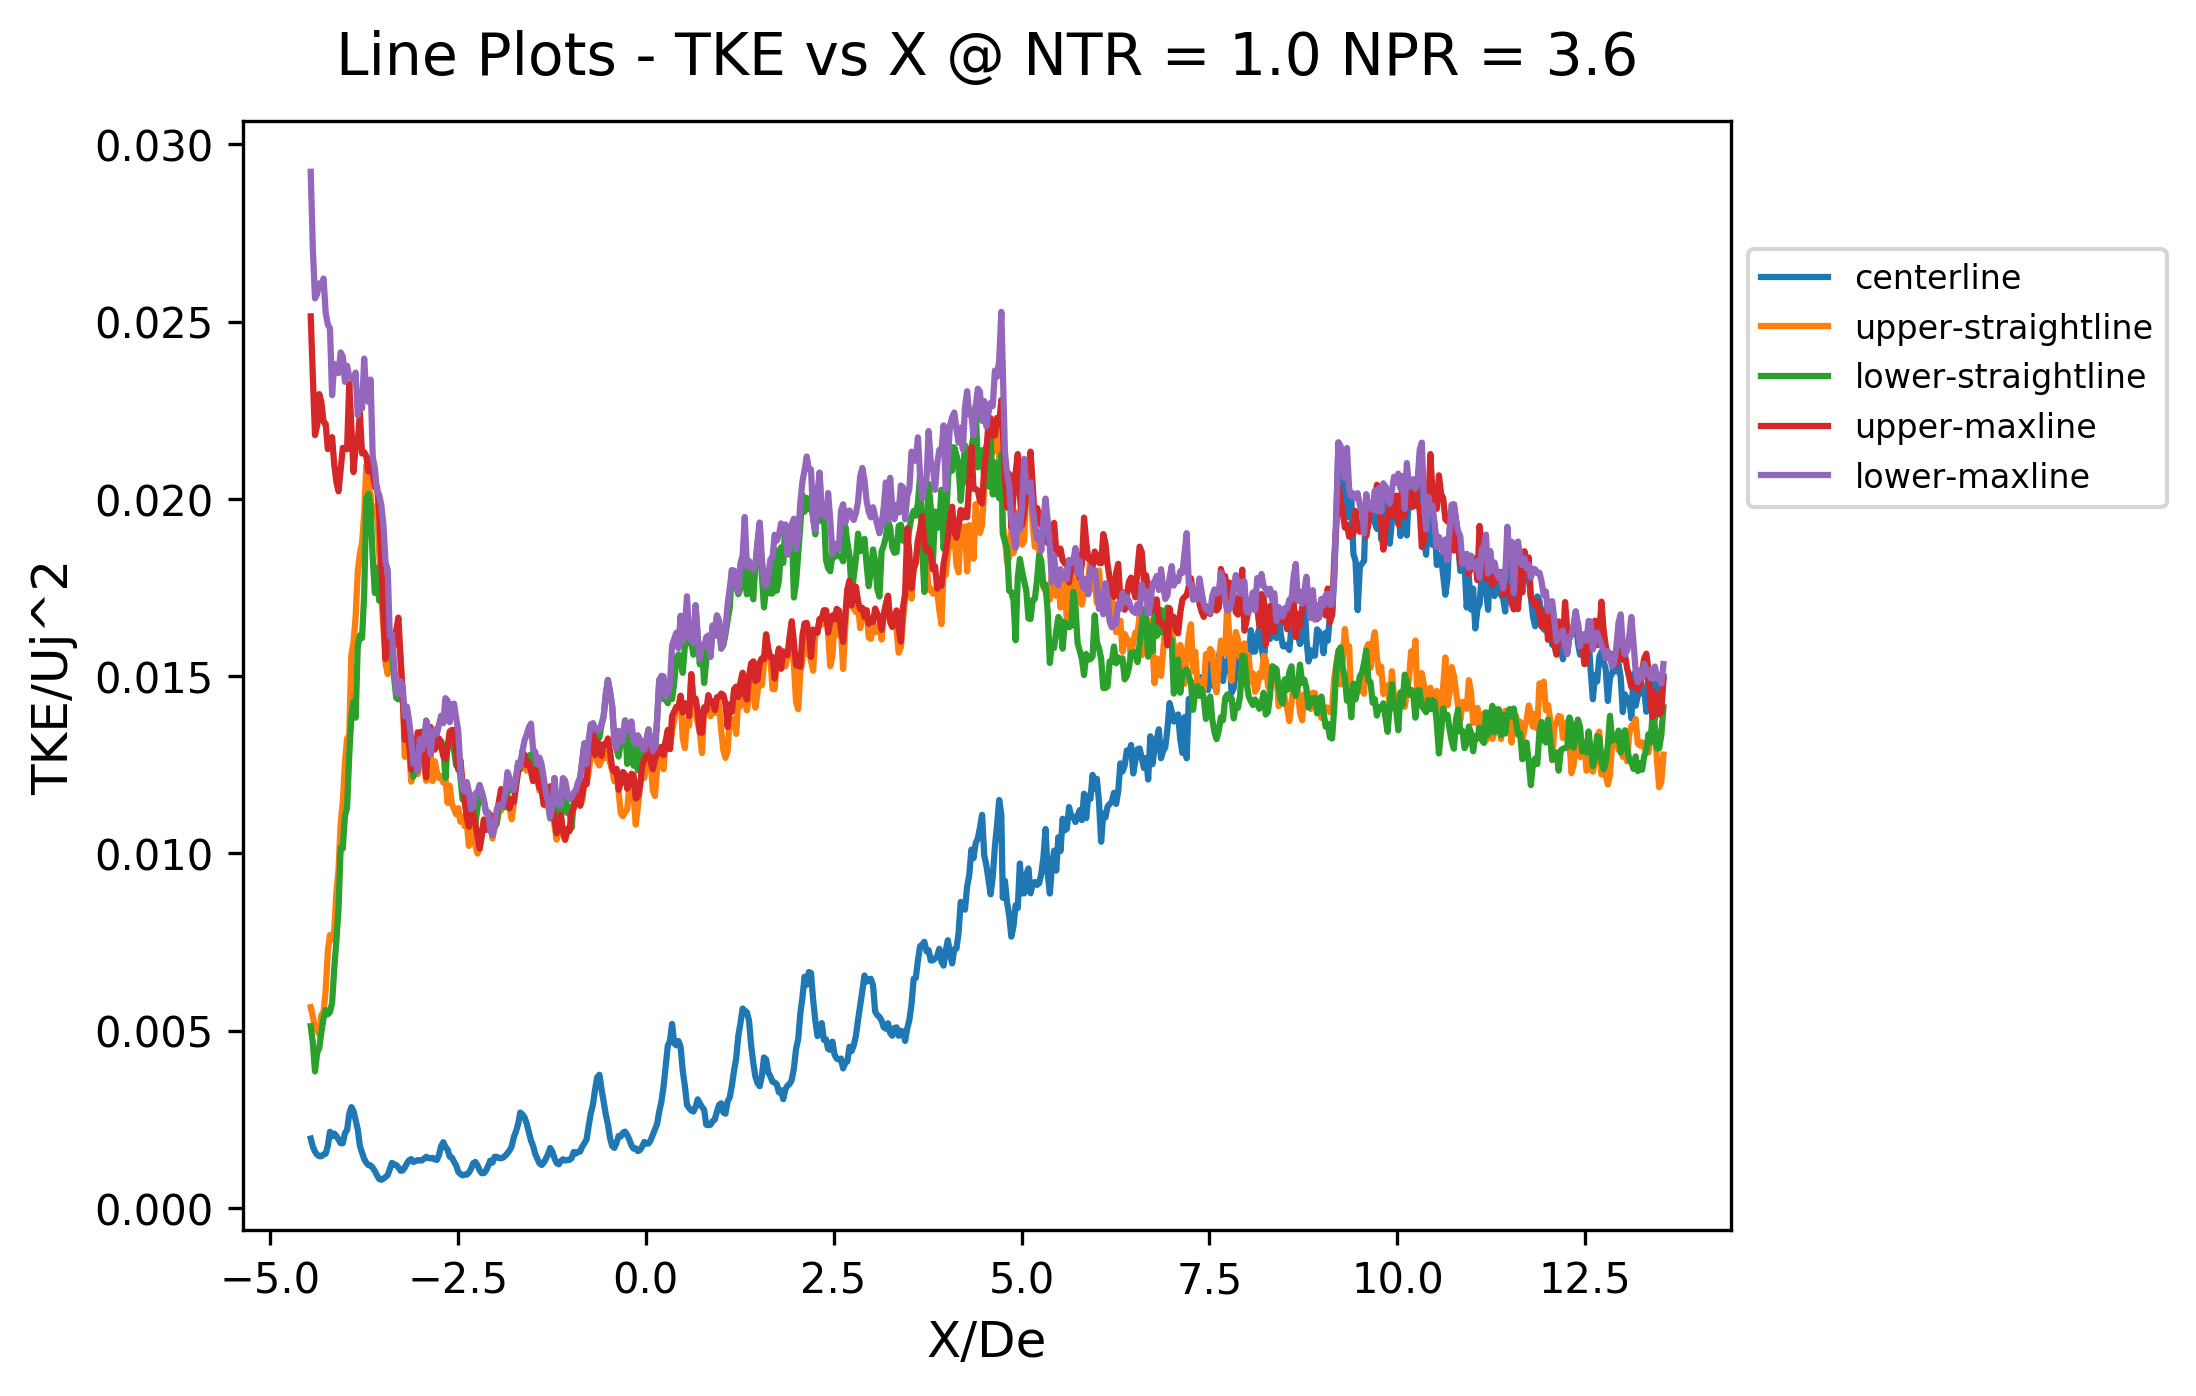
\includegraphics[width=3.25in]{images/LinePlots_TKE_NTR1p0_NPR3p6c.png}
	\caption{NTR:1p0 NPR:3p6 with chevrons}
	\label{fig:lineplotsTKE1p03p6c}
\end{subfigure}
\begin{subfigure}{.5\textwidth}
	\centering
	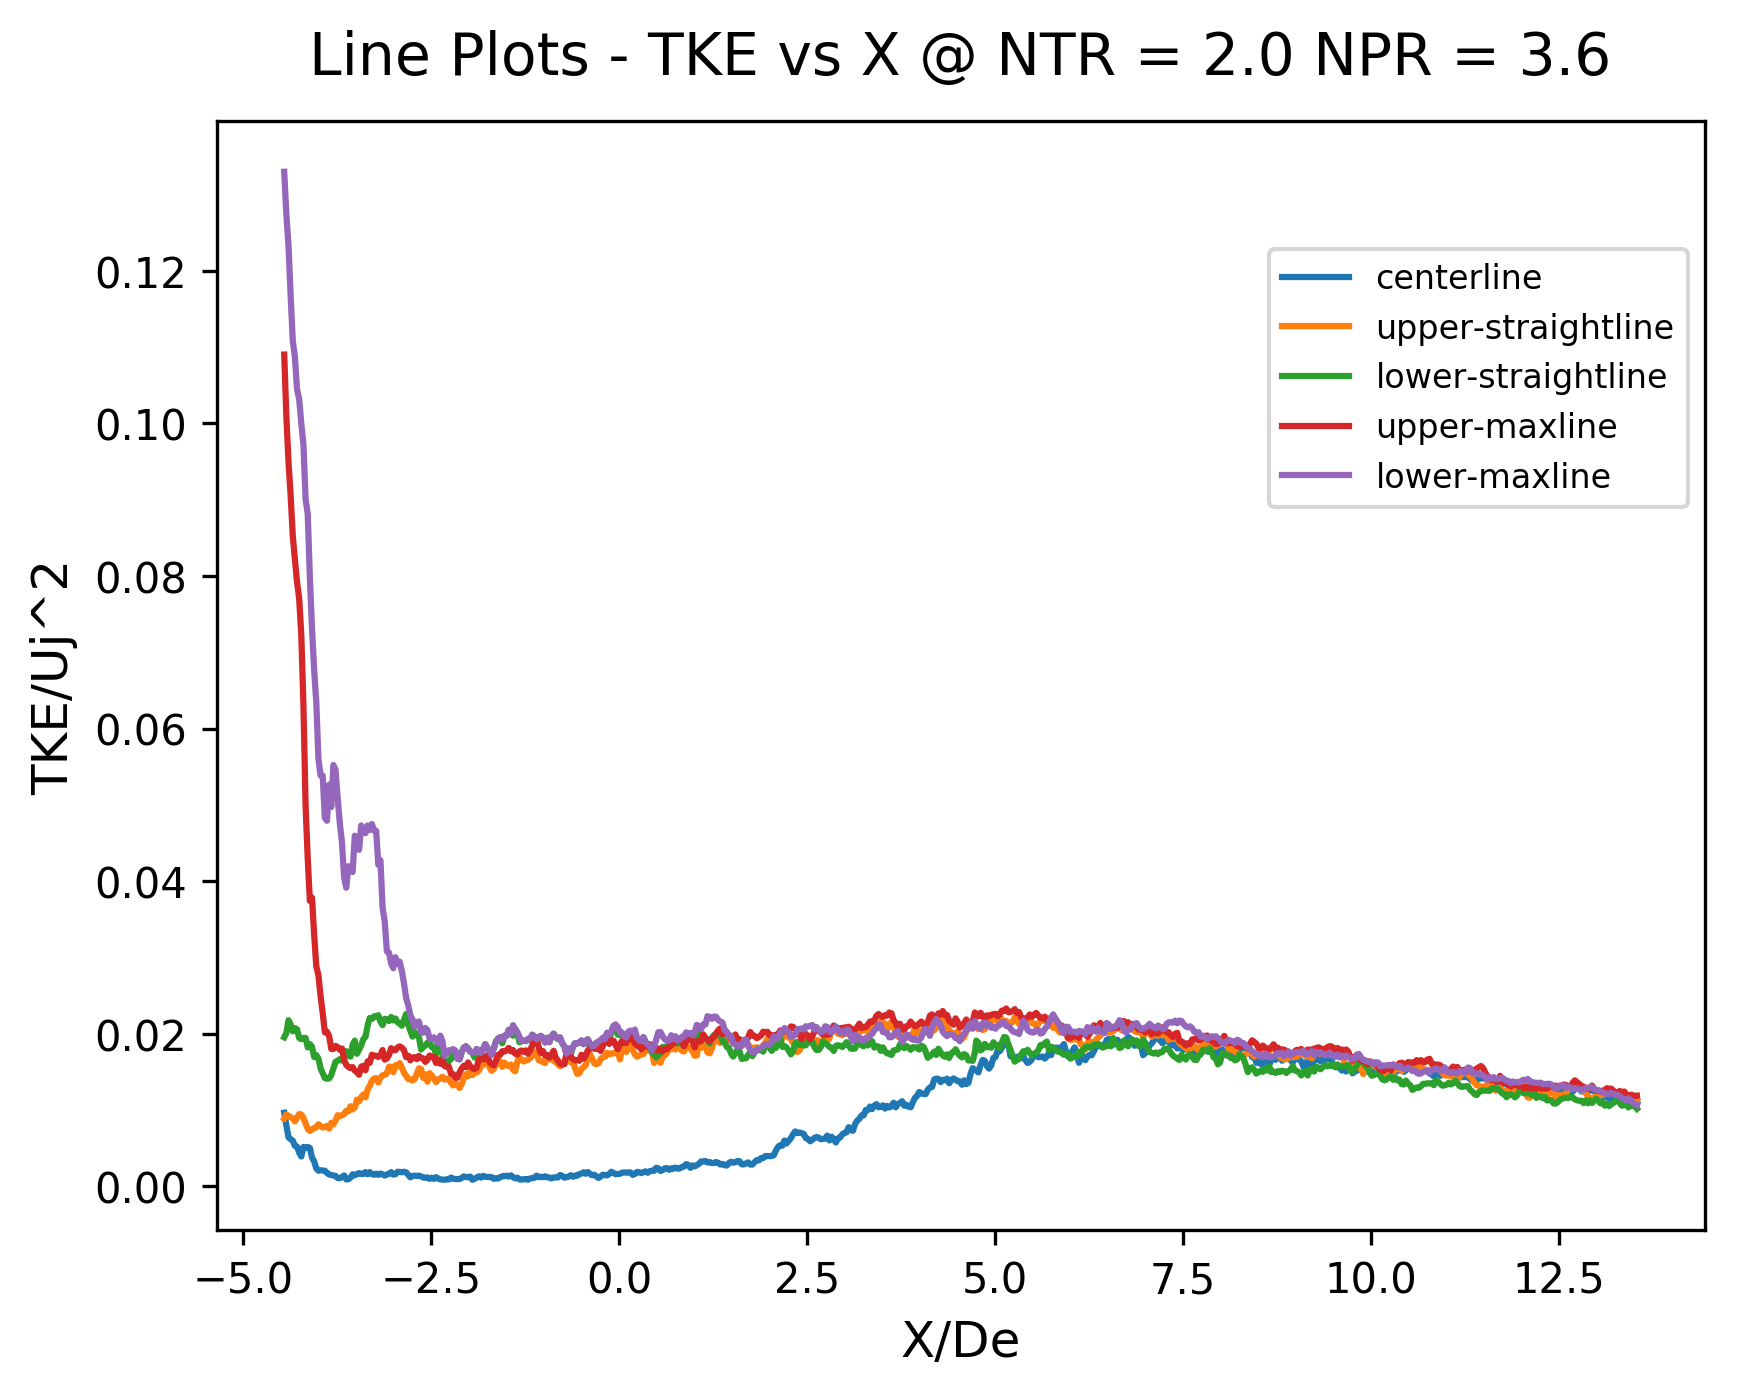
\includegraphics[width=2.5in]{images/LinePlots_TKE_NTR2p0_NPR3p6.png}
	\caption{NTR:2p0 NPR:3p6 without chevrons}
	\label{fig:lineplotsTKE2p03p6}
\end{subfigure}%
\begin{subfigure}{.5\textwidth}
	\centering
	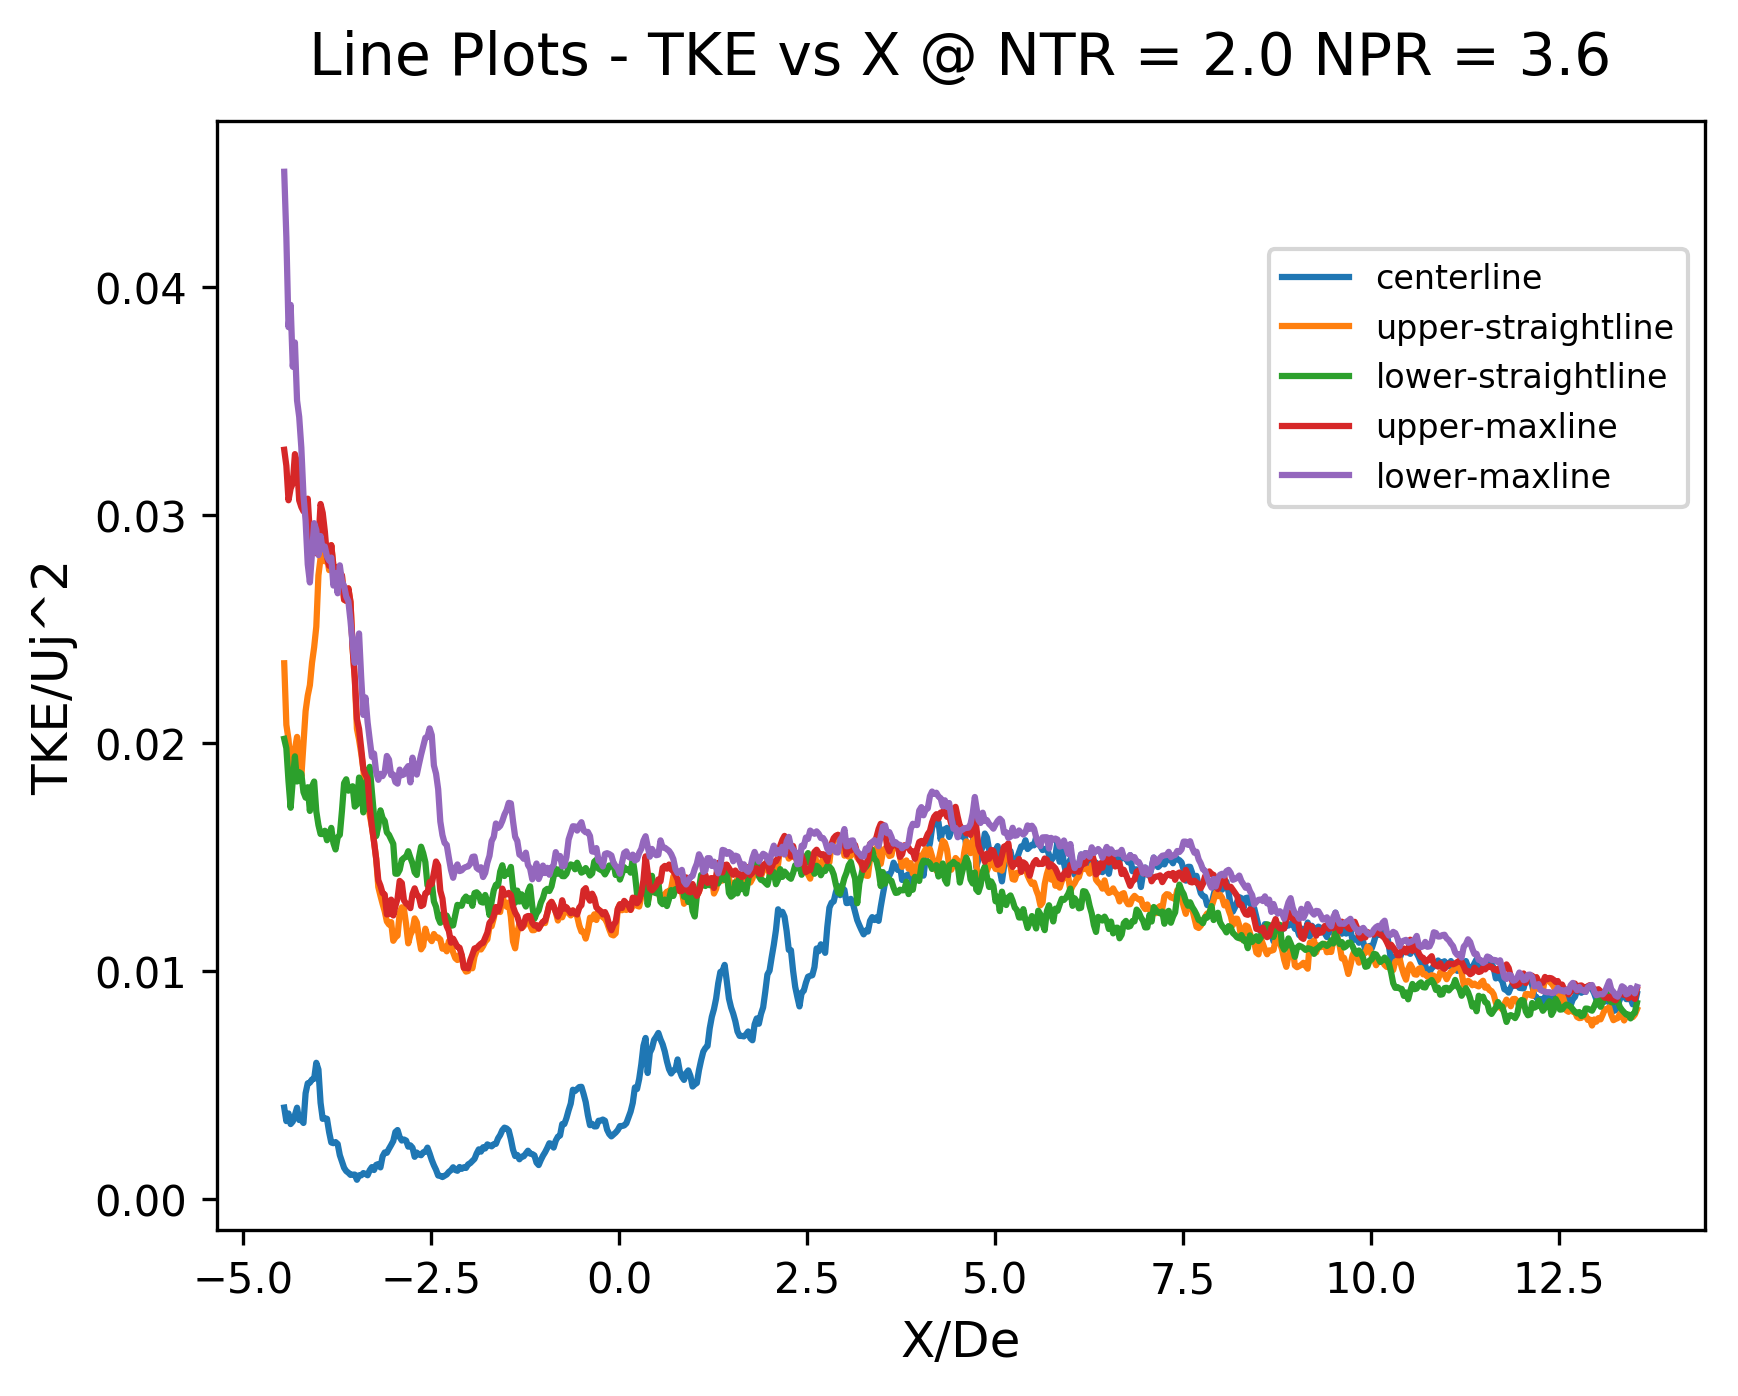
\includegraphics[width=2.5in]{images/LinePlots_TKE_NTR2p0_NPR3p6c.png}
	\caption{NTR:2p0 NPR:3p6 with chevrons}
	\label{fig:lineplotsTKE2p03p6c}
\end{subfigure}
\begin{subfigure}{.5\textwidth}
	\centering
	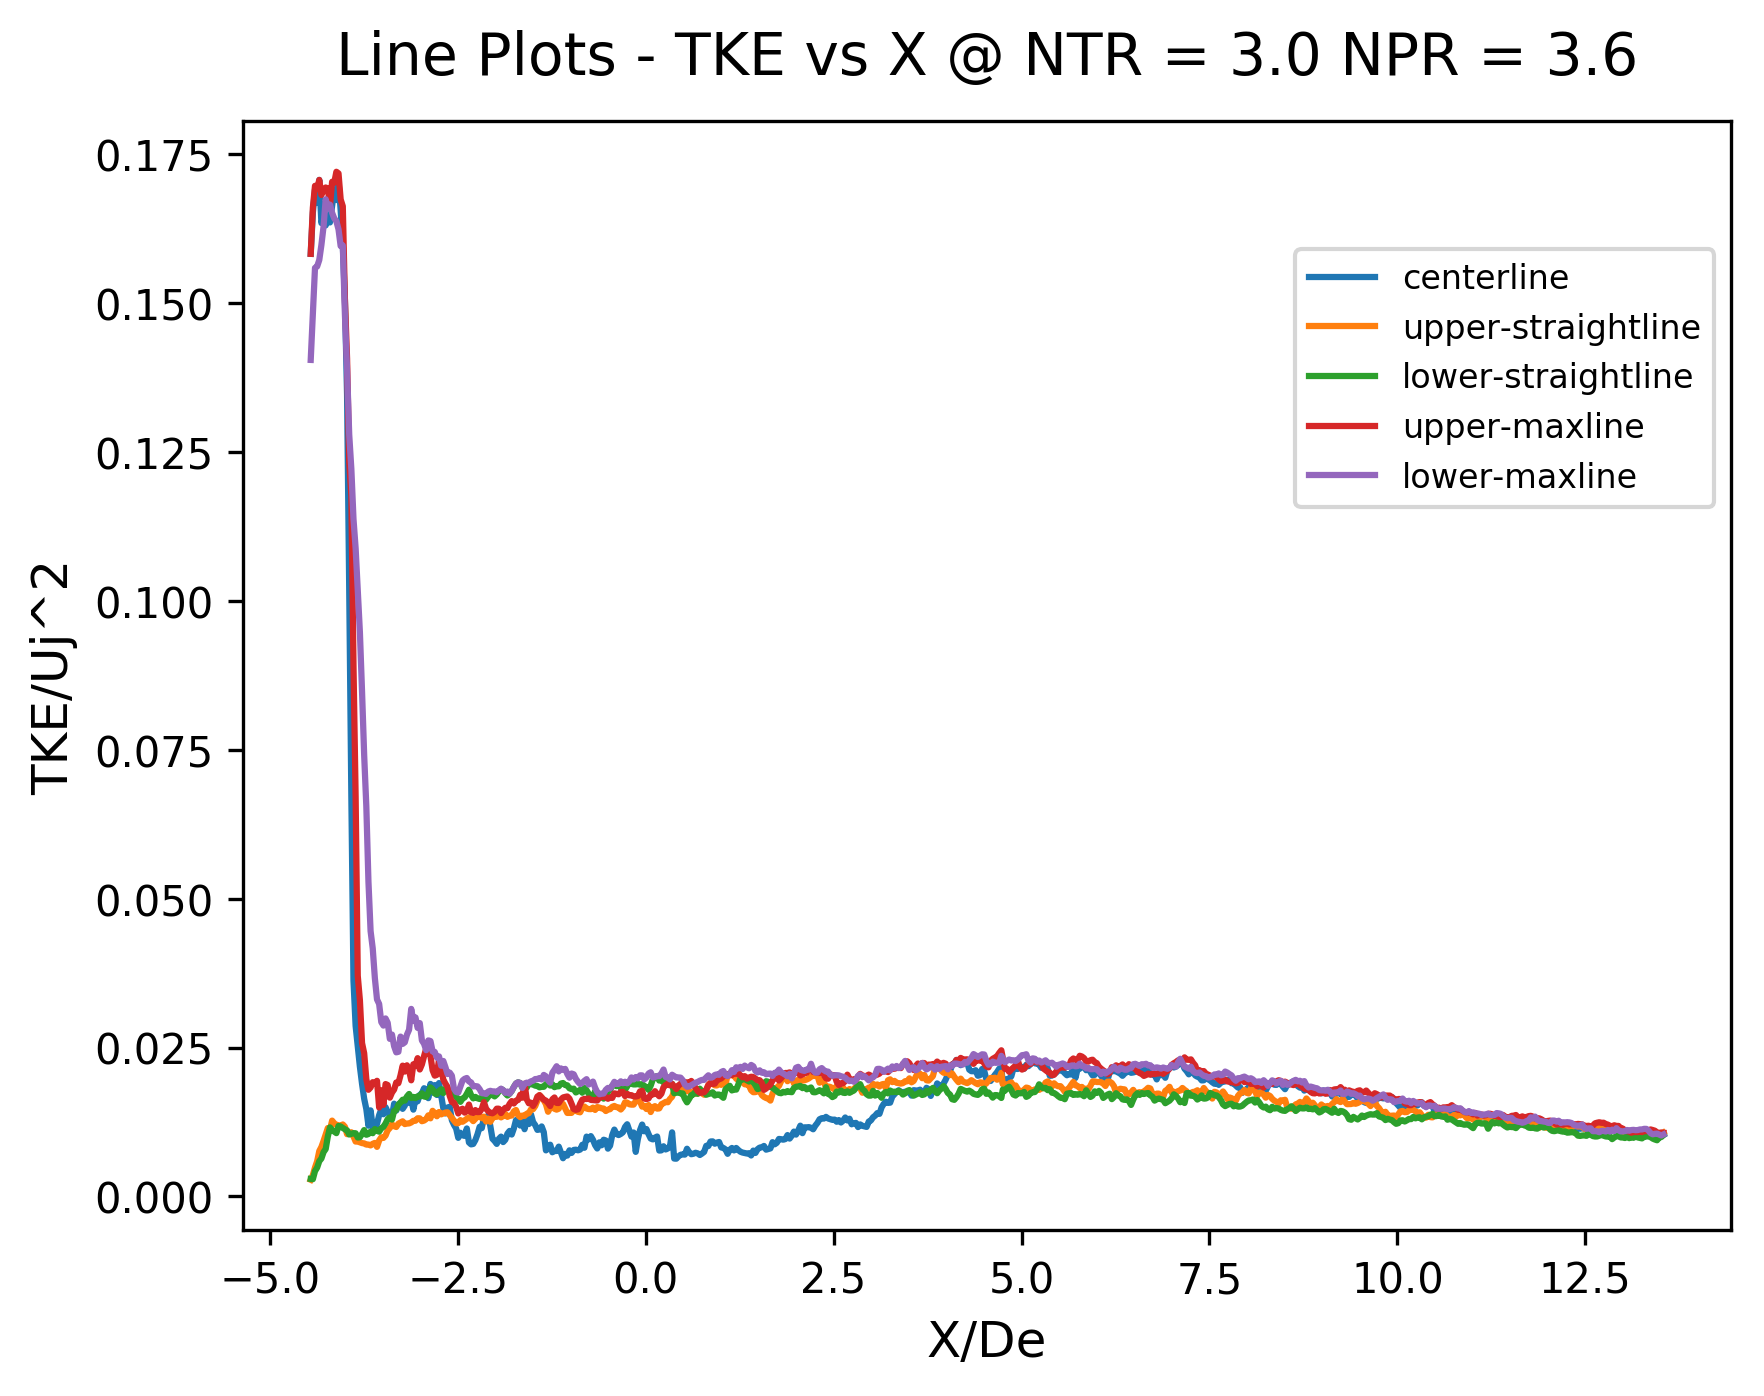
\includegraphics[width=2.5in]{images/LinePlots_TKE_NTR3p0_NPR3p6.png}
	\caption{NTR:3p0 NPR:3p6 without chevrons}
	\label{fig:lineplotsTKE3p03p6}
\end{subfigure}%
\begin{subfigure}{.5\textwidth}
	\centering
	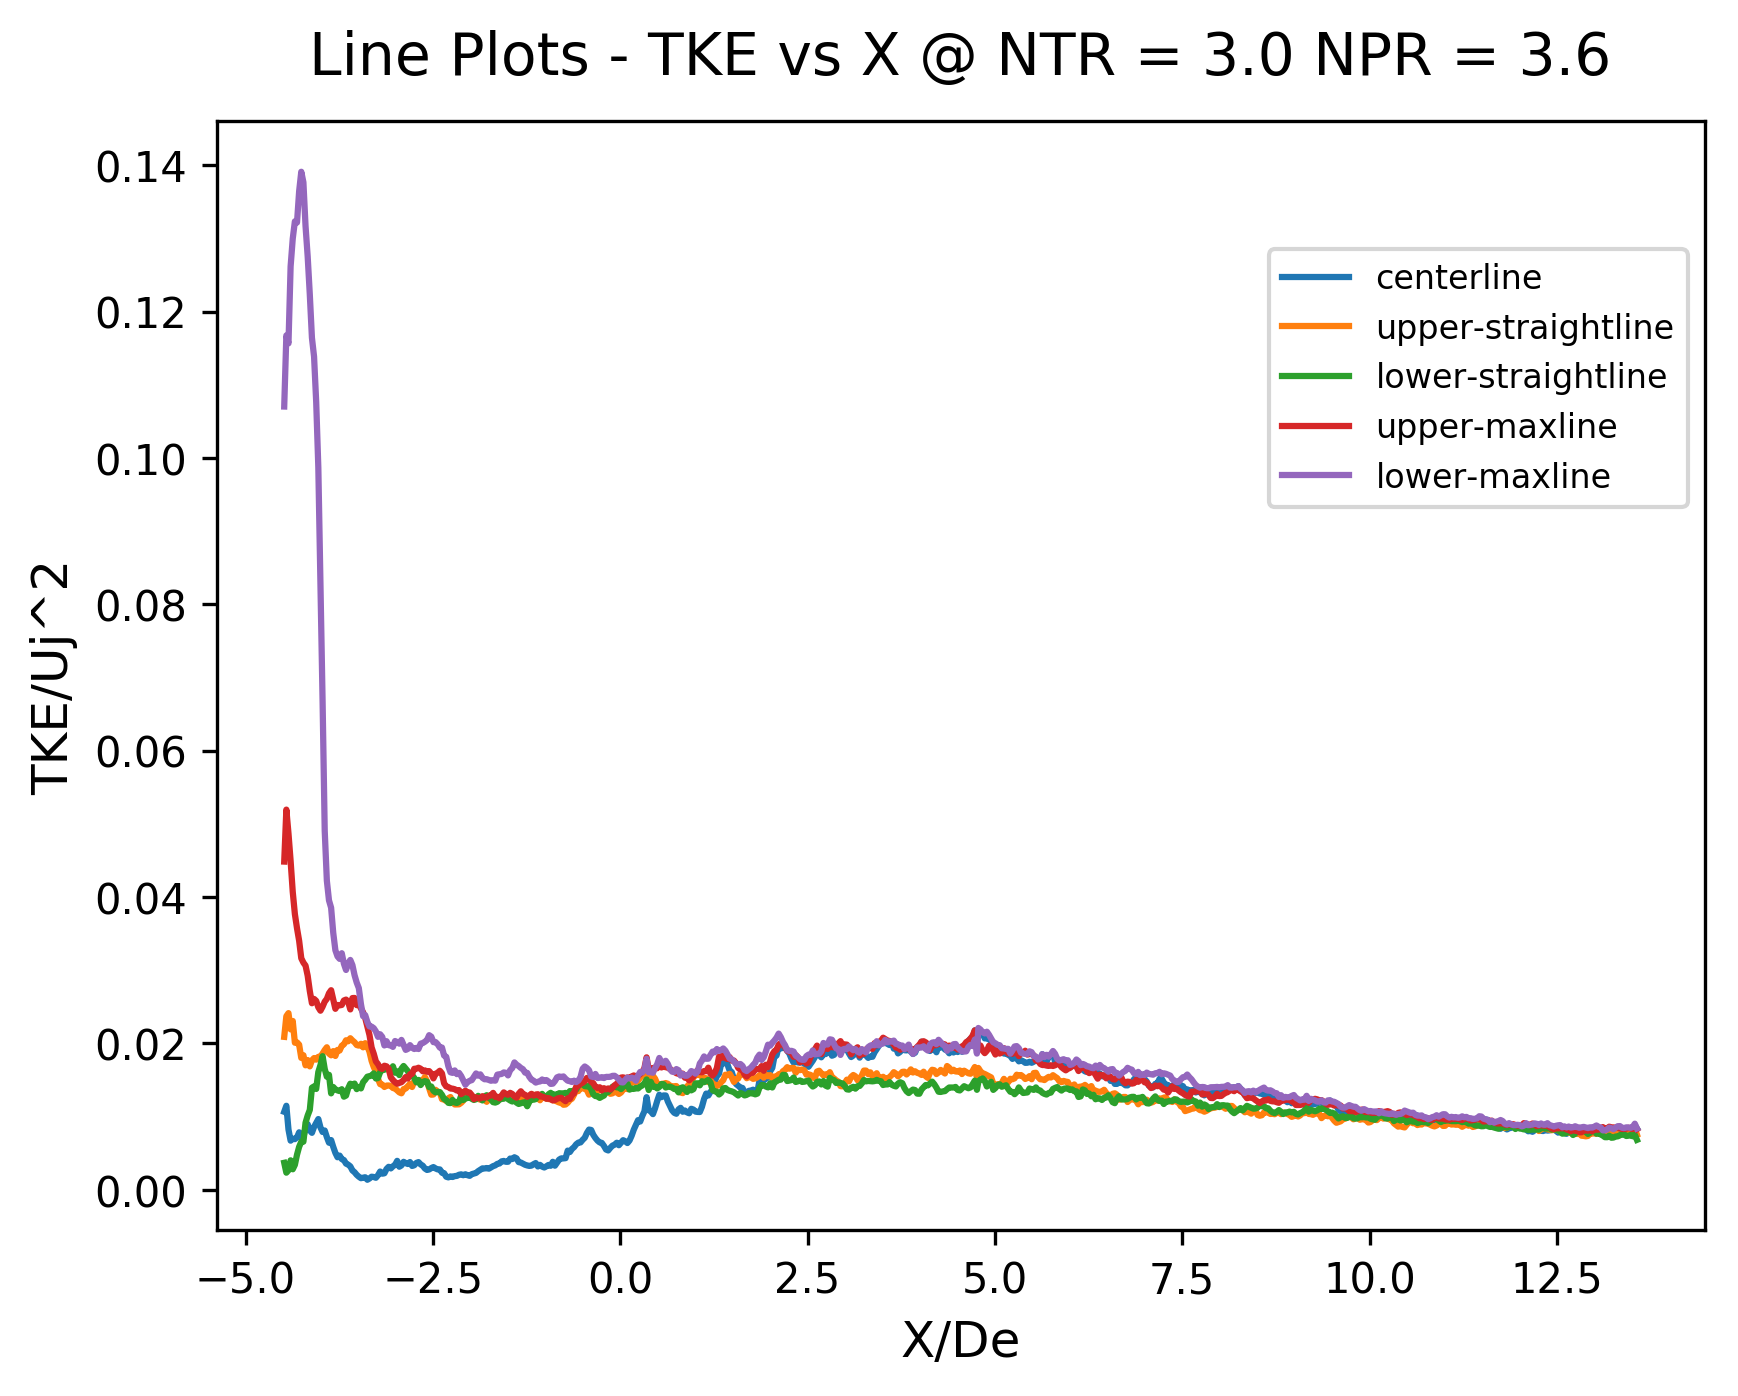
\includegraphics[width=2.5in]{images/LinePlots_TKE_NTR3p0_NPR3p6c.png}
	\caption{NTR:3p0 NPR:3p6 with chevrons}
	\label{fig:lineplotsTKE3p03p6c}
\end{subfigure}
\caption{centreline plots for TKE with and without chevrons }
\label{fig:lineplotsTKE}
\end{figure}

\section{Effect of nozzle diameter}

Fig \ref{fig:lineplotsfftb} shows that changing diameter of nozzle does not affect non-dimensionalized shock cell wavelength. But increasing diameter does seem to make distribution of shock cells slighlty more uniform as the spectrum strength is higher for larger nozzle.

\begin{figure}[H]
\begin{subfigure}{.5\textwidth}
	\centering
	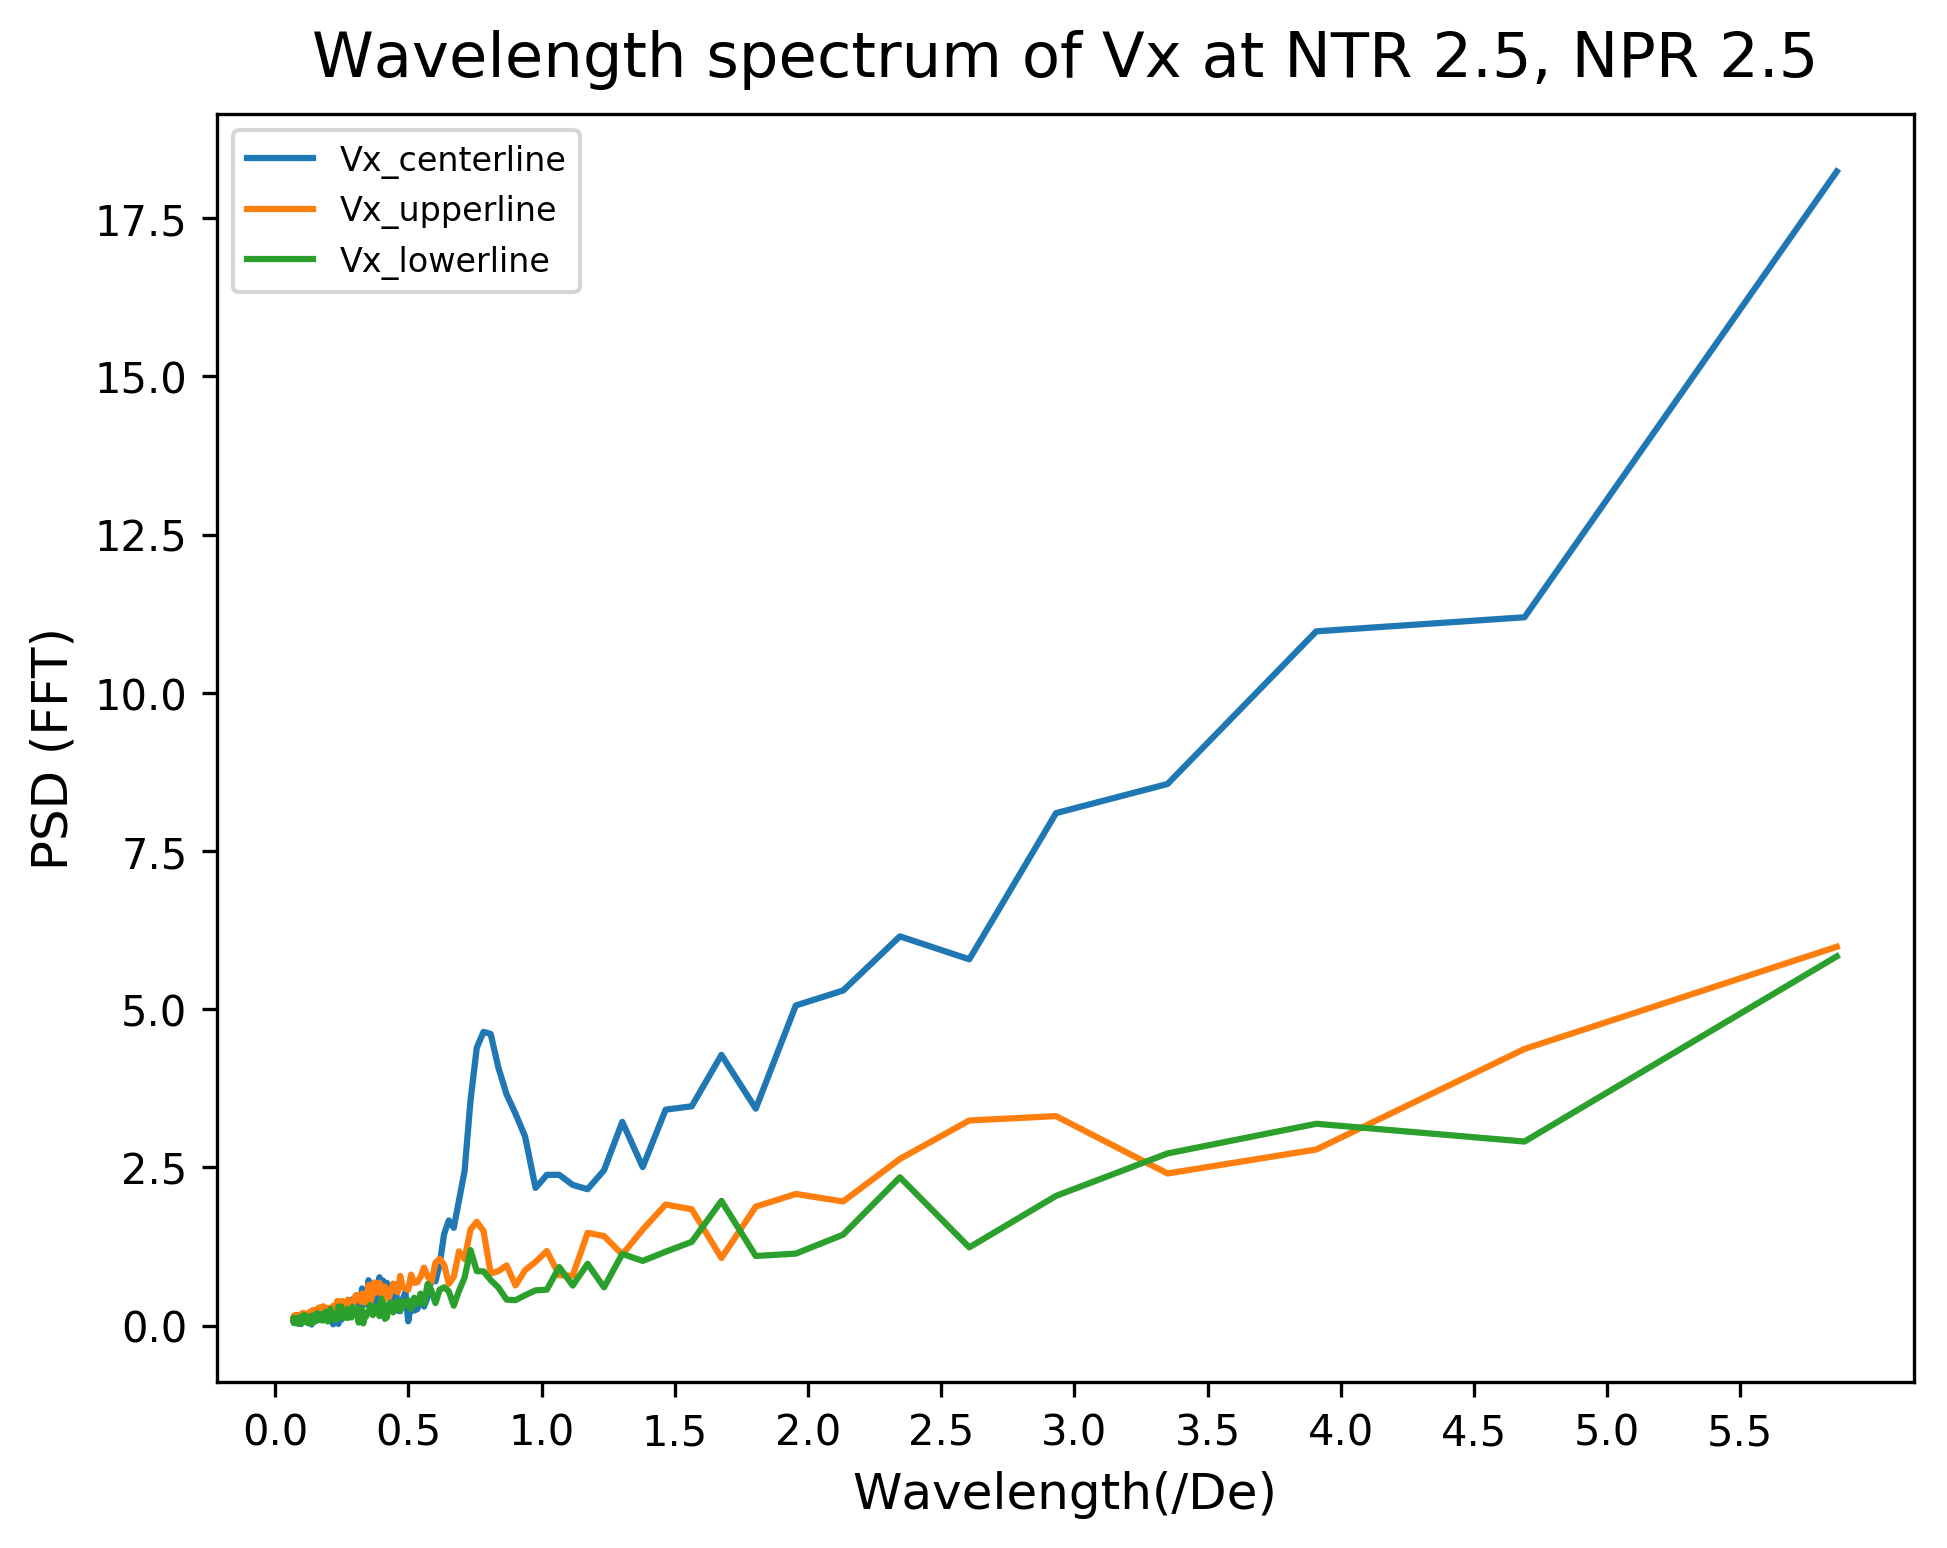
\includegraphics[width=2.5in]{images/Fft_Vx_NTR2p5_NPR2p5.png}
	\caption{NTR:2p5 NPR:2p5 - 0.813in dia }
	\label{fig:lineplotsfftb2p52p5}
\end{subfigure}%
\begin{subfigure}{.5\textwidth}
	\centering
	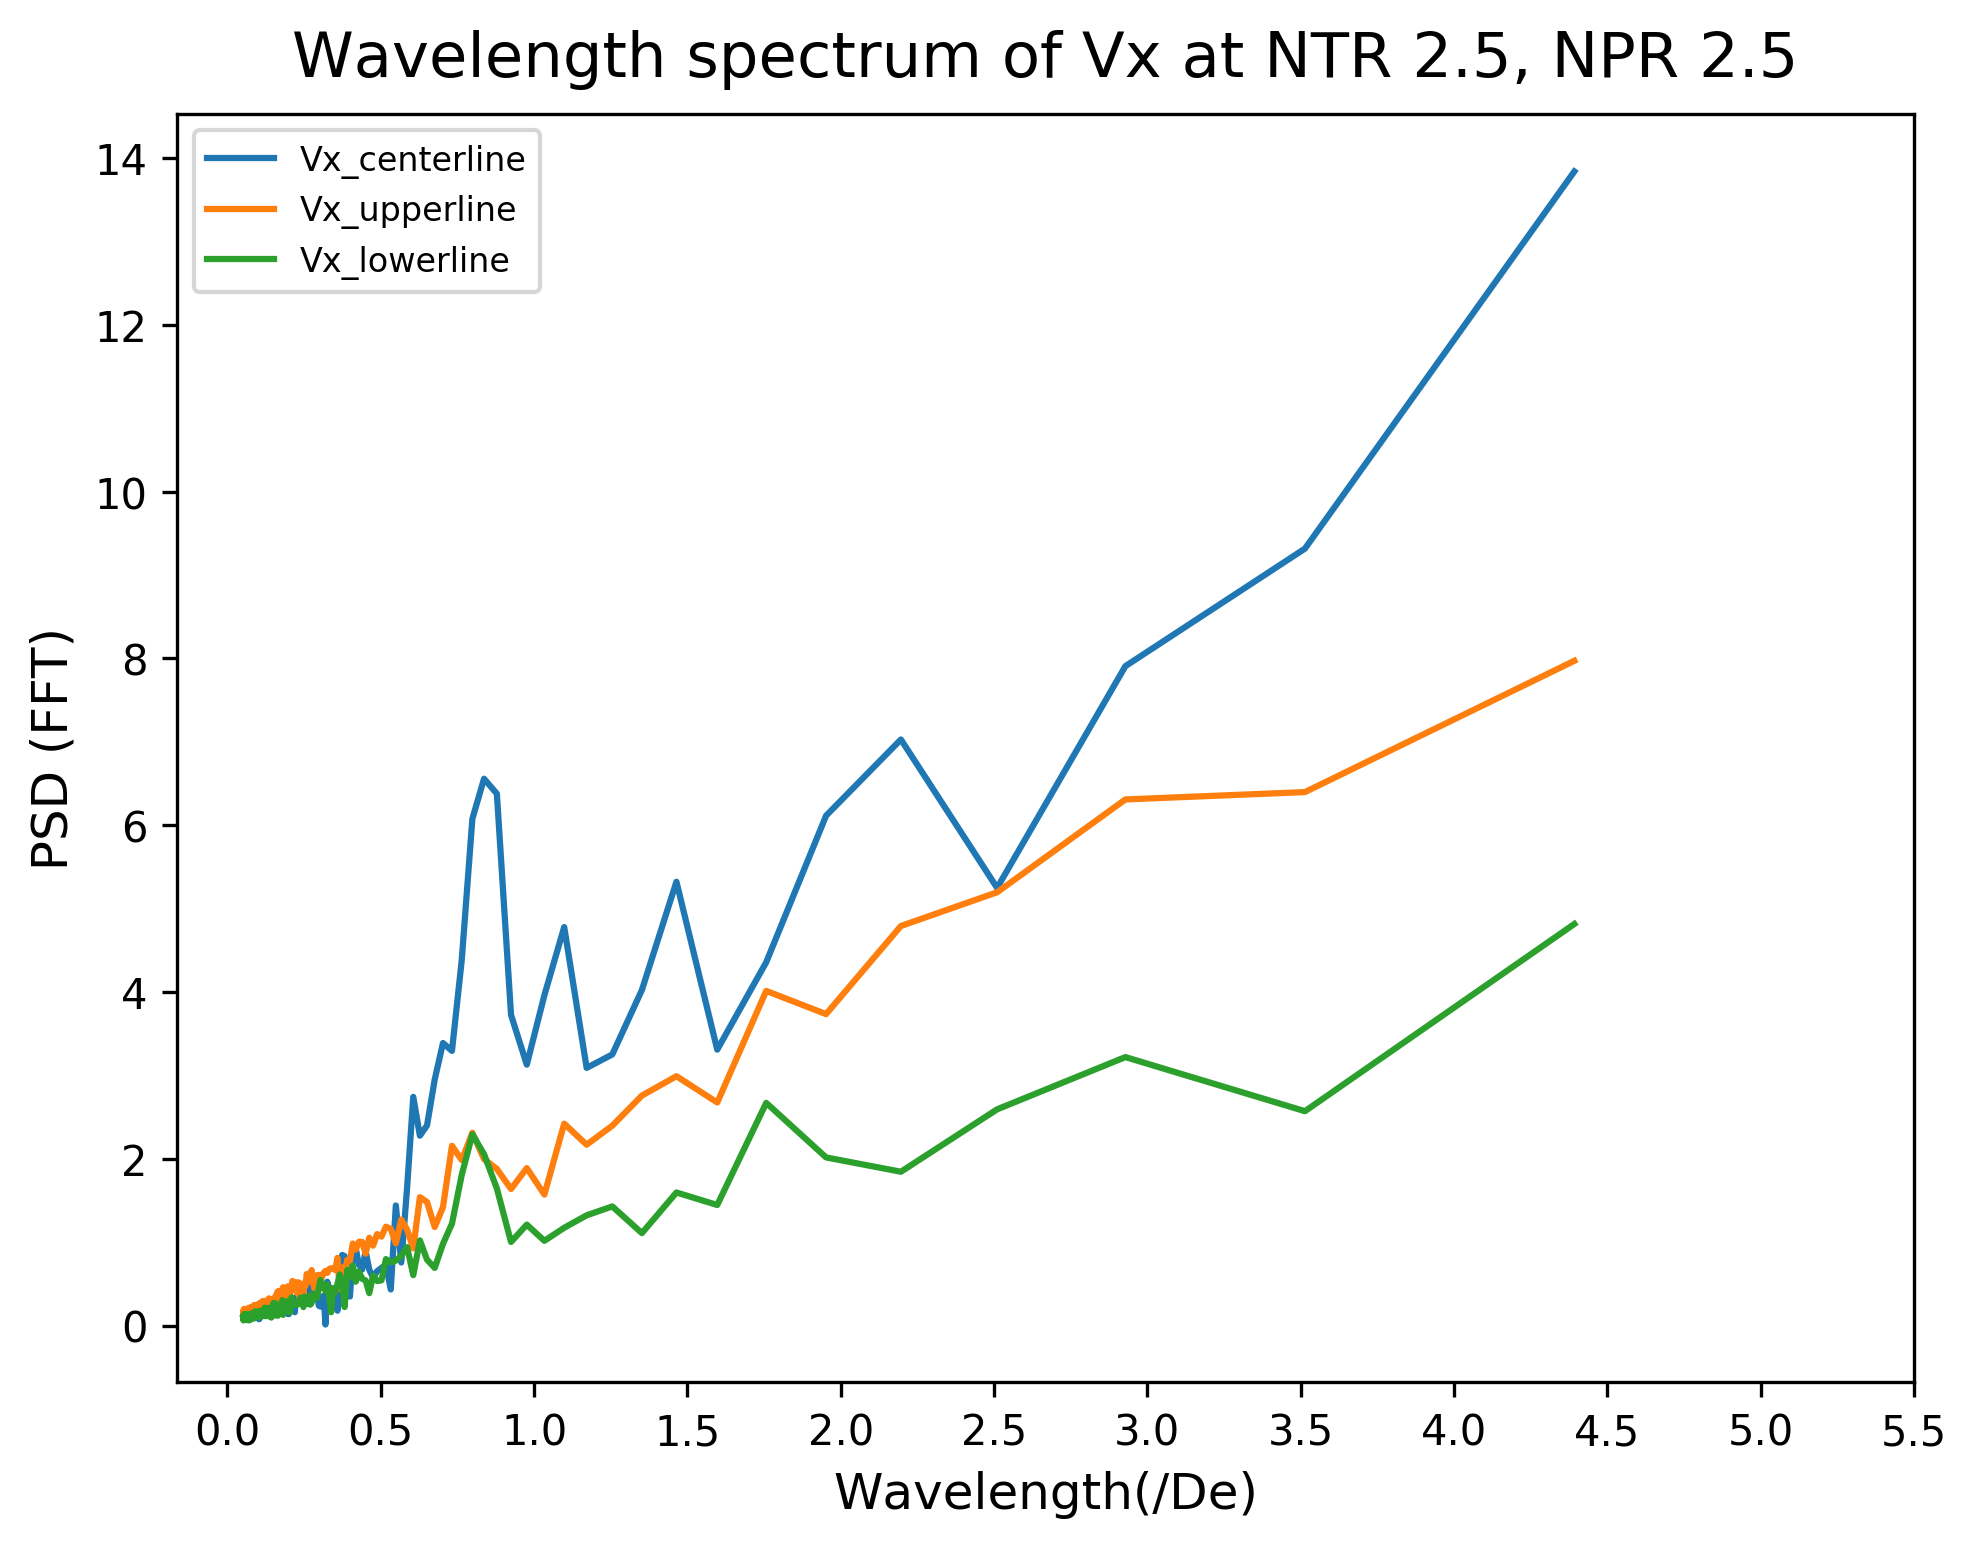
\includegraphics[width=2.5in]{images/Fft_Vx_NTR2p5_NPR2p5b.png}
	\caption{NTR:2p5 NPR:2p5 - 1.085in dia }
	\label{fig:lineplotsfft2p52p5b}
\end{subfigure}
\begin{subfigure}{.5\textwidth}
	\centering
	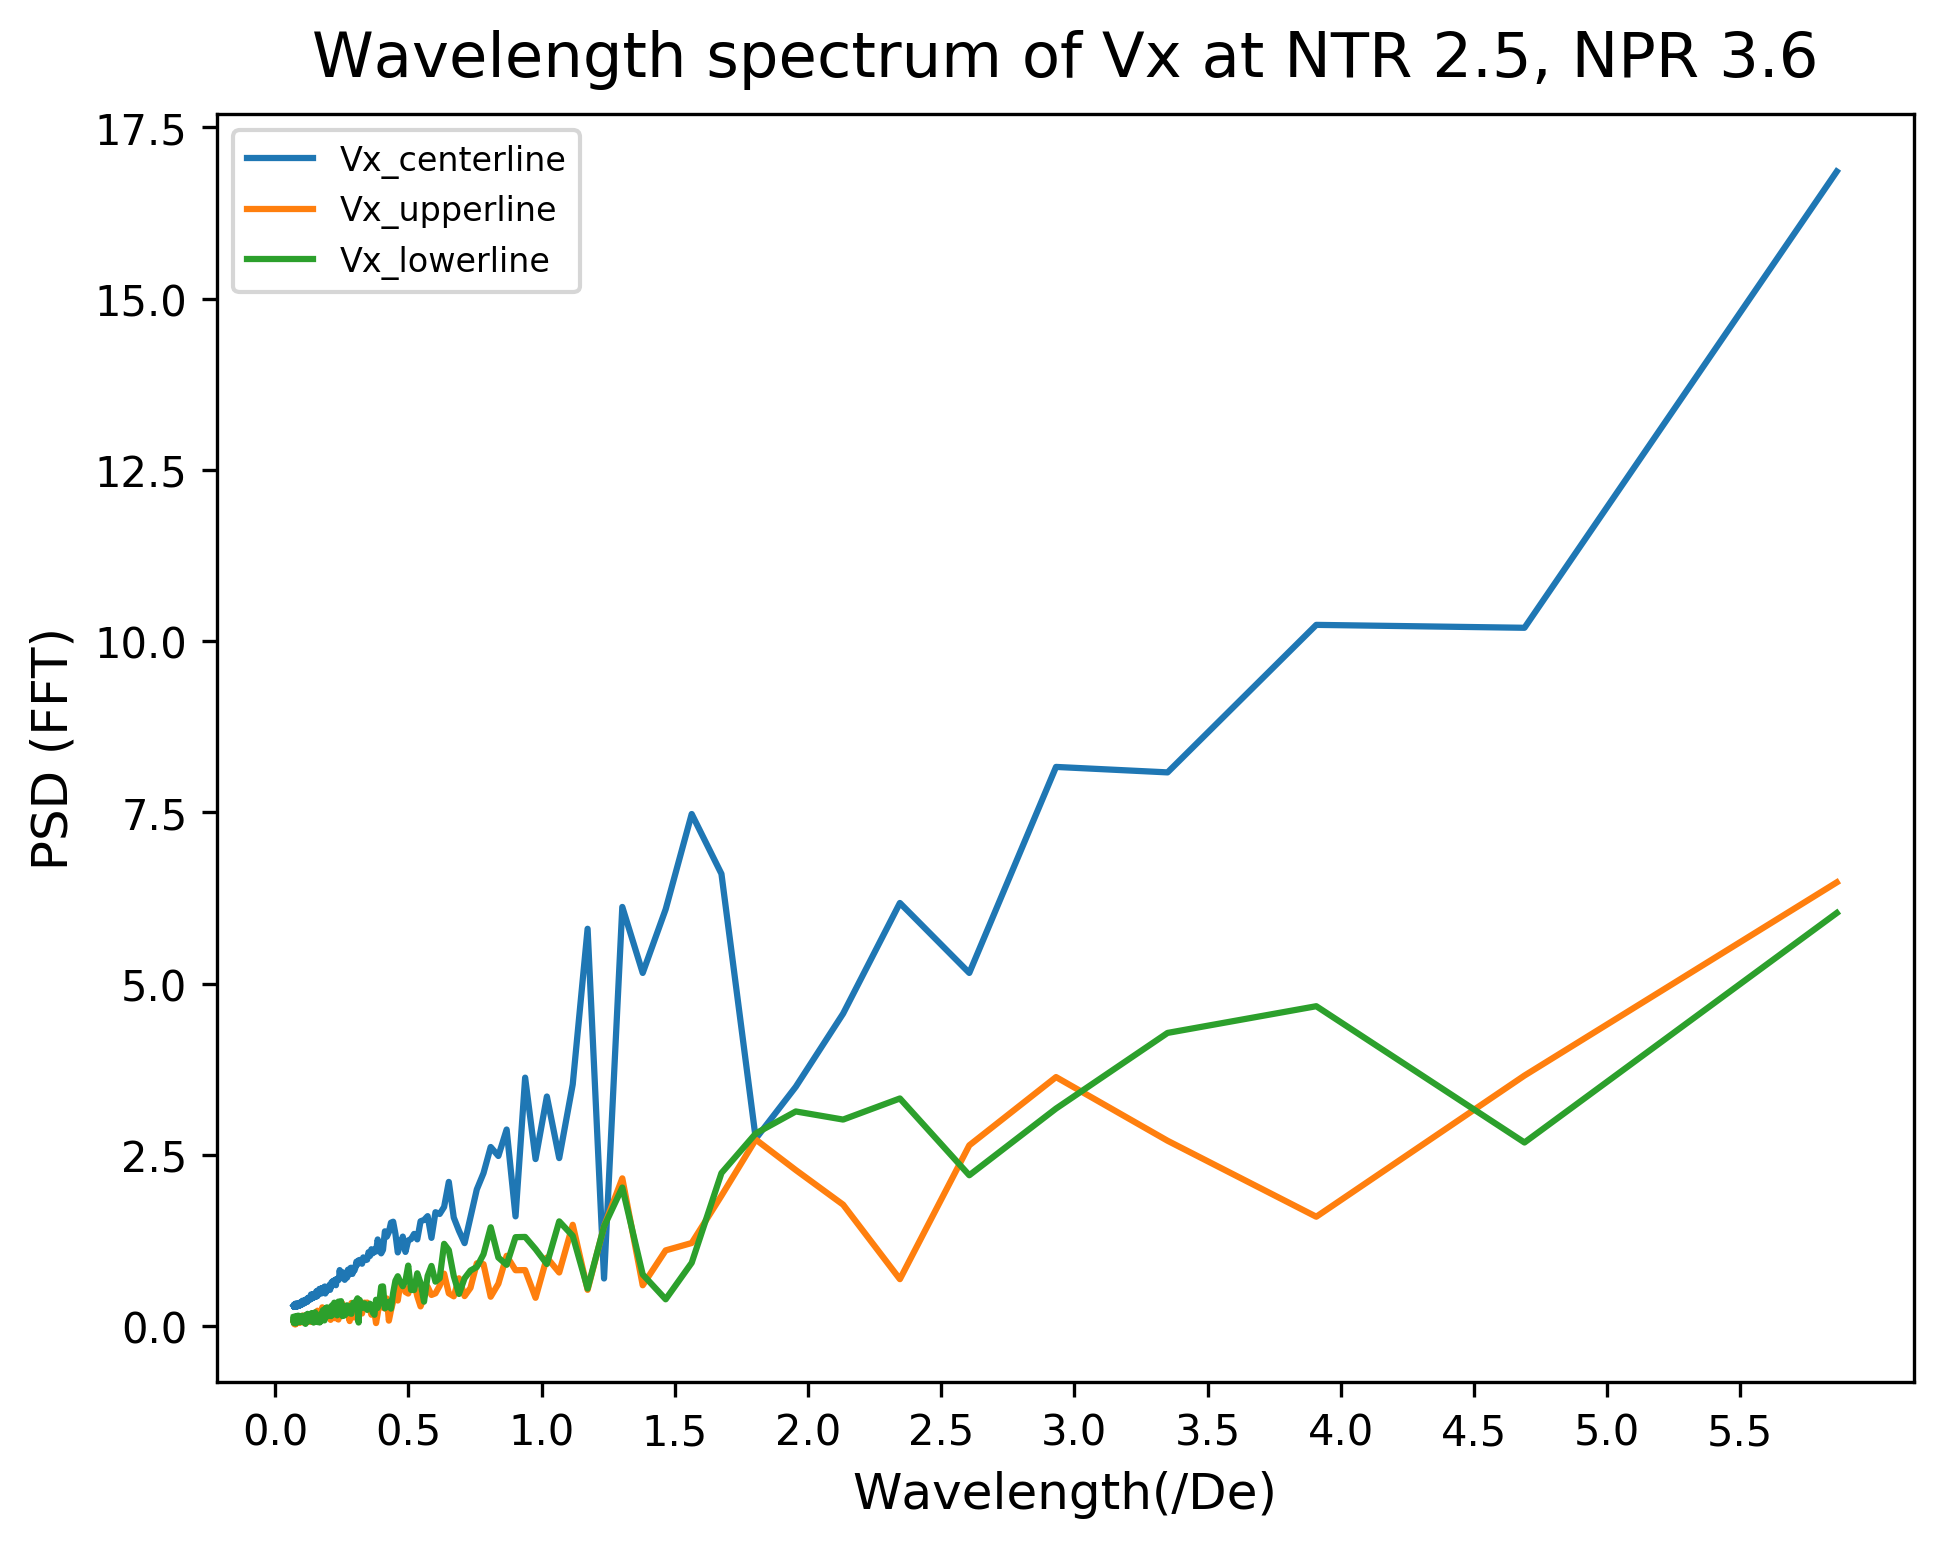
\includegraphics[width=2.5in]{images/Fft_Vx_NTR2p5_NPR3p6.png}
	\caption{NTR:2p5 NPR:3p6 - 0.813in dia}
	\label{fig:lineplotsfftb2p53p6}
\end{subfigure}%
\begin{subfigure}{.5\textwidth}
	\centering
	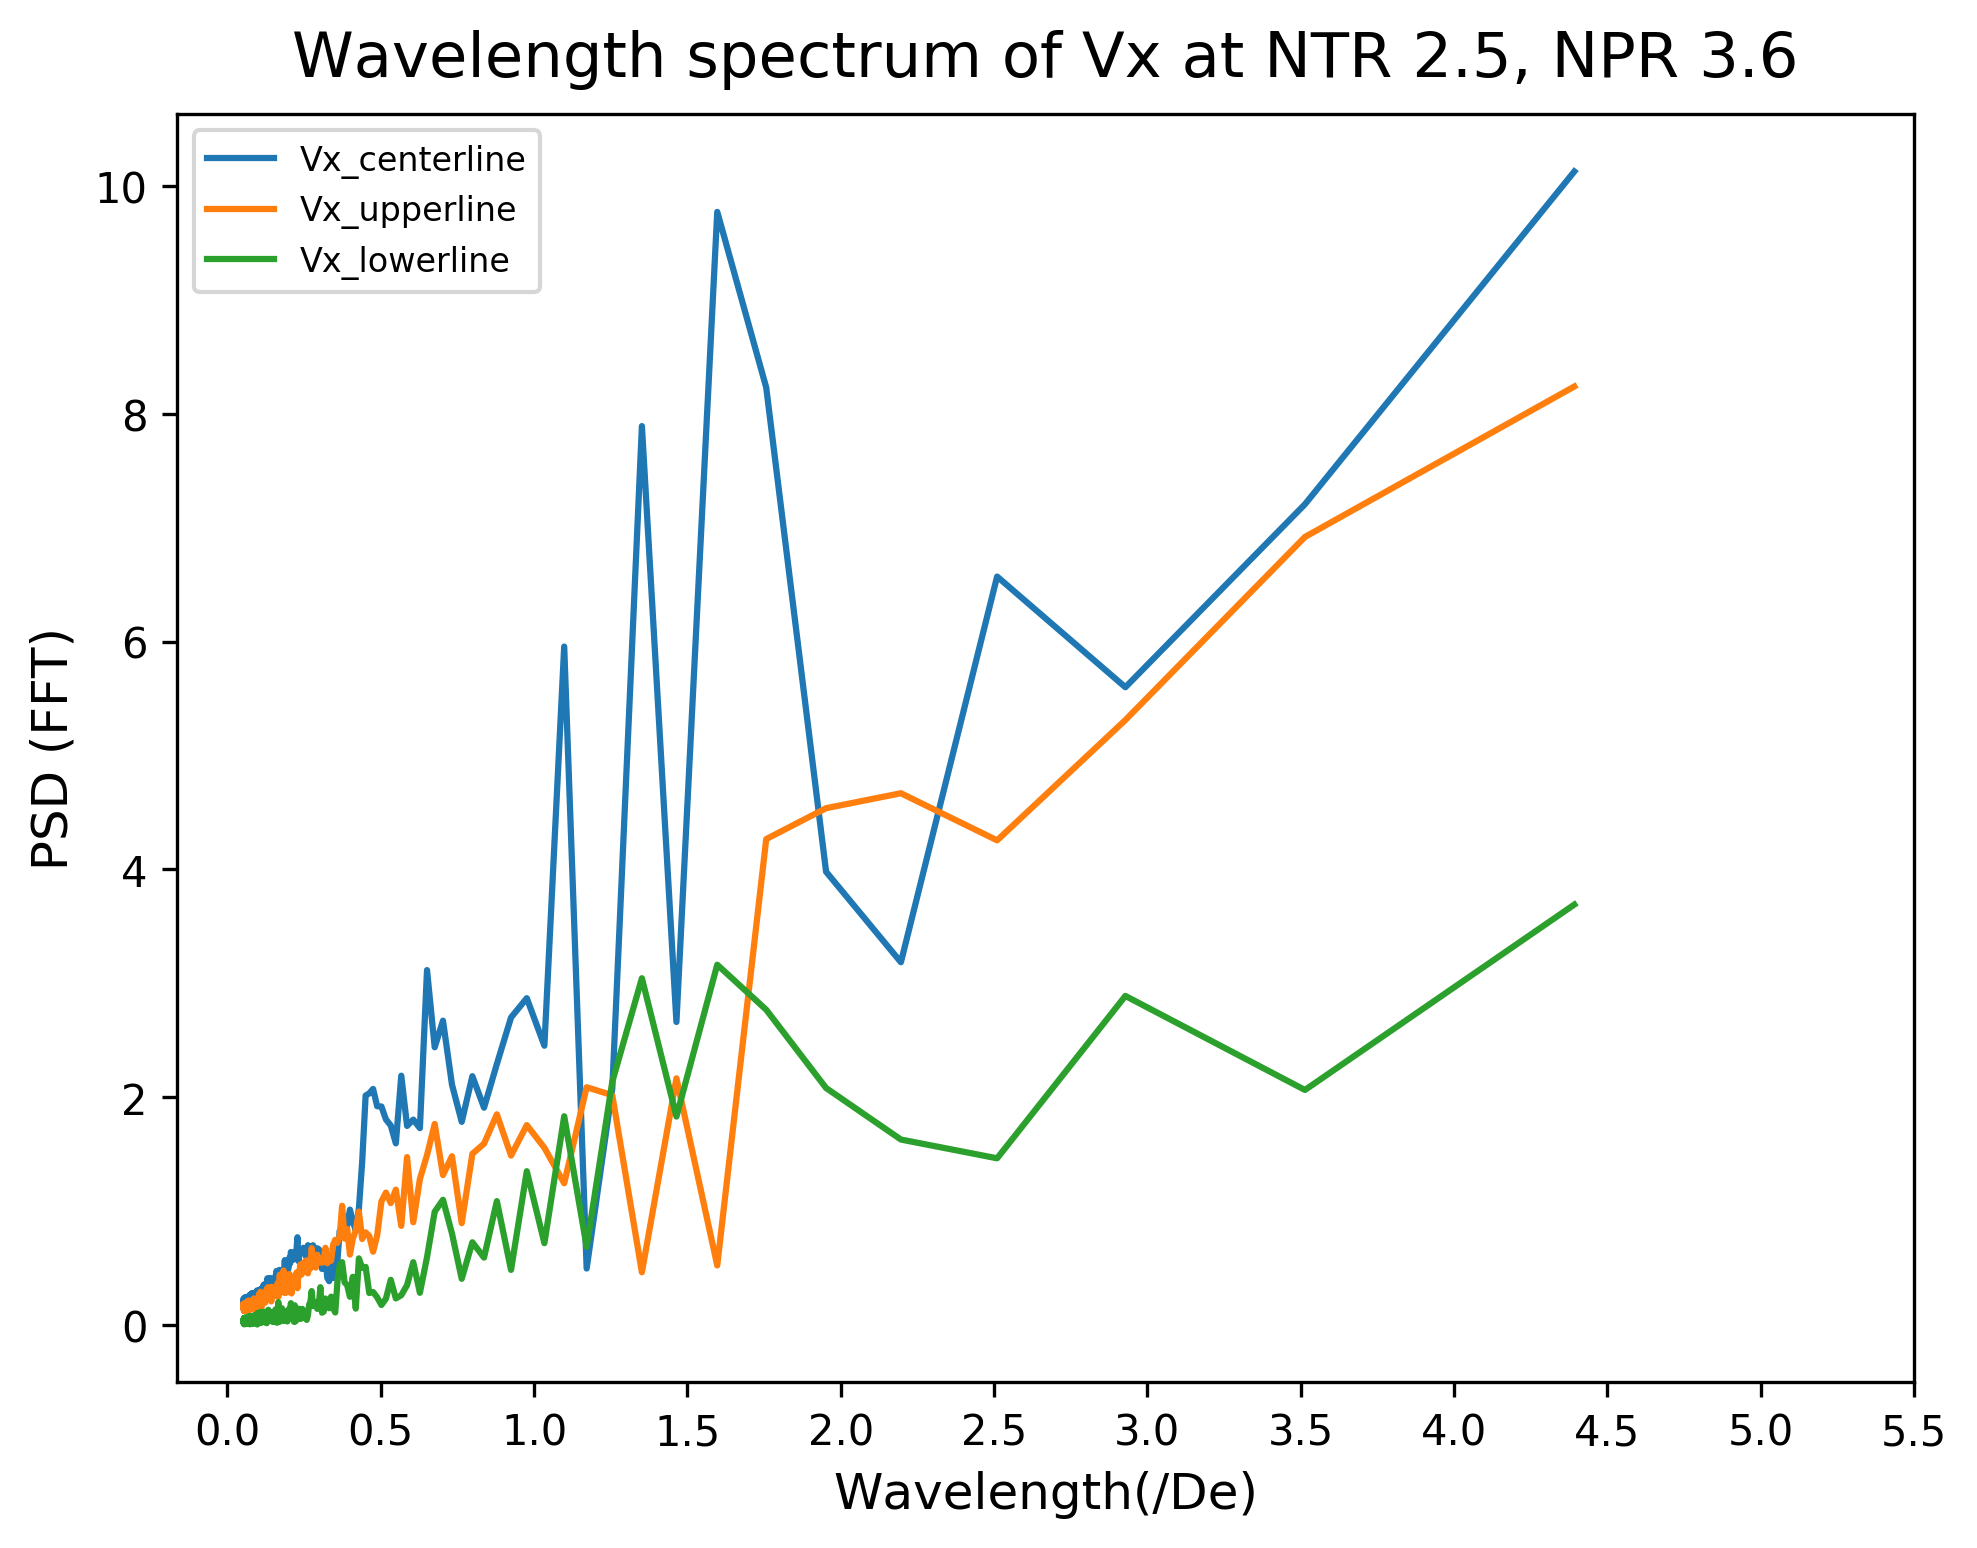
\includegraphics[width=2.5in]{images/Fft_Vx_NTR2p5_NPR3p6b.png}
	\caption{NTR:2p5 NPR:3p6 - 1.085in dia}
	\label{fig:lineplotsfftb2p53p6b}
\end{subfigure}
\begin{subfigure}{.5\textwidth}
	\centering
	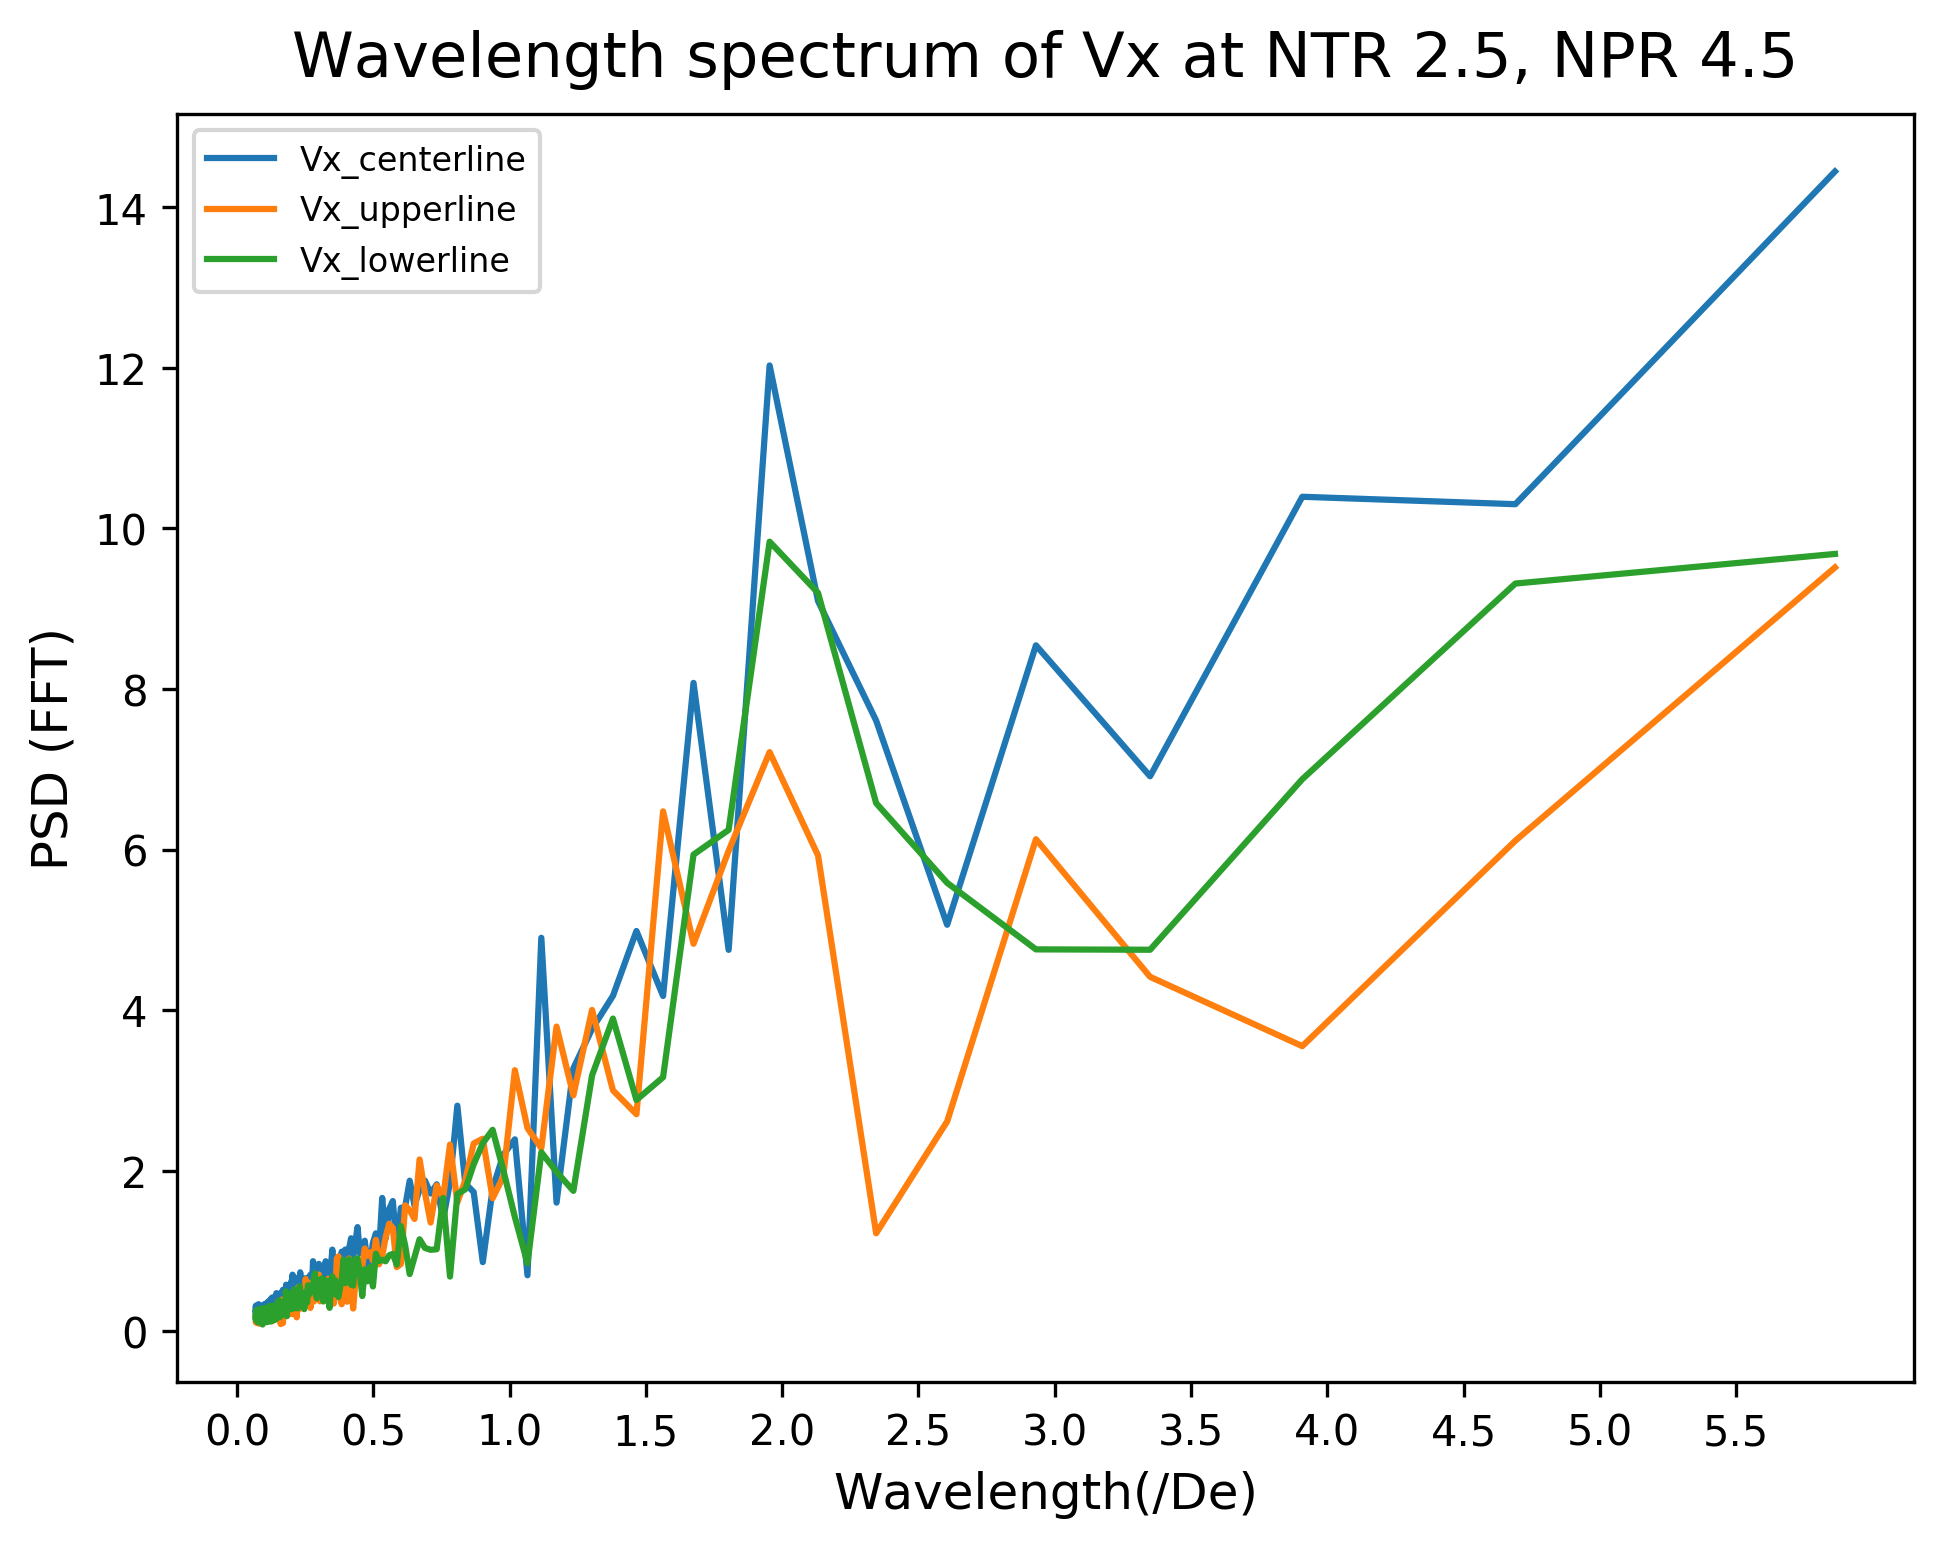
\includegraphics[width=2.5in]{images/Fft_Vx_NTR2p5_NPR4p5.png}
	\caption{NTR:2p5 NPR:4p5 - 0.813in dia}
	\label{fig:lineplotsfftb2p54p5}
\end{subfigure}%
\begin{subfigure}{.5\textwidth}
	\centering
	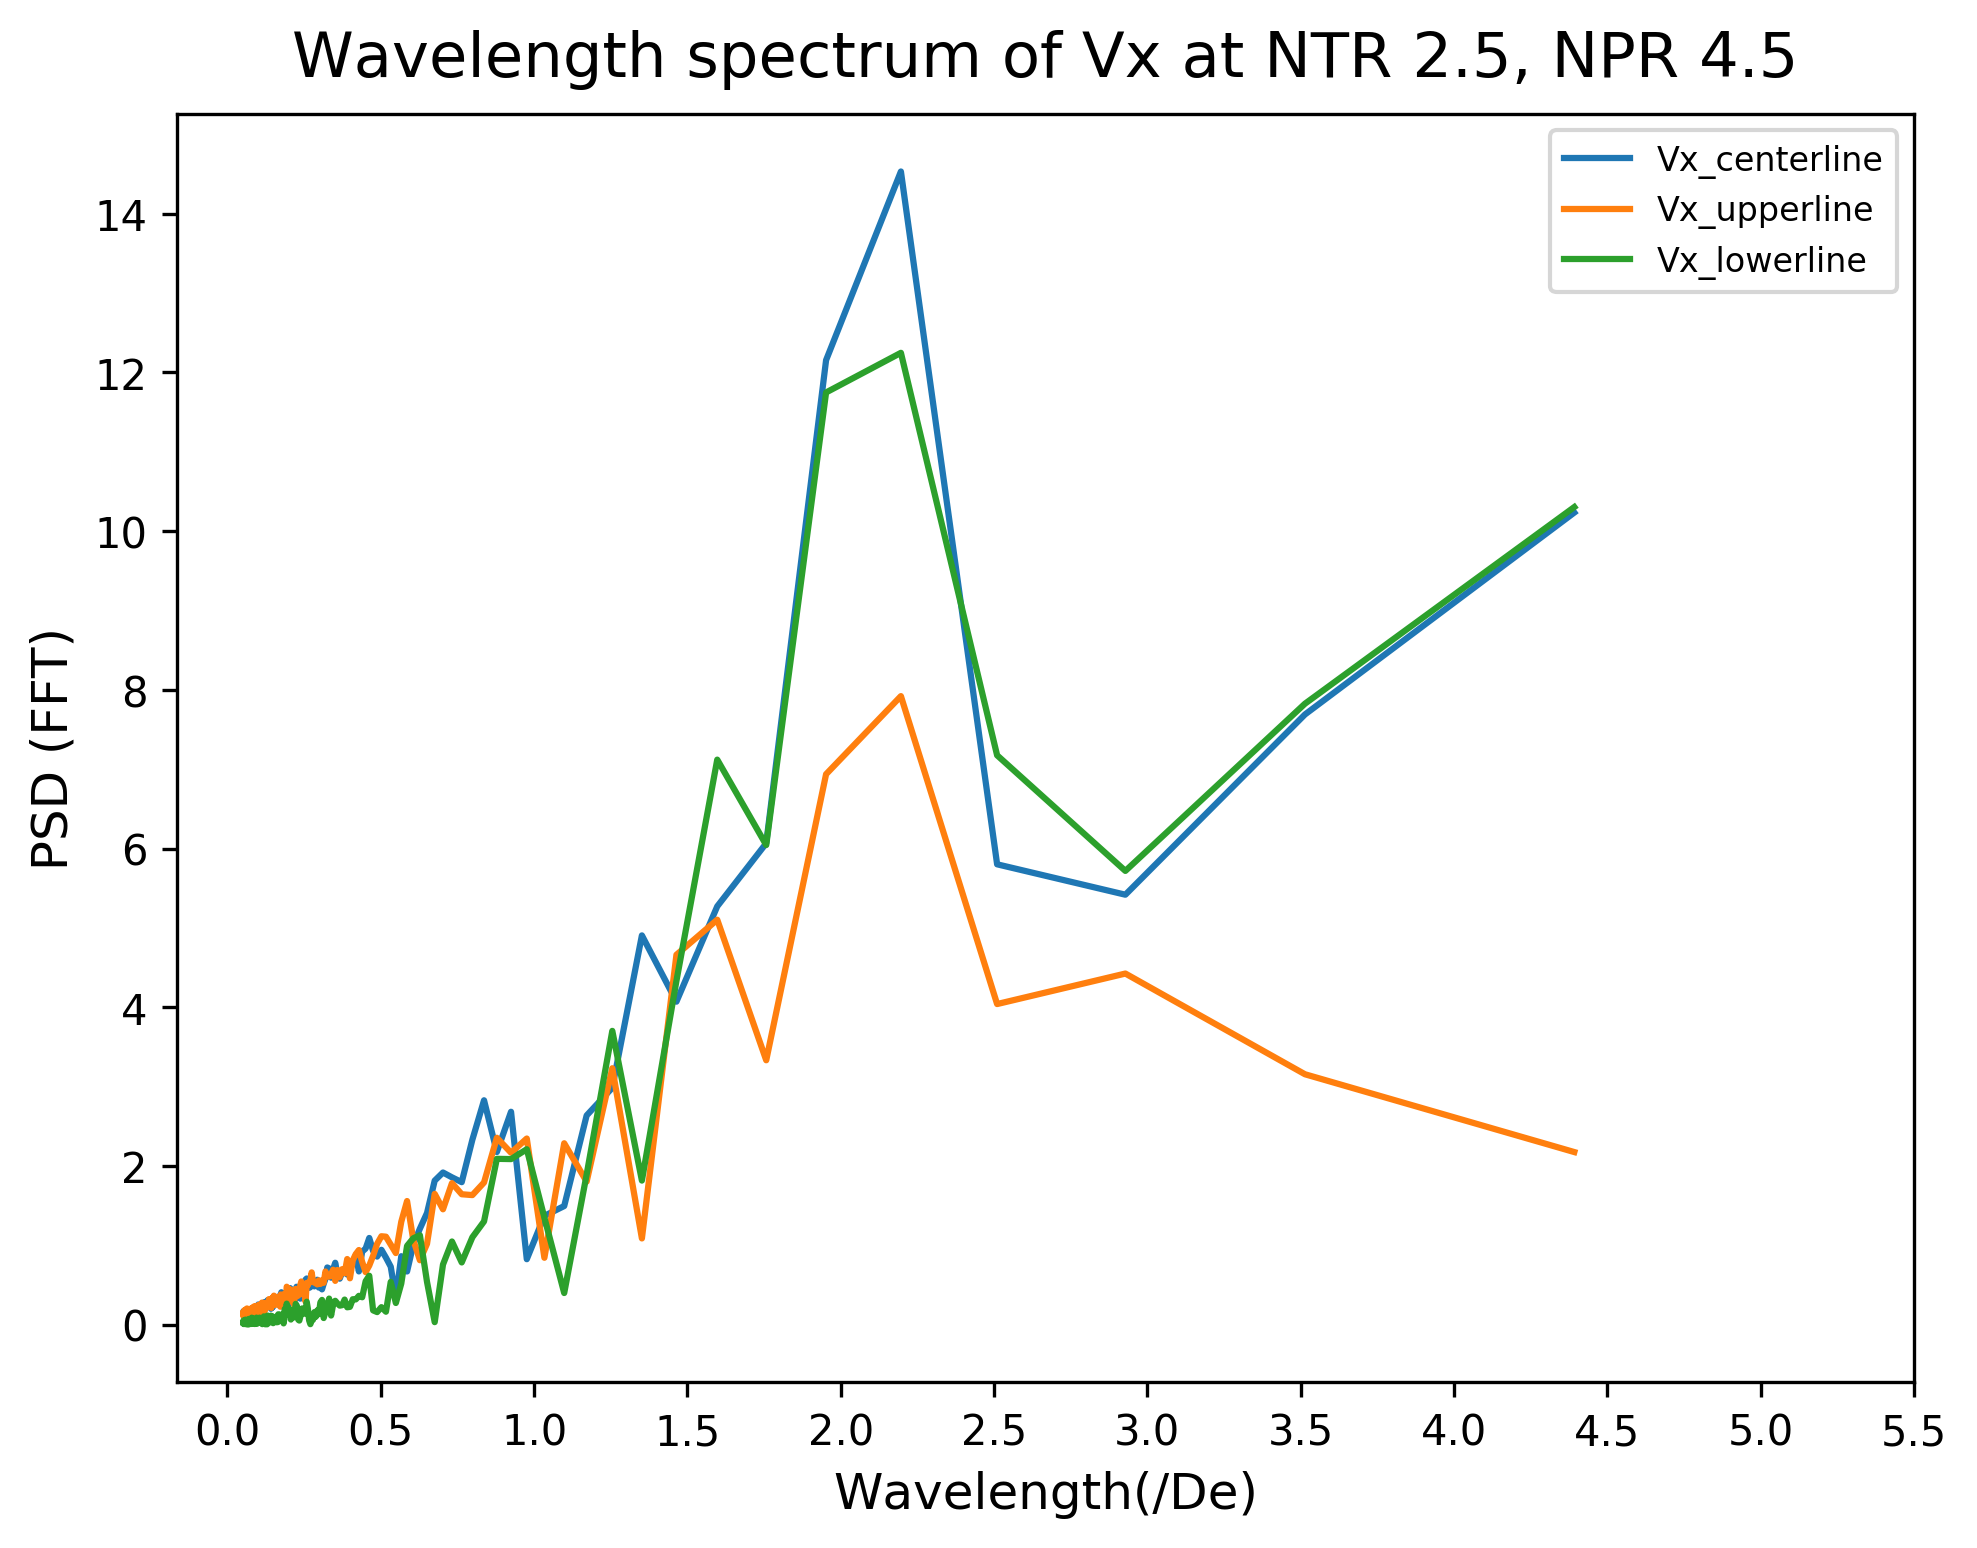
\includegraphics[width=2.5in]{images/Fft_Vx_NTR2p5_NPR4p5b.png}
	\caption{NTR:2p5 NPR:4p5 - 1.085in dia}
	\label{fig:lineplotsfftb2p54p5b}
\end{subfigure}
\caption{FFT of centreline plots for Vx with dia 0.813in and 1.085in }
\label{fig:lineplotsfftb}
\end{figure}

Interestingly, Non-dimensionalized length of potential core (fig \ref{fig:lineplotsTKEb}), is not constant anymore. Larger nozzle has more than 50\% higher core length than smaller nozzle consistently for various pressures (diameter ratio of nozzles is 1.33). This could be because of disproportionate dependence of various properties on length scales. It could also have something to do with the cascading of flow structures into small components which are no longer related to the scales of geometry so that spreading of shear layer or turbulence is less reliant on jet velocity.

\begin{figure}[H]
\begin{subfigure}{.5\textwidth}
	\centering
	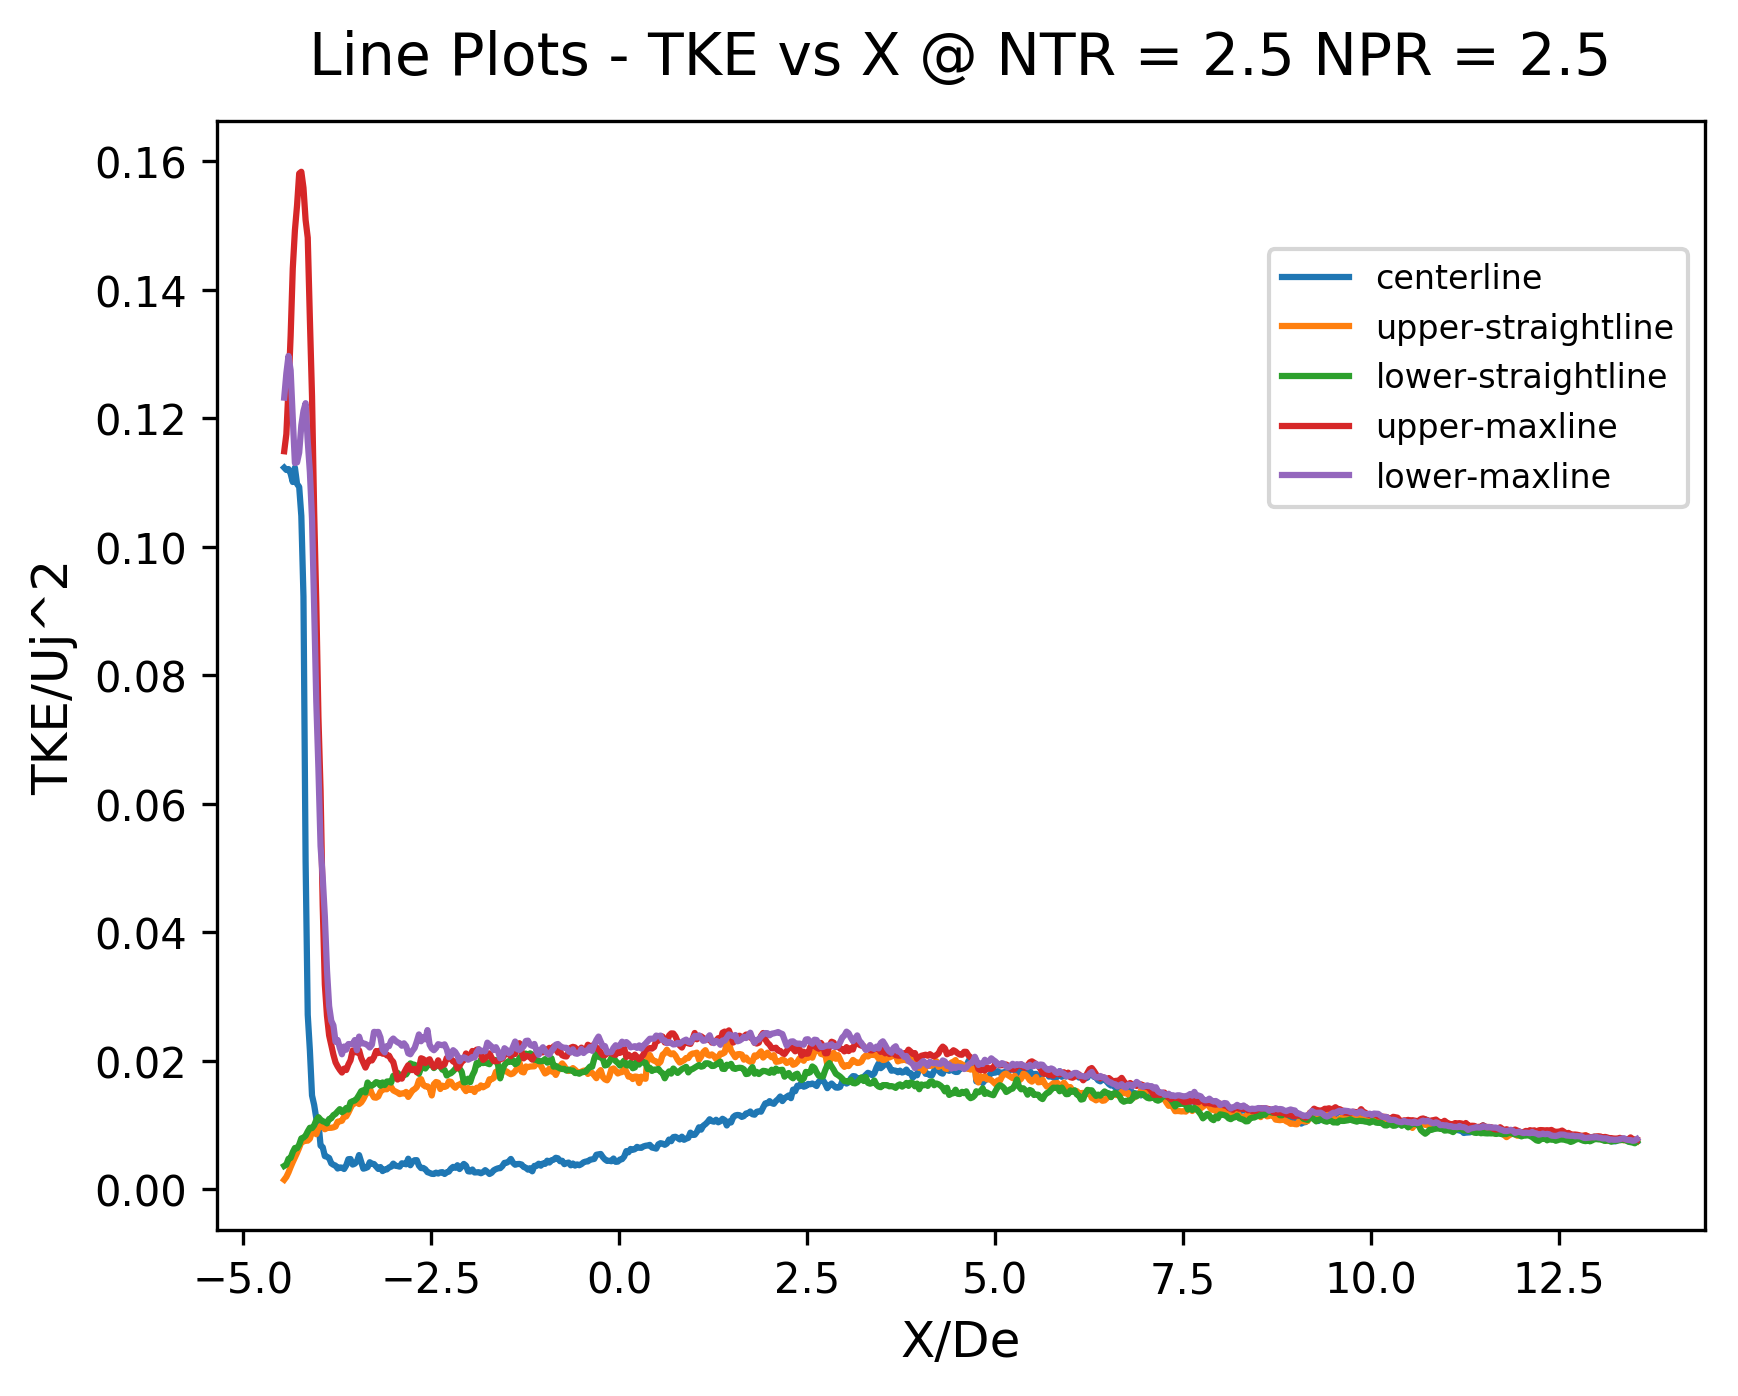
\includegraphics[width=2.5in]{images/LinePlots_TKE_NTR2p5_NPR2p5.png}
	\caption{NTR:2p5 NPR:2p5 - 0.813in dia }
	\label{fig:lineplotsTKEb2p52p5}
\end{subfigure}%
\begin{subfigure}{.5\textwidth}
	\centering
	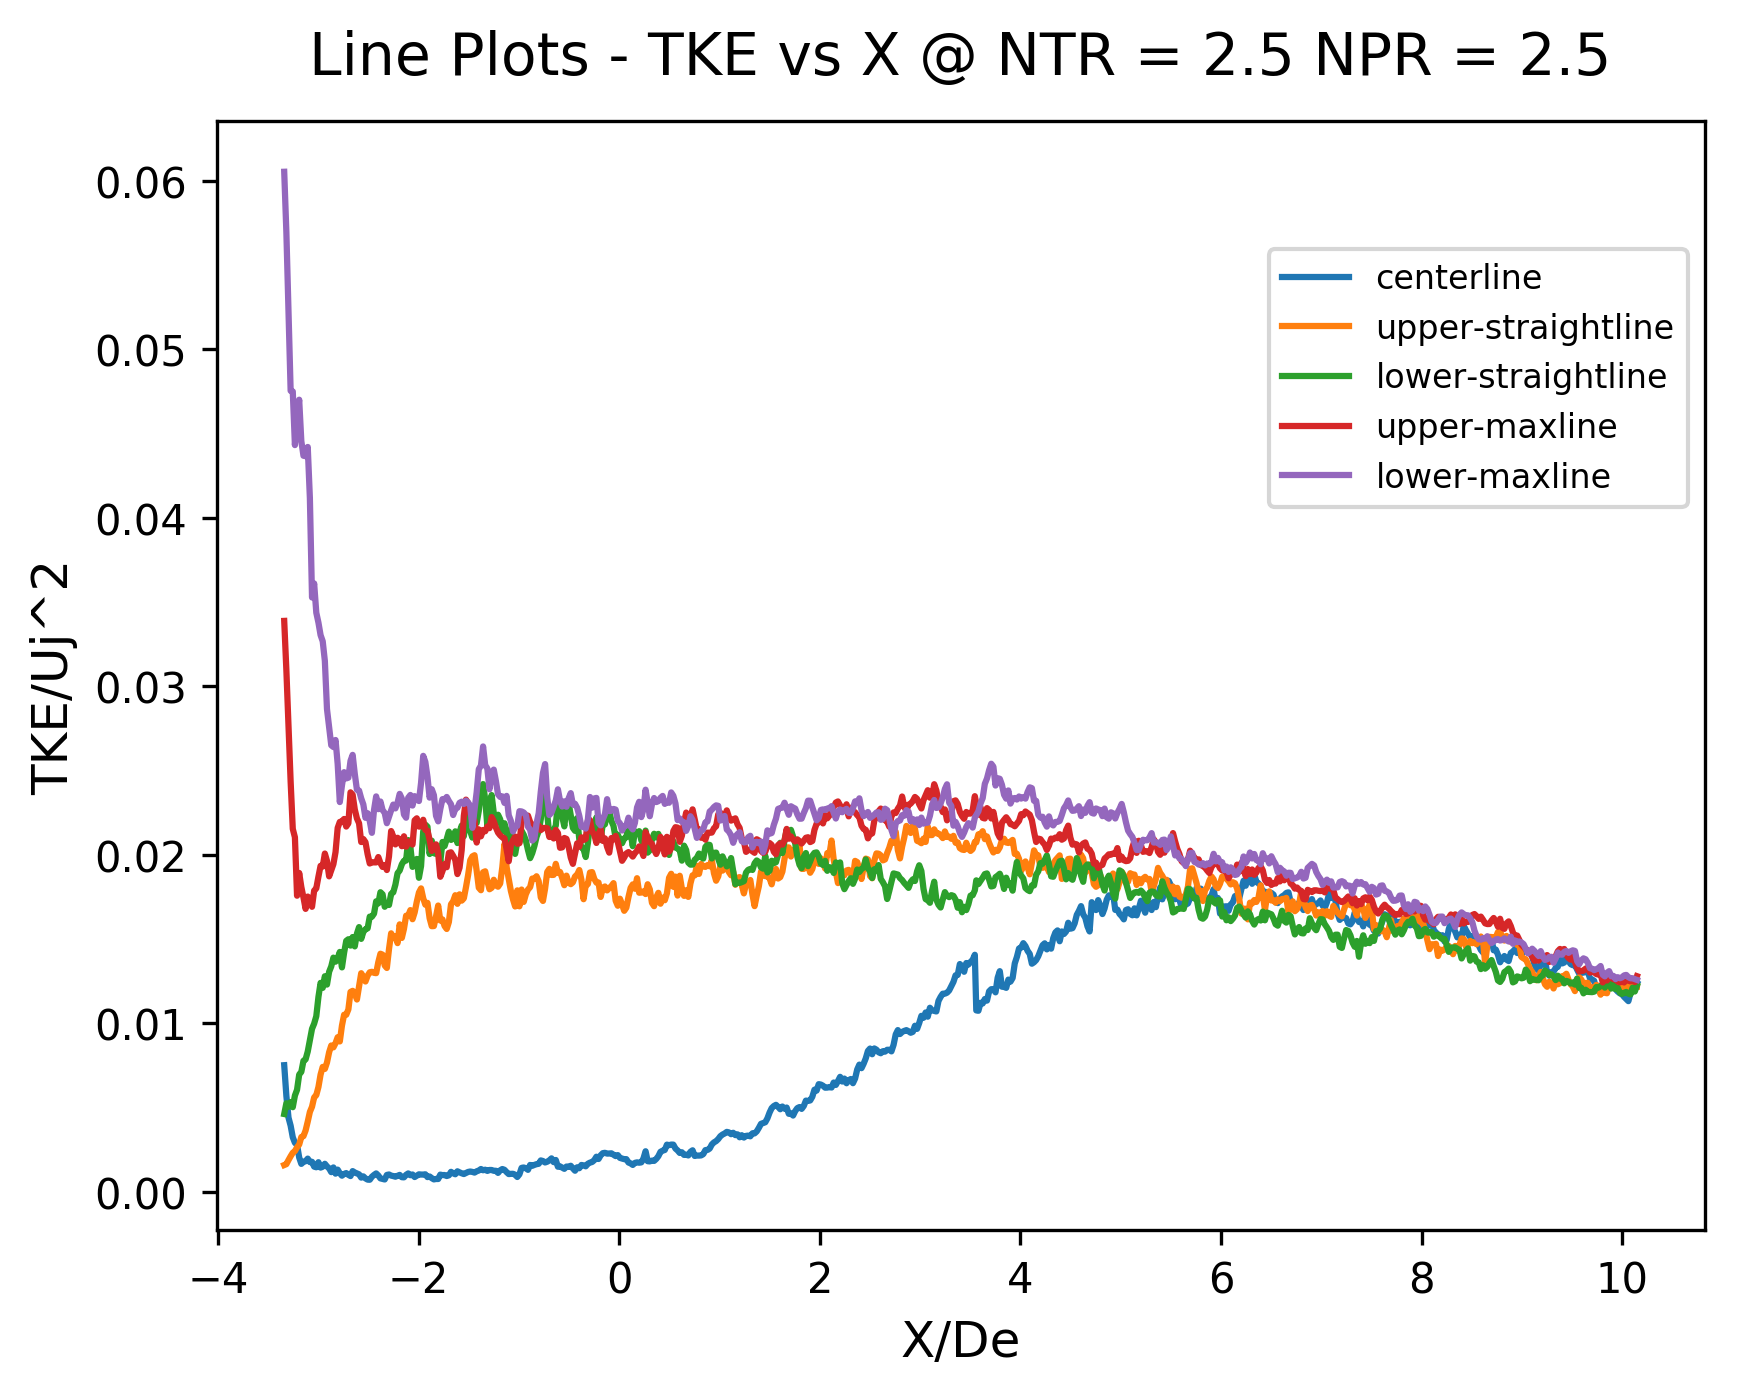
\includegraphics[width=2.5in]{images/LinePlots_TKE_NTR2p5_NPR2p5b.png}
	\caption{NTR:2p5 NPR:2p5 - 1.085in dia }
	\label{fig:lineplotsTKEb2p52p5b}
\end{subfigure}
\begin{subfigure}{.5\textwidth}
	\centering
	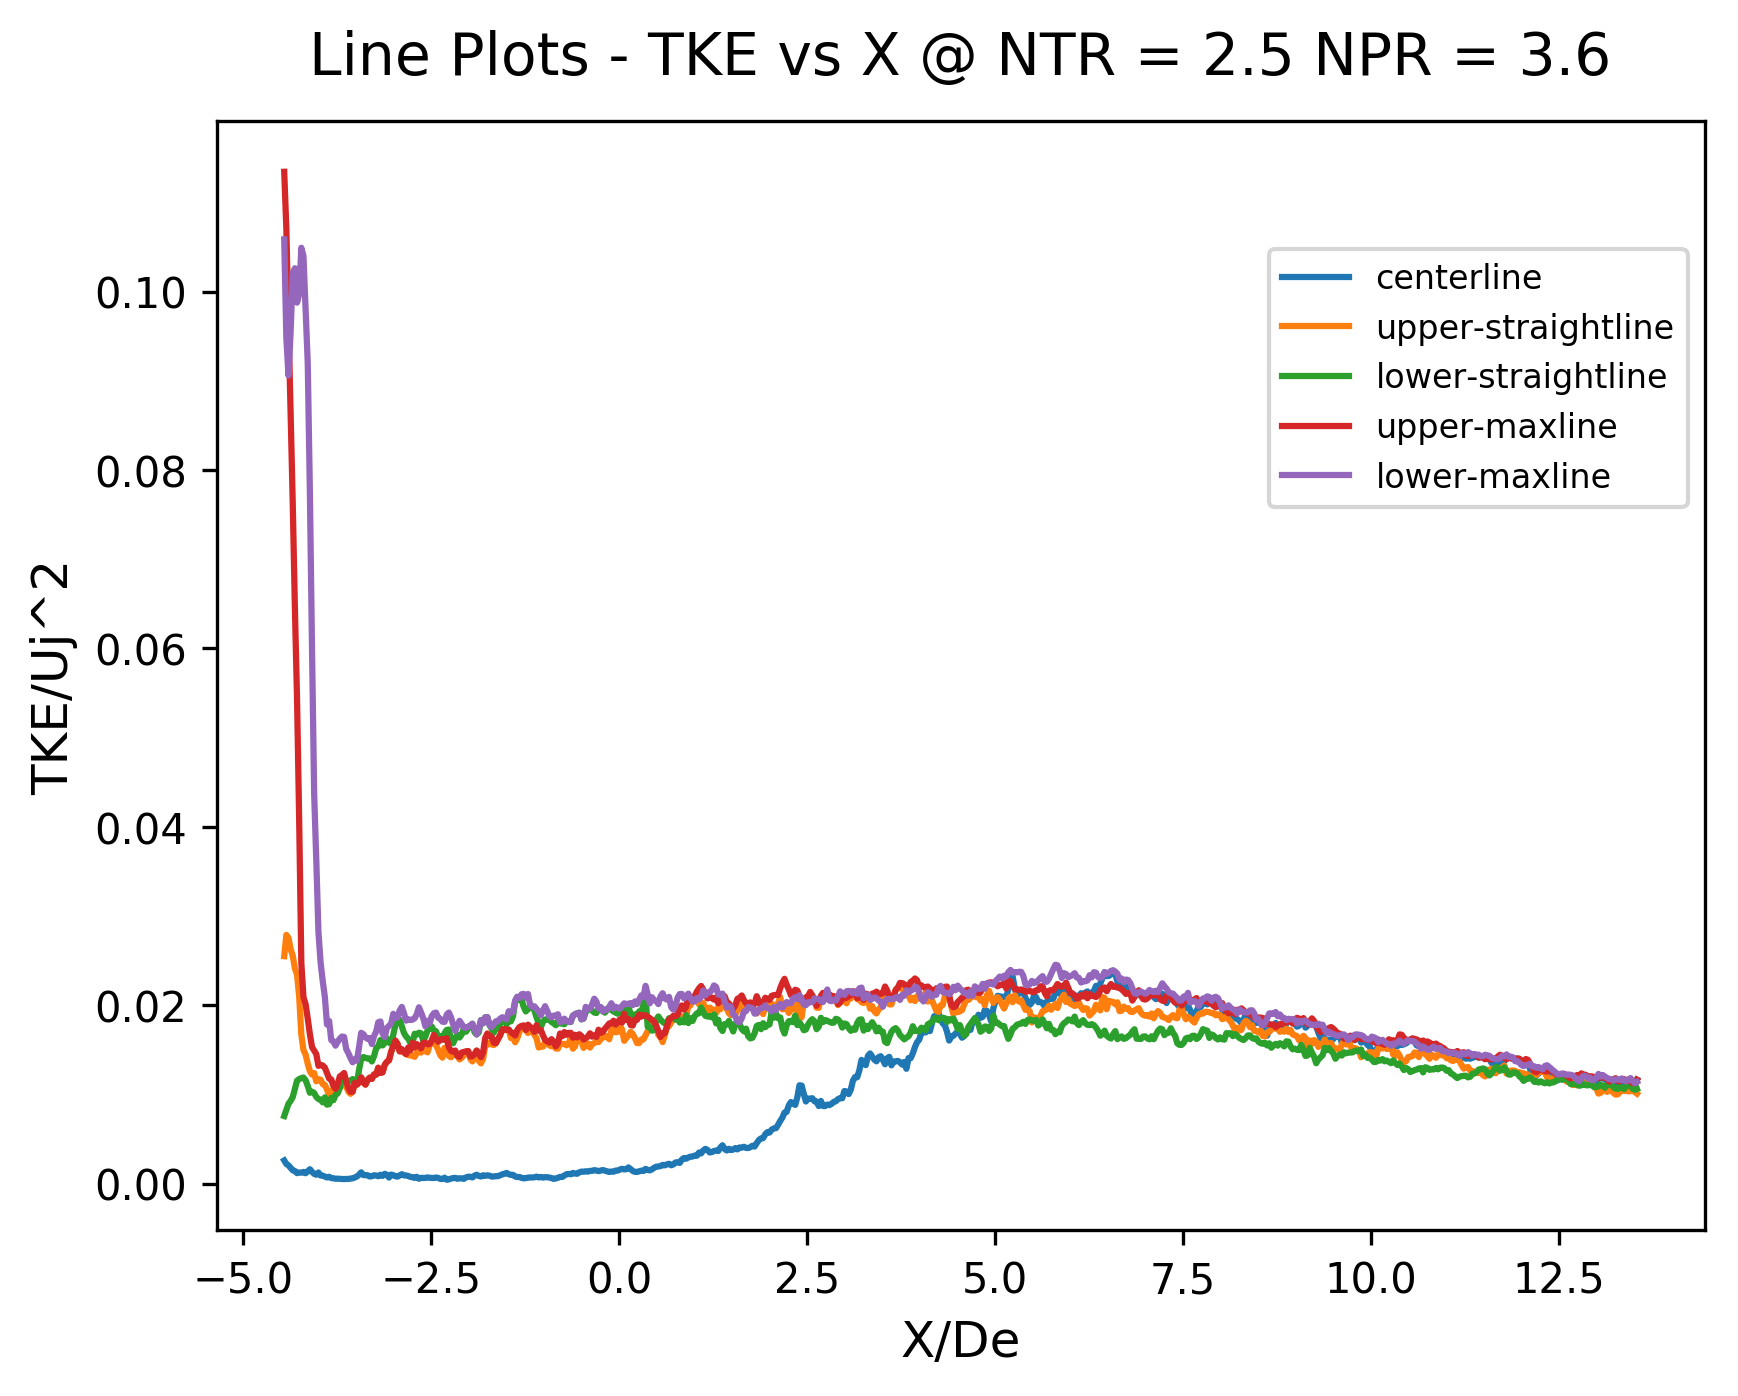
\includegraphics[width=2.5in]{images/LinePlots_TKE_NTR2p5_NPR3p6.png}
	\caption{NTR:2p5 NPR:3p6 - 0.813in dia}
	\label{fig:lineplotsTKEb2p53p6}
\end{subfigure}%
\begin{subfigure}{.5\textwidth}
	\centering
	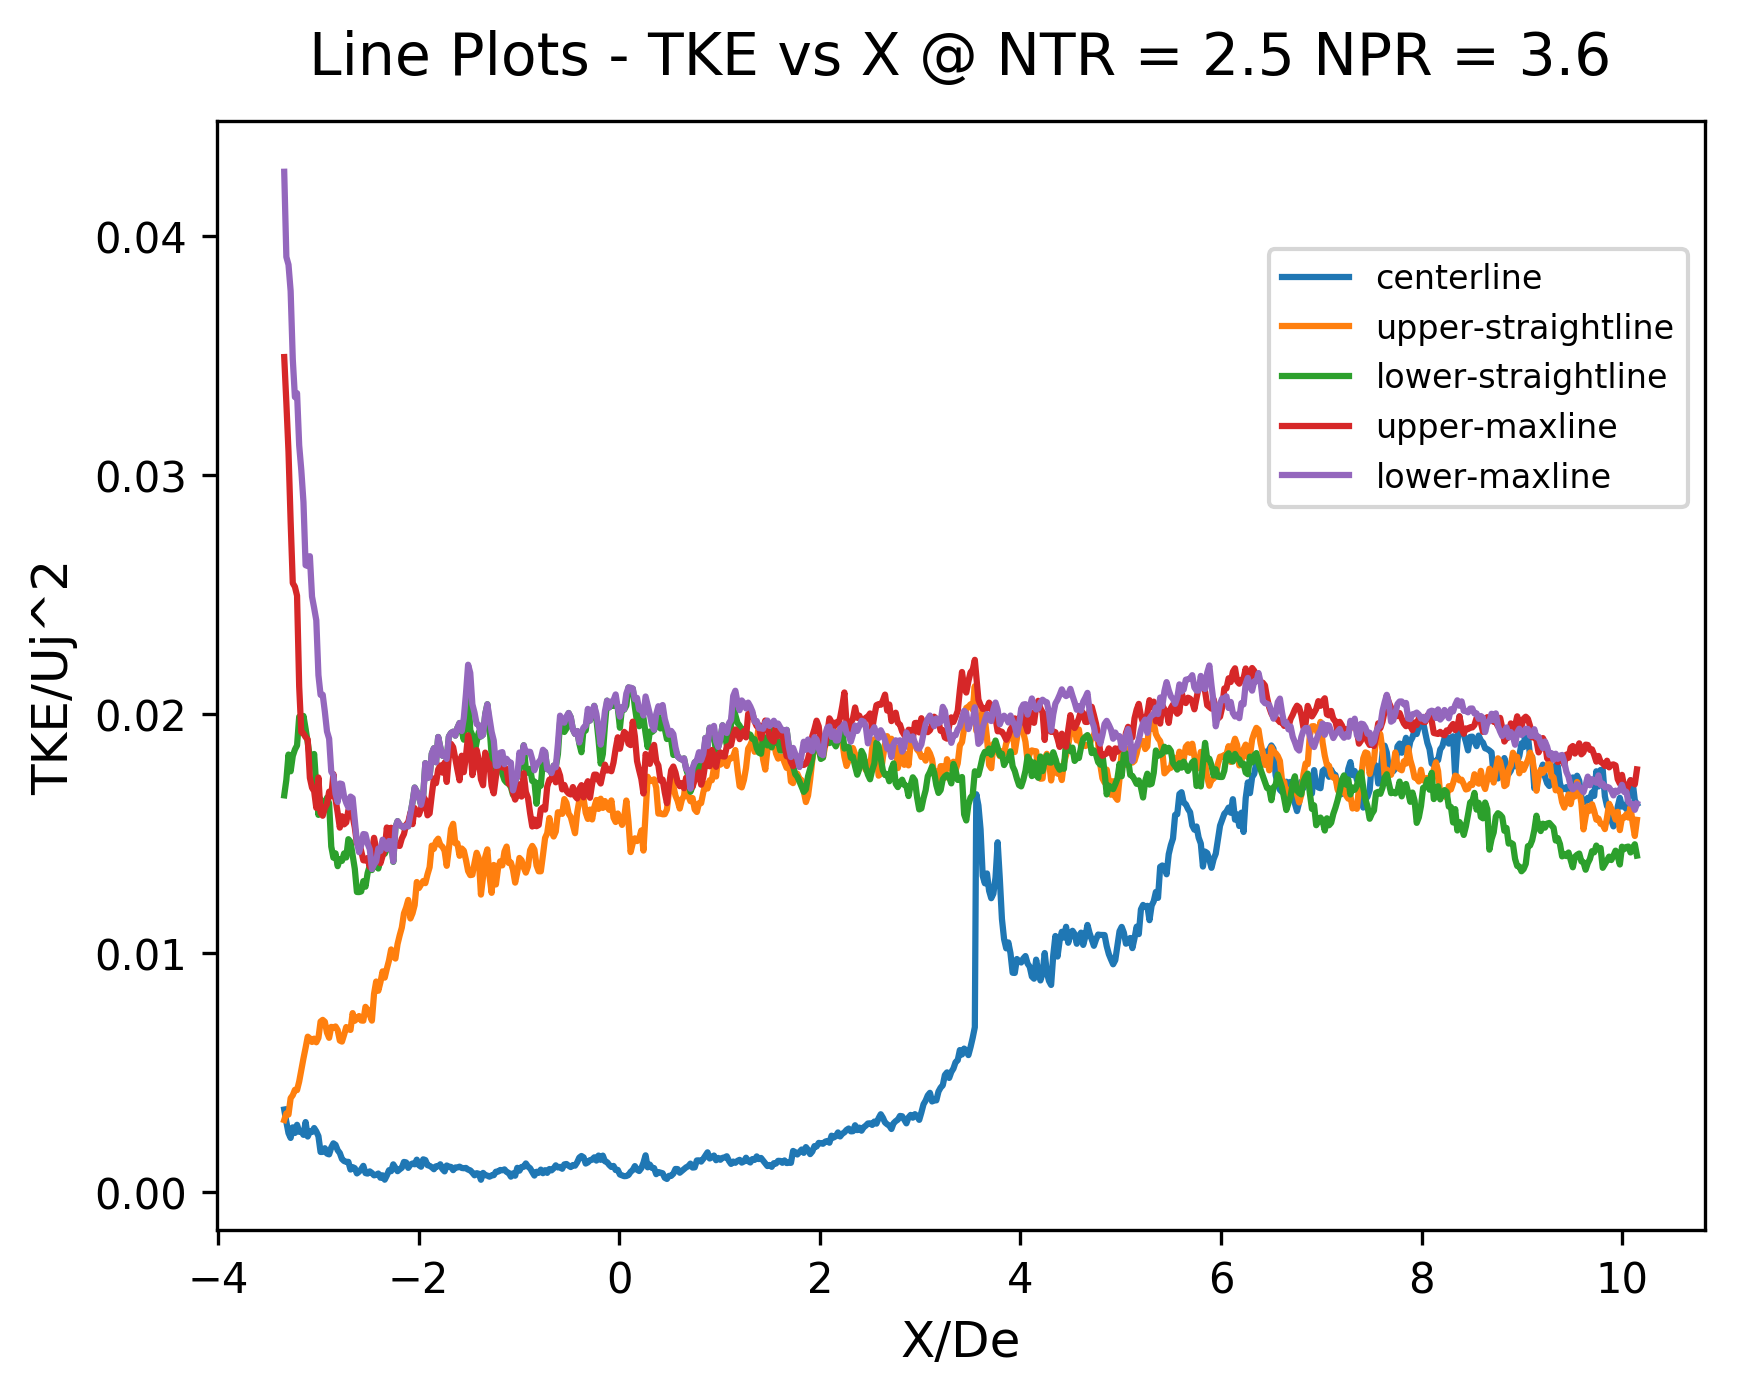
\includegraphics[width=2.5in]{images/LinePlots_TKE_NTR2p5_NPR3p6b.png}
	\caption{NTR:2p5 NPR:3p6 - 1.085in dia}
	\label{fig:lineplotsTKEb2p53p6b}
\end{subfigure}
\begin{subfigure}{.5\textwidth}
	\centering
	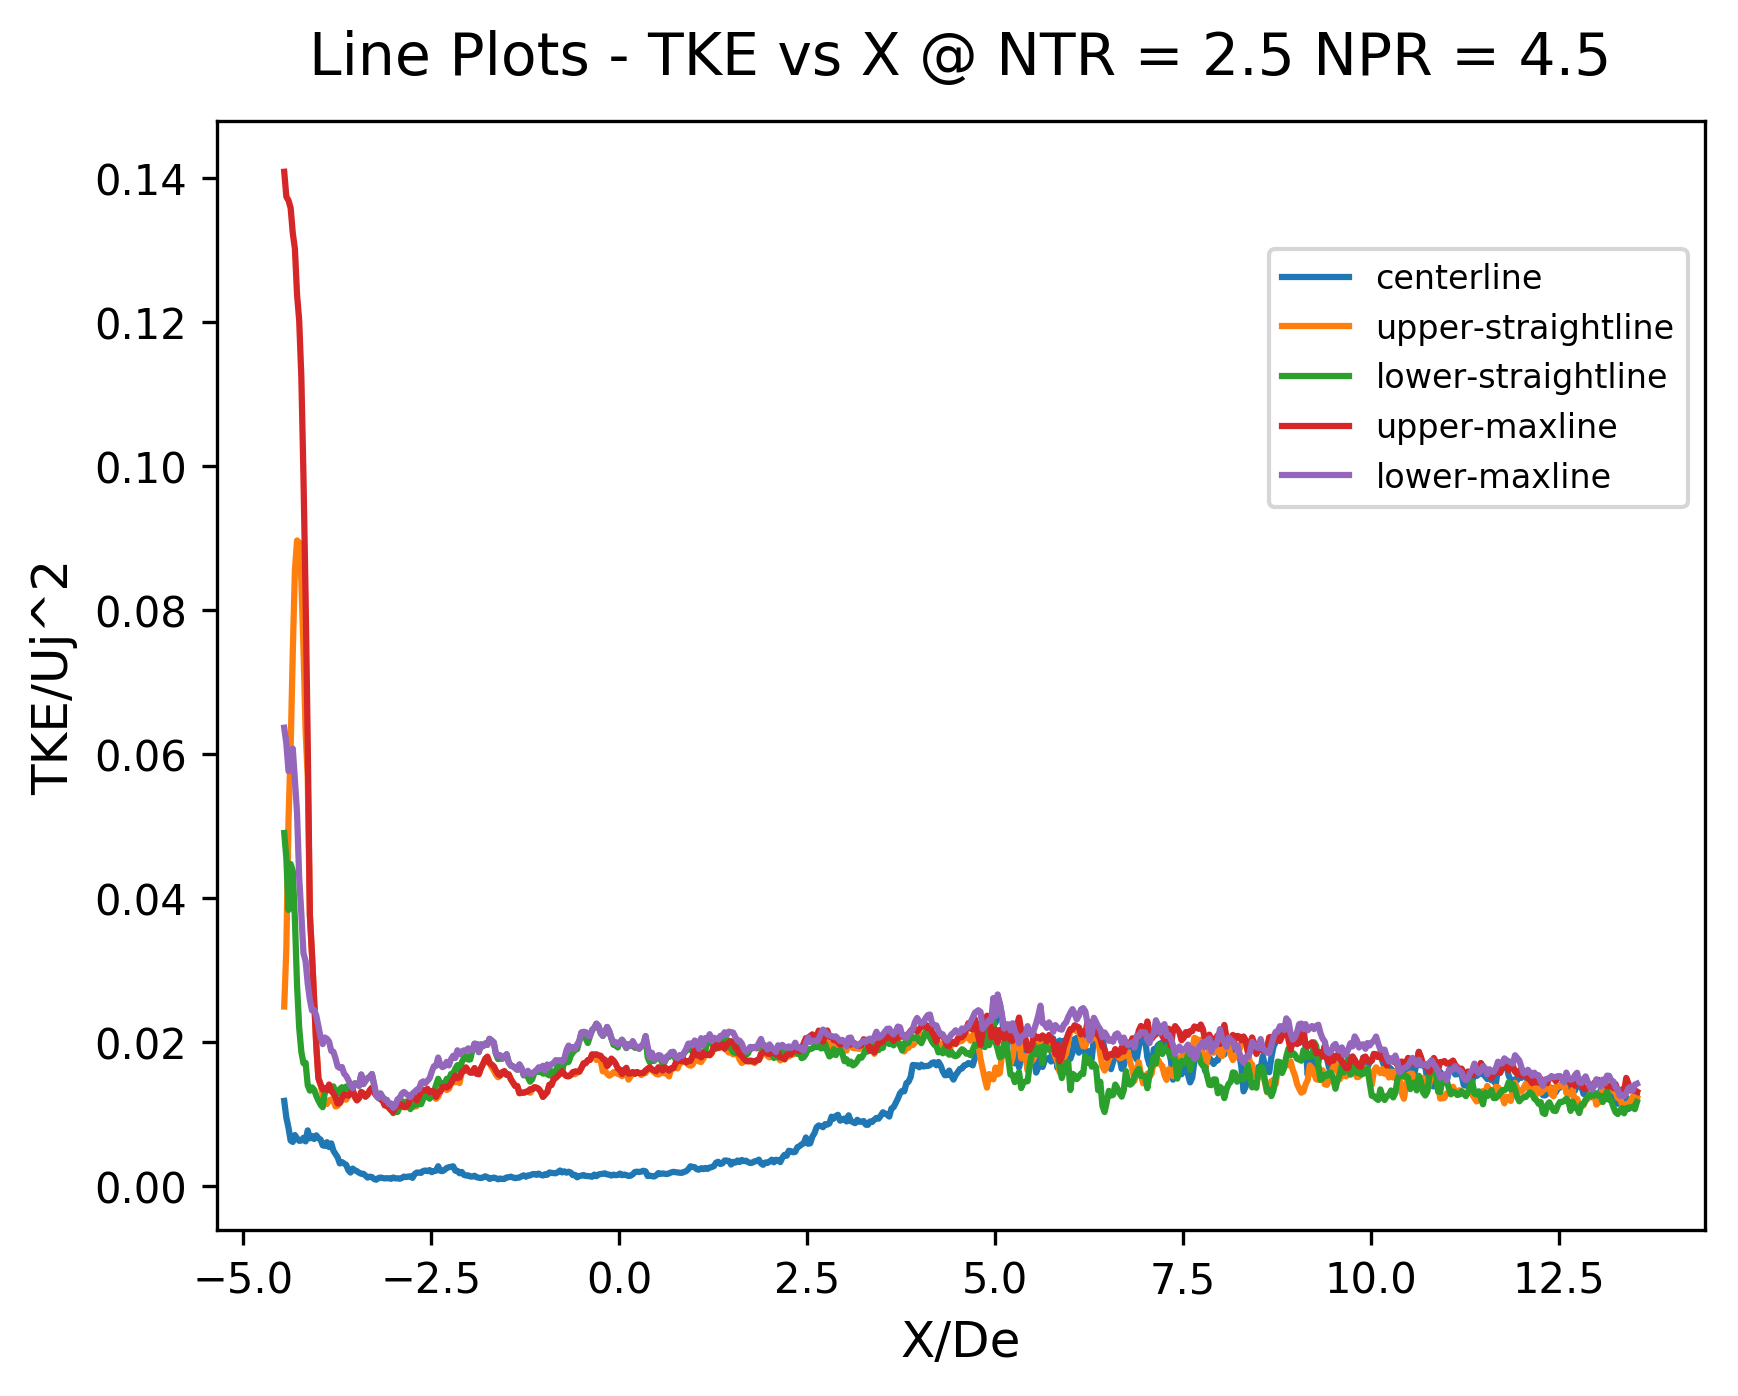
\includegraphics[width=2.5in]{images/LinePlots_TKE_NTR2p5_NPR4p5.png}
	\caption{NTR:2p5 NPR:4p5 - 0.813in dia}
	\label{fig:lineplotsTKEb2p54p5}
\end{subfigure}%
\begin{subfigure}{.5\textwidth}
	\centering
	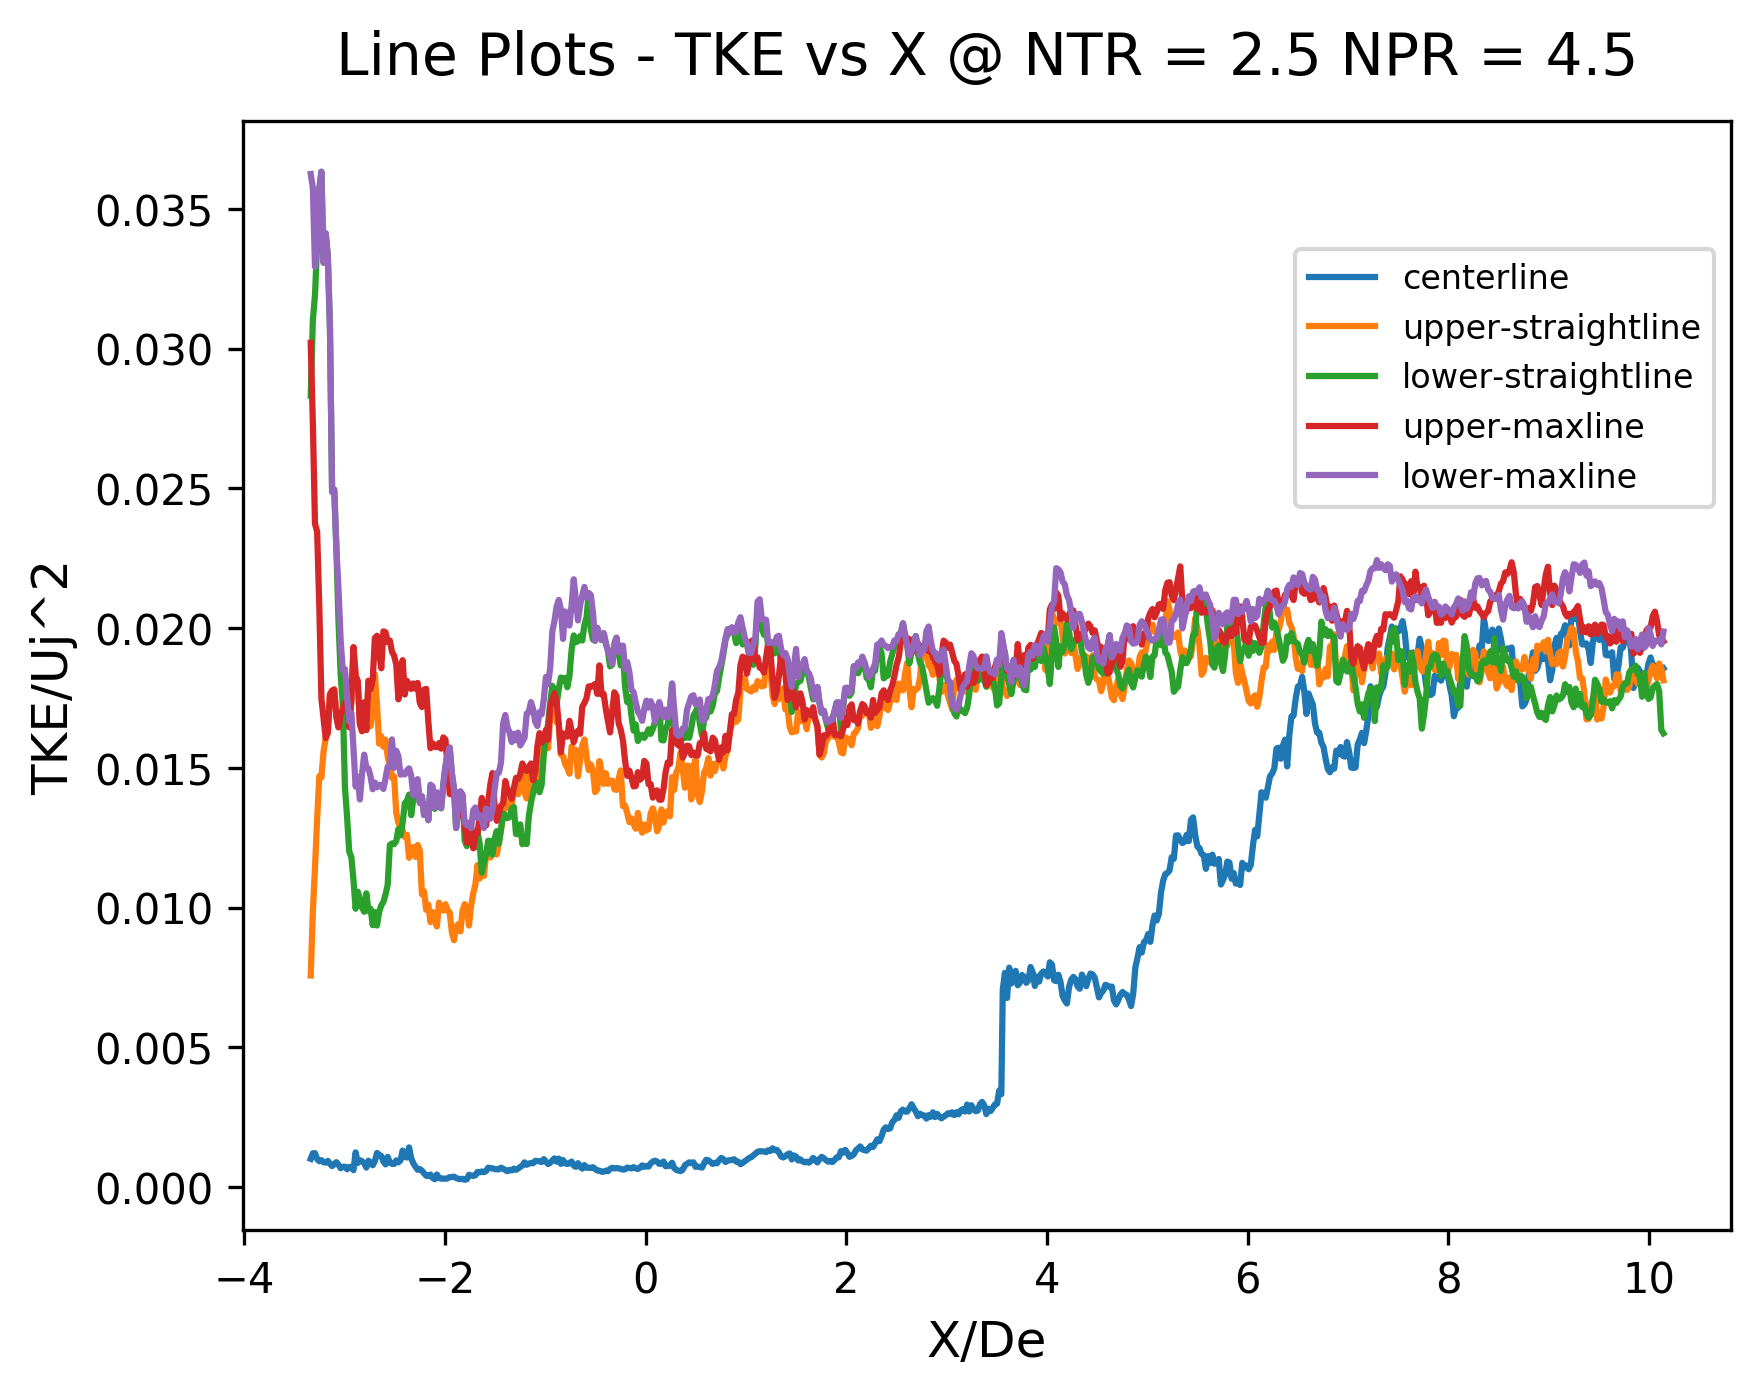
\includegraphics[width=2.5in]{images/LinePlots_TKE_NTR2p5_NPR4p5b.png}
	\caption{NTR:2p5 NPR:4p5 - 1.085in dia}
	\label{fig:lineplotsTKEb2p54p5b}
\end{subfigure}
\caption{centreline plots for TKE with dia 0.813in and 1.085in }
\label{fig:lineplotsTKEb}
\end{figure}


 
\section{Summary}

Various visualization techniques, including FFT and spectogram, have been used to gather as much information as possible from velocity, TKE of steady PIV data. Shock cell lengths observed are compared with analytical values. Effect of pressure, temperature, chevron, nozzle diameter including conflicts and agreements with published data is discussed. 

%\end{document}
%\documentclass{report}
%\usepackage{fullpage}
%%\usepackage[top=1in, bottom=1in]{geometry}
%\usepackage{amsfonts}
%%for math symbols, Ex: \mathbb{N}
%\def\Definition{what does something mean}
%\usepackage{graphicx}
%\usepackage[hidelinks]{hyperref}
%\usepackage{pdfpages}
%\usepackage{float}
%\usepackage{subcaption}
%\begin{document}


\begin{thebibliography}{}

\bibitem{lighthill}
M. J. Lighthill.  ``Jet Noise", \textit{AIAA Journal, Vol. 1, No. 7,, pp. 1507-1517}, 1963.

\bibitem{tam1}
C.K.W.Tam,\ J.M.Seiner,\ J.C.Yu,\ ``Proposed relationship between broadband shock associated noise and screech tones", \textit{Journal of Sound and Vibration 110, Issue 2, Pages 309-321}, 22 October 1986.

\bibitem{tam2}
C.K.W.Tam,\ H.K.Tanna,\ ``Shock associated noise of supersonic jets from convergent-divergent nozzles", \textit{Journal of Sound and Vibration 81, Issue 3, Pages 337-358}, 8 April 1982.

\bibitem{pablo}
Pablo A. Mora,\ Jeffrey F. Kastner,\ Ephraim J. Gutmark,\ and Kailas Kailasanath. ``Investigation of a Heated Supersonic Jet Chevrons Nozzle",\textit{53rd AIAA Aerospace Sciences Meeting, AIAA SciTech Forum}, (AIAA 2015-0233)

\bibitem{heeb}
N. Heeb,\ E. Gutmark,\ and K. Kailasanath.  ``Investigation of Chevron Penetration’s Effect on Supersonic Jet Noise Reduction", \textit{AIAA Journal, Vol. 54, No. 3 , pp. 1135-1139.}, 2016.

\bibitem{tam3}
C.K.W.Tam,\ ``Supersonic Jet Noise", \textit{Annual Review of Fluid Mechanics
Vol. 27:17-43}, Jan 1995. 

\bibitem{spectogram}
\textit{https://docs.scipy.org/doc/scipy/reference/generated/scipy.signal.spectrogram.html}, Dec 2017.

\end{thebibliography}

%\end{document}

%\usepackage{listings}

\chapter{Appendix}
%\newpage
%\appendix
%\section{Appendix:Python code}

\begin{lstlisting}[language=Python]
'''
@author: raghuvir
project: PIV Data Analysis - supersonic jet from circular nozzle
'''

import numpy as np
import matplotlib
from matplotlib import pyplot
from timeit import default_timer as timer
from matplotlib import colors
from numpy import abs
from scipy import signal
from numpy import fft

# Values to change for every setup
TRPR = np.array([[1.0,3.6]]) # temperature ratio, pressure ratio 
dia = 0.813*25.4 # converting exit diameter from inches to mm
jc = 0.00 # jet centre to adjust position of upper and lower lines

resX = 29 # resolution in x per 0.812inch, no need to change unless camera setup is changed
NTR = TRPR[0,0]; ntr  = str(int(NTR))+'p'+str(int((NTR%1)*10))# for naming output files
NPR = TRPR[0,1]; npr  = str(int(NPR))+'p'+str(int((NPR%1)*10))

print('working on NTR : '+ntr+' and NPR : '+npr)

try : 
    Vx1 = np.genfromtxt('B00001down_'+ntr+'_'+npr+'.dat',skip_header=3, invalid_raise=False)
    Vx2 = np.genfromtxt('B00001up_'+ntr+'_'+npr+'.dat',skip_header=3, invalid_raise=False)
    TKE1 = np.genfromtxt('B00004down_'+ntr+'_'+npr+'.dat',skip_header=3, invalid_raise=False)
    TKE2 = np.genfromtxt('B00004up_'+ntr+'_'+npr+'.dat',skip_header=3, invalid_raise=False)
    Vy1 = np.genfromtxt('B00002down_'+ntr+'_'+npr+'.dat',skip_header=3, invalid_raise=False)
    Vy2 = np.genfromtxt('B00002up_'+ntr+'_'+npr+'.dat',skip_header=3, invalid_raise=False)
except IOError :
    print('Please check the name format. Ex : BOOO1up_1.0_3.6 where 1.0 is ntr & 3.6 is npr')
    exit()
print(np.shape(Vx1))

# Correcting the positions of images manually before merging
Vx1[22360:,0] =  Vx1[22360:,0] + Vx1[22359,0] - Vx1[0,0] -10
Vx2[:22360,0] =  Vx2[:22360,0] + Vx1[-1,0] - Vx1[0,0] - 9
Vx2[22360:,0] =  Vx2[22360:,0] + Vx2[22359,0] - Vx1[0,0] -10
Vx1[22360:,1] =  Vx1[22360:,1] - 1
Vx2[:22360,1] =  Vx2[:22360,1] + 2.8
Vx2[22360:,1] =  Vx2[22360:,1] + 1.8   

TKE1[22360:,0] =  TKE1[22360:,0] + TKE1[22359,0] - TKE1[0,0] - 10
TKE2[:22360,0] =  TKE2[:22360,0] + TKE1[-1,0] - TKE1[0,0] - 9
TKE2[22360:,0] =  TKE2[22360:,0] + TKE2[22359,0] - TKE1[0,0] -10
TKE1[22360:,1] =  TKE1[22360:,1] - 1
TKE2[:22360,1] =  TKE2[:22360,1] + 2.8
TKE2[22360:,1] =  TKE2[22360:,1] + 1.8

Vy1[22360:,0] =  Vy1[22360:,0] + Vy1[22359,0] - Vy1[0,0] -10
Vy2[:22360,0] =  Vy2[:22360,0] + Vy1[-1,0] - Vy1[0,0] - 9
Vy2[22360:,0] =  Vy2[22360:,0] + Vy2[22359,0] - Vy1[0,0] -10
Vy1[22360:,1] =  Vy1[22360:,1] - 1
Vy2[:22360,1] =  Vy2[:22360,1] + 2.8
Vy2[22360:,1] =  Vy2[22360:,1] + 1.8

Vx = np.concatenate([Vx1,Vx2], axis=0)
TKE = np.concatenate([TKE1,TKE2])
Vy = np.concatenate([Vy1,Vy2], axis=0)

Velmax = np.max(Vx[:,2])

pyplot.figure(1)
g = pyplot.figure(figsize=(30,24))
g.clear()
subplot1 = pyplot.subplot(2,1,1)
subplot2 = pyplot.subplot(2,1,2)
matplotlib.rcParams.update({'font.size': 25})
#cm = matplotlib.cm.get_cmap('RdYlBu')

X, Y, ZVx = Vx.T; X = X/dia; Y = Y/dia; ZVx = ZVx/Velmax ; # to plot centerlines
dum = subplot1.scatter(X, Y, c = ZVx, cmap = pyplot.cm.jet,s=60); g.colorbar(dum, ax = subplot1,pad=0.015)
subplot1.set_title('Vx magnitudes, Vx/Uj', fontsize = 30, y = 1.02  )  
subplot1.set_xlabel('X-value, X/De', fontsize = 25);subplot1.set_ylabel('Y-value, Y/De', fontsize = 25)
subplot1.margins(0.003) ; subplot1.tick_params(labelsize=20)
subplot1.set_ylim([-1.5,1.5])
      
X, Y, Z = TKE.T; X = X/dia; Y = Y/dia; Z = Z/(Velmax**2.0)
dum = subplot2.scatter(X, Y, c = np.power(Z,0.5), cmap = pyplot.cm.jet,s=60); g.colorbar(dum, ax = subplot2,pad=0.015)
subplot2.set_title('TKE magnitudes (color scale normalized with square root), TKE/Uj^2', fontsize = 30, y=1.02 )  
subplot2.set_xlabel('X-value, X/De', fontsize = 25);subplot2.set_ylabel('Y-value, Y/De', fontsize = 25)
subplot2.margins(0.003) ; subplot2.tick_params(labelsize=20); subplot2.set_ylim([-1.5,1.5])
g.suptitle('PIV data at NTR = '+str(NTR)+' and NPR = '+str(NPR), fontsize = 40, x = 0.47, y =0.95)
pyplot.savefig('PIV_'+'NTR'+str(NTR)+'_NPR'+str(NPR)+'.png',bbox_inches = 'tight', pad_inches = 0.4)

pyplot.figure(2); pyplot.clf()
matplotlib.rcParams.update({'font.size': 6})
X, Y, ZVy = Vy.T; X = X/dia; Y = Y/dia; ZVy = ZVy/(Velmax); ax1 = pyplot.gca();
dum = pyplot.scatter(X, Y, c = np.power(ZVy,1), cmap = pyplot.cm.jet,s=60); pyplot.colorbar(dum, ax = ax1,pad=0.015)
#pyplot.title('Vy magnitudes, Vy/Uj', fontsize = 15, y=1.02 )  
pyplot.xlabel('X-value, X/De', fontsize = 8);pyplot.ylabel('Y-value, Y/De', fontsize = 8)
pyplot.margins(0.003) ; subplot2.tick_params(labelsize=6); pyplot.ylim([-1.5,1.5])
pyplot.title('Vy - PIV data at NTR = '+str(NTR)+' and NPR = '+str(NPR), fontsize = 10, x = 0.51, y =1.01)
gcf1 = pyplot.gcf(); gcf1.set_size_inches(8,3)
pyplot.savefig('PIV_Vy_'+'NTR'+str(NTR)+'_NPR'+str(NPR)+'.png',dpi=300,bbox_inches = 'tight')

#centerline
dummyc = (abs(jc-Y)==np.min(abs(jc-Y[0:22360]))) | (abs(jc-Y)==np.min(abs(jc-Y[22360:44720]))) | (abs(jc-Y)==np.min(abs(jc-Y[44720:67080]))) | (abs(jc-Y)==np.min(abs(jc-Y[67080:89438])))
dummyc = dummyc & (Z>0.0001) #ignoring data with z value as 0

#xlines is xvalues, zlines is tke values, vlines is velocity values
Xlinesc = X[dummyc]; Zlinesc = Z[dummyc]; Vlinesc = ZVx[dummyc];Vylinesc = ZVy[dummyc]
#correcting for smooth transition between images when merged
for j in np.arange(Xlinesc.shape[0]-1):
    if Xlinesc[j+1] < Xlinesc[j] :
        Xlinesc[j+1] = Xlinesc[j]
        Zlinesc[j+1] = Zlinesc[j]
        Vlinesc[j+1] = Vlinesc[j]
        Vylinesc[j+1] = Vylinesc[j]

#upper line
dummyu = (abs(0.5+jc-Y)==np.min(abs(0.5+jc-Y[0:22360]))) | (abs(0.5+jc-Y)==np.min(abs(0.5+jc-Y[22360:44720]))) | (abs(0.5+jc-Y)==np.min(abs(0.5+jc-Y[44720:67080]))) | (abs(0.5+jc-Y)==np.min(abs(0.5+jc-Y[67080:89438])))
dummyu = dummyu & (Z>0.0001) #ignoring data with z value as 0

Xlinesu = X[dummyu]; Zlinesu = Z[dummyu];Vlinesu = ZVx[dummyu];Vylinesu = ZVy[dummyu]
#correcting for smooth transition between images when merged

for j in np.arange(Xlinesu.shape[0]-1):
    if Xlinesu[j+1] < Xlinesu[j] :
        Xlinesu[j+1] = Xlinesu[j]
        Zlinesu[j+1] = Zlinesu[j]
        Vlinesu[j+1] = Vlinesu[j]
        Vylinesu[j+1] = Vylinesu[j]
     
#lower line
dummyl = (abs(jc-0.5-Y)==np.min(abs(jc-0.5-Y[0:22360]))) | (abs(jc-0.5-Y)==np.min(abs(jc-0.5-Y[22360:44720]))) | (abs(jc-0.5-Y)==np.min(abs(jc-0.5-Y[44720:67080]))) | (abs(jc-0.5-Y)==np.min(abs(jc-0.5-Y[67080:89438])))
dummyl = dummyl & (Z>0.0001) #ignoring data with z value as 0

Xlinesl = X[dummyl]; Zlinesl = Z[dummyl];Vlinesl = ZVx[dummyl];Vylinesl = ZVy[dummyl]
#correcting for smooth transition between images when merged
for j in np.arange(Xlinesl.shape[0]-1):
    if Xlinesl[j+1] < Xlinesl[j] :
        Xlinesl[j+1] = Xlinesl[j]
        Zlinesl[j+1] = Zlinesl[j]  
        Vlinesl[j+1] = Vlinesl[j]
        Vylinesl[j+1] = Vylinesl[j]

#upper max
Z1 = Z[0:22360].reshape(130,172);         X1 = X[0:22360].reshape(130,172);
Z2 = Z[22360:44720].reshape(130,172) ;    X2 = X[22360:44720].reshape(130,172) ;
Z3 = Z[44720:67080].reshape(130,172);     X3 = X[44720:67080].reshape(130,172); 
Z4 = Z[67080:89440].reshape(130,172) ;    X4 = X[67080:89440].reshape(130,172) ;
ZVx1 = ZVx[0:22360].reshape(130,172);         
ZVx2 = ZVx[22360:44720].reshape(130,172) ;    
ZVx3 = ZVx[44720:67080].reshape(130,172);     
ZVx4 = ZVx[67080:89440].reshape(130,172) ;   
  
Zcomplete = np.concatenate((Z1,Z2,Z3,Z4),axis=1); ZVxcomplete = np.concatenate((ZVx1,ZVx2,ZVx3,ZVx4),axis=1)
Xcomplete = np.concatenate((X1,X2,X3,X4),axis=1)
[Zcompleteu, Zcompletel] = np.vsplit(Zcomplete,2) ;[ZVxcompleteu, ZVxcompletel] = np.vsplit(ZVxcomplete,2)
[Xcompleteu, Xcompletel] = np.vsplit(Xcomplete,2)
Zmaxu = np.amax(Zcompleteu,axis=0);Zmaxl = np.amax(Zcompletel,axis=0)
ZVxmaxu = np.amax(ZVxcompleteu,axis=0);ZVxmaxl = np.amax(ZVxcompletel,axis=0)
Xmaxu = np.amax(Xcompleteu,axis=0);Xmaxl = np.amax(Xcompletel,axis=0)

for j in np.arange(Xmaxu.shape[0]-1):
    if Xmaxu[j+1] < Xmaxu[j] :
        Xmaxu[j+1] = Xmaxu[j]
        Zmaxu[j+1] = Zmaxu[j] 
        ZVxmaxu[j+1] = ZVxmaxu[j] 

Xmaxu_TKE = Xmaxu[Zmaxu>0.0001];Zmaxu = Zmaxu[Zmaxu>0.0001];
Xmaxu_Vx = Xmaxu[ZVxmaxu>0.0001];ZVxmaxu = ZVxmaxu[ZVxmaxu>0.0001]

for j in np.arange(Xmaxl.shape[0]-1):
    if Xmaxl[j+1] < Xmaxl[j] :
        Xmaxl[j+1] = Xmaxl[j]
        Zmaxl[j+1] = Zmaxl[j] 
        ZVxmaxl[j+1] = ZVxmaxl[j] 
        
Xmaxl_TKE = Xmaxl[Zmaxl>0.0001];Zmaxl = Zmaxl[Zmaxl>0.0001];
Xmaxl_Vx = Xmaxl[ZVxmaxl>0.0001];ZVxmaxl = ZVxmaxl[ZVxmaxl>0.0001]

pyplot.figure(3);
pyplot.plot(Xlinesc,Zlinesc,label="centerline") 
pyplot.plot(Xlinesu,Zlinesu,label="upper-straightline") 
pyplot.plot(Xlinesl,Zlinesl,label="lower-straightline") 
pyplot.plot(Xmaxu_TKE,Zmaxu,label="upper-maxline")
pyplot.plot(Xmaxl_TKE,Zmaxl,label="lower-maxline")
matplotlib.rcParams.update({'font.size': 10})
pyplot.legend( bbox_to_anchor=(1, 0.9), fontsize =8); 
pyplot.tick_params(labelsize=10)
pyplot.xlabel('X/De',fontsize=12); pyplot.ylabel('TKE/Uj^2',fontsize=12)    
pyplot.title('Line Plots - TKE vs X @ NTR = '+str(NTR)+' NPR = '+str(NPR), y = 1.02,fontsize=14)
pyplot.savefig('LinePlots_TKE_'+'NTR'+str(NTR)+'_NPR'+str(NPR)+'.png',bbox_inches='tight',  dpi=300)

pyplot.figure(4);
pyplot.plot(Xlinesc,Vlinesc,label="centerline")
pyplot.plot(Xlinesu,Vlinesu,label="upper-straightline")  
pyplot.plot(Xlinesl,Vlinesl,label="lower-straightline")  
pyplot.plot(Xmaxu_Vx,ZVxmaxu,label="upper-maxline")
pyplot.plot(Xmaxl_Vx,ZVxmaxl,label="lower-maxline")   
matplotlib.rcParams.update({'font.size': 10})
pyplot.legend( bbox_to_anchor=(1, 0.9), fontsize =8); 
pyplot.tick_params(labelsize=10)
pyplot.xlabel('X/De', fontsize=12); pyplot.ylabel('Vx/Uj', fontsize=12)    
pyplot.title('Line Plots - Vx vs X @ NTR = '+str(NTR)+' NPR = '+str(NPR), y = 1.02, fontsize=14)
pyplot.savefig('LinePlots_Vx_'+'NTR'+str(NTR)+'_NPR'+str(NPR)+'.png', bbox_inches='tight', dpi=300)
   
pyplot.figure(5);
pyplot.plot(Xlinesc,Vylinesc,label="centerline")
pyplot.plot(Xlinesu,Vylinesu,label="upper-straightline")  
pyplot.plot(Xlinesu,Vylinesl,label="lower-straightline")  
matplotlib.rcParams.update({'font.size': 10})
pyplot.legend( bbox_to_anchor=(1, 0.9), fontsize =8); 
pyplot.tick_params(labelsize=10)
pyplot.xlabel('X/De', fontsize=12); pyplot.ylabel('Vy/Uj', fontsize=12)    
pyplot.title('Line Plots - Vy vs X @ NTR = '+str(NTR)+' NPR = '+str(NPR), y = 1.02, fontsize=14)
pyplot.savefig('LinePlots_Vy_'+'NTR'+str(NTR)+'_NPR'+str(NPR)+'.png', bbox_inches='tight', dpi=300)
   
#---------------FFT--Vx--------------------------------------------

pyplot.figure(6)
matplotlib.rcParams.update({'font.size': 10})
Hxc = abs(fft.fft(Vlinesc));Hxu = abs(fft.fft(Vlinesu));Hxl = abs(fft.fft(Vlinesl));
Hx2c = Hxc[4:np.size(Vlinesc)/2]; Hx2u = Hxu[4:np.size(Vlinesu)/2]; Hx2l = Hxl[4:np.size(Vlinesl)/2]; 
freqXc = fft.fftfreq(len(Vlinesc), 1/resX);freqX2c = 1/freqXc[4:np.size(Vlinesc)/2] 
freqXu = fft.fftfreq(len(Vlinesu), 1/resX);freqX2u = 1/freqXu[4:np.size(Vlinesu)/2]
freqXl = fft.fftfreq(len(Vlinesl), 1/resX);freqX2l = 1/freqXl[4:np.size(Vlinesl)/2]

pyplot.plot(freqX2c*0.813*25.4/dia, Hx2c, label='Vx_centerline') #divide by 0.813 since sampling rate is adjusted to that dia i.e., 1/resX of 0.813
pyplot.plot(freqX2u*0.813*25.4/dia, Hx2u, label='Vx_upperline')
pyplot.plot(freqX2l*0.813*25.4/dia, Hx2l, label='Vx_lowerline')

pyplot.tight_layout(); pyplot.legend(fontsize =8);
pyplot.tick_params(labelsize=10);pyplot.xticks(np.arange(0,6,0.5));
axes = pyplot.gca();  #axes.xaxis.grid(True, which='major');axes.xaxis.grid(False, which='minor');#pyplot.minorticks_on()
pyplot.ylabel(' PSD (FFT) ', fontsize=12);pyplot.xlabel('Wavelength(/De)', fontsize=12)
pyplot.title('Wavelength spectrum of Vx'+' at NTR '+str(NTR)+', NPR '+str(NPR), fontsize=15, y=1.01)
pyplot.savefig('Fft_Vx_'+'NTR'+str(NTR)+'_NPR'+str(NPR)+'.png', dpi=300, bbox_inches='tight')

#---------------Vx SPECTOGRAM------------

freqs_1,times_1, spec_1 = signal.spectrogram(ZVxmaxu,resX,window='hanning', nperseg=np.size(ZVxmaxu)/6, noverlap=np.size(ZVxmaxu)/6.04,detrend=False,scaling='spectrum');
freqs_2,times_2, spec_2 = signal.spectrogram(Vlinesu,resX,window='hanning', nperseg=np.size(Vlinesu)/6.00, noverlap=np.size(Vlinesu)/6.04,detrend=False, scaling='spectrum');
freqs_3,times_3, spec_3 = signal.spectrogram(Vlinesc,resX,window='hanning', nperseg=np.size(Vlinesc)/6.00, noverlap=np.size(Vlinesc)/6.04,detrend=False, scaling='spectrum');
freqs_4,times_4, spec_4 = signal.spectrogram(ZVxmaxu,resX,window='hanning', nperseg=np.size(ZVxmaxu)/2.00, noverlap=np.size(ZVxmaxu)/2.01,detrend=False, scaling='spectrum');
freqs_5,times_5, spec_5 = signal.spectrogram(Vlinesu,resX,window='hanning', nperseg=np.size(Vlinesu)/2.00, noverlap=np.size(Vlinesu)/2.01,detrend=False, scaling='spectrum');
freqs_6,times_6, spec_6 = signal.spectrogram(Vlinesc,resX,window='hanning', nperseg=np.size(Vlinesc)/2.00, noverlap=np.size(Vlinesc)/2.01,detrend=False, scaling='spectrum');

pyplot.figure(7); matplotlib.rcParams.update({'font.size': 12})
fig = pyplot.figure(figsize=(18,9)); fig.clear()

ax1  = fig.add_subplot(231)
pcm1  = ax1.pcolormesh(times_1,freqs_1,np.log10(spec_1),cmap='jet')
fig.colorbar(pcm1,ax=ax1)
ax1.set_title('Vx - uppermax line', fontsize = 20 )  
ax1.set_xlabel('Distance from jet exit, X/De', fontsize = 15);ax1.set_ylabel('wavenumbers*De', fontsize = 15)

ax2 = fig.add_subplot(232)
pcm2  = ax2.pcolormesh(times_2,freqs_2,np.log10(spec_2),cmap='jet')
fig.colorbar(pcm2,ax=ax2)
ax2.set_title('Vx - upperstraight line', fontsize = 20 )  
ax2.set_xlabel('Distance from jet exit, X/De', fontsize = 15);ax2.set_ylabel('wavenumbers*De', fontsize = 15)

ax3  = fig.add_subplot(233)
pcm3  = ax3.pcolormesh(times_3,freqs_3,np.log10(spec_3),cmap='jet')
fig.colorbar(pcm3,ax=ax3)
ax3.set_title('Vx - center line', fontsize = 20 )  
ax3.set_xlabel('Distance from jet exit, X/De', fontsize = 15);ax3.set_ylabel('wavenumbers*De', fontsize = 15)

ax4  = fig.add_subplot(234)
pcm4  = ax4.pcolormesh(times_4,freqs_4,np.log10(spec_4),cmap='jet')
fig.colorbar(pcm4,ax=ax4)
ax4.set_title('Vx - uppermax line - HighRes', fontsize = 20 )  
ax4.set_xlabel('Distance from jet exit, X/De', fontsize = 15);ax4.set_ylabel('wavenumbers*De', fontsize = 15)

ax5  = fig.add_subplot(235)
pcm5  = ax5.pcolormesh(times_5,freqs_5,np.log10(spec_5),cmap='jet')
fig.colorbar(pcm5,ax=ax5)
ax5.set_title('Vx - upperstraight line - HighRes', fontsize = 20 )  
ax5.set_xlabel('Distance from jet exit, X/De', fontsize = 15);ax5.set_ylabel('wavenumbers*De', fontsize = 15)

ax6  = fig.add_subplot(236)
pcm6  = ax6.pcolormesh(times_6,freqs_6,np.log10(spec_6),cmap='jet')
fig.colorbar(pcm6,ax=ax6)
ax6.set_title('Vx - center line - High Res', fontsize = 20 )  
ax6.set_xlabel('Distance from jet exit, X/De', fontsize = 15);ax6.set_ylabel('wavenumbers*De', fontsize = 15)

#pyplot.xticks(fontsize=10);#pyplot.xticks(np.arange(0,6,0.5));
pyplot.suptitle('Spectogram of Vx for various lines along jet (logscaled)'+' at NTR '+str(NTR)+', NPR '+str(NPR), fontsize =25 )
pyplot.tight_layout(); fig.subplots_adjust(top=0.88)
pyplot.savefig('Spectogram_Vx_'+'NTR'+str(NTR)+'_NPR'+str(NPR)+'.png', dpi=300)

#---------------TKE SPECTOGRAM------------
freqs_upmax,times_upmax, spec_upmax = signal.spectrogram(Zmaxu,resX,window='hanning', nperseg=np.size(Zmaxu)/6, noverlap=np.size(Zmaxu)/6.04,detrend=False,scaling='spectrum');
freqs_lowmax,times_lowmax, spec_lowmax = signal.spectrogram(Zmaxl,resX,window='hanning', nperseg=np.size(Zmaxl)/6.00, noverlap=np.size(Zmaxl)/6.04,detrend=False, scaling='spectrum');
freqs_centre,times_centre, spec_centre = signal.spectrogram(Zlinesc,resX,window='hanning', nperseg=np.size(Zlinesc)/6.00, noverlap=np.size(Zlinesc)/6.04,detrend=False, scaling='spectrum');
freqs_upmaxHR,times_upmaxHR, spec_upmaxHR = signal.spectrogram(Zmaxu,resX,window='hanning', nperseg=np.size(Zmaxu)/2.00, noverlap=np.size(Zmaxu)/2.01,detrend=False, scaling='spectrum');
freqs_lowmaxHR,times_lowmaxHR, spec_lowmaxHR = signal.spectrogram(Zmaxl,resX,window='hanning', nperseg=np.size(Zmaxl)/2.00, noverlap=np.size(Zmaxl)/2.01,detrend=False, scaling='spectrum');
freqs_centreHR,times_centreHR, spec_centreHR = signal.spectrogram(Zlinesc,resX,window='hanning', nperseg=np.size(Zlinesc)/2.00, noverlap=np.size(Zlinesc)/2.01,detrend=False, scaling='spectrum');

pyplot.figure(8); matplotlib.rcParams.update({'font.size': 12})
fig = pyplot.figure(figsize=(18,9)); fig.clear()

ax1  = fig.add_subplot(231)
pcm1  = ax1.pcolormesh(times_upmax,freqs_upmax,np.log10(spec_upmax),cmap='jet')
fig.colorbar(pcm1,ax=ax1)
ax1.set_title('TKE - uppermax line', fontsize = 20 )  
ax1.set_xlabel('Distance from jet exit, X/De', fontsize = 15);ax1.set_ylabel('wavenumbers*De', fontsize = 15)

ax2 = fig.add_subplot(232)
pcm2  = ax2.pcolormesh(times_lowmax,freqs_lowmax,np.log10(spec_lowmax),cmap='jet')
fig.colorbar(pcm2,ax=ax2)
ax2.set_title('TKE - lowermax line', fontsize = 20 )  
ax2.set_xlabel('Distance from jet exit, X/De', fontsize = 15);ax2.set_ylabel('wavenumbers*De', fontsize = 15)

ax3  = fig.add_subplot(233)
pcm3  = ax3.pcolormesh(times_centre,freqs_centre,np.log10(spec_centre),cmap='jet')
fig.colorbar(pcm3,ax=ax3)
ax3.set_title('TKE - center line', fontsize = 20 )  
ax3.set_xlabel('Distance from jet exit, X/De', fontsize = 15);ax3.set_ylabel('wavenumbers*De', fontsize = 15)

ax4  = fig.add_subplot(234)
pcm4  = ax4.pcolormesh(times_upmaxHR,freqs_upmaxHR,np.log10(spec_upmaxHR),cmap='jet')
fig.colorbar(pcm4,ax=ax4)
ax4.set_title('TKE - uppermax line - HighRes', fontsize = 20 )  
ax4.set_xlabel('Distance from jet exit, X/De', fontsize = 15);ax4.set_ylabel('wavenumbers*De', fontsize = 15)

ax5  = fig.add_subplot(235)
pcm5  = ax5.pcolormesh(times_lowmaxHR,freqs_lowmaxHR,np.log10(spec_lowmaxHR),cmap='jet')
fig.colorbar(pcm5,ax=ax5)
ax5.set_title('TKE - lowermax line - HighRes', fontsize = 20 )  
ax5.set_xlabel('Distance from jet exit, X/De', fontsize = 15);ax5.set_ylabel('wavenumbers*De', fontsize = 15)

ax6  = fig.add_subplot(236)
pcm6  = ax6.pcolormesh(times_centreHR,freqs_centreHR,np.log10(spec_centreHR),cmap='jet')
fig.colorbar(pcm6,ax=ax6)
ax6.set_title('TKE - center line - High Res', fontsize = 20 )  
ax6.set_xlabel('Distance from jet exit, X/De', fontsize = 15);ax6.set_ylabel('wavenumbers*De', fontsize = 15)

#pyplot.xticks(fontsize=10);#pyplot.xticks(np.arange(0,6,0.5));
pyplot.suptitle('Spectogram of TKE for various lines along jet (logscaled)'+' at NTR '+str(NTR)+', NPR '+str(NPR), fontsize =25 )
pyplot.tight_layout(); fig.subplots_adjust(top=0.88)
pyplot.savefig('Spectogram_TKE_'+'NTR'+str(NTR)+'_NPR'+str(NPR)+'.png', dpi=300)

print('done')

\end{lstlisting}
\vspace{10mm}
\begin{center}
----- THE END -----
\end{center}

\end{document}